

\documentclass [PhD] {uclathes}

\newcommand{\minsum}{Min Sum}

%channel
\newcommand{\y}{\mathbf{y}}
\newcommand{\x}{\mathbf{x}}
\newcommand{\xel}{x}
\newcommand{\xalph}{\mathcal{X}}
\newcommand{\yalph}{\mathcal{Y}}
\newcommand{\noisestd}{\sigma}
\newcommand{\snr}{\mathrm{SNR}}
\newcommand{\dabpmf}{p_{\mathrm{DAB}}}
%message and CRC
\newcommand{\numbits}{k}
\newcommand{\alabelel}{w}
\newcommand{\alabel}{\mathbf{\alabelel}}
\newcommand{\crcquotel}{q}
\newcommand{\crcquot}{\mathbf{\crcquotel}}
\newcommand{\ceq}{\mathbf{G}_{\mathrm{eq}}}
\newcommand{\peq}{\mathbf{P}_{\mathrm{eq}}}
\newcommand{\convc}{\mathbf{G}}
%convolutional encoder
\newcommand{\length}{l}
\newcommand{\uinel}{u}
\newcommand{\uin}{\mathbf{\uinel}}
\newcommand{\convrate}{k}
%Pairwise Error probability
\newcommand{\FER}{\mathrm{FER}}
\newcommand{\pairwiseerrorevent}[1]{\mathbf{e}_{#1}}
%codeword indices; renew when section uses different ones
\newcommand{\corridx}{c}
\newcommand{\erridx}{e}
\newcommand{\errorevent}{\varepsilon_{\mathbf{x}_c}}
\newcommand{\PEE}{e_{\mathbf{x}_c,\mathbf{x}_e}}
\newcommand{\PEP}{P\left(\PEE\right)}
%modified metric
\newcommand{\xc}{\x_{\corridx}}%correct codeword
\newcommand{\xe}{\x_{\erridx}}%incorrect codeword
\newcommand{\uc}{\uin_{\corridx}}%correct codeword
\newcommand{\ue}{\uin_{\erridx}}%incorrect codeword
\newcommand{\yprime}{\mathbf{z}'}
\newcommand{\dplain}{d}
\newcommand{\de}{d_{\mathrm{E}}}
\newcommand{\dnew}{d_{\mathrm{new}}}
\newcommand{\da}{d_{\mathrm{prox}}}
%transfer function
\newcommand{\dfree}{d_{\mathrm{free}}}
\newcommand{\overell}{_{\ell = 1}^\length}
% \newcommand{\errstate}{s}
% \newcommand{\encstate}{r}
% \newcommand{\errstatevec}{\mathbf{\errstate}}
% \newcommand{\encstatevec}{\mathbf{\encstate}}
\newcommand{\eq}{{q}}
\newcommand{\err}{e}
\newcommand{\errstart}{s_\err}
\newcommand{\errend}{s'_\err}
\newcommand{\eqstart}{s_\eq}
\newcommand{\eqend}{s'_\eq}
\newcommand{\erri}{\err_i}
\newcommand{\erro}{\err_o}
\newcommand{\tbcc}{T_{\mathrm{TBCC}}}
\newcommand{\errcnt}{\mathcal{S}_\err}
\newcommand{\eqcnt}{\mathcal{S}_\eq}
%matrices
\newcommand{\bigmat}{\mathbf{G}}
%misc
\newcommand{\reals}{\mathbb{R}}
\newcommand{\pmf}{PMF}
\newcommand{\setedge}{\mathcal{E}}
\newcommand{\setstate}{\mathcal{V}}
\newcommand{\interval}{\mathcal{I}}
\newcommand{\outlen}{n}


\newcommand{\equl}{\Tilde{l}}



%polynomials
\newcommand{\polyvar}{x}
\newcommand{\convpoly}{p(x)}
\newcommand{\uinpoly}{\uinel(\polyvar)}
\newcommand{\uinsplit}{\uin_{\mathrm{split}}(\polyvar)}
\newcommand{\crcquotsplit}{\crcquot_{\mathrm{split}}(\polyvar)}
\newcommand{\alabelsplit}{\alabel_{\mathrm{split}}(\polyvar)}




\newcommand{\soursymsqe}{\mathbf{s}}
\newcommand{\crcinb}{\mathbf{g}}
\newcommand{\crcoutb}{\mathbf{h}}
\newcommand{\crcins}{\mathbf{w}}
\newcommand{\cicous}{\mathbf{u}}
\newcommand{\dmou}{\mathbf{a}}
\newcommand{\chaninsy}{\mathbf{x}}


%%TBCC
\newcommand{\ccinnum}{k_0}
\newcommand{\ccoutnum}{\gamma_0}
\newcommand{\ccoutputset}{\mathcal{O}}
\newcommand{\ccoutputrealize}{o}



                         % personal LaTeX macros
%%-------Linfang Package------
\usepackage{graphicx}
\usepackage{epstopdf}
\usepackage[caption=false,font=footnotesize]{subfig}
\usepackage{cite}
\usepackage{color}
\usepackage{xcolor}
\usepackage[cmex10]{amsmath}
\usepackage{amssymb}
\usepackage{threeparttable}
\usepackage{mathtools}
\usepackage{hyperref}
\usepackage{algpseudocode}
\usepackage{multirow}
\usepackage[T1]{fontenc}
\usepackage[ruled]{algorithm2e}
\usepackage{booktabs}
\usepackage{stfloats}
\usepackage{tensor}
\usepackage{bbm}
\usepackage{multicol}
\usepackage{tikz}
\usepackage{cooltooltips}
\usepackage{array}

\def\cool{\texttt{cool}}
\definecolor{mygreen}{rgb}{0.1,.6,0.1}
\DeclareMathOperator*{\argmax}{argmax} 
\DeclareMathOperator*{\argminB}{argmin}   % Jan Hlavacek
\usepackage{multirow}
\usepackage{amsthm}
\newtheorem{definition}{Definition}
\newtheorem{theorem}{Theorem}
\newtheorem{example}{Example}
\newtheorem*{remark}{Remark}
\usepackage{arydshln}
\usepackage{mathtools}                                                         

%%------Tikz Package------
\usepackage{tikz}
\usetikzlibrary{shapes.geometric, arrows}
\tikzstyle{startstop} = [rectangle, rounded corners, minimum width=3cm, minimum height=1cm,text centered, draw=black, fill=red!30]
\tikzstyle{io} = [trapezium, trapezium left angle=70, trapezium right angle=110, minimum width=3cm, minimum height=1cm, text centered, draw=black, fill=blue!30]
\tikzstyle{process} = [rectangle, minimum width=3cm, minimum height=1cm, text centered, draw=black, fill=orange!30]
\tikzstyle{decision} = [diamond, minimum width=3cm, minimum height=1cm, text centered, draw=black, fill=green!30]
\tikzstyle{arrow} = [thick,->,>=stealth]
\usetikzlibrary{calc}
\usepackage{relsize}
\usepackage{pgfplots}
\usetikzlibrary{plotmarks}
\usetikzlibrary{arrows}
\usetikzlibrary{spy,backgrounds}
\usepackage{tikz-3dplot}
\usetikzlibrary{positioning,chains,fit,shapes,calc}
\usetikzlibrary{pgfplots.groupplots}
\tikzset{fontscale/.style = {font=\relsize{#1}}}
\usepackage{amsthm}
\newtheorem{thm}{Theorem}
\newtheorem{lem}[thm]{Lemma}
\usepackage[ruled]{algorithm2e}
\pgfplotsset{table/search path={data}}
\pgfplotsset{compat=1.3}
\usepackage{ragged2e}
\newcommand\gauss[2]{1/(#2*sqrt(2*pi))*exp(-((x-#1)^2)/(2*#2^2))} 
\pgfplotsset{width=7cm,compat=1.15}
\usepackage{makecell}
\setcellgapes{2pt}
\usepackage[thinlines]{easytable}
\newcommand{\floor}[1]{\left\lfloor #1 \right\rfloor}
\newcommand{\ceil}[1]{\left\lceil #1 \right\rceil}
%%%%%%%%%%%%%%%%%%%%%%%%%%%%%%%%%%%%%%%%%%%%%%%%%%%%%%%%%%%%%%%%%%%%%%
%
% Usually things live in separate flies.
%
% \input {prelim}                           % preliminary page info

%%%%%%%%%%%%%%%%%%%%%%%%%%%%%%%%%%%%%%%%%%%%%%%%%%%%%%%%%%%%%%%%%%%%%%%%
%                                                                      %
%                          PRELIMINARY PAGES                           %
%                                                                      %
%%%%%%%%%%%%%%%%%%%%%%%%%%%%%%%%%%%%%%%%%%%%%%%%%%%%%%%%%%%%%%%%%%%%%%%%

\title          {Low-Complexity Decoding of Low-Density Parity Check Codes \\
                Through Optimal Quantization and Machine Learning \\
                and Optimal Modulation and Coding for Short Block-Length Transmissions}
\author         {Linfang Wang}
\department     {Electrical Engineering}
% Note:  degreeyear should be optional, but as of  5-Feb-96
% it seems required or you get a year of ``2''.   -johnh
\degreeyear     {2023}

%%%%%%%%%%%%%%%%%%%%%%%%%%%%%%%%%%%%%%%%%%%%%%%%%%%%%%%%%%%%%%%%%%%%%%%%

\member         {Christina Fragouli}
\member         {Dariush Divsalar}
\member         {Gregory J.\ Pottie}
\member         {Lara Dolecek}
\chair          {Richard D.\ Wesel}

%%%%%%%%%%%%%%%%%%%%%%%%%%%%%%%%%%%%%%%%%%%%%%%%%%%%%%%%%%%%%%%%%%%%%%%%


 
\dedication     {\textsl{To my parents, Genqi and Xiangqun. \\
                To my wife, my dear Hanzhi (Stephanie). \\
                To Ona ...}}

%%%%%%%%%%%%%%%%%%%%%%%%%%%%%%%%%%%%%%%%%%%%%%%%%%%%%%%%%%%%%%%%%%%%%%%%

\acknowledgments {(Acknowledgments omitted for brevity.)}

%%%%%%%%%%%%%%%%%%%%%%%%%%%%%%%%%%%%%%%%%%%%%%%%%%%%%%%%%%%%%%%%%%%%%%%%

% \vitaitem   {2016}
% {B.S. in Telecommunications Engineering, \\
%     Harbin Institute of Technology, Weihai, China.}
% \vitaitem   {2018}
% {M.S. in Telecommunications Engineering, \\
%     Harbin Institute of Technology, Harbin, China.}
\vitaitem   {2018-2023}
{Graduate Research Assitant, \\
    University of California, Los Angeles}
\vitaitem   {2019}
{Research Engineering Intern,\\
    SK Hynix.}
\vitaitem   {2020}
{Teaching Assitant, \\
    University of California, Los Angeles}
\vitaitem   {2020}
{Research Engineering Intern, \\
    Samsung Semiconductor, Inc.}
\vitaitem   {2021}
{Teaching Assitant, \\
    University of California, Los Angeles}
\vitaitem   {2022}
{Research Engineering Intern, \\
    Samsung Semiconductor, Inc.}
\vitaitem   {2023}
{Teaching Assitant, \\
    University of California, Los Angeles}
\vitaitem   {2023}
{Research Engineering Intern, \\
    Mediatek.}        
%%%%%%%%%%%%%%%%%%%%%%%%%%%%%%%%%%%%%%%%%%%%%%%%%%%%%%%%%%%%%%%%%%%%%%%%

\publication    {
\textbf{L. Wang}, D. Song, F. Areces, T. Wiegart and R. D. Wesel, "Probabilistic Shaping for Trellis-Coded Modulation With CRC-Aided List Decoding," in \textit{IEEE Transactions on Communications}, vol. 71, no. 3, pp. 1271-1283, March 2023.

D. Song, F. Areces, \textbf{L. Wang} and R. Wesel, "Shaped TCM with List Decoding that Exceeds the RCU Bound by Optimizing a Union Bound on FER," \textit{IEEE Global Communications Conference (GLOBECOM)}, Rio de Janeiro, Brazil, Dec. 4-8 2022.    

\textbf{L. Wang}, C. Terrill, M. Stark, Z. Li, S. Chen, C. Hulse, C. Kuo, R. Wesel, G. Bauch, R. Pitchumani, "Reconstruction-Computation-Quantization (RCQ): A Paradigm for Low Bit Width LDPC Decoding," in \textit{IEEE Transactions on Communications},  vol. 70, no. 4, pp. 2213-2226, April 2022.\\

J. Nguyen, \textbf{L. Wang}, C. Hulse, S. Dani, A. Antonini , T. Chauvin , D. Dariush, R. Wesel, "Neural Normalized Min-Sum Message-Passing vs. Viterbi Decoding for the CCSDS Line Product Code." \textit{IEEE International Conference on Communications (ICC)}, Seoul, South Korea, May 16–20, 2022.\\

\textbf{L. Wang}, S. Dan, F. Areces, and R. D. Wesel. "Achieving Short-Blocklength RCU bound via CRC List Decoding of TCM with Probabilistic Shaping." \textit{IEEE International Conference on Communications (ICC)}, Seoul, South Korea, May 16–20, 2022.\\

\textbf{L. Wang}, S. Chen, J. Nguyen, D. Dariush, and R. Wesel, "Neural-Network-Optimized Degree-Specific Weights for LDPC MinSum Decoding", \textit{IEEE 11th International Symposium on Topics in Coding (ISTC)}, Aug.30 - Sept. 3, virtual conference, 2021. \\

C. Terrill, \textbf{L. Wang}, S. Chen, C. Hulse, C. Kuo, R. Wesel, and D. Divsalar, "FPGA Implementations of Layered MinSum LDPC Decoders Using RCQ Message Passing", \textit{IEEE Global Communications Conference (GLOBECOM)}, Madrid, Spain, Dec. 7-11, 2021.\\

J. Nguyen, E. Liang, \textbf{L. Wang}, T. Drullinger, T. Chauvin, and R. D. Wesel, "Comparison of Integrated and Independent RF/FSO Transceivers on a Fading Optical Channel", \textit{Asilomar Conference on Signals, Systems, and Computers}, Pacific Grove, CA, USA, Nov. 1-5, 2020.\\

D. Xiao, \textbf{L. Wang}, D. Song, and R. D. Wesel, "Finite-Support Capacity-Approaching Distributions for AWGN Channels", \textit{IEEE Information Theory Workshop (ITW)}, Riva del Garda, Italy, April 11-15, 2021.\\

\textbf{L. Wang}, R. D. Wesel, M. Stark, and G. Bauch, "A Reconstruction-Computation-Quantization (RCQ) Approach to Node Operations in LDPC Decoding", \textit{IEEE Global Communications Conference (GLOBECOM)}, Taipei, Taiwan, Dec. 8-10, 2020.\\

M. Stark, \textbf{L. Wang}, G. Bauch, and R. D. Wesel, (2020). "Decoding Rate-Compatible 5G-LDPC Codes with Coarse Quantization Using the Information Bottleneck Method", \textit{IEEE Open Journal of the Communications Society}, vol. 1, pp. 646-660, 2020.\\

H. Yang, \textbf{L. Wang}, V. Lau, and R. D. Wesel, "An Efficient Algorithm for Designing Optimal CRCs for Tail-Biting Convolutional Codes", \textit{IEEE International Symposium on Information Theory (ISIT)}, Los Angeles, USA, Jun. 22-26, 2020.\\

M. Stark, \textbf{L. Wang}, G. Bauch, and R. D. Wesel, "Information bottleneck decoding of rate-compatible 5G-LDPC codes", \textit{IEEE International Conference on Communications (ICC)}, virtual conference, June 7-11, 2020.
 }

%%%%%%%%%%%%%%%%%%%%%%%%%%%%%%%%%%%%%%%%%%%%%%%%%%%%%%%%%%%%%%%%%%%%%%%%

\abstract   {
This disseration invesitigates three topics in channel coding theory: 1) low-complexity decoder design for low-dentisy parity-check (LDPC) codes; 2) reliable communication in the short blocklength regime; 3) Deep-neural-network based channel codes.
 
For the frist topic, we propose a finite-precision decoding method that features the three steps of Reconstruction, Computation, and Quantization (RCQ). The parameters of the RCQ decoder, for both the flooding-scheduled and the layered-scheduled, can be designed efficiently by using discrete density evolution featuring hierarchical dynamic quantization (HDQ). To further reduce the hardware usage of the RCQ decoder, we propose a second RCQ framework called weighted-RCQ (W-RCQ). Unlike RCQ decoder, whose quantization and reconstruction parameters  change in each layer and iteration, the W-RCQ decoder limits the number of quantizer/quantizer pairs to a very small number, for example, three or four. However, the W-RCQ decoder weights check-to-variable node messages using dynamic parameters optimized via a quantized NN (QNN). The proposed W-RCQ decoder uses fewer parameters than the RCQ decoder, thus requiring much fewer LUTs.
For the second topic, we apply probabilistic amplitude shaping (PAS) to cyclic redundancy check (CRC)-aided tail-biting trellis-coded modulation (TCM). CRC-TCM-PAS produces practical codes for short block lengths on the additive white Gaussian noise (AWGN) channel.  In the transmitter, equally likely message bits are encoded by a distribution matcher (DM) generating amplitude symbols with a desired distribution.
A CRC is appended to the sequence of amplitude symbols, and this sequence is then encoded and modulated by TCM to produce real-valued channel input signals.
We prove that the sign values produced by the TCM are asymptotically equally likely to be positive or negative. 
The CRC-TCM-PAS scheme can thus generate channel input symbols with a symmetric capacity-approaching probability mass function. 
We also provide an analytical upper bound on the frame error rate of the CRC-TCM-PAS system over the AWGN channel.  This FER upper bound is the objective function used for jointly optimizing the CRC and convolutional code. Additionally, this paper proposes a multi-composition DM, which is a collection of multiple constant-composition DMs. The optimized CRC-TCM-PAS systems achieve frame error rates below the random coding union (RCU) bound in AWGN and outperform the short-blocklength PAS systems with various other forward error correction codes studied in \cite{cocskun2019efficient}.

For the last topic, we study the rate-matching problem for TAE and proposes a rate-matched TAE framework. The rate-matched TAE is a single auto-encoder model that can be used for multiple code rates. It matches the  code rate of a mother ($3k, k$) TAE to a desired code of parameters $(n^*,k^*)$ by using a combination of freezing message bits, repeating code symbols, and puncturing code symbols. 
We refer to the conventional TAE with message word length $k$ and code length $3k$ as mismatched TAE.
The rate-matched TAE shares the same encoder and decoder structure with mismatched TAE but is trained to jointly optimize the performance across multiple rates. 
We study two important hyper-parameters for the rate-matched TAE: puncturing pattern and training signal-to-noise ratio (SNR) for constituent rates. Three puncturing patterns, namely, head, tail, and uniform puncturing are proposed and evaluated. Training SNRs are determined according to a heuristic method that uses test loss as a performance metric. Our simulation results show that the rate-matched TAE for $k=100$ and rates $r\in \{0.1,0.2,\ldots,0.9\}$ significantly outperforms the mismatched TAE when $r>0.4$.
}

%%%%%%%%%%%%%%%%%%%%%%%%%%%%%%%%%%%%%%%%%%%%%%%%%%%%%%%%%%%%%%%%%%%%%%%%



\begin {document}
\makeintropages

%%%%%%%%%%%%%%%%%%%%%%%%%%%%%%%%%%%%%%%%%%%%%%%%%%%%%%%%%%%%%%%%%%%%%%
%
% Ordinarily each chapter (at least) is in a separate file.
%
%\input {chapter1}                         % Chapter 1 of dissertation
%\input {chapter2}                         % Chapter 2
%\input {chapter3}                         % etc.
%\input {chapter4}
%\input {chapter5}
%\input {chapter6}
%\input {chapter7}
%\input {chapter8}

\chapter{Introduction}

Channel coding, which corrects errors in data, is essential for our networked world. Wi-Fi, 5G cell phone communication, and even flash memories and hard disk drives rely on channel codes for reliability. This dessirtation studies the fowlling problems: 
\begin{enumerate}
    \item The low-complexity decoder optimization;
    \item The reliable communication system for short block lengths;
    \item Deep-Neural-Network based channel codes.
\end{enumerate}

The first problem focuses on the low-complexity decoder design of the low-density pairty-check (LDPC) codes\cite{gallager1962low}. The LDPC codes has been implemented brodaly, including the NAND flash system and wireless communication system. The belief propagation decoder, which is seen as the most powerful one for the LDPC code, is kept from practical use due to its high computation complexity. The low-complxity arpproximations of BP  decoders, such as the normalized \minsum (NMS) ~decoder and offset \minsum~(OMS) decoder, suffer from the error correction performance loss when the bit width of the messages of the decoder is too small, i.e., less than 5 bits. As a result, the LDPC decoders with a low-complexity and an excellent decoding performance are desired in the real communication systems with limited hardware resources such as area, routing capacity, and powerful utilizations of FPGAs or ASICs. 

In recent years, the extensive research on the non-uniformly quantizated decoders have shown that, by quanzating the messages in the message passing decoders smartly, the decoders can deliver excellent decoder performances with low bit width, i.e., less than 5 bits. There are two popular ideas in the research of the non-uniform quantized decoders. The first type decoders, such as Vasic's finite alphabet iterative decoders (FAID) and Lewandowsky's Information-Bottleneck (IB) decoder, convert all the arithmetic operations the look-up tables (LUTs) with low-bitwith input and output messages. The second type non-uniformly-quantized decoders, designes the non-uniform quantizers and dequantizers for the messages in the decoder, such that, on one hand, the messages have a fine resolution when used for computation and have a quarse resolution when transmitted between the check node units and the variable ndoe units. One famous decoder that uses the second idea is mutual-information-maximization (MIM) quantized belief prpagation (QBP) decoder in \cite{-_Lee2005-MIMQBP}. 

In \textbf{chapter \ref{cpt: rcq}}, we generalize the structure in \cite{Lee2005-RFQThorpe} and propose a finite-precision LDPC decoding method that features the three steps of Reconstruction, Computation, and Quantization (RCQ). Unlike the MIM-QBP, which is an approximation of BP decoder, RCQ decoders can be an approximation of either BP decoders (\textit{bp-RCQ}) or Min-Sum decoders (\textit{ms-RCQ}). Similar to the message passing decoders, the RCQ decoder can be flooding-scheduled or layered-scheduled. In the flooding-scheduled decoder, the reconstruction and quantization modules updates in each iteration; In the layered-scheduled decoder, reconstruction and quantization modules updates in each iteration and layer. This paper also presents using discrete density evolution featuring hierarchical dynamic quantization (HDQ) to design the parameters of RCQ decoder efficiently.

\textbf{chapter \ref{cpt: W_RCQ}} studies how to further reduce the number of parameters required by the RCQ decoder, with the help of degree-specfic weights optimized by a neural network. The layered-RCQ decoder needs to update the parameters of the quatinzation and reconstruction function in each layer at each iteration. It can be imagined that the decoder will need more hardware resources when the code has a large number of layers or needs a lager number iterations. The extra resources required by the RCQ decoder may offset the benefit brought by its low-bitwidth messages. Hence, it is desirable to use the RCQ decoder with small number of quantization and reconstruction pairs. 

The conventional NMS decoder and OMS decoder use a single parameter (or weight) throughout the decoding process. Recent research has shown that the decoding performance of thoses decoders can be boosted by assigning the weight to each edge in each iteration\cite{nachimain_ldpc_neural_decoder}. The weights can be optimized by training the neural network obtained by unfolding the NMS or OMS decoders. However, it is impractical to assign the weight to each message in each iteration. Chapter \ref{cpt: W_RCQ} shows that such decoders can be significantly simplified by assigning the iteration-specific weights based on the check and variable node degree, with the same decoding performance. The simplified decoder is named as the 2-demensional (2D) neural NMS or OMS (N-NMS, N-OMS) decoder.

With the help of 2D-N-NMS decoder, chapter \ref{cpt: W_RCQ} proposes a novel RCQ framework called weighted-RCQ (W-RCQ). Unlike RCQ decoder, whose quantization and reconstruction parameters  change in each layer and iteration, the W-RCQ decoder limits the number of quantizer/quantizer pairs to a very small number, for example, three or four. However, the W-RCQ decoder weights check-to-variable node messages using dynamic parameters optimized via a quantized NN (QNN). The proposed W-RCQ decoder uses fewer parameters than the RCQ decoder, thus requiring much fewer LUTs.  Simulations in chapter \ref{cpt: W_RCQ} for a (9472,8192) LDPC code on a field-programmable gate array (FPGA) device shows that the 4-bit W-RCQ decoder delivers comparable FER performance but with much fewer hardware resources, compared with the 4-bit RCQ decoder and the 6-bit offset MinSum decoder.


The second topic this dessertation stuties is reliable communications over the additive white Gaussian noise (AWGN) channel with high spectral efficiency for short block lengths.  To closely approach theoretical limits, it is helpful to use shaping so that signal points are not equally likely, not equally spaced, or both \cite{gallager1968information,ForneyShaping,forney1992trellis,Kschischangoptimaldist,laroia1994optimal,fragouli2001,xiao2021finite}.  Recently, a new technique called  probabilistic amplitude shaping (PAS) \cite{pas_bocherer_1,pas_bocherer_2} employs a distribution matcher (DM) \cite{CCDM_schulte} before the forward error correction (FEC) encoder and channel-signaling mapping function to accomplish optimal or almost optimal shaping. 



\textbf{Chapter \ref{cpt: CRC_TCM_PAS}} presents a PAS system designed for the AWGN channel in the short-blocklength regime.
In the PAS system, a DM takes the binary information bits and generates the magnitude symbols with the desired probability mass function. The popular distribution matcher, constant composition DM, has an excellent performance in the long blocklength regime, but not in the short blocklength regime.   This paper proposed a mutli-composition DM, which delivers a satisfying performance for the short blocklength.
Then, the output of the DM are encoded by a CRC-aided, rate-$\frac{\ccinnum}{\ccinnum+1}$, systematic, recursive TBCC and modulated via a channel-signal mapping function constitute the TCM \cite{ungerboeck1982channel}. The proposed PAS system is also referred as to the CRC-TCM-PAS system. 
The optimized CRC-TCM-PAS systems achieve FERs below the random coding union (RCU) bound in AWGN and outperform the short-blocklength PAS systems with various other forward error correction codes studied in \cite{cocskun2019efficient}.


The study of third topic is because of the rise of deep neural network and artificail intelligence (AI). The classical channel codes design uses the algerbra or graph theory to find a code with large minimum distance. By witenessing the power of AI on the natual langual processing, immage process and computer vision. We are also cuirous: Can AI learn a channel code from scratch? There have been numerous work in the recent years trying to build nural network models as a subsitute of channel codes. One promising framework is called turbo autoencoder (TAE).  TAE replaces the convolutional code encoders and soft-input-soft-output decoders with neural networks. TAE delivers a comparable bit error rate (BER) to the state-of-art codes such as LDPC and Polar codes. 

\textbf{Chapter \ref{cpt: cae}} studies the rate-matching problem of TAE and propose rate matching schemes to optimize the performance across multiple rates. In wireless communication systems, in order to adapt to the channel conditions, rate matching is widely used to match the number of transmitted code symbols to a desired rate. For the linear block codes, rate matching is realized by creating a new code with desired rate from a mother code using one or more bit-level operations such as extending, puncturing, and expurgating\cite{blahut2003algebraic}. It is crucial for the rate matched code to provide excellent error correction performances across different rates. In our proposed framework, the rate-matched TAE employs a ($3k,k$) TAE as the mother code, and adjusts the code rate by using a combination of freezing message bits, repeating code symbols, and puncturing code symbols. Our simulation results show that the rate-matched TAE for $k=100$ and rates $r\in \{0.1,0.2,\ldots,0.9\}$ 
significantly outperforms the conventional TAE when $r>0.4$.

Finally, \textbf{Chapter \ref{cpt: Con}} the dessertation.








\chapter{Reconstruction-Computation-Quantization (RCQ): A Paradigm for Low Bit Width LDPC Decoding}\label{cpt: rcq}


\section{Introduction}
Low-Density Parity-Check  (LDPC) codes \cite{GallagerPhD1963} have been implemented broadly, including in NAND flash systems and wireless communication systems. Message passing algorithms such as belief propagation (BP) and \minsum are utilized in LDPC decoders. In practice, decoders with low message bit widths are desired when considering the limited hardware resources such as area, routing capabilities, and power utilization of FPGAs or ASICs. Unfortunately, low bit width decoders with uniform quantizers typically suffer a large degradation in decoding performance\cite{-_Lee2005-MIMQBP}. On the other hand, the iterative decoders that allow for the dynamic growth of message magnitudes can achieve improved performance\cite{Zhang2014-ib}.




%----FAID--------
LDPC decoders that quantize messages  non-uniformly have gained attention because they provide excellent decoding performance with low bit width message representations. 
One family of non-uniform LDPC decoders use lookup tables (LUTs) to replace the mathematical operations in the check node (CN) unit  and/or the variable node (VN) unit. 
%\textcolor{red}{The LUTs are built based on non-uniform quantizers for the decoder.} 
S. K. Planjery \emph{et al.} propose finite alphabet iterative decoders (FAIDs) for regular LDPC codes in \cite{Planjery2013-FAIDI,Declercq2013-FAIDII},  which optimize a \textit{single} LUT to describe VN input/output behavior. In \cite{Planjery2013-FAIDI} a FAID is  designed to tackle certain trapping sets and hence achieves a lower error floor than BP on the binary symmetric channel (BSC).  Xiao \emph{et al.} optimize the parameters of FAID using a recurrent quantized neural network (RQNN)\cite{Xiao2019-RNNFIAD,Xiao2020-RNNFAID}, and the simulation results show that RQNN-aided linear FAIDs are capable of surpassing floating-point BP in the waterfall region for regular LDPC codes.

%----MIMQBP----
Note that the size of the LUTs in \cite{Planjery2013-FAIDI,Declercq2013-FAIDII,Xiao2019-RNNFIAD,Xiao2020-RNNFAID} describing VN behavior are an exponential function with respect to node degree. Therefore, these FAIDs can only handle regular LDPC codes with small node degrees. For codes with large node degrees, Kurkoski {\em et al}. develop a mutual-information-maximization LUT (MIM-LUT) decoder in \cite{kurkoski2016-IB}, which decomposes a single LUT with multiple inputs into a series of concatenated $2\times1$ LUTs, each with two inputs and one output. This decomposition makes the number of LUTs linear with respect to node degree, thus significantly reducing the required memory.  The MIM-LUT decoder performs lookup operations at both the CNs and VNs. The 3-bit MIM-LUT decoder shows a better FER than floating-point BP over the additive white Gaussian noise (AWGN) channel. As the name suggests, the individual $2\times1$ LUTs are designed to maximize mutual information\cite{Kurkoski2014-QuanDMC}.   

%----IB Decoder------
Lewandowsky \emph{et al.} use the information bottleneck (IB) machine learning method to design LUTs and propose an IB decoder for regular LDPC codes. As with MIM-LUT, IB decoders also use $2\times1$ LUTs at both CNs and VNs. Stark \emph{et al.} extend the IB decoding structure to support irregular LDPC codes through the technique of message alignment \cite{Stark2018-IBMA,Stark2021-ai}. 
The IB decoder shows an excellent performance on a 5G LDPC code\cite{Stark2020-IB5G,Stark2020-IBjournal}. In order to reduce the memory requirement for LUTs, Meidlinger \emph{et al.} propose the Min-IB decoder, which replaces the LUTs at CNs with label-based min operation \cite{Meidlinger2015-MIMIB,Meidlinger2017-MINIBIRR,Meidlinger2020-MINIBIRR,Ghanaatian2018-MINIB-588}.


Because the decoding requires only simple lookup operations, the LUT-based decoders deliver high throughput. However, the LUT-based decoders require significant memory resources when the LDPC code has large degree nodes and/or the decoder has a large predefined maximum decoding iteration time, where each iteration requires its own LUTs. The huge memory requirement for numerous large LUTs prevents these decoders from being viable options when hardware resources are constrained to a limited number of LUTs.

%------Discussion & Thorpe's Work-----
Lee \emph{et al.}\cite{-_Lee2005-MIMQBP} propose the mutual information maximization quantized belief propagation (MIM-QBP) decoder which circumvents the memory problem by designing non-uniform quantizers and reconstruction mappings at the nodes. Both VN and CN operations are simple mappings and fixed point additions in MIM-QBP. He \emph{et al.} in \cite{He2019-MIMQBP} show how to systematically design the MIM-QBP parameters for quantizers and reconstruction modules. Wang {\em et al.} further generalize the MIM-QBP structure and propose a reconstruction-computation-quantization (RCQ) paradigm \cite{Wang2020-RCQ} which allows CNs to implement either the min or boxplus operation.

%------Motivation------
All of the papers discussed above focus on decoders that use the flooding schedule. The flooding schedule can be preferable when the code length is short. However, in many practical settings such as coding for storage devices where  LDPC codes with long block lengths are selected, the flooding schedule requires an unrealistic amount of parallel  computation for some typical hardware implementations. Layered decoding\cite{shuffled}, on the other hand, balances parallel computations and resource utilization for a  hardware-friendly implementation that also reduces the number of iterations as compared to a flooding implementation for the same LDPC code.

%----This work--------
\subsection{Contributions}
As a primary contribution, this work extends our previous work on RCQ \cite{Wang2020-RCQ} to provide dynamic quantization that changes with each layer of a layered LDPC decoder, as is commonly used with a protograph-based LDPC code.  The original RCQ approach \cite{Wang2020-RCQ}, which uses the same quantizers and reconstructions for all layers of an iteration, suffers from FER degradation and a high average number of iterations when applied to a layered decoding structure.  The novelty and contributions in this chapter are summarized as follows:
\begin{itemize}
    \item \textit{Layer-specific RCQ Decoding structure.} This chapter proposes the layer-specific RCQ decoding structure. The main difference between the original RCQ of  \cite{Wang2020-RCQ} and the layer-specific RCQ decoder is that layer-specific RCQ designs quantizers and reconstructions for each layer of each iteration. The layer-specific RCQ decoder provides better FER performance and requires a smaller number of iterations than the original RCQ structure with the same bit width. This improvement comes at the cost of an increase in the number of parameters that need to be stored in the hardware.  
    %The increase is proportional with the number of layers. 
    %In this paper, we are focused on layered MinSum RCQ (L-msRCQ) which employs the Min operation at each check node.  
    \item \textit{layer-specific RCQ Parameter Design.}
    %Layered hierarchical dynamic quantization discrete density evolution (L-HDQ-DDE).}  
    This work uses layer-specific discrete density evolution featuring hierarchical dynamic quantization (HDQ) to design the layer-specific RCQ parameters.  We refer to this design approach as layer-specific HDQ discrete density evolution. For each layer of each iteration, layer-specific HDQ discrete density evolution separately computes the PMF of the messages. HDQ designs distinct quantizers and reconstructions for each layer of each iteration.
    \item \textit{FPGA-based RCQ Implementations.} This chapter presents the Lookup Method, the Broadcast Method and the Dribble Method, as alternatives to distribute RCQ parameters efficiently in an FPGA. This chapter verifies the practical resource needs of RCQ through an FPGA implementation of an RCQ decoder using the Broadcast method.  Simulation results for a (9472, 8192) quasi-cyclic (QC) LDPC code show that a layer-specific \minsum RCQ decoder with 3-bit messages achieves a more than $10\%$ reduction in LUTs and routed nets and more than a $6\%$ reduction in register usage while maintaining comparable decoding performance, compared to a standard offset \minsum decoder with 5-bit messages.
 \end{itemize}
\subsection{Organization}
The remainder of this chapter is organized as follows: Sec. \ref{sec: RCQ-decoding-stru} introduces the RCQ decoding structure and presents an FPGA implementation of an RCQ decoder. Sec. \ref{Sec: HDQ} describes HDQ, which is used for channel observation quantization and RCQ parameter design. Sec. \ref{sec: layered} shows the design of the layer-specific RCQ decoder. Sec.  \ref{sec: simulation result} presents simulation results including FER and hardware resource requirements. Sec. \ref{sec: conclusion} concludes our work.

\section{The RCQ Decoding Structure}\label{sec: RCQ-decoding-stru}
Message passing algorithms update messages between variable nodes and check nodes in an iterative manner either until a valid codeword is found or the maximum number of iterations $I_T$ is reached. 
The updating procedure of message passing algorithms contains two steps: 1) computation of the output message, 2) communication of the message to the neighboring node. To reduce the complexity of message passing, the computed message is often quantized  before being passed  to the neighboring node.  We refer to the computed messages as the \textit{internal messages}, and communicated messages passed over the edges of the Tanner graph as  \textit{external messages}.

For the uniform quantization decoder, the external messages are simply clipped internal messages, in order for a lower routing complexity. However, 
When external messages are produced by a uniform quantizer, low bit width external messages can result in an early error floor \cite{Zhang2014-ib}.
Non-uniform quantizers, on the other hand, address error floor issue by providing larger message magnitude range.
Zhang \emph{et al.} design a $q+1$ quasi-uniform LDPC decoder, where $2^q$ messages are allocated to uniform quantization, and the other $2^q$ messages correspond to exponentially growing quantization interval lengths\cite{Zhang2014-ib}. 
Thorpe \emph{et al.} introduced a non-uniform quantizer in \cite{-_Lee2005-MIMQBP}.  Their decoder adds a non-uniform quantizer and a reconstruction mapping to the output and input of the hardware implementation of each node unit. 
%Dynamic quantization allows for the growth of the maximum possible message magnitude as decoding iterations are performed.  
This approach delivers excellent decoding performance even with a low external bit width.  The RCQ decoder \cite{Wang2020-RCQ} can be seen as a generalization of the decoder introduced in \cite{-_Lee2005-MIMQBP}.

In this section, we provide detailed descriptions of the RCQ decoding structure. Three FPGA implementation methods for realizing the RCQ functionality are also presented.
\begin{figure}[t]
    \centering
    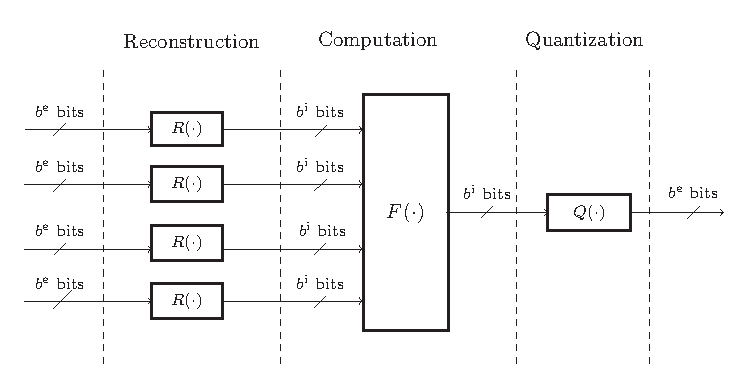
\includegraphics[width=30pc]{figures/Generalized_RCQ_Structure.eps}
    \caption{Illustration of a generalized RCQ unit which consists of three modules: \emph{Reconstruction} that maps a $b^{\text{e}}$-bit value to a $b^{\text{i}}$-bit value, \emph{Computation} that performs arithmetic operations, and \emph{Quantization} that quantizes a $b^{\text{i}}$-bit value to a $b^{\text{e}}$-bit value.}
    \label{fig: RCQ}
\end{figure}

\subsection{Generalized RCQ Unit}\label{sec: g-rcq}


 A generalized RCQ unit as  shown in Fig. \ref{fig: RCQ} consists of the following three modules:

\subsubsection{Reconstruction Module}\label{sec: recons}The reconstruction module applies a reconstruction function $R(\cdot)$ to each incoming $b^{\text{e}}$-bit external message to produce a $b^{\text{i}}$-bit internal message, where $b^\text{i}>b^\text{e}$. We denote the bit width of CN and VN internal message by $b^{\text{i,c}}$ and $b^{\text{i,v}}$, respectively. For the flooding-scheduled RCQ decoder, $R(\cdot)$ is iteration-specific and we use $R^{(t)}_\text{c}(\cdot)$ and $R^{(t)}_\text{v}(\cdot)$ to represent the reconstruction of check and variable node messages at iteration $t$, respectively. In the layer-specific RCQ decoder, $R(\cdot)$ uses distinct parameters for each layer in each iteration.  We use $R_\text{c}^{(t,r)}(\cdot)$ and $R_\text{v}^{(t,r)}(\cdot)$ to represent the the reconstruction of check and variable node messages at  layer $r$ of iteration $t$, respectively. The reconstruction functions are mappings of the input external messages to log-likelihood ratios (LLR) that will be used by the node.  In this paper, these mappings are systematically designed by HDQ discrete density evolution, which will be introduced in a later section.

For a quantizer $Q(\cdot)$ that is symmetric, an external message $d\in\mathbb{F}_2^{b^\text{e}}$ can be represented as $[d^{\text{MSB}}\ \tilde{d}]$, where $d^{\text{MSB}}\in\{0,1\}$ indicates sign and $\Tilde{d}\in\mathbb{F}_2^{b^\text{e}-1}$ corresponds to magnitude. We define the magnitude reconstruction function $R^*(\cdot):\mathbb{F}_2^{b^\text{e}-1}\rightarrow\mathbb{F}_2^{b^\text{i}-1}$, which maps the magnitude of external message, $\tilde{d}$, to the magnitude of internal message. Without loss of generality,  we restrict our attention to monotonic reconstruction functions so that
\begin{align}
    R^*(\tilde{d}_1)>R^*(\tilde{d}_2)>0,\quad \text{for }\tilde{d}_1>\tilde{d}_2,\label{r_mono}
\end{align}
where $\tilde{d}_1$, $\tilde{d}_2\in \mathbb{F}_2^{b^\text{e}-1}$. The reconstruction $R(d)$ can be expressed by
$R(d)=\left[d^{\text{MSB}}\ \ R^*(\tilde{d})\right]$.
Under the assumption of a symmetric channel, we have $R([0\ \Tilde{d}])=-R([1\ \Tilde{d}])$.
\subsubsection{Computation Module}
The computation module \texorpdfstring{$F(\cdot)$}{Lg} uses the $b^\text{\text{i}}$-bit outputs of the reconstruction module to compute a $b^\text{i}$-bit internal message for the CN or VN output. We denote the computation module implemented in CNs and VNs by $F_\text{c}$ and $F_\text{v}$, respectively. An RCQ decoder implementing the min operation at the CN yields a \minsum (ms) RCQ decoder. If an RCQ decoder implements belief propagation (bp) via the \textit{boxplus} operation, the decoder is called \textit{bpRCQ}. The computation module, $F_\mathrm{v}$, in the VNs is addition for both bpRCQ and msRCQ decoders.

If the RCQ decoder implements the \textit{Min} operation at the check node yielding a MinSum (ms) decoder, i.e.:
\begin{align}\label{equ: min}
    F_c(h_1,\ldots,h_J)=\prod_j\text{sign}(h_j)\times \min_{j}|h_j|,
\end{align}
where $h_j\in\mathbb{F}_2^{b^{i}}$, $j=1,...,J$ are internal messages, then we call the decoder an \emph{msRCQ} decoder.

If an RCQ decoder implements belief propagation (bp) via the \textit{boxplus} operation :
\begin{align}
    F_c(h_1,\ldots,h_J)=h_1 \boxplus h_2 \boxplus ... \boxplus h_J \label{equ: bp},
\end{align}
the decoder is called \textit{bpRCQ}. The operator $\boxplus$ is defined as:
\begin{align}
    h_1 \boxplus h_2 &= \log \left(\frac{1+e^{h_1+h_2}}{e^{h_1}+e^{h_2}}\right).
\end{align}
At variable node unit, both msRCQ and bpRCQ decoder sum up all incoming messages:
\begin{align}
    F_v(r_1,\ldots,r_J)=\sum_{j=1}^J r_j.
\end{align}
\subsubsection{Quantization Module} The quantization module \texorpdfstring{$Q(\cdot)$}{Lg} quantizes the $b^{\text{i}}$-bit internal message to produce a $b^{\text{e}}$-bit external message.
Under the assumption of a symmetric channel, we use a symmetric quantizer that features sign information and a magnitude quantizer $Q^*(\cdot)$.
The magnitude quantizer selects one of $2^{b^\text{e}-1}-1$ possible indexes using the threshold values $\{\tau_0,\tau_1,...,\tau_{\text{max}}\}$, where  $\tau_j\in\mathbb{F}_2^{b^{\mathrm{i}}}$ for $j\in\{0,1,...,2^{b^\text{e}-1}-2\}$ and $\tau_{\text{max}}$ is $\tau_{j_{\text{max}}}$ for $j_{\text{max}} = 2^{b^\text{e}-1}-2$.  We also require
\begin{align}
    {\tau}_i>{\tau}_j>0,\quad i>j.
\end{align}
Given an internal message $h\in\mathbb{F}_2^{b^{\mathrm{i}}}$, which can be decomposed into sign part $h^{\text{MSB}}$ and magnitude part $\tilde{h}$, $Q^*(\tilde{h})\in \mathbb{F}_2^{b^{\mathrm{e}}-1}$ is defined by:
\begin{align}
   {{Q^*(\tilde{h})}}=\left\{\begin{matrix}
 0,& \tilde{{h}} \leq {\tau}_0 \\ 
 j, &  {\tau}_{j-1} <  \tilde{{h}} \leq {\tau}_{j} \\
 2^{b^{\text{e}}-1}-1, & \tilde{h} >  {\tau}_{\text{max}}
\end{matrix}\quad,\right.\label{equ: quantization_mag}
\end{align}
where $0<j\le j_{\text{max}}$. Therefore, $Q(h)$ is defined by
$Q(h)=[h^{\text{MSB}}\ Q^*(\tilde{h})]$.
The super/subscripts introduced for $R(\cdot)$ also apply to $Q(\cdot)$. 
\subsection{Bit Width of RCQ decoder}
 The three tuple $(b^\text{e},b^{\text{i,c}}, b^{\text{i,v}})$ represents the precision of messages in a RCQ decoder. 
For the \emph{msRCQ} decoder, it is sufficient to use only the pair $(b^\text{e},b^{\text{i,v}})$ because $b^{\text{i,c}}=b^\text{e}$, we simply denote $b^{\text{i,v}}$ by $b^{\text{v}}$.   The CN min operation computes the XOR of the sign bits and finds the minimum of the extrinsic magnitudes. For a symmetric channel, the min operation can be computed by manipulating the external messages, because the external message delivers the  \emph{relative LLR meaning}  of reconstructed values.  Since we only use external messages to perform the min operation, $R^\text{c}(\cdot)$ and $Q^\text{c}(\cdot)$ are not needed for the {msRCQ decoder}. Finally, we use $\infty$ to denote a floating point representation. 

\subsection{FPGA Implementation for RCQ}
The RCQ FPGA decoder may be viewed as a modification to existing hardware decoders based on the BP or MS decoder algorithms, which have been studied extensively\cite{Zhang_undated-es,Sadek2016-lz,Liu2017-ho,Anantharaman2019-db}. 
The RCQ decoders require extra  $Q(\cdot)$ and $R(\cdot)$ functions to quantize and reconstruct message magnitudes. 
To implement  $Q(\cdot)$ and $R(\cdot)$ functions, we have devised the \emph{Lookup}, \emph{Broadcast}, and \emph{Dribble} methods. 
These three approaches are functionally identical, but differ in the way that the parameters needed for the $Q(\cdot)$ and $R(\cdot)$ operations are communicated to the nodes. 
\begin{figure}[h]
    \centering
      \subfloat[\label{recons_FPGA}]{%
        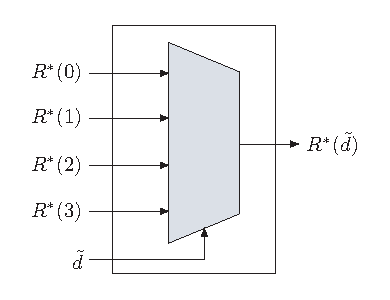
\includegraphics[width=.3\linewidth]{figures/Recons_logic.eps}}
  \subfloat[\label{quan_FPGA}]{%
       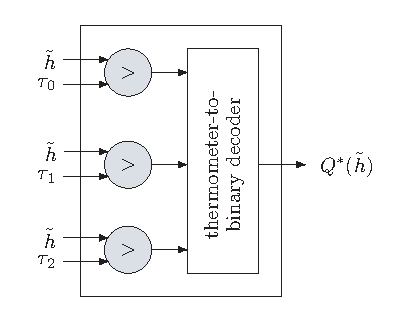
\includegraphics[width=.3\linewidth]{figures/Quantization_Logic.eps}}
  \\
  \subfloat[\label{t2b_FPGA}]{%
       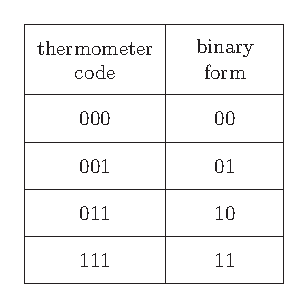
\includegraphics[width=.3\linewidth]{figures/thermometer-to-binary.eps}}
  \caption{msRCQ magnitude reconstruction module (a) and magnitude quantization module (b). In FPGA, magnitude reconstruction module is realized by a multiplexer, and  magnitude quantization is realized by comparison functions and  a thermometer-to-binary decoder which realizes the mapping relationship shown in (c).}
  \label{fig: FPGA}
\end{figure}
\subsubsection{Lookup Method}
The quantization and reconstruction functions simply map an input message to an output message.  Thus, a simple implementation uses lookup tables implemented using read-only memories (ROMs) to implement all these mappings.
As an example, for the iteration-specific magnitude quantizer $Q^{*(t)}(\cdot)$, all iterations can be implemented by a single table indexed by the pair $(\tilde{x},t)$, where $\tilde{x}$ is the internal message magnitude and $t$ is the current iteration. This index forms an address into a ROM to produce an output $\tilde{y}$.
The $Q(\cdot)$ and $R(\cdot)$ functions in every VN require their own ROMs, implemented using block RAMs. 
If block RAMs with multiple ports are available, then they can be shared by different VN banks to reduce the total amount required. If no ROM sharing occurs, then $L$ VN unit with two ROMs each results in a total of $2L$ additional block RAMs used. 
This amount can be reduced with ROM sharing and other synthesis techniques.
Because $Q(\cdot)$ and $R(\cdot)$ change with respect to different iterations and/or layers, one potential drawback of the Lookup method is a large block RAM requirement.  

\subsubsection{Broadcast Method}
The Broadcast method provides a scheme where all RCQ parameters are stored centrally in a control unit, instead of being stored in each VN.  
As an example, for the layered RCQ decoder whose parameters update every layer and iteration, the pair $(t,m)$, which corresponds to the current iteration and current layer, is used to index into ROMs in the control unit
These ROMs output quantization thresholds $\{\tau^{(t,m)}_0, \tau^{(t,m)}_1, \dots , \tau^{(t,m)}_{\text{max}}\}$ and reconstruction values $\{R^{(i,l)}(0), R^{(t,m)}(1), \dots , R^{(t,m)}(2^{b^c-1}-1)\}$, which are wired to the VN units. 
The $Q(\cdot)$ and $R(\cdot)$ blocks in the VN units only take in the parameters for each decoding iteration and layer, and use logic to perform their respective operations. 
Each VN only takes in the $Q(\cdot)$ and $R(\cdot)$ parameters necessary for decoding the current iteration and layer, and use logic to perform their respective operations. Fig. \ref{fig: FPGA} shows an implementation for a 3-bit RCQ, which uses mere 2 bits for magnitude reconstruction and quantization.
The $2$-bit magnitude reconstruction module  is realized by a $4\times1$ multiplexer. The $2$-bit magnitude quantization consists of two steps, first a  thermometer code\cite{Ajanya2018-uy}, where the contiguous ones are analogous to mercury in a thermometer, is generated by comparing the input with all thresholds, and then the thermometer code is converted to the  $2$-bit binary form by using a thermometer-to-binary decoder, which realizes the mapping relationship in Fig. \ref{t2b_FPGA}. 
Two block RAMS are required in the control unit for the thresholds and reconstruction values. Small LUTs in each VN implement the $Q(\cdot)$ and $R(\cdot)$ functions. The main penalty of the Broadcast method is the additional wiring necessary to route the RCQ parameters from the central control unit to the VNs.

The main penalty of the Broadcast is the additional wiring necessary to route the L-msRCQ parameters from the control unit to VN banks. If $w$ bits are used for each of the thresholds and reconstruction values of 3-bit L-msRCQ, a total of $7w$ additional wires need to be routed to each VN unit, $w$ wires for each of the three thresholds and each of the four reconstruction values.  With $L$ VN units, the total amount of added routes is $7wL$. For a 4-bit L-msRCQ decoder, the total increase is $15wL$. The same parameters are routed to all the VN units.  Thus shared wiring may be used in some cases.

\subsubsection{Dribble Method}
The Dribble method attempts to reduce the number of long wires required by the Broadcast method. Registers in the VNs save the current thresholds and reconstruction values necessary for the $Q(\cdot)$ and $R(\cdot)$ functions. Once again, quantization and reconstruction can be implemented using the logic in Fig. \ref{fig: FPGA}. When a new set of parameters is required, the bits are transferred (dribbled) one by one or in small batches from the control unit to the VN unit registers. Just as in the Broadcast method, two extra block RAMs and logic for the $Q(\cdot)$ and $R(\cdot)$ functions are required. 
But where the Broadcast method needs $7w$ additional wires routed to each VN bank for 3-bit L-msRCQ, the Dribble method requires only as many wires as the transfer batch size. 
The penalty of the Dribble method comes with the extra usage of registers in the VN units.
A total of $7w$ bits stored in registers would be necessary in each VN bank to save the current threshold and reconstruction values for 3-bit L-msRCQ. In total, $7wL$ bits of register storage would be used for 3-bit L-msRCQ, and $15wL$ bits would be necessary for 4-bit L-msRCQ. This total can be reduced by having multiple VN units share sets of registers.
We have implemented all methods and explored their  resource utilization in \cite{Terrill2021-ec}.


\section{Hierarchical Dynamic Quantization (HDQ) }\label{Sec: HDQ}
This section introduces the HDQ algorithm, a non-uniform quantization scheme that this paper uses both for quantization of channel observations and for quantization of internal messages by RCQ. Our results show, for example, that HDQ quantization of AWGN channel observations achieves performance similar to the optimal dynamic programming quantizer of \cite{Kurkoski2014-QuanDMC} for the binary input AWGN channel, with much lower computational complexity. 

\subsection{Motivation}
The quantizer plays an important role in RCQ decoder design. First, the channel observation is quantized as the input to the decoder. This section explores how to use HDQ to quantize the channel observations.  Second, the parameters of $R(\cdot)$ and $Q(\cdot)$ are also designed by quantizing external messages according to their probability mass function (PMF) as determined by discrete density evolution.  The use of HDQ to quantize internal messages is described in Section \ref{sec: layered}. 

The HDQ approach designs a quantizer that maximizes mutual information in a greedy or progressive fashion.  Quantizers aiming to maximize mutual information are widely used in non-uniform quantization design\cite{He2019-MIMQBP,Wang2020-RCQ,Lewandowsky2018-IBRegular,Stark2018-IBMA,Stark2020-IB5G,Meidlinger2015-MIMIB,Meidlinger2020-MINIBIRR,Meidlinger2017-MINIBIRR,Stark2020-IBjournal,Ghanaatian2018-MINIB-588, nathan-hdq, jiadong_softinfo_conf, jiadong_softinfo_jour}.
Due to the interest of this paper, the cardinality of quantizer output is restricted to $2^b$, i.e., this paper seeks $b$-bit quantizers.
Kurkoski and Yagi \cite{Tal2011-QuanVardy} proposed a dynamic programming method to find an {optimal} quantizer that maximizes mutual information for a binary input discrete memoryless channel (BI-DMC) whose outputs are from an alphabet with cardinality $B$,  with complexity $\mathcal{O}(B^3)$.
%while representing channel outputs from an alphabet with cardinality $B$ using an alphabet of $2^b$ quantized outputs 
The dynamic programming method of \cite{Kurkoski2014-QuanDMC} finds the optimal quantization, but the approach becomes impractical when $B$ is large. 



In order to quantize the outputs for a channel with large cardinality $B$ when constructing polar codes,  Tal and Vardy devised a sub-optimal greedy quantization algorithm with complexity  $\mathcal{O}(B\log(B))$ \cite{Tal2011-QuanVardy}. In \cite{Lewandowsky2018-IBRegular}, Lewandowsky \textit{et al.} proposed the modified Sequential Information Bottleneck (mSIB) algorithm to design the channel quantizer and LUTs for LDPC decoders. mSIB is also a sub-optimal quantization technique with complexity $\mathcal{O}(aB)$, where $a$ is the number of trials. As a machine learning algorithm, multiple trials are required for good results with mSIB.  Typical values of $a$ range, for example, from 15 to 70.

HDQ is proposed in \cite{Wang2020-RCQ} as an efficient $b$-bit quantization algorithm for the symmetric BI-DMC with complexity $\mathcal{O}\left(\frac{2^b}{\log(\gamma)}\log(B)\right)$. HDQ has less complexity than mSIB and also the Tal-Vardy algorithm. This section reviews the HDQ using symmetric binary input AWGN channel as an example. As an improvement to the HDQ of \cite{Wang2020-RCQ}, sequential threshold search is replaced with golden section search\cite{Kiefer1953-pc}.


\subsection{The HDQ Algorithm}
Let the encoded bit $x\in\{0,1\}$ be modulated by Binary Phase Shift Keying (BPSK) and transmitted over an AWGN channel. The modulated BPSK signal is represented as $s(x)=-2x+1$. We denote the channel observation at the receiver by $y$ where
\begin{align}
    y = s(x) +z,
\end{align}
and $z\sim \mathcal{N}(0,\sigma^2)$. The joint probability density function of $x$ and $y$, $f(x,y;\sigma)$, is:
\begin{align}
    f(x,y;\sigma) = \frac{1}{2\sqrt{2\pi \sigma^2}}e^{-\frac{(y-s(x))^2}{2\sigma^2}}.
\end{align}


HDQ seeks an $b$-bit quantization of the continuous channel output $y$, as in \cite{jiadong_softinfo_conf}.  In practice, often $y$ is first quantized into $B$ values using high-precision uniform quantization where $B\gg 2^b$, i.e., analog-to-digital (A/D) conversion.   Let $W$ be the result of the A/D output, where $W\in \mathcal W $ and  ${\mathcal W} =\{0,1,...,B-1\}$. 
The alphabet of $B$ channel outputs from the A/D converter is then subjected to further non-uniform quantization resulting in a quantization alphabet of $2^b$ values. We use $D$ to represent the non-uniform quantizer output, which is comprised of the $b$ bits $ D=[D_1,...,D_b]$.  HDQ aims to maximize the mutual information between $X$ and $D$.
% \begin{align}
%     \arg\max_{Q\in\mathcal{Q}} I(X;D).
% \end{align}

For the symmetric binary input AWGN channel, a larger index $w$ implies a larger LLR, i.e.:
\begin{align}\label{equ: inq}
    \log \frac{P_{W|X}(i|0)}{P_{W|X}(i|1)}<\log \frac{P_{W|X}(j|0)}{P_{W|X}(j|1)},~ \forall i<j.
\end{align}
Based on Lemma 3 in \cite{Kurkoski2014-QuanDMC}, any binary-input discrete memoryless channel that satisfies \eqref{equ: inq} has an optimal $b$-bit quantizer that is determined by $2^b-1$ boundaries, which can be identified by their corresponding index values.  Denote the $2^{b}-1$ index thresholds by $\{\xi_{1}$, $\xi_{2},..., \xi_{2^{b}-1} \} \subset {\mathcal W}$. Unlike the dynamic programming algorithm\cite{Kurkoski2014-QuanDMC}, which optimizes boundaries jointly, HDQ \textit{sequentially} finds thresholds according to \textit{bit level}, similar to the progressive quantization in \cite{nathan-hdq}.



\begin{figure}
	\centering
	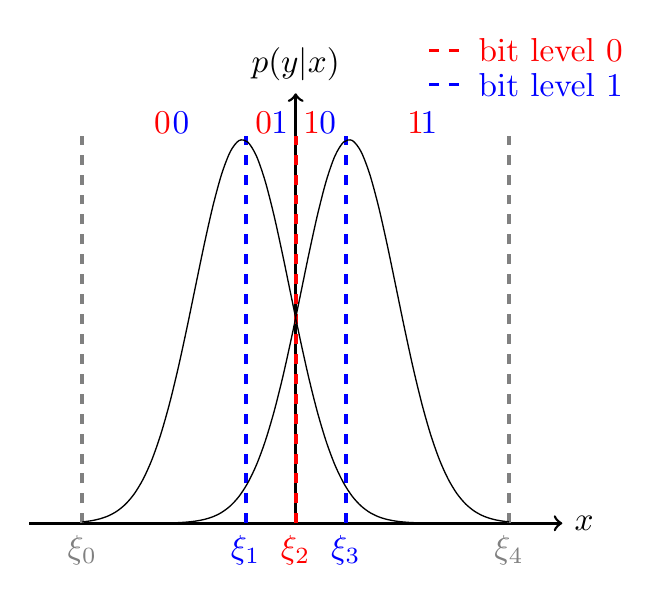
\begin{tikzpicture}[scale = 1.2]
    \begin{axis}[every axis plot post/.append style={
      mark=none,domain=-4:4,samples=50,smooth},
    clip=false,
    axis y line=none,
    axis x line*=bottom,
    ymin=0,
    xtick=\empty,
    ]
    %\draw[help lines, color=gray!30, dashed] (-4.9,0) grid (4.9,0.5);
    \draw[->, thick] (-5,0)--(5,0) node[right]{$x$};
    \draw[->, thick] (0,0)--(0,0.5) node[above]{$p(y|x)$};
    \draw[very thick, dashed, color = red] (0,0)--(0,0.45);
    \node [below, color = red] at (0,0) {{$\xi_2$}};
    \draw[very thick, dashed, color = blue] (0.9400,0)--(0.9400,0.45);
    \node [below, color = blue] at (0.9400,0) {{$\xi_3$}};
    \draw[very thick, dashed, color = blue] (-0.9400,0)--(-0.9400,0.45);
    \node [below, color = blue] at (-0.9400,0) {{$\xi_1$}};
    \draw[very thick, dashed, color = gray] (4,0)--(4,0.45);
    \node [below, color = gray] at (4,0) {{$\xi_4$}};
    \draw[very thick, dashed, color = gray] (-4,0)--(-4,0.45);
    \node [below, color = gray] at (-4,0) {{$\xi_0$}};
    \addplot [color=black] {\gauss{1}{0.8944}};
    \addplot [color=black] {\gauss{-1}{0.8944}};
    \draw[ thick, dashed, color = red ] (2.5,0.55)--(3.2,0.55) node[right]{bit level 0};
    \draw[ thick, dashed, color = blue ] (2.5,0.51)--(3.2,0.51) node[right]{bit level 1};
    \node [above, color = red] at (-2.5,0.44) {0};
    \node [above, color = blue] at (-2.15,0.44) {0};
    \node [above, color = red] at (-0.6,0.44) {0};
    \node [above, color = blue] at (-0.30,0.44) {1};
    
    
    \node [above, color = blue] at (2.5,0.44) {1};
    \node [above, color = red] at (2.25,0.44) {1};
    \node [above, color = blue] at (0.6,0.44) {0};
    \node [above, color = red] at (0.30,0.44) {1};
    
    \end{axis}
    \end{tikzpicture}
	\caption{Given the conditional probability $p(y|x)$ of symmetric BI-AWGN channel, HDQ sequentially quantizing A/D output $w$ into a 2-bit message by first finding the index $\xi_2$, then the indices $\xi_1$ and $\xi_3$.}
	\label{fig: HDQ}
\end{figure}

HDQ quantizes the symmetric BI-AWGN channel output using a  progressive \cite{nathan-hdq} or greedy approach.  
The general $b$-bit HDQ approach is as follows:
\begin{enumerate}
    \item We assume an initial high-precision uniform quantizer.  For this case, set the extreme index thresholds  $\xi_0=0$ and $\xi_{2^b}=B-1$, which are the minimum and maximum outputs of the uniform quantization.  
    \item The index threshold $\xi_{2^{(b-1)}}$ is selected as follows to determine the bit level 0:
    \begin {align}
    \xi_{2^{(b-1)}} = \arg \max_{\xi_0<\xi<\xi_{2^b}} I(X;D_1)\, , 
    \end{align}
where 
\begin{equation} 
D_1 = \mathbbm{1}(W\geq \xi_2^{(b-1)}).
% D_1 = \begin{cases} 
% 0, & \text{if } W < \xi_{2^{(b-1)}}\\
% 1, & \text{otherwise}
%\end{cases}.
\end{equation}

\item The index thresholds  $\xi_{2^{(b-2)}}$ and $\xi_{3*2^{(b-2)}}$ are selected as follows to determine bit level 1:
    \begin {align}
    \xi_{2^{(b-2)}} &= \arg \max_{\xi_0<\xi<\xi_{2^{b-1}}} I(X;D_2| D_1=0), \\ 
    \xi_{3*2^{(b-2)}} &= \arg \max_{\xi_{2^{b-1}}<\xi<\xi_{2^b}} I(X;D_2| D_1=1)\, ,
    \end{align}
    and 
\begin{equation} 
D_2 = \begin{cases} 
\mathbbm{1}(W \geq \xi_{2^{(b-2)}}) & \text{if } D_1=0 \\
\mathbbm{1}(W \geq \xi_{3*2^{(b-2)}}) & \text{if } D_1=1 \\
\end{cases}.
\end{equation}

\item In the general case, when the thresholds for $k$ previous quantization bits have been determined, $2^k$ thresholds $\{\xi_{(j+0.5)2^{b-k}}, j=0,..,2^{k}-1\}$ must be selected to determine the next quantization bit.  Each threshold maximizes $I(X;D_{k+1}|D_k=d_k, \ldots,D_1=d_1 )$ for a specific result for the $k$ previous quantization bits. 
\end{enumerate}


\begin{algorithm}[t]
    \label{alg: HDQ}
    \SetKwInOut{Input}{input}\SetKwInOut{Output}{output}\SetKwProg{Init}{initialization:}{}{}
    
    \Input{$P\left(X,W\right), X\in\{0,1\}, W\in\{0,...,B-1\}$; $b$}
    \Output{ $\{\xi_0,\xi_1,...,\xi_{2^b-1}\}$, $P(X,T)$}
    $\xi_0\leftarrow 0$, 
    $\xi_{2^b}\leftarrow B-1$\\
    \For{$i\gets0$ \KwTo $b-1$ }{
        \For{$j\gets0$ \KwTo $2^{i}-1$ }{
        $\xi_{(j+0.5)2^{b-i}} = \texttt{GSS}(\xi_{j2^{b-i}},\xi_{(j+1)2^{b-i}})$
        }
        }
    $P_{XT}(x,t)=\sum_{w=\xi_t}^{\xi_t+1}P_{XW}(x,w)$, $X\in\{0,1\}$, $T\in\{0,...,2^{b-1}\}$
    \caption{Hierarchical Dynamic Quantization }
    \end{algorithm}
Fig. \ref{fig: HDQ} illustrates how HDQ quantizes the symmetric binary input AWGN for the case where $b=2$. First, the indices  $\xi_0$  and $\xi_4$ of the extreme points are set.  Then the index $\xi_2$ is set to maximize $I(X;D_1)$.  Finally, the indices $\xi_1$ and $\xi_3$ are set to maximize $I(X;D_2| D_1)$ by independently selecting $\xi_1$ to maximize $I(X;D_2| D_1=0)$ and $\xi_3$ to maximize $I(X;D_2| D_1=1)$.


Alg. \ref{alg: HDQ} provides a full description of HDQ algorithm. The function \texttt{GSS}$(\xi_{\ell},\xi_r)$ uses the golden section search algorithm described in Sec.\ref{Sec: GSS} for thresholds search.

HDQ provides the $2^b -1$ index thresholds $\{\xi_1, \ldots, \xi_{2^b-1} \}$. For channel quantization, the index thresholds can be mapped to channel outputs. For the RCQ decoding, the messages are LLR values, the LLR magnitude thresholds $\{\tau_0,\ldots,\tau_{2^{b-1}-2}\}$ are calculated from the index thresholds $\{\xi_{2^{b-1}+1}, \ldots ,\xi_{2^b-1} \}$ as follows:
\begin{align}
\tau_i =~ \log\frac{P_{W|X}(\xi_{1+i+2^{b-1}}|0)}{P_{W|X}(\xi_{1+i+2^{b-1}}|1)}, i=0,1,\ldots,2^{b-1}-2.
\end{align}

HDQ also provides the joint probability between code bit $X$ and quantized message $D$, $P(X,D)$. The magnitude reconstruction function  $R^*(\cdot)$ is computed as follows: 
%to produce LLR magnitudes from quantized messages 
\begin{align}
    R^*(d) = \log\frac{P_{XT}(0,d+2^{b-1})}{P_{XT}(1,d+2^{b-1})},~d=0,1,...,2^{b-1}-1.
    \label{equ: recon_hdq}
\end{align}


\begin{figure}[t]
	\centering
	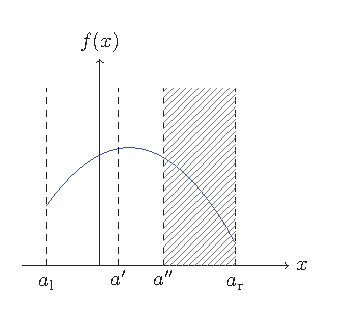
\includegraphics[width=0.5\linewidth]{figures/gss.eps}
	\caption{ Illustration of one iteration of golden-section search for finding maximum point of $f(x)$ in the interval $[a_\text{l},a_\text{r}]$. $a'=a_{\text{r}}-\frac{a_\text{r}-a_\text{l}}{\gamma}$ and $a''=a_{\text{l}}+\frac{a_\text{r}-a_\text{l}}{\gamma}$. Because $f(a'')<f(a')$, $[a'',a_\text{r}]$ is truncated and $[a_\text{l},a'']$ becomes the new search interval for the next iteration. 
	}
	\label{fig: gss}
\end{figure}

\subsection{Golden-Section Search and Complexity Analysis}\label{Sec: GSS}
After $k$ stages of HDQ, there are $2^k$ quantization regions each specified by their leftmost and rightmost indices $\xi_{\ell}$ and $\xi_r$.  The next stage finds a new threshold $\xi^*$ for each of these $2^k$ regions.   Each $\xi^*$ is selected to maximize a conditional mutual information as follows:
    \begin{equation}
    \xi^* = \arg \max_{\xi_{\ell}<\xi<\xi_r}  I(\xi),
    \label{equ: optimzation}
    \end{equation}
where 
\begin{align}
      I(\xi) &= I\left(X;D_{k+1}(\xi)|D_1=d_1, \ldots,D_k=d_k \right)\label{equ: I_xi} \\
    &= \sum_{x,d_{k+1}} P\left(x,d_{k+1}(\xi)|d_1^k\right) \log  \frac{P(d_{k+1}(\xi)|x,d_1^k) }{P(d_{k+1}(\xi)|d_1^k) }
\end{align}
for the binary $k$-tuple $d_1^k=d_1, \ldots, d_k$  that defines $(\xi_{\ell}, \xi_r)$. The probability $P\left(x,d_{k+1}(\xi)|d_1^k\right)$ is defined as follows:

\begin{equation}
    P\left(x,d_{k+1}(\xi)|d_1^k\right) = 
    \begin{cases}
    \frac{\sum_{w=\xi_l}^{\xi} P_{XW}(x,w)}{\sum_{w=\xi_l}^{\xi_r} P_{W}(w)} & d_{k+1}=0\\
    \frac{\sum_{w=\xi+1}^{\xi_r} P_{XW}(x,w)}{\sum_{w=\xi_l}^{\xi_r} P_{W}(w)} & d_{k+1}=1\\
    \end{cases}.
\end{equation}

Because $I(\xi)$ is concave in $\xi$, the local maximum can be found using the golden section search \cite{Kiefer1953-pc}, a simple but robust technique to find extreme point of a unimodal function by successively narrowing the range of values on a specified interval. Specifically, Fig. \ref{fig: gss} illustrates one iteration of golden-section search for finding maximum point of $f(x)$ in the interval $[a_\text{l},a_{\text{r}}]$. First, find $a'=a_{\text{r}}-\frac{a_\text{r}-a_\text{l}}{\gamma}$ and $a''=a_{\text{l}}+\frac{a_\text{r}-a_\text{l}}{\gamma}$, where $\gamma = \frac{\sqrt{5}+1}{2}$. Because $f(a'')<f(a')$, which suggests that the maximum point lies in $[a_\text{l},a'']$, the interval $[a'',a_\text{r}]$ is truncated and  $[a_\text{l},a'']$ is updated as the next round search interval. Further details of golden-section search can be found in \cite{Kiefer1953-pc}. When using the golden-section search to find all $2^b -1$ thresholds for the $b$-bit HDQ, $I(\xi)$ will be computed using \eqref{equ: I_xi} a number of times that is proportional to: 
\begin{align}
    &\log_{\gamma}(B)+\sum_{i=1}^{2^1}\log_{\gamma}(B_{2,i})+\ldots+\sum_{i=1}^{2^{b-1}}\log_{\gamma}(B_{b,i}),\\
   =&\log_{\gamma}(B)+\log_{\gamma}\prod_{i=1}^{2^1}B_{2,i}+\ldots+\log_{\gamma}\prod_{i=1}^{2^{b-1}}B_{b,i},\\
    \leq&\log_{\gamma}(B)+2\log_{\gamma}\left(\frac{B}{2}\right)+\ldots+2^{b-1}\log_{\gamma}\left(\frac{B}{2^{b-1}}\right)\\=& \frac{2^b}{\log(\gamma)}\log(B).
\end{align}

$B_{j,i}$ is the $i^{th}$ interval length in ${j-1}$ bit level quantization and $\sum_{i=1}^{2^{j-1}}B_{j,i}=B$. Therefore, a $b$-bit quantization on a  $B$-output channel using HDQ can be designed in $\mathcal{O}\left(\frac{2^b}{\log(\gamma)}\log(B)\right)$ time.
\begin{figure}[t]
	\centering
	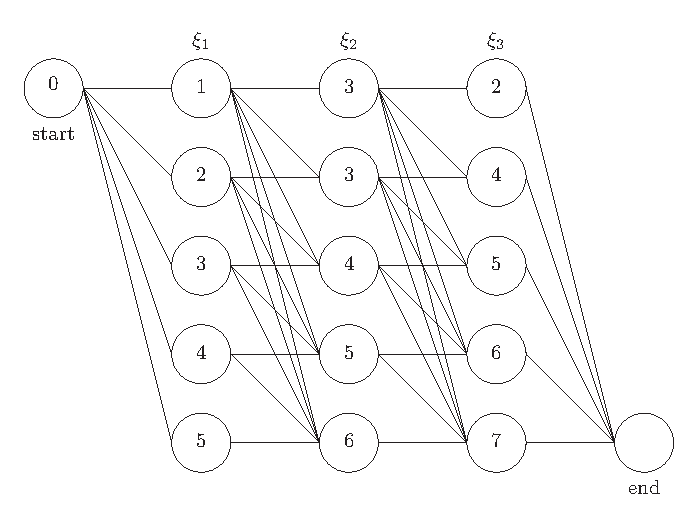
\includegraphics[width=0.5\linewidth]{figures/trellis.eps}
	\caption{A trellis whose paths represent all 2-bit quantizers for a BI-DMC with 8 outputs. The vertices in column $i$ are possible values for $i^{th}$ threshold $\xi_i$. Each branch in the trellis identifies a quantization region.
	}
	\label{fig: trellis}
\end{figure}

\subsection{Comparing HDQ with Optimal Dynamic Programming}
Unlike the dynamic programming approach of Kuskoski and Yagi \cite{Kurkoski2014-QuanDMC}, HDQ does not always provide the optimal solution.  
This subsection provides an example contrasting HDQ with the dynamic programming solution. 
Following \cite{Kurkoski2014-QuanDMC}, Fig. \ref{fig: trellis} gives a trellis whose paths represent all 2-bit quantizers for a binary input DMC with 8 outputs. The outputs are indexed from 0 to 7 and satisfy \eqref{equ: inq}. The vertices in column $i$ are possible values for $\xi_i$, and each path represents a valid quantizer whose thresholds are determined by the vertices in each column. Each branch in the trellis identifies a quantization region. For example, the branch connecting vertex $\xi_0=0$ to vertex $\xi_1=2$ specifies the leftmost quantization region as \{0,1\}, i.e., $\xi_{\ell} = 0$ and $\xi_r =1$.



%  Kurkoski's dynamic programming algorithm searches whole trellis and finds the optimal path that maximizes $I(X;D_1,D_2)$. 
The dynamic programming algorithm determines vertices of all columns jointly, whereas HDQ identifies the vertices in a greedy way, by first finding the vertex in column 2 to maximize $I(X;D_1)$ and then vertices in column 1 and 4 to maximize $I(X;D_2|D_1=d_1)$.  Hence, the greedy approach of HDQ only searches part of trellis and therefore is sub-optimal. However, our simulations show that HDQ finds the quantizer that perform closely to  the optimal one.


\begin{figure}[htp] 
    \centering
  \subfloat[\label{fig: quan_result}]{%
       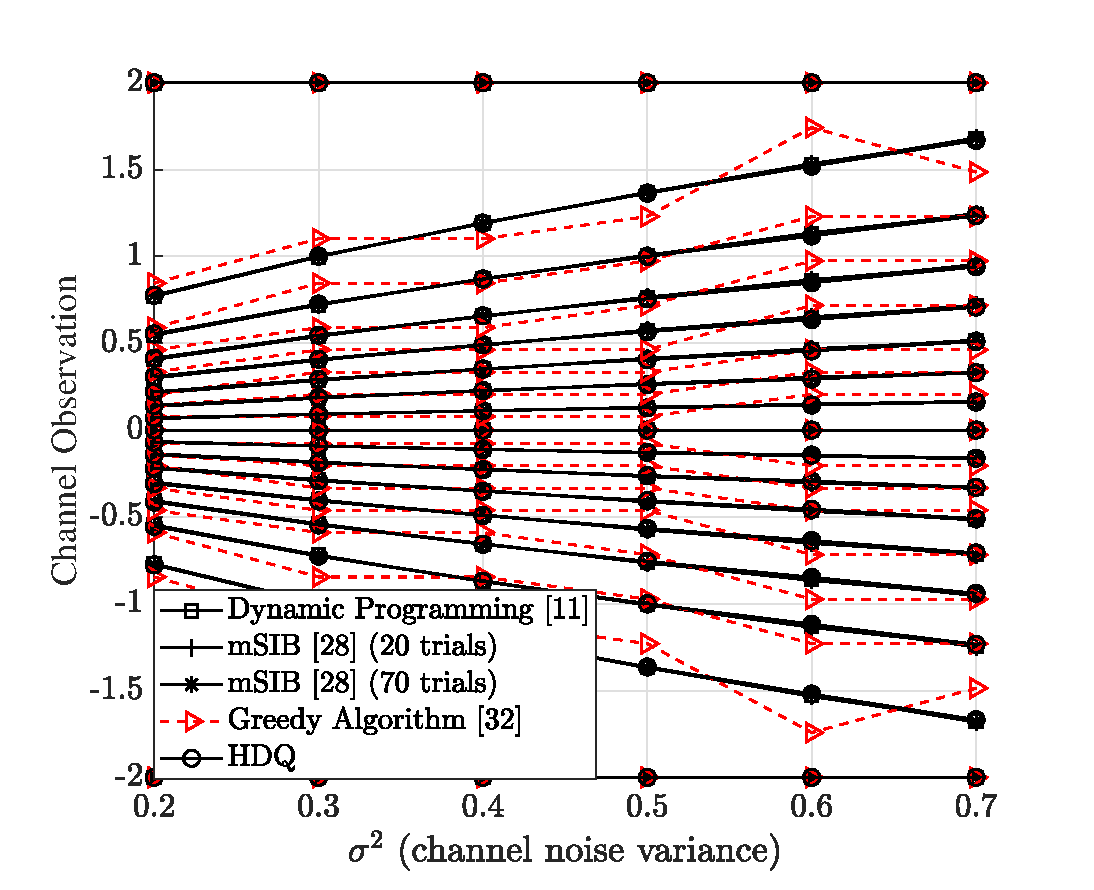
\includegraphics[width=0.5\linewidth]{figures/quantization_result.eps}}
   \\
  \subfloat[\label{fig: mi_loss}]{%
        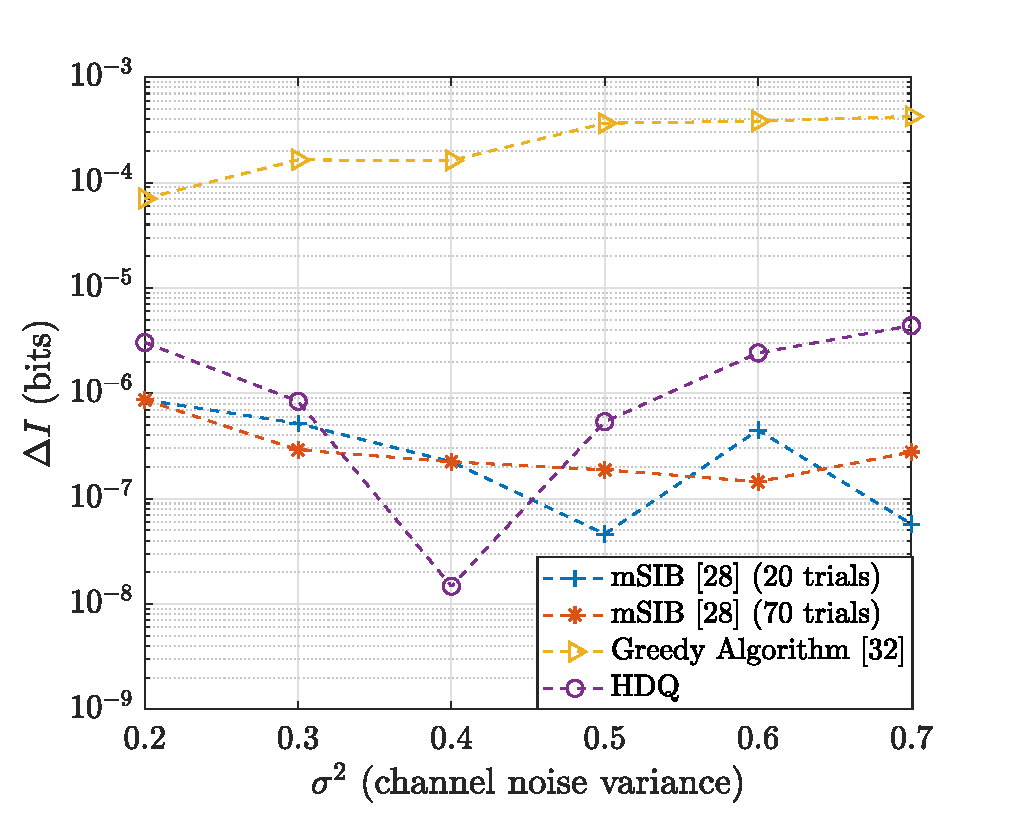
\includegraphics[width=0.5\linewidth]{figures/mutual_info_loss.eps}}
  \caption{Fig. (a): Quantization thresholds for dynamic programming, msIB, and HDQ on the BI-AWGNC as a function of $\sigma^2$ for $B=2000$. Fig. (b): Mutual information loss between each sub-optimal quantizer and optimal quantizer for BI-AWGNC as a function of $\sigma^2$ for $B=2000$. }
\end{figure}

\subsection{Simulation Result}
This section provides simulation results for quantizing symmetric binary input AWGN channel observations. The simulations compare HDQ to the optimal dynamic programming result as well as to two sub-optimal approaches: mSIB with 20 and 70 trials and the greedy quantization algorithm describe in \cite{Lewandowsky2018-IBRegular}. For all the quantization approaches, the channel observations are first quantized uniformly into $B=2000$ points between $-2$ and $2$. 

Fig. \ref{fig: quan_result} gives the thresholds as a function of $\sigma^2$ for HDQ, dynamic programming, mSIB with 20 and 70 trials, and  greedy quantization.  The quantization thresholds for HDQ, dynamic programming, and mSIB are indistinguishable in Fig.  \ref{fig: quan_result}.  HDQ has significantly lower complexity than both dynamic programming and mSIB. The thresholds for greedy quantization algorithm of \cite{Tal2011-QuanVardy} deviate noticeably from the thresholds found by the other approaches.


In order to quantify the performance of sub-optimal quantizers, we define $\Delta I$ as follows:
\begin{align}
    \Delta I = I^{\text{dp}}(X;D)-I^{\text{sub}}(X;D),
\end{align}
where $I^{\text{dp}}(X;D)$ and $I^{\text{sub}}(X;D)$ are the mutual information between code bit $X$ and quantized value $D$ as obtained by dynamic programming and sub-optimal quantizers, respectively. Fig. \ref{fig: mi_loss} plots $\Delta I$ as a function of $\sigma^2$ for each sub-optimal quantizer.  All three sub-optimal quantizers perform quite well with $\Delta I < 10^{-3}$ bits.  However, HDQ and mSIB achieve  $\Delta I < 10^{-6}$, significantly outperforming the greedy approach of \cite{Tal2011-QuanVardy}.

\section{Flooding-scheduled RCQ Decoder}\label{sec: MIM-DDE}
RCQ decoder is a result of quantized density evolution: In the $t^{th}$ iteration, the quantization functions and the reconstruction functions associated with that iteration, i.e., $Q^c_{t}$, $R^v_t$, $Q^v_t$, $R^v_{t+1}$ are constructed by quantizing the joint p.m.f. between code bits and the message from either the variable node or check node. These functions are also the parameters of the flooding-scheduled RCQ decoder.  To differentiate our discrete density evolution from the one using uniform quantization\cite{Sae-Young_Chung2001-DDE0045}, we name our density evolution \textit{HDQ Discrete Density Evolution} (HDQ-DDE).  Specifically, this section describes the HDQ-DDE when the check node uses box-plus operation. The decoder generated by such HDQ-DDE is a flooding-scheduled bpRCQ decoder.

\subsection{MIM-DDE at check node}
Denote the joint p.m.f between the \textit{external message} from the $i^{th}$ variable node and corresponding code bit  by $P^{v,i}(X,T)$, $X=\{0,1\}$, $T=\{0,\ldots,2^m-1\}$. Based on the independence assumption in density evolution \cite{Richardson2001-de}, all incoming messages have same distribution:
\begin{align}
    P^{v,i} (X,T)=P^v(X,T),\quad i=0,...,d_c-2
\end{align}
where $d_c$ is check node degree. At check node, the code bit corresponding to output is the XOR sum of code bits corresponding to all inputs. By denoting:
\begin{align}
    P^{v,a}(X,T)\circledast P^{v,b}(X,T)\triangleq\sum_{\substack{m,n:\\m\bigoplus n=k} }P^{v,a}(X_m,T)P^{v,b}(X_n,T),
\end{align}
where $m,n,k\in\{0,1\}$, the joint p.m.f between code bit corresponding to output and input messages, $P^c_{out}(X,\mathbf{T})$, can be represented by:
\begin{align}
    P^c_{out}(X,\mathbf{T})&=P^{v,0}(X,T)\circledast ...\circledast P^{v,d_c-2}(X,T)\\
    &=P^{v}(X,T)\circledast ...\circledast P^{v}(X,T)\\
    &\triangleq P^v(X,T)^{\circledast(d_c-1)}, \label{equ: check_opt_prob}
\end{align}
where $\mathbf{T}$ is a vector containing all incoming $d_c-1$ messages.

In order to keep the cardinality of external message the same, $P^c_{out}(X,\mathbf{T})$ needs to be quantized to $2^m$ levels. As pointed in \cite{Lewandowsky2018-IBRegular}, $|\mathbf{T}|=2^{m(d_c-1)}$ will be very large when $m$ and $d_c$ is large. For an example, if $d_c=8$ and $m=4$, $|\mathbf{T}|=2.68*10^8$. Hence, directly quantizing $P^c_{out}(X,\mathbf{T})$ is impossible. To mitigate the problem of \textit{cardinality bombing}, we propose an intermediate coarse quantization algorithm called One-Step-Annealing (OSA) quantization without sacrificing mutual information. Note that Eq. (\ref{equ: check_opt_prob}) can be calculated in a recursive way and each step takes two inputs:
\begin{align}
\label{equ: check_recur}
    P_{out}^{c}(X,\mathbf{T})^{\circledast i}=P^v(X,T)^{\circledast (i-1)}\circledast P^v(X,T) 
\end{align}
We observe that, in each step, the output of Eq.(\ref{equ: check_recur}) has some entries with very close log likelihood ratio (LLR) values. By merging entries whose LLR difference is small enough, mutual information loss is negligible.  Hence, OSA simply merges entries whose LLR values difference is less than a threshold $l_s$, and the output of OSA will be the input of the next p.m.f calculation step, i.e.:
\begin{align}
\label{equ: check_osa}
    P^{v}(X,T)^{\circledast i}= \texttt{OSA}(P^v(X,T)^{\circledast (i-1)},l_s)\circledast P^v(X,T).
\end{align}
\begin{algorithm}[t]
    \label{alg: OSA}
    \SetKwInOut{Input}{input}\SetKwInOut{Output}{output}\SetKwProg{Init}{initialization:}{}{}
    
    \Input{$\Pr\left(X,Y\right), X\in\{0,1\}, Y\in\{0,...,N-1\}$; $l_s$}
    \Output{$\Pr(X,T)$}
    $j\leftarrow0$, 
    $\Pr(X_0,T_j)\leftarrow P(X_0,Y_0)$,
    $\Pr(X_1,T_j)\leftarrow P(X_1,Y_0)$, 
    $l\leftarrow  \log\frac{\Pr(X_0,Y_0)}{\Pr(X_1,Y_0)}$
    
    \For{$i\gets1$ \KwTo $N-1$ }{
          \eIf{$(\log\frac{P(X_0,T_i)}{P(X_1,T_i)}-l)\leq l_s$}
        {
        $P(X_0,T_j)\leftarrow\Pr(X_0,T_j)+\Pr(X_0,Y_i)$, 
        $P(X_1,T_j)\leftarrow\Pr(X_1,T_j)+\Pr(X_1,Y_i)$
        }
        {
        $j\leftarrow j+1$\\
        $\Pr(X_0,T_j)\leftarrow\Pr(X_0,Y_i)$, $\Pr(X_1,T_j)\leftarrow\Pr(X_1,Y_i)$\\
        $l\leftarrow\log\frac{\Pr(X_0,Y_i)}{\Pr(X_1,Y_i)}$
        }
        }
    \caption{One Step Annealing Algorithm (OSA) }\label{sec: MIMDDE}
\end{algorithm}
\begin{figure}
	\centering
	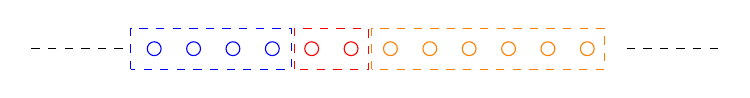
\begin{tikzpicture}[scale = 2.0]


\node[circle,draw=blue, fill=white, inner sep=0pt,minimum size=5pt] (b) at (-1,0) {};
\node[circle,draw=blue, fill=white, inner sep=0pt,minimum size=5pt] (b) at (-0.25,0) {};
\node[circle,draw=blue, fill=white, inner sep=0pt,minimum size=5pt] (b) at (-0.5,0) {};
\node[circle,draw=blue, fill=white, inner sep=0pt,minimum size=5pt] (b) at (-0.75,0) {};
\node[circle,draw=red, fill=white, inner sep=0pt,minimum size=5pt] (b) at (0,0) {};
\node[circle,draw=red, fill=white, inner sep=0pt,minimum size=5pt] (b) at (0.25,0) {};
\node[circle,draw=orange, fill=white, inner sep=0pt,minimum size=5pt] (b) at (0.5,0) {};
\node[circle,draw=orange, fill=white, inner sep=0pt,minimum size=5pt] (b) at (0.75,0) {};
\node[circle,draw=orange, fill=white, inner sep=0pt,minimum size=5pt] (b) at (1,0) {};
\node[circle,draw=orange, fill=white, inner sep=0pt,minimum size=5pt] (b) at (1.25,0) {};
\node[circle,draw=orange, fill=white, inner sep=0pt,minimum size=5pt] (b) at (1.5,0) {};
\node[circle,draw=orange, fill=white, inner sep=0pt,minimum size=5pt] (b) at (1.75,0) {};
\draw[black, dashed] (2.0,0)--(2.6,0);
\draw[black, dashed] (-1.2,0)--(-1.8,0);
\draw [blue, dashed] (-1.15,-0.13) rectangle (-0.13,0.13);
\draw [red, dashed] (-0.11,-0.13) rectangle (0.36,0.13);
\draw [orange, dashed] (0.38,-0.13) rectangle (1.86,0.13);
\end{tikzpicture}
	\caption{OSA illustration: points are ordered w.r.t. LLR values. Each color represents a cluster and LLR value difference in each cluster is less than $l_s$. }
	\label{fig: OSA}
\end{figure}

We use $l_s\in[10^{-4},10^{-3}]$ in our simulation. Fig. \ref{fig: OSA} shows an illustration of OSA and a full description of the OSA algorithm is given in Algorithm \ref{alg: OSA}. The following table shows $|\mathbf{T}|$ after we implement OSA and choose different $l_s$. The example we show has the parameter $m=4$, $d_c=8$. The result shows that OSA greatly decreases the output cardinality, and based on our simulation, mutual information losses under these three $l_s$ are all less than $10^{-7}$ bits.

\begin{table}[h!]
    \centering
    \begin{tabular}{|c|c|c|c|c|}
        \hline
        $l_s$                                                             & $0$           & $10^{-4}$  & $5*10^{-4}$ & $10^{-3}$  \\ \hline
        \begin{tabular}[c]{@{}c@{}}$|\mathbf{T}|$\end{tabular} & $2.68*10^{8}$ & $3.3*10^4$ & $1.7*10^3$  & $1.3*10^3$ \\ \hline
    \end{tabular}
\end{table}

\subsection{MIM-DDE at variable node}

Each variable node sums the LLR messages from its channel observation and neighboring check nodes. By denoting: 

\begin{align}
P^{c,a}(X,T)\boxdot P^{c,b}(X,T)&=\frac{1}{P(X)}P^{c,a}(X,T)P^{c,b}(X,T),
\end{align}
the joint p.m.f between code bit $X$ and incoming message combination $\mathbf{T}$, $P^v_{out}(X,\mathbf{T})$, given variable node degree $d_v$,  can be expressed by:
\begin{align}
    P^v_{out}(X,\mathbf{T})=P^{ch}(X,T)\boxdot P^c(X,T)^{\boxdot(d_v-1)},
\end{align}
Similarly, for irregular LDPC codes with variable edge degree distribution 
\begin{align}
    \lambda(x)=\sum_{i=2}^{d_{v,max}}\lambda_ix^{i-1},
\end{align}
$P^v_{out}(X,\mathbf{T})$ is given by:
\begin{align}
     P^v_{out}(X,\mathbf{T})=P^{ch}(X,T)\boxdot \sum_{i=2}^{d_{v,max}}\lambda_i P^c(X,T)^{\boxdot(d_v-1)}.
\end{align}
$P_{out}^v(X,\mathbf{T})$ is then quantized to $2^m$ levels by HDQ. Also, as a result of HDQ, and joint p.m.f between code bit $X$ and quantized messages $T$, $P^v(X,T)$, is updated. $Q^v$ in this iteration and $R^c$ in the next iteration are built correspondingly. Note that variable nodes also face the \textit{cardinality bombing} problem, hence $\texttt{OSA}$ is needed in each  recursive step. 



Thus, by implementing MIM-DDE, we can iteratively update $P^c(X,T)$, $P^v(X,T)$ and build $Q^c_i$, $Q^v_i$, $R^c_i$ and $R^v_i$, $i=\{0,...,I_T-1\}$. 

In MIM-DDE, we only limit the precision of external messages, i.e. $m$, and keep internal messages, $n^c$ (only for \textit{bp-RCQ}) and $n^v$, full precision. To make internal message precision finite, a uniform $n^c$ (or $n^v$) quantizer is required when implementing ${F}^c$(or ${F}^v$).

\subsection{Threshold}
At any specified $\frac{E_b}{N_o}$, flooding-scheduled HDQ discrete density evolution constructs the $R^{(t)}(\cdot)$ and $Q^{(t)}(\cdot)$ functions  at each iteration $t$ and also computes the mutual information $I^{(t)}\left(\frac{E_b}{N_o}\right)$ between a code bit and its corresponding variable node message in each layer $r$ at each iteration $t$. An important design question is which value of $\frac{E_b}{N_o}$ to use to construct the $R^{(t)}(\cdot)$ and $Q^{(t)}(\cdot)$ functions implemented at the decoder, which necessarily will work over a range of $\frac{E_b}{N_o}$ values in practice.  Define the threshold of a flooding RCQ decoder given a maximum number of decoding iterations $I_T$ as: 
\begin{align}
    \frac{E_b}{N_o}^*=\inf \left\{\frac{E_b}{N_o}:  I^{(I_T)}\left(\frac{E_b}{N_o}\right)> 1-\epsilon\right\},
\end{align}
i.e., $\frac{E_b}{N_o}^*$ is the smallest $\frac{E_b}{N_o}$ that achieves a mutual information between the  code bit and the external message that is greater that $1-\epsilon$. Our simulation results show that  $\frac{E_b}{N_o}^*$ for $\epsilon = 10^{-4}$ produced $R^{(t)}(\cdot)$ and $Q^{(t)}(\cdot)$ functions that deliver excellent FER performance across a wide $\frac{E_b}{N_o}$ range. 

\section{Layered-scheduled RCQ Decoder}\label{sec: layered}

 This section is focused on HDQ discrete density evolution for LDPC decoders with a  layered schedule. Specifically, this section considers layer-specific msRCQ decoding on QC-LDPC codes.


\subsection{Decoding a Quasi-Cyclic LDPC Code with a Layered Schedule}\label{sec: QC_layer}

QC-LDPC codes are structured LDPC codes characterized by a parity check matrix $H\in \mathbb{F}_2^{(n-k)\times n}$ which consists of square sub-matrices with size $S$, which are either the all-zeros matrix or a cyclic permutation of the identity matrix.   These cyclic permutations  are also called circulants that are represented by $\sigma^i$ to indicate that the rows of the identity matrix are  cyclically shifted  by $i$ positions.  Thus an $M\times U$ \emph{base matrix} $H_\text{p}$ can concisely define a QC-LDPC code, where each element in $H_\text{p}$ is either $\mathbf{0}$ (the all-zeros matrix) or $\sigma^i$ (a circulant). QC-LDPC codes are  perfectly compatible with horizontal layered decoding by partitioning CNs into $M$ layers with each layer containing $S$ consecutive rows. This ensures that each VN connects to at most one CN in each layer.

Denote the $i^{th}$ CN and $j^{th}$ VN by $c_i$ and $v_j$ respectively. Let $u^{(t)}_{c_i\rightarrow v_j}$ be the LLR message from $c_i$ to its neighbor $v_j$ in $t^{th}$ iteration and $l_{v_j}$ be the posterior of $v_j$.  In the $t^{th}$ iteration, a  horizontal-layered \minsum decoder calculates the messages $u^{(t)}_{c_i\rightarrow v_{j'}}$ and updates the posteriors $l_{v_{j'}}$ as follows:
\begin{align}
    {l}_{v_{j'}} &\leftarrow  l_{v_{j'}}- u^{(t-1)}_{c_i\rightarrow v_{j'}}~~\forall j'\in\mathcal{N}(c_i),\label{equ: v-c}
\end{align}
\begin{align}
        u^{(t)}_{c_i\rightarrow v_{j'}} &=
    \left(\prod_{\tilde{j}\in\mathcal{N}(c_i)/\{{j'}\}}\text{sign}(l_{v_{\tilde{j}}})\right)\times\min_{\tilde{j}\in\mathcal{N}(c_i)/\{{j'}\}}|l_{v_{\tilde{j}}}|,~~\forall j'\in\mathcal{N}(c_i), \label{equ: c-v}
\end{align}
\begin{align}
    l_{v_{j'}} &\leftarrow {l}_{v_{j'}}+u^{(t)}_{c_i \rightarrow v_{j'}} ~~\forall j'\in\mathcal{N}(c_i)\label{equ: posteriot_up}.
\end{align}
$\mathcal{N}(c_i)$ denotes the set of VNs that are neighbors of $c_i$.  For a QC-LDPC code with a long block length, layered decoding is preferable for hardware implementations because  parallel computations of each of \eqref{equ: v-c}, \eqref{equ: c-v}, and \eqref{equ: posteriot_up} exploit the QC-LDPC structure. 



\subsection{Representation Mismatch Problem}
The RCQ decoding structure in \cite{Wang2020-RCQ} can be used with a layered schedule as discussed in Sec. \ref{sec: QC_layer}. Fig. \ref{fig: nonlayered_RCQ_str} illustrates the paradigm for an msRCQ decoder with a layered schedule. The $Q_\text{v}^{(t)}$ and $R_\text{v}^{(t)}$ are designed by the HDQ discrete density evolution as in \cite{Wang2020-RCQ}. Even though the msRCQ decoder has better FER performance than the standard \minsum decoder under a flooding schedule\cite{Wang2020-RCQ}, under a layered schedule, msRCQ has worse FER performance than standard \minsum and also requires more iterations.  These performance differences are shown below in Fig.  \ref{fig: 8k_performance} of Sec. \ref{sec: simulation result}. This subsection explains how the performance degradation of the RCQ decoder under the layered schedule is caused by the representation mismatch problem. 


Consider a  regular LDPC code defined by a parity check matrix $H$. In iteration $t$, define the PMF between code bit $x$ and external CN messages $u^{(t)}_{c_i \rightarrow v_j}$ as $P^{(t)}_{(c_i,v_j)}(X,D)$, where $X=\{0,1\}$ and $D=\{0,...,2^{b^\mathrm{e}}-1\}$. One underlying assumption of HDQ discrete density evolution is that all CN messages have the same PMF in each iteration, i.e., for any $(c_{i},v_{j})$ and $(c_{i'}, v_{j'})$ that satisfy $H_{i,j}=H_{i',j'}=1$:
\begin{align}
    P^{(t)}_{(c_i,v_j)}(X,D) = P^{(t)}_{(c_{i'},v_{j'})}(X,D).
    \label{equ: Assumption_on_MIM_DDE}
\end{align}
(\ref{equ: Assumption_on_MIM_DDE}) implies that the message indices of different CN have the same LLR representation, i.e.:
\begin{align}
    \log\frac{P^{(t)}_{(c_i,v_j)}(0,d)}{P^{(t)}_{(c_i,v_j)}(1,d)} = \log\frac{P^{(t)}_{(c_{i'},v_{j'})}(0,d)}{P^{(t)}_{(c_{i'},v_{j'})}(1,d)},~   d\in \{0,...,2^{b^\mathrm{e}}-1\}.
    \label{equ: Assumption_on_MIM_DDE2}
\end{align}


\begin{figure}[tp] 
    \centering
  \subfloat[ \label{fig: nonlayered_RCQ_str}]{%
      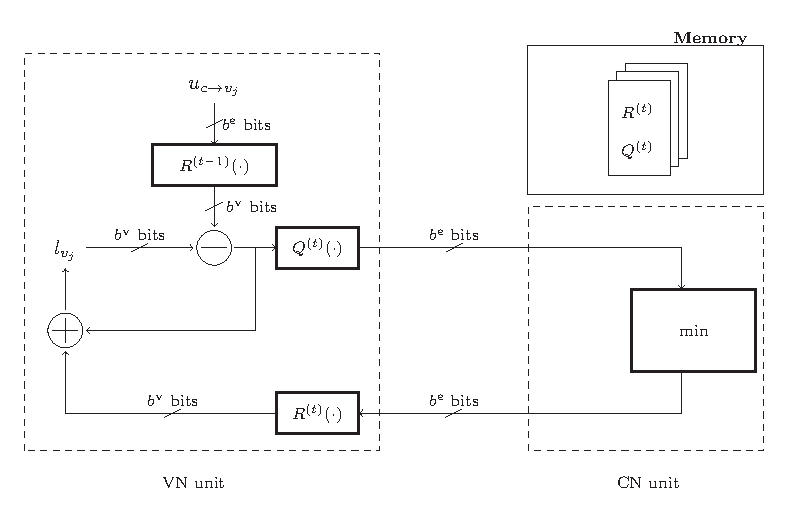
\includegraphics[width=0.7\linewidth]{figures/RCQ_nonlayered.eps}}
\\
  \subfloat[\label{fig: layered_RCQ_str}]{%
        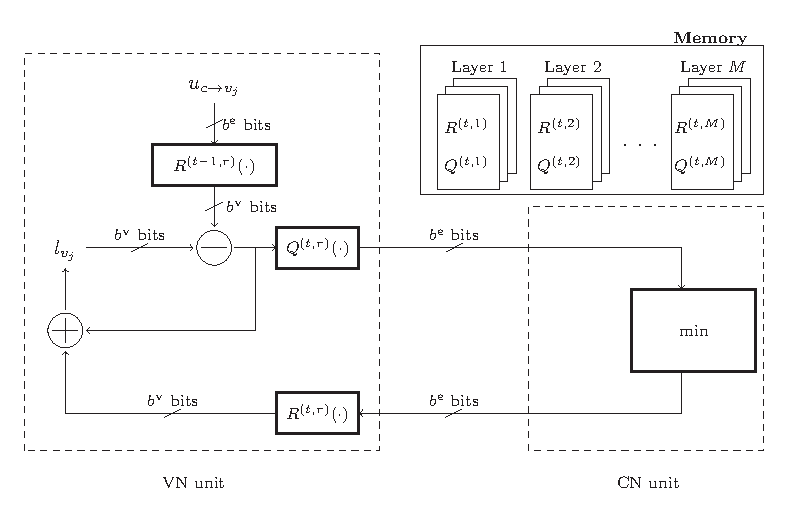
\includegraphics[width=0.7\linewidth]{figures/RCQ_layered.eps}}
  \caption{ Two layered decoders. Fig. (a) uses the same RCQ parameters for each layer as with the  \textit{msRCQ} design for a flooding decoding in \cite{Wang2020-RCQ}. Fig. (b) shows the proposed \textit{layer-specific msRCQ} decoder in \cite{Terrill2021-ec}, which features  separate RCQ parameters for each layer.
  The main difference is that msRCQ decoder uses iteration specific parameters while L-msRCQ decoder considers layer-and-iteration parameters.
  }
\end{figure}

 The msRCQ decoder with a flooding schedule obeys (\ref{equ: Assumption_on_MIM_DDE}) and (\ref{equ: Assumption_on_MIM_DDE2})  because the VN messages to calculate different CN messages have the same distribution. Therefore, it is sufficient for a decoder with a flooding schedule  to use the iteration-specific reconstruction function  $R^{(t)}$ for all external CN messages. However, for a decoder with a layered schedule, the VN messages to calculate CN messages from different layers have different distributions. For the decoder with a layered schedule, $l^{(t)}_{v_j\rightarrow c_i}$ is calculated by:
\begin{align}\label{equ: vari_update_2}
    l^{(t)}_{v_j\rightarrow c_i} = l^{(ch)}_{v_j}&+ \sum_{\{i'|{i'}\in\mathcal{N}(v_j),i'<i\}}u^{(t)}_{c_{i'}\rightarrow v_{j}}+ \sum_{\{i'|{i'}\in\mathcal{N}(v_j),i'>i\}}u^{(t-1)}_{c_{i'}\rightarrow v_{j}},
\end{align}
%We omit $R(\cdot)$ in Eq.(\ref{equ: vari_update_2}) by abuse of notation. 
Unlike a decoder using a flooding schedule, which updates $ l^{(t)}_{v_j\rightarrow c_i}$ only using CN messages in iteration $t-1$, decoders using a layered schedule use messages from both iteration $t-1$ and iteration $t$. The VN messages computed in different layers utilize different proportions of check-to-variable node messages from iterations $t-1$ and $t$.  Since the check-to-variable node messages from different iterations have different reliability distributions, the VN messages from different layers also have different distributions. Therefore \eqref{equ: Assumption_on_MIM_DDE} and \eqref{equ: Assumption_on_MIM_DDE2} no longer hold true, and a single $R^{(t)}(\cdot)$ is insufficient to accurately describe CN messages from different layers. 

In conclusion, the \textit{Representation Mismatch Problem} refers to inappropriately using a single $R^{(t)}$ and single $Q^{(t)}$ for all layers in iteration $t$  of a layered decoding schedule. This issue degrades the decoding performance of layer-scheduled RCQ decoder.  On the other hand, the conventional fixed-point decoders that do not perform coarse non-uniform quantization, such as standard \minsum decoder,  are not affected by the changing the distribution of messages in different layers and hence don't have representation mismatch problem.

\subsection{Layer-Specific RCQ Design}
Based on the analysis in the previous subsection,  $R$ and $Q$ should adapt for the PMF of messages in each layer, in order to solve the representation mismatch problem. This motivates us to propose the layer-specific RCQ decoding structure in this paper, as illustrated in Fig. \ref{fig: layered_RCQ_str}. The key difference between the RCQ decoder and layer-specific RCQ decoder is that layer-specific RCQ designs quantizers and reconstruction mappings for each layer in each iteration.  We use $R^{(t,r)}$ and $Q^{(t,r)}$ to denote the reconstruction mapping and quantizer for decoding iteration $t$ and layer $r$, respectively. 
As illustrated in Fig. \ref{fig: layered_RCQ_str}, layer-specific RCQ specifies $R$ and $Q$ for each layer to handle the issue that messages in different layers have different PMFs. This leads to a significant increase in the required memory because the memory required to store $R^{(t,r)}$ and $Q^{(t,r)}$ is proportional to the product of the number of layers and the number of iterations required for decoding the QC-LDPC code.

Designing $Q^{(t,r)}(\cdot)$ and $R^{(t,r)}(\cdot)$ for layer-specific msRCQ requires the message PMF for each layer in each iteration.  However, HDQ discrete density evolution\cite{Wang2020-RCQ}, which performs density evolution based on ensemble, fails to capture layer-specific information. In this section, we propose a layer-specific HDQ discrete density evolution based on base matrix $H_\text{p}$ of QC-LDPC code. In layer-specific HDQ discrete density evolution, the joint PMF between code bit $X$ and external message $D$ from check/variable nodes are tracked in each layer in each iteration. We use $P^{(t,r)}(X,D^\text{c})$, $X\in\{0,1\}$, $D^\text{c}\in\{0,\ldots,2^{b^\text{e}}-1\}$ to represent the joint PMF between code bit and CN message in layer $m$ and iteration $t$. Similarly, VN messages are denoted by $P^{(t,r)}(X,D^\text{v})$.

\subsubsection{Initialization}
For an AWGN channel with noise variance $\sigma^2$, the LLR of channel observation $y$ is $l=\frac{2}{\sigma^2}y$.
For the msRCQ decoder with bit width $(b^\text{e},b^\text{v})$, the continuous channel LLR input is uniformly quantized into $2^{b^\text{v}}$ regions.  Each quantization region has a true log likelihood ratio, which we refer to as $l_d$, so that we have an alphabet of $b^\text{v}$ real-valued log likelihood ratios ${\mathcal D}^{\text{ch}}=\{l_0,...,l_{2^{b^{\text{v}}}-1}\}$.  Using these values, the joint PMF between the code bit $X$ and channel LLR message $D^{\text{ch}} \in \{0,...,{2^{b^{\text{v}}}-1}\}$ is:
\begin{align}\label{equ: chan_prob}
    P_{XD^{\text{ch}}}(x,d) &= P_D(d) \frac{e^{(1-x)l_d}}{e^{l_d}+1}, ~X\in \{0,1\},\  l_d\in {\mathcal D}^{\text{ch}}\, .
\end{align}
The distribution $P_{XD^{\text{ch}}}(x,d)$ is used for the HDQ discrete density evolution design.  The actual decoder does not use the real-valued likelihoods $l_d$ but rather uses $b^{\text{v}}$-bit channel LLRs obtained by uniformly quantizing continuous channel LLR values.
\subsubsection{Variable Nodes PMF Calculation}
Given a base matrix $H_\text{p}$, with entry $H_\text{p}(r,c)$ at row $r$ and column $c$, define the sets of active rows $\mathcal{R}(c)$ for a specified column $c$ and active columns $ \mathcal{C}(r)$ for a specified row $r$ as follows:
\begin{align}
\mathcal{R}(c) = \{r| H_\text{p}(r,c)\neq0\}
,\quad 
\mathcal{C}(r)= \{c| H_\text{p}(r,c)\neq0\}.
\end{align}
In iteration $t$ and layer $r$, consider the joint PMF between a code bit $X$ corresponding to a VN in the circulant $H_\text{p}(r,c)$ and the vector $\mathbf{D}$, which includes the channel message $D^{\text{ch}}$ for $X$ and the check node messages $D^{\text{c}}$ incident to that VN.  This PMF is calculated by:
\begin{align}
\begin{split}
        P_\text{v}^{(t,r,c)}(X,\mathbf{D})&=P(X,D^{\text{ch}})\boxdot\left(\boxdot_{\substack{k\in\mathcal{R}(c) \\ k<r}}P^{(t,k)}(X,D^{\text{c}})\right) \\&\boxdot\left(\boxdot_{\substack{k\in\mathcal{R}(c) \\ k>r}}P^{(t-1,k)}(X,D^{\text{c}})\right), 
\end{split}
    \label{eq: vari_update}
\end{align}
$\boxdot$ is defined as follows: 
\begin{align}
    P(x,[d_1,d_2])&=P({X_1,D_1})\boxdot P({X_2,D_2})\\&\triangleq\frac{1}{P_X(x)}P_{X_1D_1}(x,d_1)P_{X_2D_2}(x,d_2),
\end{align}
% Unlike HDQ-DDE, which takes the same PMF to all incoming messages from different layers ( (12) in \cite{Wang2020-RCQ}), Eq.(\Ref{eq: vari_update}) utilizes layer-specific PMF. 
$ x\in\{0,1\},~d_1,d_2\in\{0,\ldots,2^{b^\mathrm{e}}-1\}$. When $|\mathcal{R}(c)|$ is large, the alphabet ${\mathcal D}$ of possible input message vectors $\mathbf{D}$ is large with $|{\mathcal D}|=2^{b^\mathrm{v}+(|\mathcal{R}(c)|-1)b^\mathrm{e}}$.  To manage the complexity of HDQ discrete density evolution, message vectors $\mathbf{D}$ with similar log likelihoods are clustered via  one-step-annealing as in \cite{Wang2020-RCQ} for (\Ref{eq: vari_update}).

The layer-specific msRCQ decoder uses layer-specific parameters, and for each layer the marginal distribution on the computed variable node messages will be distinct. The marginal distribution used by HDQ at layer $r$ is computed as follows:
\begin{align}\label{eq: vari_total}
    \Tilde{P}_\text{v}^{(t,r)} = \left\{\frac{1}{|\mathcal{C}(r)|}P_\text{v}^{(t,r,c)}(X,\mathbf{D})\mid c\in\mathcal{C}(r)\right\}\,
\end{align}
 where ${P}^{(t,r)}(X,D^v)$ and $Q^{(t,r)}(\cdot)$ can be obtained by quantizing  $\Tilde{P}_\text{v}^{(t,r)}$ using HDQ:
\begin{align}\label{eq: vari_hdq}
    \left[P^{(t,r)}(X,D^{\text{v}}),Q^{(t,r)}(\cdot) \right] = \texttt{HDQ}\left(\Tilde{P}_\text{v}^{(t,r)}, 2^{b^\mathrm{e}}\right),
\end{align}
where \texttt{HDQ} is defined as a function that realizes $b^e$-bit HDQ on  $\Tilde{P}_\text{v}^{(t,r)}$ and generates $P^{(t,r)}(X,D^{\text{v}})$ and $Q^{(t,r)}$ as outputs. Note that (33) and (34) realize implicit message alignment in \cite{Stark2021-ai} such that the internal messages from  any  $c\in\mathcal{C}(r)$  use same set of thresholds for quantization and the same external messages from any $c\in\mathcal{C}(r)$ have same LLR interpretations, regardless of node degree.

\subsubsection{Check Nodes PMF Calculation}
Let $l^{(t,r)}_\text{v}{(d)}$ be the LLR of external VN message $d$ in layer $r$ and iteration $t$.  As an LLR, this CN input  $l^{(t,r)}_\text{v}{(d)}$ has the following meaning: 
\begin{align}
    l_\text{v}^{(t,r)}(d) = \log \frac{P_{XD^\text{v}}^{(t,r)}(0,d)}{P_{XD^\text{v}}^{(t,r)}(1,d)},\quad d=0,...,2^{b^{e}}-1.
\end{align}
Given input messages $d_1,d_2\in {\mathcal D}^\text{v}$, the CN min operation produces the following output:
\begin{align}\label{equ: label_min}
\begin{split}
     l_{\text{MS}}^{\text{out}} =&\min\left(|l_\text{v}^{(t,r)}(d_1)|,|l_\text{v}^{(t,r)}(d_2))|\right)\\&\times \text{sgn}(l_\text{v}^{(t,r)}(d_1))\times\text{sgn}(l_\text{v}^{(t,r)}(d_2)). 
\end{split}
\end{align}
Under the symmetry assumption, there is a $d^{\text{out}}\in {\mathcal D}^\text{v}$ that has the LLR computed as $l_{\text{MS}}^{\text{out}}$:
\begin{align}\label{equ: label_min_2}
    l_{\text{MS}}^{\text{out}}=\log \frac{P^{(t,r)}_{XD^\text{v}}(0,d^{\text{out}})}{P^{(t,r)}_{XD^\text{v}}(1,d^{\text{out}})}.
\end{align}
At the check node output, $l_{MS}^{out}$ will be assigned the label $d^{out}\in {\mathcal D}^v$ that satisfies \eqref{equ: label_min_2}.  However, the LLR meaning associated with that $d^{out}$ must be adjusted. 

Define the follow function: 
\begin{align}\label{equ: label-min}
    d^\text{out} = \texttt{MS}(d_1,d_2),
\end{align}
 where $d^{\text{out}},d_1,d_2\in \mathcal{D}^\mathrm{v} $. \eqref{equ: label-min} holds if and only if \eqref{equ: label_min} and \eqref{equ: label_min_2} and are both satisfied.


Define the binary operation $\circledast$ by:
\begin{align}
          \Tilde{P}_{XD}(x,d) &= P(X_1,D_1)\circledast P(X_2,D_2)\\&\triangleq\sum_{\substack{d_1,d_2:\texttt{MS}(d_1,d_2)=d \\ x_1,x_2: x_1\bigoplus x_2 = x}}P_{X_1D_1}(x_1,d_1)P_{X_2D_2}(x_2,d_2)\label{equ: msrcq-c}.
\end{align}


%To obtain the new LLR for $d^{out}$, 
The joint PMF between code bit and external CN message in layer $r$ and iteration $t$ can be updated by:
\begin{align}
 P^{(t,r)}(X,D^\text{c}) &=P^{(t,r)}(X,D^\text{v})\circledast ...\circledast P^{(t,r)}(X,D^\text{v})\\&\triangleq P^{(t,r)}(X,D^\text{v})^{\circledast(|\mathcal{C}(r)|-1)}. \label{equ: check_opt_prob2}
\end{align}
$R^{(t,r)}(\cdot)$ can be directly computed using $P^{(t,r)}(X,D^\text{c})$:
\begin{align}
        R^{(t,r)}(d) = \log \frac{P_{XD^\text{c}}^{(t,r)}(0,d)}{p_{XD^\text{c}}^{(t,r)}(1,d)},~d\in\{0,...,2^{b^\text{e}}-1\}.
        \label{eq: r_v}
\end{align}

\subsection{Threshold}
The threshold of a layer-specific RCQ decoder given a base matrix with $M$ layers and  maximum number of decoding iterations $I_T$ is defined as: 
\begin{align}
    \frac{E_b}{N_o}^*=\inf \left\{\frac{E_b}{N_o}:  I^{(I_T,r)}\left(\frac{E_b}{N_o}\right)> 1-\epsilon,\forall  r\in[1,M] \right\}.
\end{align}

\begin{figure}[htp] 
    \centering
  \subfloat[Decoders with floating point messages\label{fig: 80211_1}]{%
       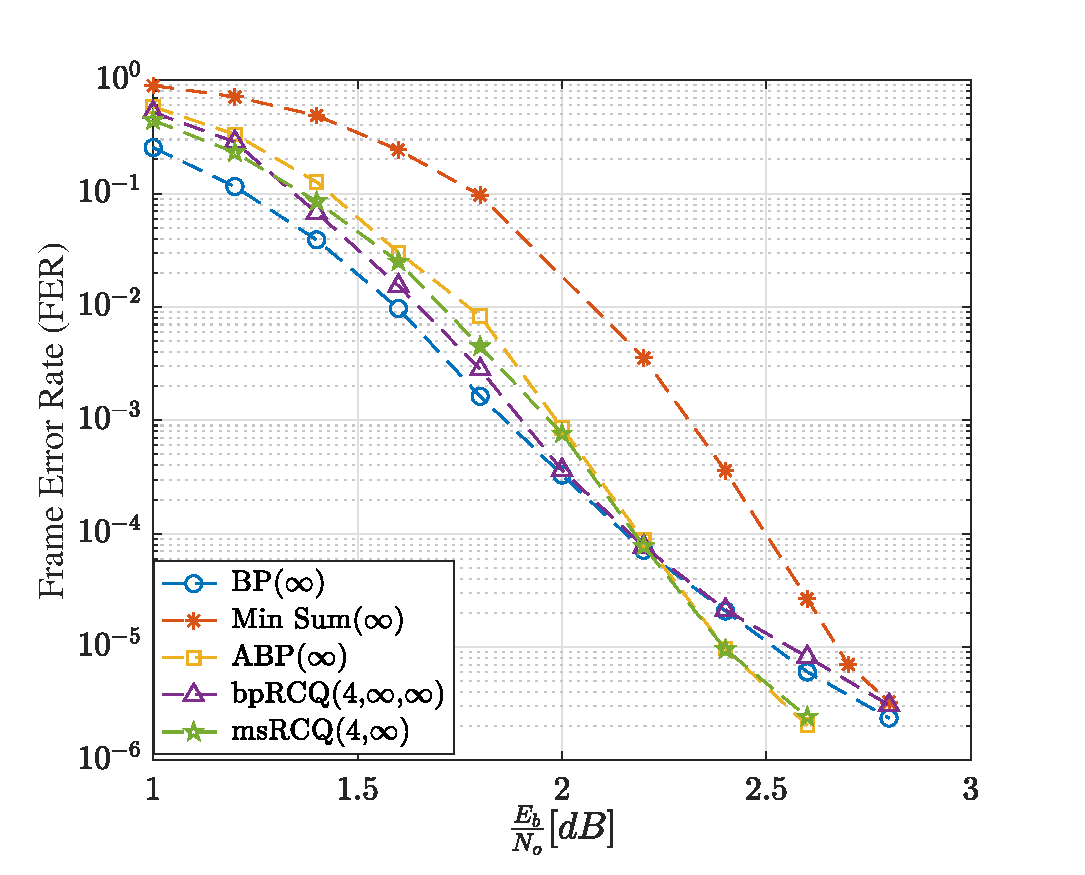
\includegraphics[width=0.5\linewidth]{figures/80211_fig1.eps}}
\\
  \subfloat[Decoders with fixed point messages\label{fig: 80211_3}]{%
        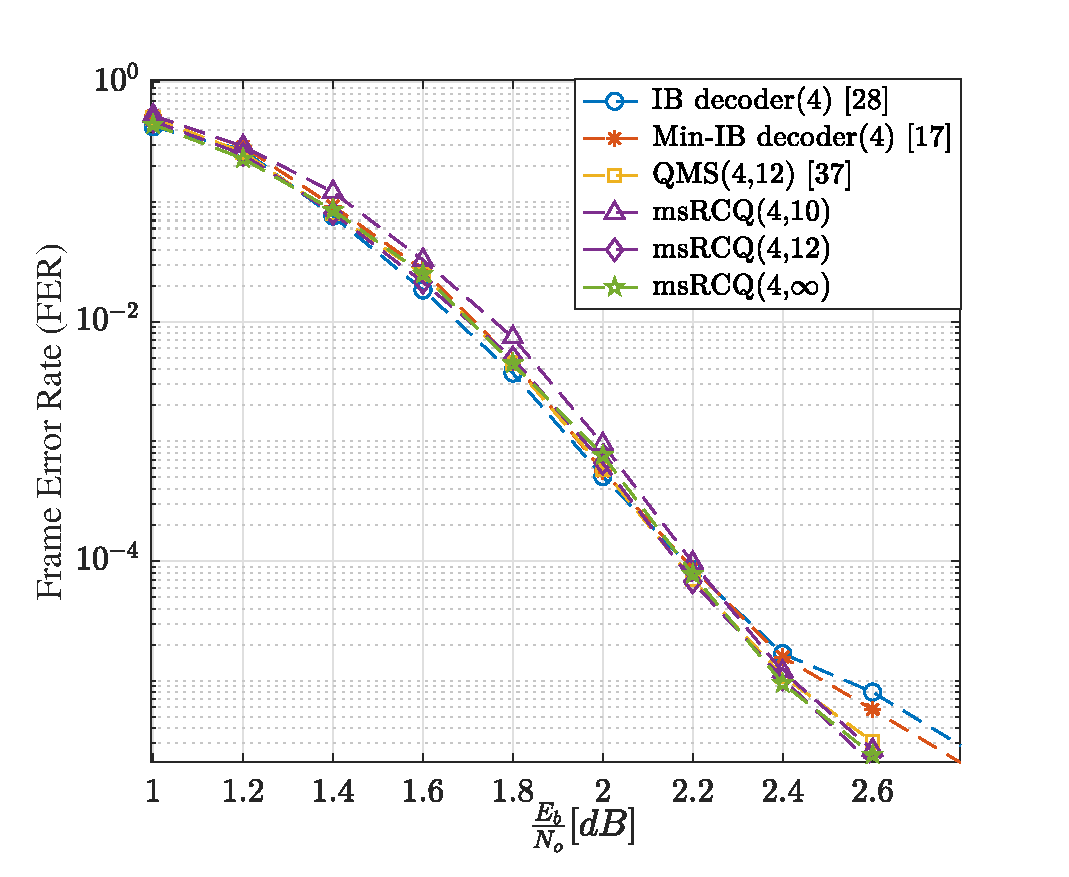
\includegraphics[width=0.5\linewidth]{figures/80211_fig3.eps}}
  \caption{Fig. (a): FER performance of 4-bit msRCQ and bpRCQ decoders with floating point message representations use at the VNs.  Fig. (b):FER performance of fixed point 4-bit msRCQ decoders, compared with other non-uniform quantization decoders. }
\end{figure}

\section{Simulation Result and Discussion}\label{sec: simulation result}
This section presents RCQ and layer-specific RCQ decoder designs for two example LDPC codes and compares their FER performance  with existing conventional decoders such as BP, \minsum, and state-of-the-art non-uniform decoders, such as an IB decoder. All decoders are simulated using the AWGN channel, and at least 100 frame errors are collected for each point.  We also compare hardware requirements for an example LDPC code.
\subsection{IEEE 802.11 Standard LDPC Code}
We first investigate the FER performance of RCQ decoders with a flooding schedule using an IEEE 802.11n standard LDPC code taken from \cite{80211spec}. This code has $n=1296$, $k=648$, and the edge distribution is:
\begin{align}
    \lambda(x) &= 0.2588x+0.3140x^2+0.0465x^3+0.3837x^{10}, \\
    \rho(x) &= 0.8140x^6 +0.1860 x^7.
\end{align}
The maximum number of decoding iterations was set to 50.

Fig. \ref{fig: 80211_1} shows the FER curves of  4-bit bpRCQ and msRCQ decoder with floating-point internal messages, i.e., {bpRCQ}(4,$\infty$,$\infty$) and {msRCQ}(4,$\infty$), respectively . The notation of $\infty$ represents floating-point message representation. Denote floating point BP nad Min Sum by BP($\infty$) and Min Sum($
\infty$), respectively.  The 4-bit bpRCQ decoder has at most 0.1 $dB$ degradation compared with the floating-point BP decoder, and outperforms floating-point BP at high $\frac{E_b}{N_o}$.  The 4-bit msRCQ performs better than conventional \minsum and even surpasses BP at high $\frac{E_b}{N_o}$. The lower error floor of msRCQ decoder as compared to standard BP follows from the slower message magnitude convergence rate as compared to standard BP. This is similar to improved error floors achieved by the averaged BP (ABP) [35], which  decreases the rate of increase of message magnitudes by averaging the posteriors  $l_v^{(t)}$ in consecutive iterations. As shown in Fig. \ref{fig: 80211_1}, ABP also delivers a lower error floor than standard BP.

 The slow magnitude convergence rate of msRCQ decoder can be explained as follows.  For conventional \minsum decoder, the magnitude of each check node message is always equal to the magnitude of an input variable node message for that CN.  This is not true for the msRCQ decoder. msRCQ compares the relative LLR meanings of input messages and returns an external message by implementing the min operation. However, the external message is then reconstructed at the VN to an internal message magnitude that is in general different from the message magnitudes that were received by the neighboring CN. 

 For the example of a degree-3 CN, \eqref{equ: ave_msrcq} computes the likelihood associated with a message $l_t$ that is outputted from the min operation applied to the other two input messages indexed by $i$ and $j$:
\begin{align}\label{equ: ave_msrcq}
    l_{t}&=\log\frac{\sum_{\{(i,j)|t=MS(i,j)\}}P(0,i)P(0,j)+P(1,i)P(1,j)}{\sum_{\{(i,j)|t=MS(i,j)\}}P(1,i)P(0,j)+P(0,i)P(1,j)}. 
\end{align}
Note that the boxplus operation is computed as follows :
\begin{align}
   l_i\boxplus l_j &=\log \frac{P(0,i)P(0,j)+P(1,i)P(1,j)}{P(0,i)P(1,j)+P(1,i)P(0,j)}\label{equ: box_plus_p}.
\end{align}
MinSum is an approximation to the boxplus operation, and boxplus produces a range of message values for edges that would share the same MinSum value $MS(i,j)$. 
Comparing with \eqref{equ: box_plus_p}, it can be seen that \eqref{equ: ave_msrcq} applies the boxplus operation to the probability of the group of messages that share same value for $MS(i,j)$. Applying the boxplus operation to the {\em group} of messages produces a value that lies between the extremes of the messages produced by individual boxplus operations.  This grouping process lowers the maximum output magnitude and therefore decreases the message magnitude growth rate in an iterative decoding process. 
\begin{figure}
	\centering
	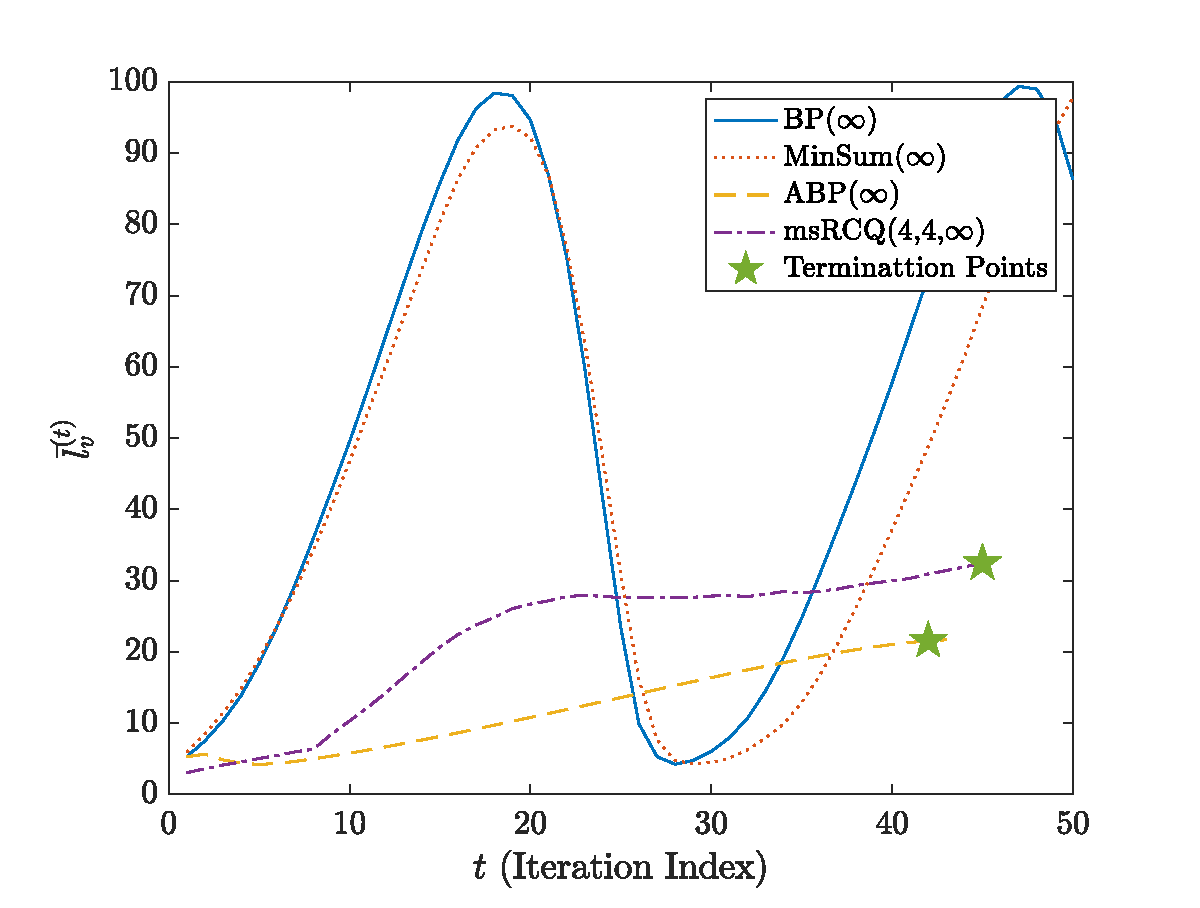
\includegraphics[width=0.5\linewidth]{figures/80211_fig2.eps}
	\caption{Average magnitudes of $l^{(t)}_v$ vs. iteration for BP, ABP, \minsum and msRCQ for Fig.  6a simulation at  $\frac{E_b}{N_o}=2.6$ dB.
	}
	\label{fig: 80211_2}
\end{figure}
As noted in \cite{ABP}, a possible indicator of the emergence of error trapping sets may be a sudden magnitude change in the values of certain variable node messages, or fast convergence to an unreliable estimate. Therefore, slowing down the convergence rate of VN messages can decrease the frequency of trapping set events. Both msRCQ decoder and A-BP in \cite{ABP} reduce the the convergence rate of VN messages and hence deliver a lower error floor. However, A-BP requires extra computations to calculate the average message. On the other hand, the averaging process of msRCQ (i.e., \ref{equ: ave_msrcq}) is inherent in $R(\cdot)$ and does not require additional complexity. 

The effect of averaging can be seen in Fig. \ref{fig: 80211_2}, which gives the average magnitude of $l^{(t)}_v$ for four decoders with a noise-corrupted all-zero codeword at $\frac{E_b}{N_o}=2.6$ dB as the input. The oscillation pattern of the BP decoder has been reported and discussed in \cite{ABP}.  As shown in Fig. \ref{fig: 80211_1}, ABP also outperforms belief propagation when $\frac{E_b}{N_o}$ is high. 
The oscillation occurs as errors alternate between the variable nodes that comprise the trapping set and their complement.
Note that ABP requires extra computations to calculate the average message. However, the implicit averaging process of msRCQ (i.e., \eqref{equ: ave_msrcq}) is inherent in $R(\cdot)$. 

Fig. \ref{fig: 80211_3} compares msRCQ(4,10) with other non-uniform quantization LDPC decoders. Simulation results show that both IB\cite{Lewandowsky2018-IBRegular} and Min-IB\cite{Meidlinger2017-MINIBIRR} decoders exhibit an error floor after $2.40dB$. The MIM-QMS\cite{kang2020generalized} decoder has a similar decoding structure to msRCQ. Note that MIM-QMS requires the determination of the internal bit width used by the VNs before designing quantization and reconstruction parameters, so reducing the bit width of VNs requires another design cycle. 
In contrast, for the purposes of HDQ discrete density evolution design process, msRCQ assumes that the internal VN  messages are real-valued. This assumption is an approximation since the internal VN messages will have finite precision in practical implementations. During actual decoding, the reconstruction operation $R(\cdot)$ produces a high-precision representation for use in computations at the VN. We found that assuming real-valued internal messages in the design process introduces negligible loss for practical internal message sizes while greatly simplifying the design. Our simulation results in \ref{fig: 80211_3} confirm that high precision internal messages have FER performance that is very close to real-valued internal messages.
Actually, for the msRCQ, it is sufficient to have a simple clipping module at variable node, because all reconstructed values are fixed point messages. 
The RCQ decoder has more efficient memory usage than LUT-based decoders. For the investigated non-uniform LDPC code, 4-bit IB and 4-bit Min-IB require 14.43k and 10.24k bits, respectively, for storing LUTs per iteration, whereas msRCQ(4,12) and msRCQ(4,10) require 165 bits and 135 bits only.   
\begin{figure}[hp] 
    \centering
  \subfloat[\label{fig: 8k_FER}]{%
       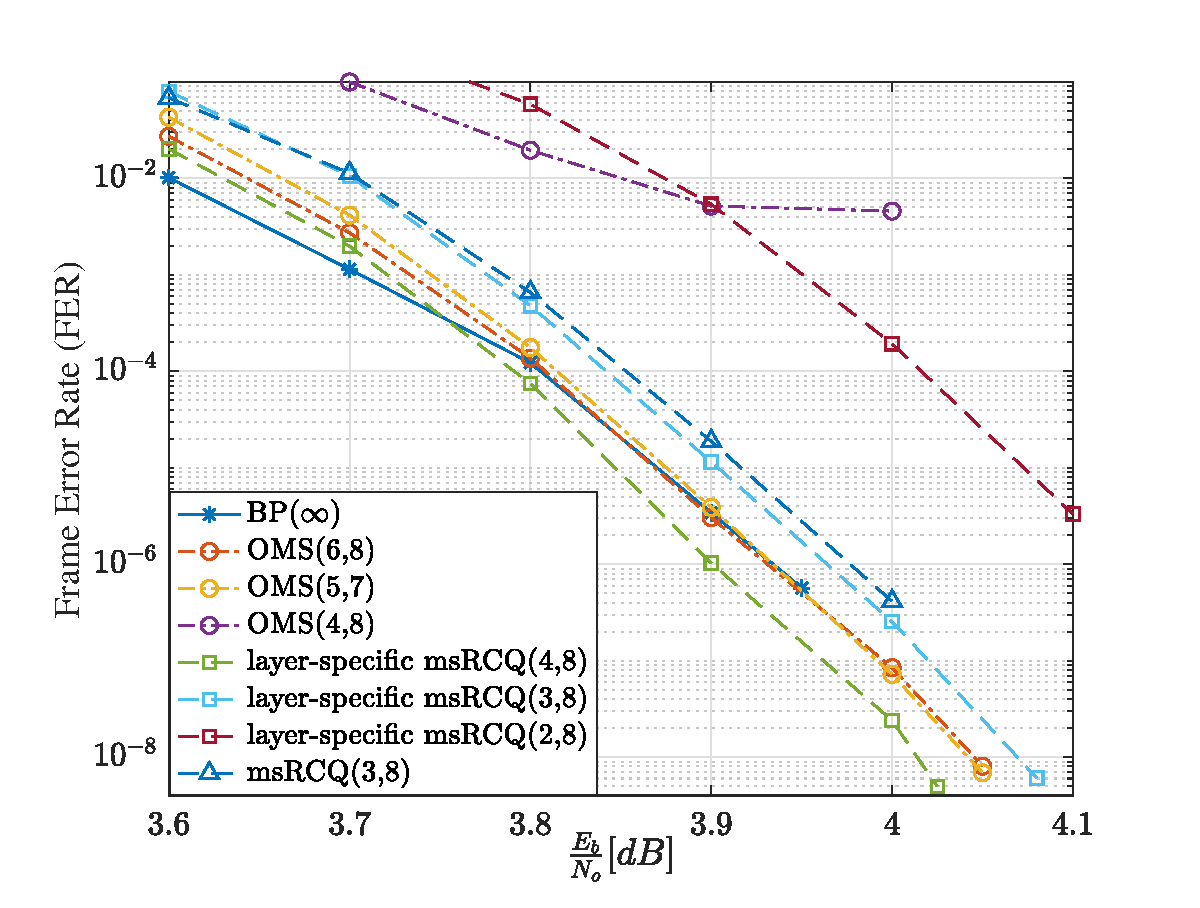
\includegraphics[width=0.5\linewidth]{figures/8k_fer3.eps}}
\\
  \subfloat[\label{fig: 8k_ADIT}]{%
        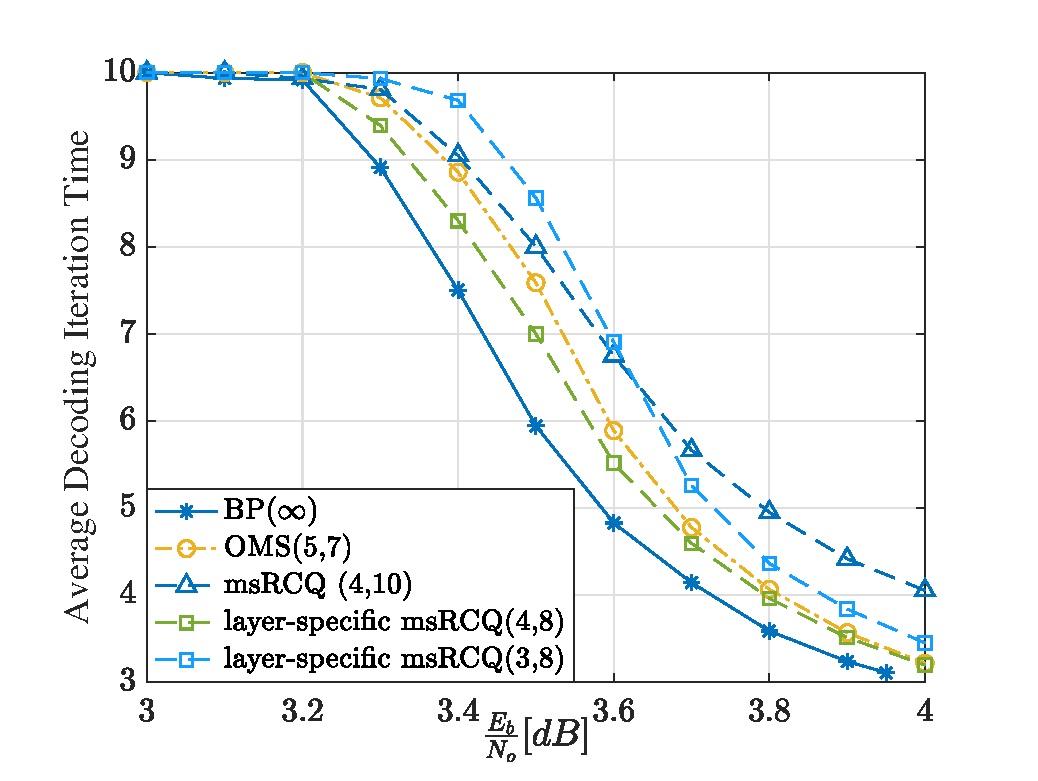
\includegraphics[width=0.5\linewidth]{figures/8K_ADIT.eps}}
  \caption{Fig. (a): FER performance of fixed point L-msRCQ decoders for (9472, 8192) LDPC code.  Fig.  (b): FER performance of fixed point L-msRCQ decoders for (9472, 8192) LDPC code. } \label{fig: 8k_performance}
\end{figure}

\subsection{(9472, 8192) QC-LDPC code}
In this subsection we consider a rate-0.8649 quasi-regular LDPC code, with all VNs having degree 4 and CNs having degree 29 and 30, as might be used in a flash memory controller. We study this (9472, 8192) QC-LDPC code using various decoders with a \textit{layered schedule}. The layer number of the investigated LDPC code is 10.  

Fig. \ref{fig: 8k_FER} shows the FER curves of various decoders. The maximum number of decoding iterations of all studied decoders is 10. The layer-specific msRCQ(4,8) outperforms msRCQ(4,10) by 0.04 dB, which shows the benefit of optimizing layer and iteration specific RCQ parameters.  
The layer-specific msRCQ(3,8) delivers similar decoding performance to msRCQ(4,10). The decoding performance of 2-bit layer-specific msRCQ has a 0.2 dB degradation compared with the 4-bit  layer-specific msRCQ decoder. 
Given that  $I_T=10$, the thresholds of the investigated LDPC code under 4-bits msRCQ and 2-4 bit LS-msRCQ decoders  are 3.58 dB, 3.67 dN,  3.46 dB  and 3.40 dB, respectively. 
Fig. \ref{fig: 8k_FER} also shows a fixed point offset \minsum (OMS) decoder with offset factor 0.5. At a FER of $10^{-8}$, OMS(6,8) and OMS(5,7) outperform layer-specific msRCQ(3,8) by 0.02 dB, yet are inferior to layer-specific msRCQ(4,8) by 0.02 dB.  
\begin{table*}[t]
    \centering
    \caption{\label{tab: hardware_usage} Hardware Usage of Various Decoding Structure for (9472,8192) QC-LDPC Code }
    \begin{tabular}{|c|c|c|c|c|}
    \hline
    Decoding Structure & LUTs                       & Registers                  & BRAMS                        & Routed Nets                \\ \hline
    OMS(5,7) (baseline)          & 21127                      & 12966                     & 17                    & 29202                      \\ \hline
    layer-specific RCQ(4,8)           & 20355(\textcolor{mygreen}{$\downarrow 3.6\%$} ) & 13967(\textcolor{red}{$\uparrow 7.0\%$}) & 17.5(\textcolor{red}{$\uparrow .03\%$}) & 28916(\textcolor{mygreen}{$\downarrow 1\%$}) \\ \hline
    layer-specific RCQ(3,8)           & 17865(\textcolor{mygreen}{$\downarrow 15.4\%$}) & 12098(\textcolor{mygreen}{$\downarrow 6.7\%$}) & 17(\textcolor{blue}{$-$})                &  25332\textcolor{mygreen}{($\downarrow 13.3\%$}) \\ \hline
    \end{tabular}
    \end{table*}
Fig. \ref{fig: 8k_ADIT} shows the average decoding iteration times for some of the decoders studied in Fig. \ref{fig: 8k_FER}. At high $\frac{E_b}{N_o}$, the msRCQ(4,10) decoder requires the largest average number of iterations to complete decoding. On the other hand, layer-specific msRCQ(4,8) has a similar decoding iteration time to OMS(5,7) and BP($\infty$) in this region. Layer-specific msRCQ(3,8) requires a slightly higher average number of iterations than layer-specific msRCQ(4,8) and OMS(5,7). 
%The decoding iteration time of OMS(6,8), L-msRCQ(4,8) and L-msRCQ(3,8) are 3.13, 3.20 and 3.44, respectively.

We implemented OMS and layer-specific msRCQ decoders with different bit widths on the programmable logic of a Xilinx Zynq UltraScale+ MPSoC device for comparison. Each design meets timing with a 500 MHz clock. The broadcast method described in \cite{Terrill2021-ec} is used for RCQ design. 
Table \ref{tab: hardware_usage_1} summarizes the hardware usage of each decoder. 
Simulation result shows that layer-specific msRCQ(4,8) has a similar hardware usage with OMS(5,7), and layer-specific msRCQ(3,8) has more than a $10\%$ reduction in LUTs and routed nets and more than a $6\%$ reduction in registers, compared with OMS(5,7).

\section{Conclusion}\label{sec: conclusion}
This chapter investigates the decoding performance and resource usage of RCQ decoders. For decoders using the flooding schedule, simulation results on an IEEE 802.11 LDPC code show that a 4-bit msRCQ decoder has a better decoding performance than LUT based decoders, such as IB decoders or Min-IB decoders, with significantly fewer parameters to be stored. It also surpasses belief propagation in the high $\frac{E_b}{N_o}$ region because a slower message convergence rate avoids trapping sets. For decoders using the layered schedule, conventional RCQ design leads to a degradation of FER performance and higher average decoding iteration time. Designing a layer-specific RCQ decoder, which updates parameters in each layer and iteration, improves the performance of a conventional RCQ decoder under a layered schedule.
Layer-specific HDQ discrete density evolution is proposed to design parameters for RCQ decoders with a layered schedule. FPGA implementations of RCQ decoders are used to compare the resource requirements of the decoders studied in this paper. 
Simulation results for a (9472, 8192) QC LDPC code show that a layer-specific \minsum RCQ decoder with 3-bit messages achieves a more than $10\%$ reduction in LUTs and routed nets and a more than $6\%$ register reduction while maintaining comparable decoding performance, compared to a 5-bit offset \minsum~decoder.

\chapter{RCQ LDPC Decoding with Degree-Specific Neural Edge Weights} \label{cpt: W_RCQ}
\section{Introduction}
Low-Density Parity-Check  (LDPC) codes \cite{GallagerPhD1963} have been implemented broadly, including in NAND flash systems and wireless communication systems. In practice, decoders for LDPC codes with low message bit widths are desired when considering the limited hardware resources on the field-programmable gate arrays (FPGAs) or application-specific integrated circuits (ASICs), such as area, routing capabilities, and power utilization. Unfortunately, low-bitwidth decoders with uniform quantizers typically suffer a large degradation in decoding performance\cite{Lee2005-RFQThorpe}. Recently, the non-uniformly quantized decoders  \cite{Planjery2012-FAID,Xiao2020-sb, Lewandowsky2018-IB,Stark2018-IBMA,Stark2019-IBPBRL,Lee2005-RFQThorpe,He2019-RFQCai, Wang2020-kh,terrill2021fpga,wang2022TCOMRCQ}  have shown to deliver excellent performance with very low message precision. One promising decoding paradigm is called reconstruction-computation-quantization (RCQ) decoder \cite{Wang2020-kh,terrill2021fpga,wang2022TCOMRCQ}. 
 
The node operation in an RCQ decoder involves a reconstruction function that allows high-precision message computation and a quantization function that allows low-precision message passing between nodes. Specifically, the reconstruction function, equivalent to a dequantizer,  maps the low-bitwidth messages received by a node to  high-bitwidth messages for computation. The quantization function quantizes the calculated high-bitwidth messages to low-bitwidth messages that will be sent to its neighbor nodes. 
 As shown in \cite{terrill2021fpga}, the 4-bit  layer-scheduled RCQ decoder can have a better decoding performance than the 6-bit uniformly quantized offset MinSum (OMS) decoder. 

 The excellent decoding performance of RCQ decoder comes from its dynamic quantizers and dequantizers that are updated in each layer and each iteration. However, for practical consideration, the dynamic quantizers and dequantizers mean more look-up tables (LUTs). What's worse, the LUTs required for storing quantizers and dequantizers may offset the LUTs saved by using low bit width to pass messages.  As reported in \cite{wang2022TCOMRCQ}, the 4-bit RCQ decoder has a similar LUT usage to the 5-bit OMS decoder for a (9472,8192) LDPC code. 

Recently, numerous works have been focused on enhancing the performance of message-passing decoders with the help of neural networks (NNs) \cite{Nachmani2016-bs,Lugosch2017-ed,Nachmani2017-qq,Nachmani2018-ra,Liang2018-lw,Wu2018-zr,Lugosch2018-gu,Lyu2018-nz,Xiao2019-kj,Deng2019-cf,Abotabl2019-wt,Buchberger2020-pf,Wang2020-fb,Lian2019-jh,nguyen2021neural}. 
%The neural network is created by unfolding the message passing operations of each decoding iteration \cite{Nachmani2016-bs}.
%Each decoding iteration is unfolded into two hidden layers which represent check node processing layer and variable node processing layer and each neuron represents a variable-to-check message or a check-to-variable message. 
Nachmani \textit{et al.} in \cite{Nachmani2016-bs} propose a  neural belief propagation (N-BP) decoder that assigns NN-learned multiplicative weights to the BP messages.
Nachmani \textit{et al.} and Lugosch \textit{et al.} in \cite{Nachmani2018-ra, Lugosch2017-ed,Nachmani2016-bs} assign dynamic weights to the messages in  normalized MinSum (NMS) and OMS decoder and propose the Neural NMS (N-NMS) and Neural OMS (N-OMS) decoder, respectively.


For the above neural decoders, each check-to-variable message and/or each variable-to-check message is assigned a distinct weight in each iteration.
These neural decoders are impractical for long-blocklength LDPC codes because the number of required parameters is proportional to the number of edges in the Tanner graph corresponding to the parity check matrix.  
One solution is to share the weights across iterations or edges in the Tanner graph, like in \cite{Nachmani2017-qq,Wang2020-fb,Abotabl2019-wt, Lian2019-jh}. However, these simple weight-sharing methods sacrifice decoding performance in different ways.
Besides, the precursor works of literature are mainly focused on the short-blocklength codes ($n<2000$), which may have resulted from the fact that the required memory for training neural decoders with long block lengths by using popular deep learning research platforms, such as Pytorch, is larger than the computation resources of the researchers. 
However, as demonstrated in \cite{Abotabl2019-wt,wang2021ISTC}, it is possible to train neural decoders by only using CPUs on personal computers for very long-blocklength codes if resources are handled more efficiently. 

\subsection{Contribution}
This paper combines the recent neural decoding with RCQ decoding paradigm and proposes a weighted RCQ (W-RCQ) decoder. Unlike RCQ decoder, whose quantizers/dequantizers  change in each layer and iteration, the W-RCQ decoder limits the number of quantizer and dequantizer pairs to a very small number, for example, three. However, the W-RCQ decoder weights check-to-variable node messages using dynamic parameters optimized via a quantized NN (QNN). The proposed W-RCQ decoder uses fewer parameters than the RCQ decoder, requiring much fewer LUTs. 

The novelties and contributions of this paper are summarized as follows:  
\begin{itemize}
    \item \textit{Posterior Joint Training Method.} This paper identifies the gradient explosion issue when training neural LDPC decoders. A posterior joint training method is proposed in this paper to address the gradient explosion problem. Simulation results show that posterior joint training delivers a better decoding performance than simply clipping large-magnitude gradients to some threshold value.
     \item \textit{Node-Degree-Based Weight Sharing}. 
     This paper illustrates that the weight values of the N-NMS decoder are strongly related to check node degree, variable node degree, and iteration index. As a result, this paper proposes node-degree-based weight-sharing schemes that assign the same weight to the edges with the same check and/or variable node degree.
     \item \textit{Neural-2D-MinSum decoder}. By employing the node-degree-based weight sharing  on the N-NMS and N-OMS decoder, this paper proposes the N-2D-NMS decoder and N-2D-OMS decoder. \emph{2D} represents for 2-dimensional and implies that the weights are shared based on two dimensions, i.e., check node degree and variable node degree.
     Simulation results on the (16200,7200) DVBS-2 LDPC code show that the N-2D-NMS decoder can achieve same decoding performance as N-NMS decoder. 
    \item  \textit{W-RCQ Decoder.} This paper proposes the W-RCQ decoding paradigm.  Our simulation result for a (9472,8192) LDPC code on a field-programmable gate array (FPGA) device shows that the 4-bit W-RCQ decoder delivers comparable FER performance but with much fewer hardware resources, compared with the 4-bit RCQ decoder and the 6-bit offset MinSum decoder.
\end{itemize}

\subsection{Organization}

The remainder of this paper is organized as follows: Section \ref{sec: effi_NNMS} derives the gradients for a flooding-scheduled N-NMS decoder and shows that the memory to calculate the gradients can be saved by storing the forward messages compactly. The derivations enable one to build and train the NNs for the neural decoders using programmable languages such as C++. The compact message format saves the required memory for training NNs. This section also describes the posterior joint training method that addresses the gradient explosion issue. Section \ref{sec: N-2D-NMS} illustrates the relationship between neural weights of N-NMS decoder and node degree. The node-degree-based weight-sharing scheme is presented in this section. This section also gives neural-2D-MinSum decoders. Section \ref{sec: W-RCQ} gives the W-RCQ decoding structure and describes how to train W-RCQ  parameters via a QNN. The simulation results are presented in Section \ref{sec: Simulation}, and Section \ref{sec: conclusion_c2} concludes our work. 

\section{Training Neural MinSum Decoders for Long Blocklength Codes}\label{sec: effi_NNMS}
For the neural network corresponding to a neural LDPC decoder, the number of neurons in each hidden layer equals the number of edges in the Tanner graph corresponded to the parity check matrix  \cite{Nachmani2016-bs}. For the popular NN platforms, such as PyTorch, each neuron requires a data structure that stores the value of the neuron, the gradient of the neuron, the connection of this neuron with other neurons, and so on. Hence, there is a huge memory requirement for PyTorch to train the neural decoders for long-blocklength LDPC codes. (difficult for researchers with limited resources usage)


The data structure used in PyTorch is useful and convenient for conventional deep neural network tasks but redundant to the neural LDPC decoders. One reason is that the neuron connections between hidden layers are repetitive and can be interpreted by the parity check matrix.
%As a result, the neural network can perform the back propagation by only knowing the parity check matrix, rather than recording how each neurons are connected between two hidden layers. 
This immediately reduces the required memory.  
This section uses N-NMS decoder as an example to show that the memory required to calculate gradients of neural MinSum decoders can be further reduced by storing the messages in forward propagation compactly.

\subsection{Forward Propagation of N-NMS Decoder}
Let $H\in\mathbb{F}_2^{n\times k}$ be the parity check matrix of an $(n,k)$ binary LDPC code, where $n$ is the codeword length and $k$ is dataword length. Denote $i^{th}$ variable node and $j^{th}$ check node by $v_i$ and $c_j$, respectively. 
%In each iteration, an NMS decoder uses the same constant value to scale all  check-to-variable node messages, whereas an N-NMS decoder assigns distinct multiplicative parameters for each check-to-variable message in each iteration.  
For the flooding-scheduled decoder, in the $t^{th}$ decoding iteration, N-NMS decoder updates the check-to-variable (C2V) message, $u^{(t)}_{c_j \rightarrow v_i}$, by: 
\begin{align}
     u^{(t)}_{c_i\rightarrow v_j} &= \beta^{(t)}_{(c_i,v_j)} \times  \prod_{v_{j'}\in \mathcal{N}(c_i)\setminus\{v_j\}} \text{sgn}\left(l^{(t-1)}_{v_{j'}\rightarrow c_{i}}\right)  \times  \min_{v_{j'}\in \mathcal{N}(c_i)\setminus\{v_j\}} \left|l^{(t-1)}_{v_{j'}\rightarrow c_{i}}\right|,
\end{align}

$\mathcal{N}(c_i)$ is the set of variable nodes that connect $c_i$ and 
$\bigl\{\beta^{(t)}_{(c_i,v_j)}|i\in\{1,\ldots k\},j\in\{1,\ldots n\}, \allowbreak H(i,j)=1, t\in\{1,\ldots, I_T\} \bigr\}$ is the set of  trainable parameters. $I_T$ represents the maximum iteration. The variable-to-check (V2C) message, $l^{(t)}_{v_i\rightarrow c_j}$, and posterior of each variable node, $l_{v_i}^{(t)}$, of N-NMS decoder in iteration $t$
 are calculated by:
\begin{align}
l^{(t)}_{v_j\rightarrow c_i} &=  l^{ch}_{v_j} + \sum_{c_{i'}\in \mathcal{N}(v_j)\setminus\{c_i\}} u^{(t)}_{c_{i'}\rightarrow v_j}, \label{equ: v2c_update}\\
l^{(t)}_{v_j} &= l^{ch}_{v_j} + \sum_{c_{i'}\in \mathcal{N}(v_j)} u^{(t)}_{c_{i'}\rightarrow v_j}.\label{equ: pos_update}
\end{align}
$\mathcal{N}(v_j)$ represents the set of the check nodes that are connected to $v_j$. $l^{ch}_{v_j}$ is the log likelihood ratio (LLR) of channel observation of $v_j$. The decoding process stops when all parity checks are satisfied or $I_T$ is reached. 

\subsection{Backward Propagation of N-NMS}
% This subsection derives the gradients for flooding-scheduled N-NMS decoder. The gradient derivation for flooding-scheduled OMS, layer-scheduled N-NMS and N-OMS can be calculated in a similar way.   
Before performing back propagation to calculate the gradients, define $\texttt{min1}^{t}_{c_i}$, $\texttt{pos1}^{t}_{c_i}$, $\texttt{min2}^{t}_{c_i}$ and $\texttt{pos2}^{t}_{c_i}$ as follows:
\begin{align}
    \texttt{min1}^{t}_{c_i} &= \min_{v_{j'}\in \mathcal{N}(c_i)} |l^{(t)}_{v_{j'}\rightarrow c_{i}}|, &
    \texttt{pos1}^{t}_{c_i} &= \argminB_{v_{j'}\in \mathcal{N}(c_i)} |l^{(t)}_{v_{j'}\rightarrow c_{i}}|.\label{equ: min1}\\
    \texttt{min2}^{t}_{c_i} &= \min_{v_{j'}\in \mathcal{N}(c_i)/\{\texttt{pos1}^{t}_{c_i}\}}|l^{(t)}_{v_{j'}\rightarrow c_{i}}|,&
    \texttt{pos2}^{t}_{c_i} &= \argminB_ {v_{j'}\in \mathcal{N}(c_i)/\{\texttt{pos1}^{t}_{c_i}\}}|l^{(t)}_{v_{j'}\rightarrow c_{i}}|\label{equ: pos}.
\end{align}
$\texttt{min1}^{t}_{c_i}$ is the minimum magnitude that $c_i$ receives in iteration $t$, and the minimum magnitude is provided by the variable node $\texttt{pos1}^{t}_{c_i}$. Similarly,  $\texttt{min2}^{t}_{c_i}$ is the second minimum magnitude that $c_i$ receives in iteration $t$, and the second minimum magnitude is provided by  $\texttt{pos2}^{t}_{c_i}$.

Let $J$ be some loss function for N-NMS neural network, for example, the multi-loss cross entropy in \cite{Nachmani2016-bs}. Denote the gradients of loss $J$ with respect to (w.r.t.) the trainable weights, the C2V message and V2C message by $\frac{\partial J}{ \partial \beta^{(t)}_{(c_i,v_j)}}$, $\frac{\partial J}{\partial u^{(t)}_{c_i\rightarrow v_j}}$, and $\frac{\partial J}{\partial l^{(t)}_{v_j \rightarrow c_i}}$, respectively.

In iteration $t$, $\frac{\partial J}{\partial u^{(t)}_{c_i \rightarrow v_j}}$ is updated as follows:
\begin{align}
\label{equ: update-c}
    \frac{\partial J}{\partial u^{(t)}_{c_i \rightarrow v_j}} = \frac{\partial J}{\partial l^{(t)}_{v_j}}+ \sum_{c_{i'}\in \mathcal{N}(v_j)\setminus\{c_i\}}\frac{\partial J}{\partial l^{(t)}_{ v_j\rightarrow c_{i'} }}.
\end{align}
$\frac{\partial J}{\partial \beta^{(t)}_{(c_i,v_j)}}$ is calculated using $\frac{\partial J}{\partial u^{(t)}_{c_i \rightarrow v_j}}$ by:
\begin{align}\label{equ: gradient_beta}
    \frac{\partial J}{\partial \beta^{(t)}_{(c_i,v_j)}} = \frac{u^{(t)}_{c_i \rightarrow v_j}}{\beta^{(t)}_{(c_i, v_j)}} \frac{\partial J}{\partial u^{(t)}_{c_i\rightarrow v_j}}.
\end{align}
Let $u^{(t)*}_{c_i\rightarrow v_j}=\frac{u^{(t)}_{c_i \rightarrow v_j}}{\beta^{(t)}_{(c_i, v_j)}}$. Note that $u^{(t)*}_{c_i\rightarrow v_j}$ is the output of check node Min operation, and hence can be calculated efficiently  by knowing ${\mathrm{sgn}}(l^{(t)}_{v_j\rightarrow c_i})$, $\texttt{min1}^{t}_{c_i}$, $\texttt{min2}^{t}_{c_i}$, $\texttt{pos1}^{t}_{c_i}$. To see this,
\begingroup
\allowdisplaybreaks
\begin{align}
    \text{sgn}(u^{(t)*}_{c_i \rightarrow v_j}) &=   \prod_{v_{j'}\in \mathcal{N}(c_i)/\{v_j\}} \text{sgn}(l^{(t-1)}_{v_{j'}\rightarrow c_{i}}), \\
    |{u^{(t)*}_{c_i \rightarrow v_j}}| &= 
     \left\{ \begin{array}{l l}  \texttt{min2}^{t}_{c_i}, &  \quad  \text{if }v_j =  \texttt{pos1}^{t}_{c_i}   \\  \texttt{min1}^{t}_{c_i}, &  \quad \text{otherwise} \\ \end{array}. \right.
\end{align}
\endgroup

For all variable nodes connected to check node $c_i$,  in iteration $t$, only $\texttt{pos1}^{(t)}_{c_i}$ and $\texttt{pos2}^{(t)}_{c_i}$ receive backward information. Hence, $\frac{\partial J}{\partial l^{(t-1)}_{v_j\rightarrow c_i}}$ is computed as follows:
\begin{align}
\label{equ: l_update}
    \frac{\partial J}{\partial l^{(t-1)}_{v_j\rightarrow c_i}} = \left\{ \begin{array}{l l} \text{sgn}\left(l^{(t-1)}_{v_j\rightarrow c_i}\right)\sum_{v_{j'}\in \mathcal{N}
    (c_i)\setminus \{v_j\}} \frac{\partial J}{\partial |{u^{(t)*}_{c_i \rightarrow v_{j'}}} |} & , v_j = \texttt{pos1}^{(t)}_{c_i}   \\ \text{sgn}\left(l^{(t-1)}_{v_j\rightarrow c_i}\right) \frac{\partial J}{\partial \left|{u^{(t)*}_{ c_i \rightarrow  \texttt{pos1}^{(t)}_{c_i}}} \right|}  &  , v_j = \texttt{pos2}^{(t)}_{c_i} \\  0 & , \text{otherwise}  . \\ \end{array} \right. 
\end{align} 
The term $\frac{\partial J}{\partial |{u^{(t)*}_{c_i \rightarrow v_j}} |}$ is calculated by:
\begin{align}\label{equ: end_back_prob}
    \frac{\partial J}{\partial |{u^{(t)*}_{c_i \rightarrow v_j}} |}= \text{sgn}(u^{(t)*}_{c_i \rightarrow v_j}) \beta_{(c_i,v_j)}^{(t)}\frac{\partial J}{\partial {u^{(t)}_{c_i \rightarrow v_j}} }.
\end{align}

\eqref{equ: update-c}-\eqref{equ: end_back_prob} indicate that the neuron values in each hidden layer can be stored compactly with sgn$\left(l^{(t)}_{v_j \rightarrow c_i}\right)$, $\texttt{min1}^{t}_{c_i}$, $\texttt{min2}^{t}_{c_i}$, $\texttt{pos1}^{t}_{c_i}$ and $\texttt{pos1}^{t}_{c_i}$. The compactly-stored neural values in the hidden layers leads to a significant memory reduction.  Besides,  \eqref{equ: update-c}, \eqref{equ: l_update} and \eqref{equ: end_back_prob} imply that $\frac{\partial J}{\partial {u^{(t)}_{c_i \rightarrow v_j}} }$ and $\frac{\partial J}{\partial l^{(t)}_{v_j\rightarrow c_i}}$  can be calculated iteratively.  
Hence, the memory to store the gradients in two consecutive hidden layers, rather than all hidden layers, is sufficient to perform back propagation and calculate $\frac{\partial J}{\partial \beta^{(t)}_{(c_i,v_j)}}$. Note that the compact message format \eqref{equ: min1}-\eqref{equ: pos} is also used in the hardware implementation for the MinSum decoders.

\subsection{Posterior Jointly Training}\label{Sec: gradient_explosion}
\begin{figure}[hp] 
    \centering
  \subfloat[\label{fig: gradient_explosion}]{%
      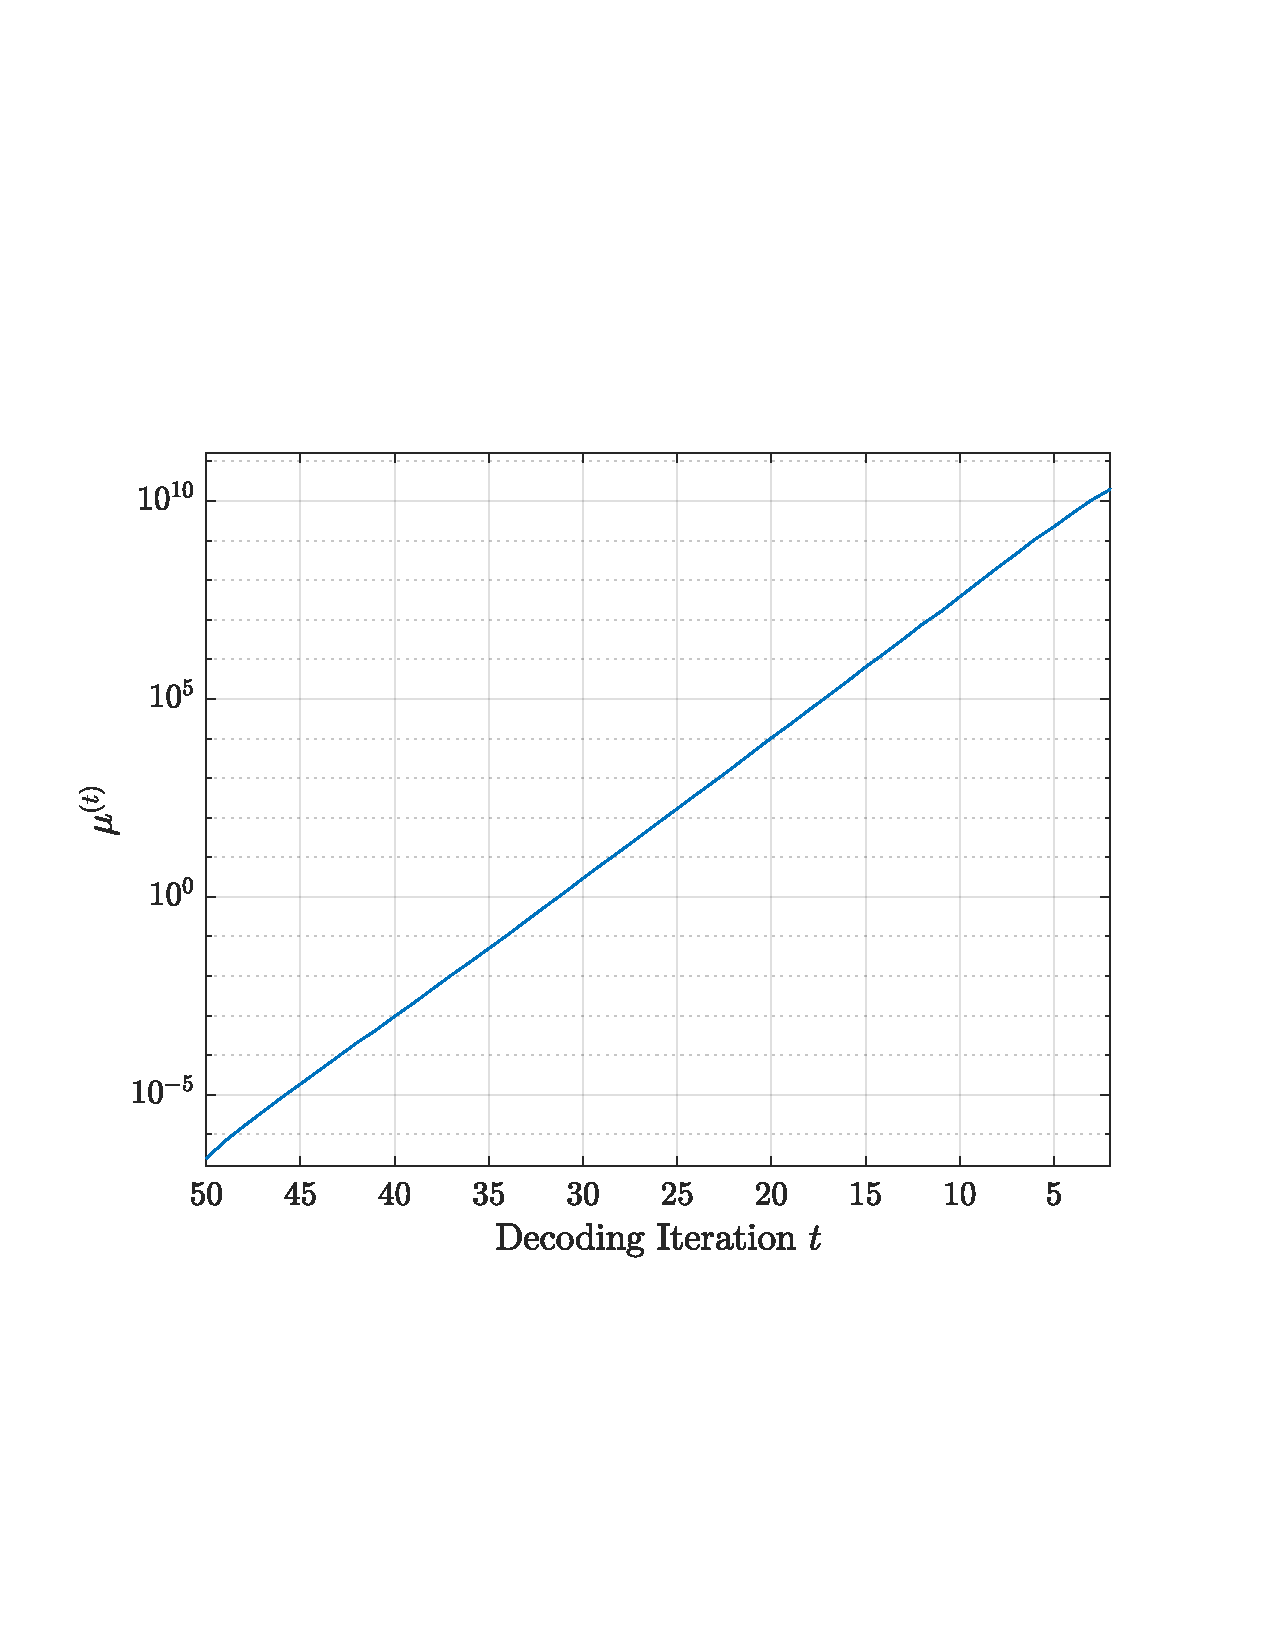
\includegraphics[width=0.50\linewidth]{figures/Gradient_Explosion.pdf}}
    \\
  \subfloat[\label{fig: FER-FNNMS-1}]{%
        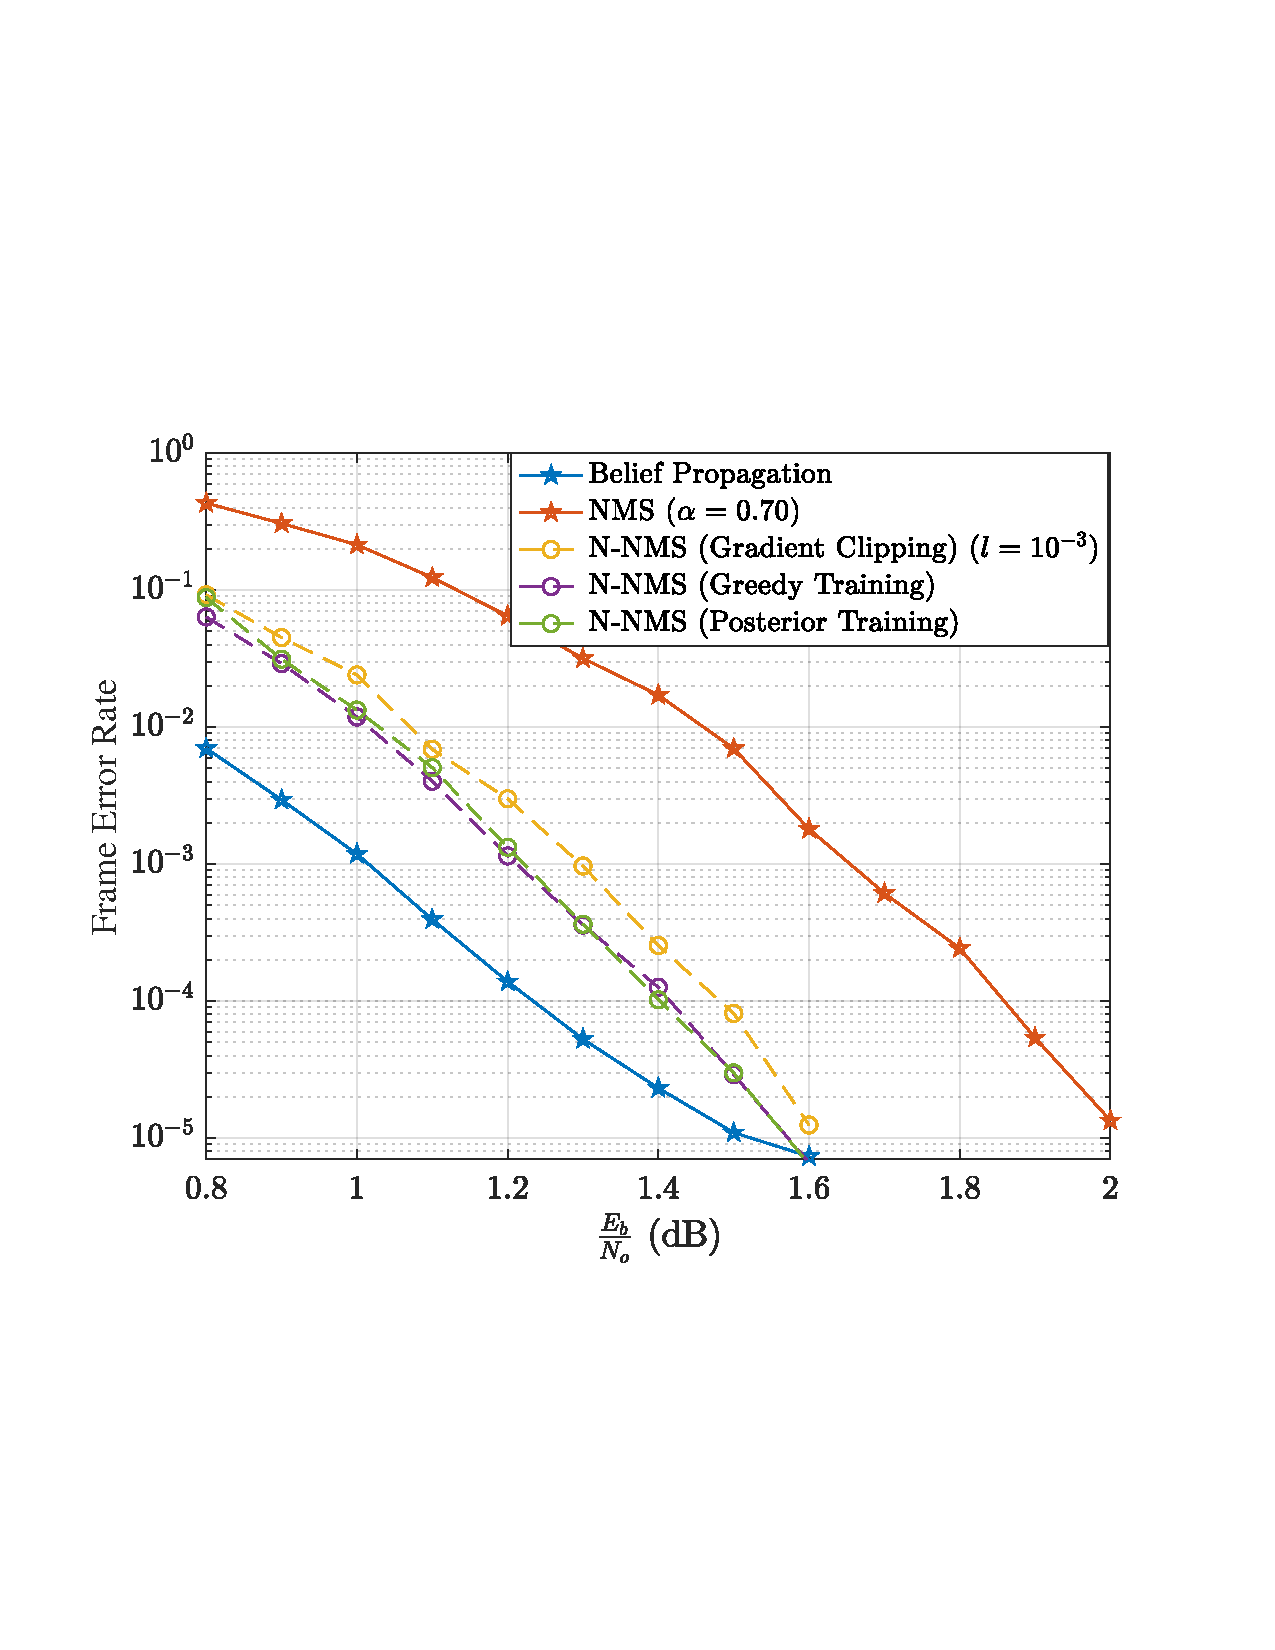
\includegraphics[width=0.50\linewidth]{figures/posterior_training.pdf}}
  \caption{Fig. (a): The average magnitude of gradients of loss $J$ w.r.t. C2V messages in each decoding iteration. The gradients are calculated by feeding the flooding-scheduled (3096,1032) N-NMS decoder with an input sample and performing backward propagation. Fig. (b): FER curves of the flooding-scheduled N-NMS decoders for a (3096,1032) LDPC code.  Gradient clipping, greedy training and posterior jointly training are used to address gradient explosion issue. The maximum decoding iteration is 50. The belief propagation decoder and NMS decoder with factor 0.7 are presented as comparison.}
\end{figure}
Equation \eqref{equ: l_update} implies that in iteration $t$, for all variable nodes that connect check node $c$, only $\texttt{pos1}_{c}^{t}$ and $\texttt{pos2}_{c}^{t}$ receive gradients from $c$. Besides, $|\mathcal{N}(c)|-1$ gradient terms flow to $\texttt{pos1}_{c}^1$. Hence, if check node  $c$ has a large degree, the gradient of $J$ w.r.t. $\texttt{pos1}_{c}^{t}$ can have a large magnitude, and this large-magnitude gradient will be propagated to the neurons in the preceding layer that corresponded to the C2V messages whose check nodes (other than $c$) connect $\texttt{pos1}_{c}^{t}$.  As a result, the large-magnitude gradients are accumulated and propagated as back propagation proceeds, which results in gradient explosion.

Fig. \ref{fig: gradient_explosion} shows the gradient explosion phenomenon when training a flooding-scheduled N-NMS decoder for a (3096,1032) LDPC code. Define $\mu^{(t)}$ as the average magnitude of the gradients of $J$ w.r.t. all C2V messages in iteration $t$. The gradients are calculated by feeding the  N-NMS decoder with some input sample and then performing backward propagation. Fig. \ref{fig: gradient_explosion} plots $\mu^{(t)}$ in each decoding iteration. The maximum check node degree and variable node degree of the code are 19 and 27, respectively. The maximum decoding iteration of the decoder is 50.  It can be seen that the $\mu^{(t)}$ increases exponentially with the decrease of decoding iteration $t$.

\eqref{equ: gradient_beta} indicates that  large magnitude of $\frac{\partial J}{\partial u^{(t)}_{(c,v)}}$ leads to large magnitude of $\frac{\partial J}{\partial \beta^{(t)}_{(c,v)}}$  and hence prevents the neural network from optimizing weights effectively. To the best of our knowledge, this paper is the first one to report the gradient explosion issue for neural LDPC decoder training. However, there have been several techniques that solve the gradient explosion problem:

\begin{enumerate} 
    \item \textit{Gradient Clipping}. Gradient explosion is a common problem in the deep learning field such as recurrent neural network, and one way to solve this problem is gradient clipping \cite{GoodBengCour16}.  There are various methods for gradient clipping \cite{mikolov2012, Pascanu2013-es}. This paper considers to  simply limit the maximum gradient magnitude to be some threshold $l$.
    
    \item \textit{Greedy Training}. Dai \textit{et al} in \cite{dai2021learning} proposed greedy training. Greedy training trains the parameters in $t^{th}$ decoding iteration by fixing the pre-trained parameters in the first $t-1$ iterations. Greedy training solves the gradient explosion problem because the large magnitude gradients won't be accumulated and propagated to the preceding hidden layers, i.e, decoding iterations. 
    However, greedy training requires a time complexity that is proportional to $I_T^2$, because one must have trained the $(t-1)$-iterations decoder in order to train
    a $t$-iterations decoder.
\end{enumerate}

\eqref{equ: update-c} indicates that the gradient of $J$ w.r.t. $u^{(t)}_{c_i\rightarrow v_j}$ comes from two parts: the first part is from the posterior $l^{(t)}_{v_j}$, and the second part is from the V2C messages $l^{(t)}_{v_j\rightarrow c_i'}$, $c_{i'}\in \mathcal{N}(v_j) \setminus \{c_i\}$. Based on the previous analysis, if any $l^{(t)}_{v_j\rightarrow c_i'}$, $c_{i'}\in \mathcal{N}(v_j) \setminus \{c_i\}$ has a large magnitude gradient, the neuron $u^{(t)}_{c_i\rightarrow v_j}$  can also have a large magnitude gradient. This will result in a large magnitude to the gradient of $J$ w.r.t. $\beta^{(t)}_{(c_i,v_j)}$, as indicated by \eqref{equ: gradient_beta}.  In this paper, we propose posterior jointly training which calculates the gradient of $J$ w.r.t. $u^{(t)}_{c_i\rightarrow v_j}$ only using the posterior $l^{(t)}_{v_j}$.  More explicitly, for the flooding-scheduled  N-NMS neural network, $\frac{\partial J}{\partial u^{(t)}_{c_i\rightarrow v_j}}$ is calculated by:
\begin{align}\label{equ: pt_flooding}
         \frac{\partial J}{\partial u^{(t)}_{c_i \rightarrow v_j}} = \frac{\partial J}{\partial l^{(t)}_{v_j}}.
\end{align}
Hence,  the gradient of $J$ w.r.t. $\beta^{(t)}_{(c_i,v_j)}$ is calculated as:
\begin{align}\label{equ: gradient_beta_2}
    \frac{\partial J}{\partial \beta^{(t)}_{c_i \rightarrow v_j}} = \frac{u^{(t)}_{c_i \rightarrow v_j}}{\beta^{(t)}_{c_i\rightarrow v_j}} \frac{\partial J}{\partial u^{(t)}_{c_i\rightarrow v_j}}=\frac{u^{(t)}_{c_i \rightarrow v_j}}{\beta^{(t)}_{c_i\rightarrow v_j}}\frac{\partial J}{\partial l^{(t)}_{v_j}}.
\end{align}

By calculating the gradients of neurons in the $t^{th}$ decoding iteration only using   $l^{(t)}$, i.e., the posteriors in the $t^{th}$ decoding iteration, \eqref{equ: pt_flooding} and \eqref{equ: gradient_beta_2} prevent the large magnitudes that are due to  $\frac{\partial J}{\partial l^{(t)}_{ v_j\rightarrow c_{i'} }}$ from propagating to the preceding hidden layers. This idea resembles the greedy training method. However, the posterior jointly training optimizes parameters of all decoding iterations  jointly, hence it requires a time complexity that is proportional to $I_T$. 
    
For the layer-scheduled N-NMS decoder, the conventional back propagation calculates the gradient of $J$ w.r.t.  $ u^{(t)}_{c_i \rightarrow v_j}$ by:
\begin{align}\label{equ: conv_layer}
    \frac{\partial J}{\partial u^{(t)}_{c_i \rightarrow v_j}} =  \frac{\partial J}{\partial l^{(t)}_{v_j}}+ \sum_{\{i'|c_{i'}\in\mathcal{N}(v_j),i'>i\}}\frac{\partial J}{\partial l^{(t)}_{v_j \rightarrow c_{i'}}}+\sum_{\{i'|c_{i'}\in\mathcal{N}(v_j),i'<i\}}\frac{\partial J}{\partial l^{(t+1)}_{v_j \rightarrow c_{i'}}}.
\end{align}
Posterior jointly training abandons the last term in \eqref{equ: conv_layer} and calculates $\frac{\partial J}{\partial u^{(t)}_{c_i\rightarrow v_j}}$ as follows:
\begin{align}\label{equ: pt_layer}
    \frac{\partial J}{\partial u^{(t)}_{c_i \rightarrow v_j}} =  \frac{\partial J}{\partial l^{(t)}_{v_j}}+ \sum_{\{i'|c_{i'}\in\mathcal{N}(v_j),i'>i\}}\frac{\partial J}{\partial l^{(t)}_{v_j \rightarrow c_{i'}}}.
\end{align}
Fig. \ref{fig: FER-FNNMS-1} shows the frame error rate (FER) of flooding-scheduled N-NMS decoders for a (3096,1032) LDPC code. The maximum decoding iteration time is 50. All three methods are implemented for preventing gradient explosion. Especially, for the gradient clipping,  the threshold for gradient magnitude is $l=10^{-3}$. The performance of BP and NMS with the same decoding schedule and maximum decoding iteration are also given for comparison. The NMS decoder uses multiplicative factor 0.7. The simulation result shows that greedy training and posterior jointly training deliver a better better performance than simple gradient clipping method. Greedy training and posterior jointly training deliver a  similar performance, both of which are 0.4 dB better than conventional  NMS decoder and have a better performance than BP at 1.6 dB. However,  posterior jointly training has a lower time complexity than greedy training.

\section{Node-Degree-Based Weight Sharing}\label{sec: N-2D-NMS}

N-NMS and N-OMS decoder for the long-blocklength LDPC codes are impractical, because the number of parameters of these decoders is proportional to the number of edges in the corresponding Tanner graph. Weight sharing \cite{xie2021weight} solves this problem by assigning one weight to different neurons in the NN. Different weight sharing schemes have been proposed to reduce the number of neural weights in N-NMS and N-OMS decoder. However, simple weight sharing schemes, such as across iterations or edges in \cite{Wang2020-fb,Lian2019-jh}, degrade the decoding performance in different degrees. 
\begin{figure}[hp]
    \centering
  \subfloat[\label{fig: mean-t}]{%
       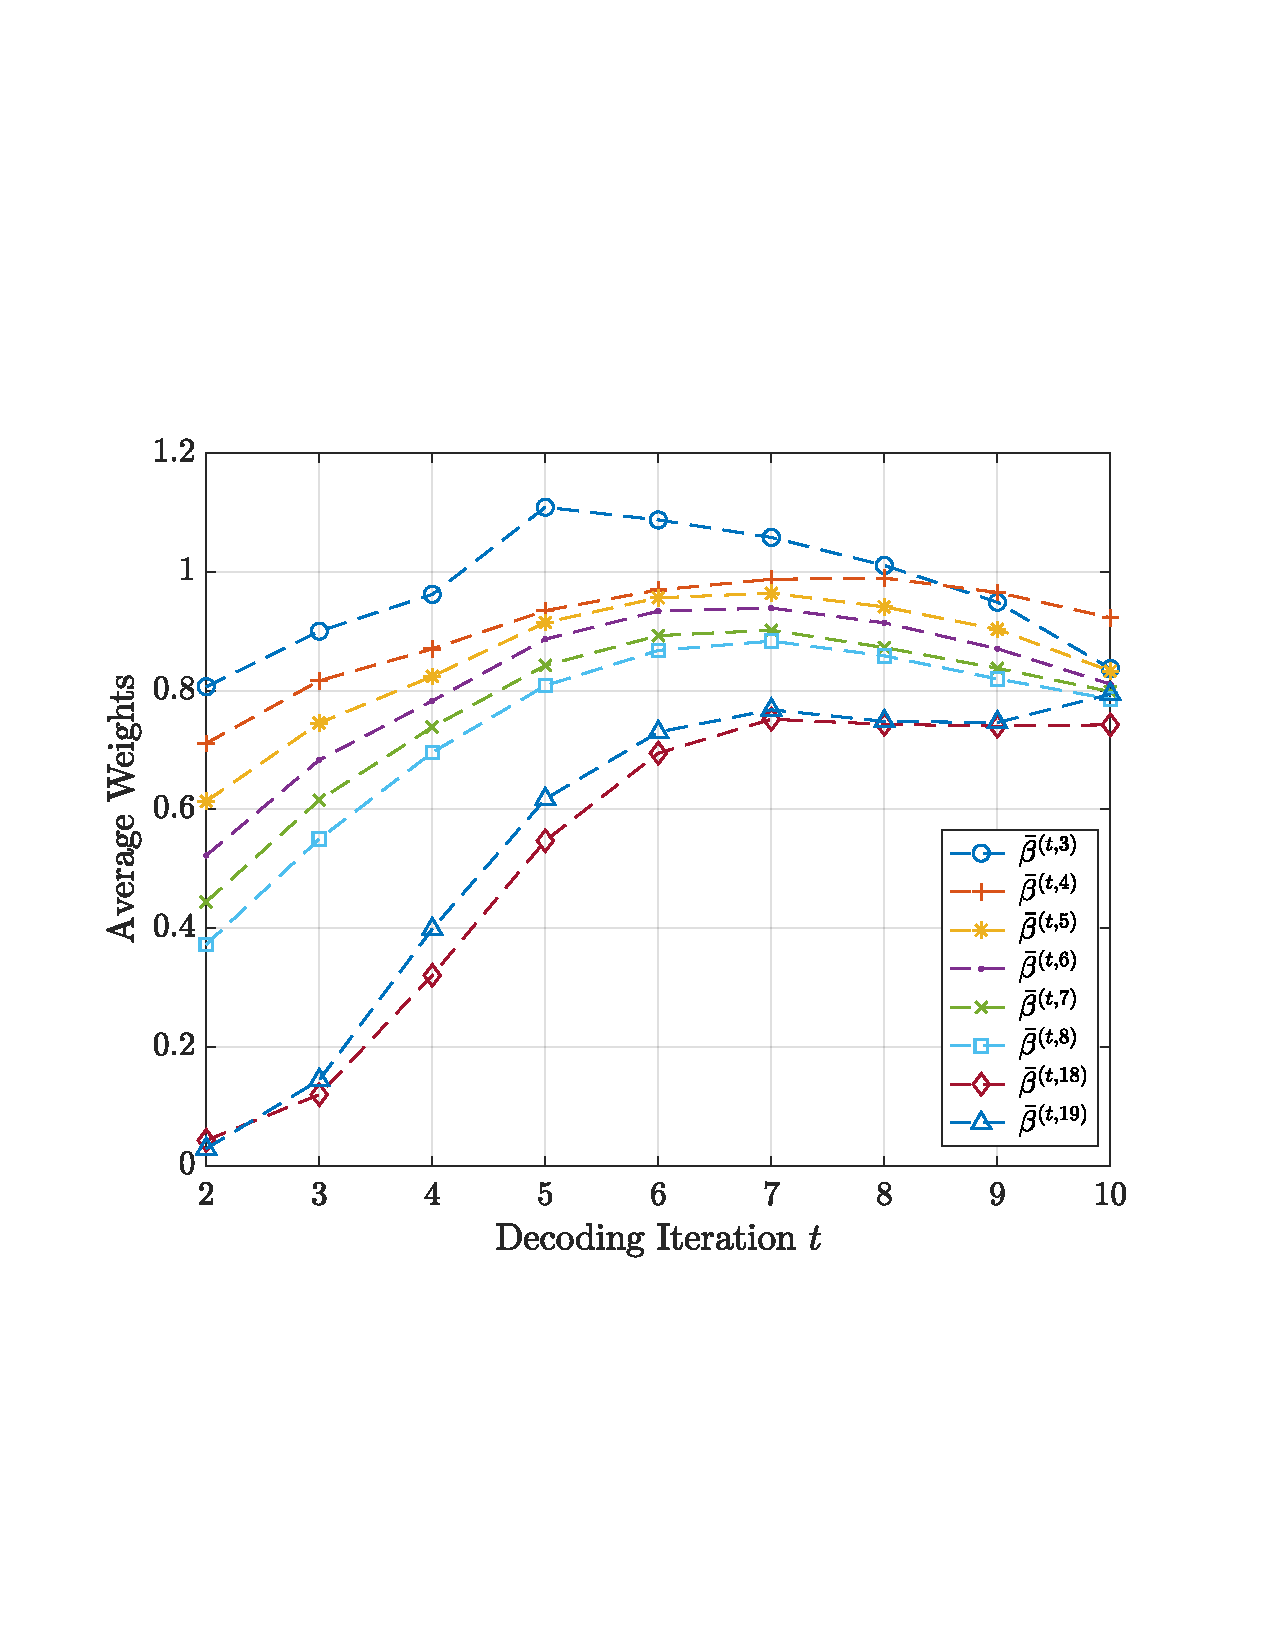
\includegraphics[width=0.50\linewidth]{figures/beta_mean_vs_iteration.pdf}}
    \\
  \subfloat[\label{fig: degree-19-iter4}]{%
        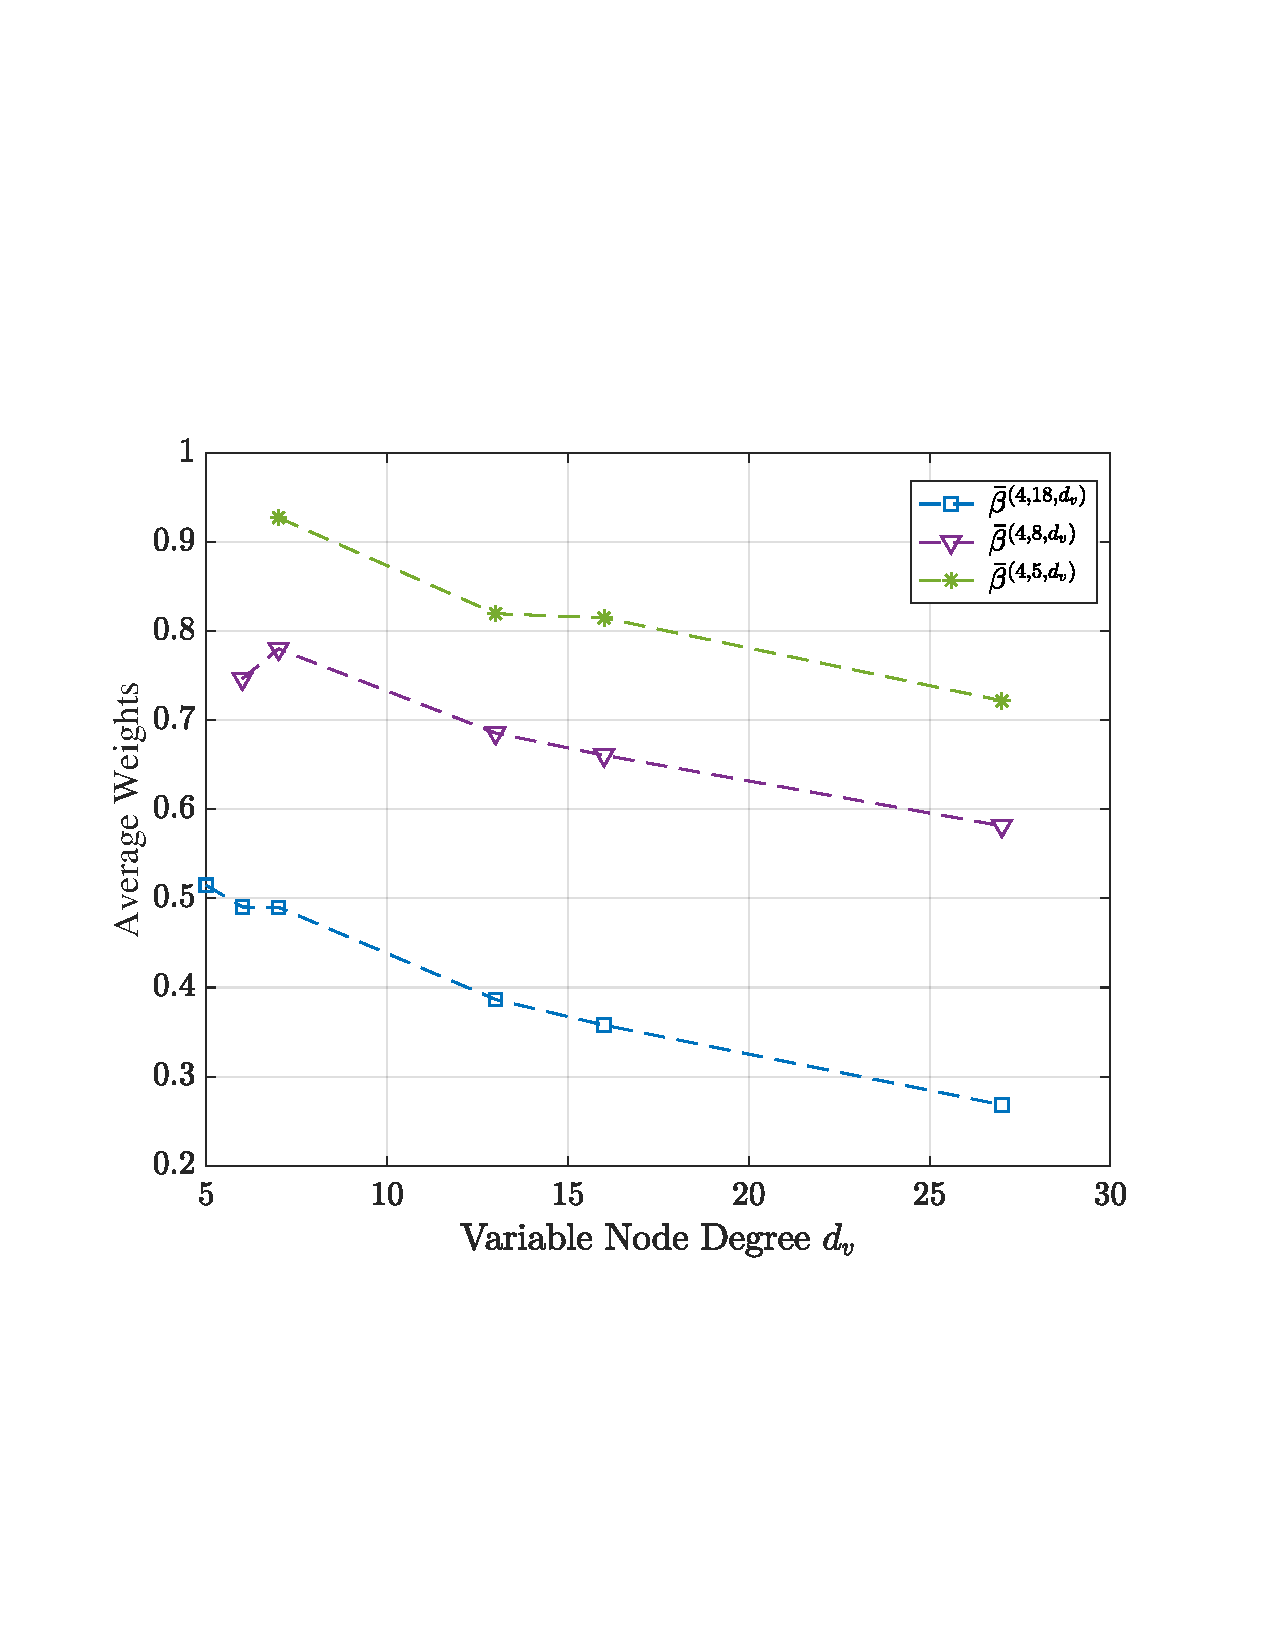
\includegraphics[width=0.50\linewidth]{figures/weight_vn.pdf}}
  \caption{Mean values of messages of a flooding-scheduled N-NMS decoder for a (3096,1032) LDPC code in each iteration show strong correlations to check and variable node degree.}
   \label{fig: weights_evaluation}
\end{figure}
This section proposes node-degree-based weight sharing schemes which assign the same weights to the edges that have same check and/or variable node degree. We call the N-NMS and N-OMS decoder with node-degree-based weight sharing schemes by neural 2-dimensional NMS (N-2D-NMS) and neural 2-dimensional OMS (N-2D-OMS) decoder, respectively,  because they are similar to the 2D-MS decoders in \cite{Juntan_Zhang2005-2dnms,2doms}. Simulation results in Section \ref{sec: Simulation} show that N-2D-NMS decoder can deliver the same decoding performance with N-NMS decoder.

\subsection{Motivation}
In this subsection, we investigate the relationship between the neural weights of a flooding-scheduled N-NMS decoder and node degrees. 
The N-NMS decoder is trained for a  (3096, 1032) LDPC code, the same one used in Section  \ref{Sec: gradient_explosion}. The maximum decoding iteration is 10.

Define the set of neural weights of N-NMS decoder that are associated to check node degree $d_c$ in the $t^{th}$ decoding iteration by $\mathcal{B}^{(t,d_c)}$, and $\mathcal{B}^{(t,d_c)}=\{\beta^{(t)}_{(c_i,v_j)}|\text{deg}(c_i) = d_c\}$. Let $\bar{\beta}^{(t,d_c)}$ be the mean value of $\mathcal{B}^{(t,d_c)}$. Fig.\ref{fig: mean-t} shows $\bar{\beta}^{(t,d_c)}$ versus decoding iteration $t$ with all possible check node degrees. The simulation result shows a clear relationship between check node degree and $\bar{\beta}^{(t,d_c)}$, i.e. a larger check node degree corresponds to a smaller $\bar{\beta}^{(t,d_c)}$. This difference is significant in the first few iterations.
Additionally, $\bar{\beta}^{(t,d_c)}$ changes drastically in first few iterations for all check node degrees. 

In order to explore the relationship between the weights and variable node degrees given a check node degree $d_c$ and decoding iteration index $t$, we further define $ \mathcal{B}^{(t,d_c,d_v)}=\{\beta^{(t)}_{(c_i,v_j)}\allowbreak| \text{deg}(c_i)=d_c,\text{deg}(v_i)=d_v\}$. We denote  the average value of $\mathcal{B}^{(t,d_c,d_v)}$ by $\bar{\beta}^{(t,d_c,d_v)}$. Fig.\ref{fig: degree-19-iter4} gives the average weights corresponding to various check and variable node degrees at iteration $4$. Statistical results show that, given a specific iteration $t$ and check node degree $d_c$, a larger $d_v$ indicates a smaller $\bar{\beta}^{(t,d_c,d_v)}$. 

In conclusion, the weights of N-NMS decoder are correlated with check node degree, variable node degree, and decoding iteration index. Thus, node degrees should affect the weighting of messages on their incident edges when decoding LDPC codes. This observation motivates us to propose a family of N-2D-MS decoders in this paper. 
\begin{center}
    % Please add the following required packages to your document preamble:
% \usepackage{multirow}

\begin{table}[t]
    \centering
    \small
    \caption{Various Node-Degree-Based Weight Sharing Schemes and Required Number of Parameters per Iteration for Two Example Codes}
    \begin{tabular}{|c|c|c|c|c|}
    \hline
    \multirow{2}{*}{Type} & \multirow{2}{*}{$\beta^{(t)}_{*}$}                                    & \multirow{2}{*}{$\alpha^{(t)}_{*}$}                & \multicolumn{2}{c|}{\begin{tabular}[c]{@{}c@{}}The Number of Required\\  Parameters per Iteration\end{tabular}}                        \\ \cline{4-5} 
                          &                                                                       &                                                    & (16200,7200) DVBS-2 code & (3096,1032)  PBRL code \\ \hline
    \multicolumn{5}{|c|}{No Weight Sharing\cite{Nachmani2016-bs}}                                                                                                                                                                                                                                                     \\ \hline
    $0$            & $\beta^{(t)}_{(c_i,v_j)}$                                             & 1                                                  & $4.8*10^5$                                                          & $1.60*10^4$                                                      \\ \hline
    \multicolumn{5}{|c|}{Weight Sharing Based on Node Degree}                                                                                                                                                                                                                                   \\ \hline
    1                     & $\beta^{(t)}_{(\text{deg}{(c_i)},\text{deg}{(v_j)})}$                                 & 1                                                  & 13                                                                  & 41                                                               \\ \hline
    2                     & $\beta^{(t)}_{(\text{deg}{(c_i)})}$                                          & $\alpha^{(t)}_{(\text{deg}{(v_j)})}$                      & 8                                                                   & 15                                                               \\ \hline
    3                     & $\beta^{(t)}_{(\text{deg}{(c_i)})}$                                          & 1                                                  & 4                                                                   & 8                                                                \\ \hline
    4                     & 1                                                                  & $\alpha^{(t)}_{(\text{deg}{(v_j)})}$                      & 4                                                                   & 7                                                                \\ \hline
    \multicolumn{5}{|c|}{Weight Sharing Based on Protomatrix}                                                                                                                                                                                                                                   \\ \hline
    5\cite{dai2021learning}          & $\beta^{(t)}_{\left( \floor{\frac{i}{f}},\floor{\frac{j}{f}}\right)}$ & 1                                                  & $-$                                                                 & 101                                                              \\ \hline
    6                     & $\beta^{(t)}_{\left( \floor{\frac{i}{f}}\right)}$                     & 1                                                  & $-$                                                                 & 17                                                               \\ \hline
    7                     & 1                                                                       & $\alpha^{(t)}_{\left( \floor{\frac{j}{f}}\right)}$ & $-$                                                                 & 25                                                               \\ \hline
    \multicolumn{5}{|c|}{Weight sharing based on Iteration  \cite {Lian2019-jh,Abotabl2019-wt}}                                                                                                                                                                                                          \\ \hline
    8                     & $\beta^{(t)}$                                                         & 1                                                  & 1                                                                   & 1                                                                \\ \hline
    \end{tabular}\label{tab:weight_sharing}
    \end{table}
\end{center}
\subsection{Neural 2D Normalized MinSum Decoders}
Based on the previous discussion, it is intuitive to consider assigning the same weights to messages with same check node degree and/or variable node degree. 
In this subsection, we propose a family node-degree-based weight sharing schemes.
These weight sharing schemes can be used on the  N-NMS decoder, which gives N-2D-NMS decoder. 

In the $t^{th}$ iteration, a flooding-scheduled N-2D-NMS decoder update $u^{(t)}_{c_i\rightarrow v_j}$ as follows:
\begingroup
\allowbreak
\begin{align}
     u^{(t)}_{c_i\rightarrow v_j} &= \beta^{(t)}_{*} \times  \prod_{v_{j'}\in \mathcal{N}(c_i)/\{v_j\}} \text{sgn}\left(l^{(t-1)}_{v_{j'}\rightarrow c_{i}}\right)  \times  \min_{v_{j'}\in \mathcal{N}(c_i)/\{v_j\}} \left|l^{(t-1)}_{v_{j'}\rightarrow c_{i}}\right|.\\
      l^{(t)}_{v_j\rightarrow c_i} &=  l^{ch}_{v_i} + \alpha^{(t)}_{*}  \sum_{c_{i'}\in \mathcal{N}(v_j)/\{c_i\}} u^{(t)}_{c_{i'}\rightarrow v_j},\\
    l^{(t)}_{v_j} &=  l^{ch}_{v_i} + \alpha^{(t)}_{*}  \sum_{c_{i'}\in \mathcal{N}(v_j)} u^{(t)}_{c_{i'}\rightarrow v_j}.
\end{align}
\endgroup




$\beta^{(t)}_{*}$ and $\alpha^{(t)}_{*}$ are the learnable weights. The subscript * is replaced in Table \ref{tab:weight_sharing} with the information needed to identify the specific weight depending on the weight sharing methodology. 
Table \ref{tab:weight_sharing} lists different weight sharing types, each identified in the first column by a type number. As a special case, we denote type 0 by assigning distinct weights to each edge, i.e., N-NMS decoder. Columns 2 and 3 describe how each type assigns $\beta^{(t)}_{*}$ and $\alpha^{(t)}_{*}$, respectively. In this paper, we refer to a decoder that uses a type-$x$ weight sharing scheme as a type-$x$ decoder. 

Types 1-4 assign the same weights based on node degree. In particular, Type 1 assigns the same weight to the edges that have same check node \emph{and} variable node degree. Type 2 considers the check node degree and variable node degree separately. As a simplification, type 3 and type 4 only consider check node degree and variable node degree, respectively.

Dai. \emph{et. al} in \cite{dai2021learning} studied weight sharing based on the edge type of multi-edge-type (MET)-LDPC codes, or protograph-based codes. We also consider this metric for types 5, 6, and 7. Type 5  assigns the same weight to the edges with the same edge type, i.e., the edges that belong to the same position in protomatrix. In Table. \ref{tab:weight_sharing}, $f$ is the lifting factor.  Types 6 and 7 assign parameters based only on the horizontal (protomatrix row) and vertical layers (protomatrix column), respectively.
Finally, type 8 assigns a single weight to all edges in each decoding iteration, as in \cite{Lian2019-jh,Abotabl2019-wt}. 

A (3096,1032) LDPC code and the (16200,7200) DVBS-2\cite{noauthor_2019-nv} standard LDPC code are considered in this section, and the number of parameters per iteration required for various weight sharing schemes of these two codes are listed in column 4 and 5 in Table. \ref{tab:weight_sharing}, respectively. It is shown that the number of parameters required by the node-degree-based weight sharing is less than that required by the protomatrix-based weight sharing.

\subsection{Neural 2D Offset MinSum Decoder}
The node-degree-based weight sharing schemes can be applied to N-OMS decoder in a similar way and lead to neural 2D OMS (N-2D-OMS) decoder. Specifically, a flooding N-2D-OMS decoder updates  $u^{(t)}_{c_i\rightarrow v_j}$ by: 
\begin{align}
     u^{(t)}_{c_i\rightarrow v_j} &= \prod_{v_{j'}\in \mathcal{N}(c_i)/\{v_j\}} \text{sgn}\left(l^{(t-1)}_{v_{j'}\rightarrow c_{i}}\right)  \times   \text{ReLu} \left(\min_{v_{j'}\in \mathcal{N}(c_i)/\{v_j\}} \left|(l^{(t-1)}_{v_{j'}\rightarrow c_{i}})\right|-\beta^{(t)}_*-\alpha ^{(t)}_*\right).
\end{align}
${\mathrm{ReLu}}(x)=\max(0,x)$. The $l_{v_j\rightarrow c_i}^{(t)}$ and $l_{v_j}^{(t)}$ are updated using \eqref{equ: v2c_update} and \eqref{equ: pos_update}. For the N-2D-OMS decoders, the constant value 1 in Table \ref{tab:weight_sharing} should be replaced by 0. 

\subsection{Hybrid Neural Decoder}
To further reduce the number of parameters, we consider a hybrid training structure that utilizes a neural network combining a feed forward module with a recurrent module. The corresponding decoder uses distinct neural weights for each of the first $I'$ decoding iterations and uses the same weights 
for the remaining  $I_T-I'$ iterations.
The motivation for the hybrid decoder is from the observation that the neural weights of N-NMS decoder change drastically in the first few iterations, but negligibly during the last few iterations, as illustrated in Fig. \ref{fig: weights_evaluation}. Therefore, using the same parameters for the last few iterations doesn't cause a large performance degradation. 

\section{Weighted RCQ Decoder}\label{sec: W-RCQ}
This section combines the N-2D-NMS or N-2D-OMS decoder with RCQ decoding paradigm and proposes a weighted RCQ (W-RCQ) decoder. Unlike the RCQ decoder, whose quantizers and de-quantizers are updated in each iteration (and each layer, if layer-scheduled decoding is considered), W-RCQ decoder only uses a small number of quantizers and dequantizers during the decoding process. However, the C2V messages of W-RCQ decoder will be weighted by dynamic node-degree-based parameters that that are trained by a QNN.
\begin{figure}[t]
	\centering
	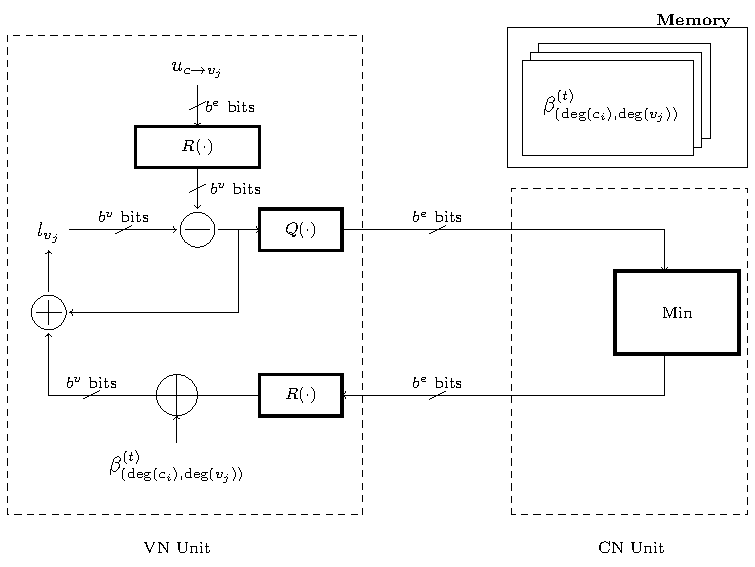
\includegraphics[width=20pc]{figures/neural_rcq.pdf}
	\caption{Layer-scheduled Neural Offset RCQ Decoder Structure}
    \label{fig: layered_neural_RCQ_str}
\end{figure}
\subsection{Structure}
Fig. \ref{fig: layered_neural_RCQ_str} gives the decoding paradigm of a layer-scheduled weighted OMS-RCQ decoder (W-OMS-RCQ).
The offset parameters in Fig. \ref{fig: layered_neural_RCQ_str}, $\beta^{(t)}_{({\mathrm{deg}}(c_i),{\mathrm{deg}}(v_j))}$, use type-1 weight sharing scheme in the Table \ref{tab:weight_sharing}. $b^c$ denotes the bit width of C2V message,  and $b^v$ denotes the bitwidth for V2C message and variable node posterior. 
$l_{v_j}$ is the posterior of variable node $v_j$. 
In the $t^{th}$ iteration, a layer-scheduled W-OMS-RCQ decoder calculates the messages $u^{(t)}_{c_i\rightarrow v_{j'}}$ and updates the posteriors $l_{v_{j'}}$ as follows: 
\begingroup
\allowdisplaybreaks
\begin{align}
     &{\tilde{l}}_{v_{j'} \rightarrow c_{i}} \leftarrow  l_{v_{j'}}-{\mathrm{Relu}}\left( R\left(u^{(t-1)}_{c_i\rightarrow v_{j'}}\right)-\beta^{(t-1)}_{({\mathrm{deg}}(c_i),{\mathrm{deg}}(v_{j'}))}\right),~~\forall j'\in\mathcal{N}(c_i),\\
     &{l}^{(t)}_{v_{j'}\rightarrow c_i} = Q\left(\tilde{l}^{(t)}_{v_{j'}\rightarrow c_i}\right),~~\forall j'\in\mathcal{N}(c_i),\\
    &u^{(t)}_{c_i\rightarrow v_{j'}} =
    \left(\prod_{\tilde{j}\in\mathcal{N}(c_i)\setminus\{{j'}\}}{\mathrm{sgn}}\left(l_{v_{\tilde{j}}\rightarrow c_i}\right)\right)\times \min_{\tilde{j}\in\mathcal{N}(c_i)/\{{j'}\}}\left|l_{v_{\tilde{j}}\rightarrow c_i}\right|,~~\forall j'\in\mathcal{N}(c_i), \\
    &l_{v_{j'}} \leftarrow  {\tilde{l}}_{v_{j'}\rightarrow c_i}+{\mathrm{Relu}}\left( R\left(u^{(t)}_{c_i\rightarrow v_{j'}}\right)-\beta^{(t)}_{(\text{deg}(c_i),\text{deg}(v_{j'}))}\right), ~~\forall j'\in\mathcal{N}(c_i).
\end{align}
\endgroup
The differences between W-RCQ decoder and RCQ decoder are:
\begin{itemize}
    \item \textit{Reconstruction and Quantization}. The reconstruction and quantization functions in a layer-scheduled RCQ decoder are dynamic, which means that the decoder updates $R(\cdot)$ and $Q(\cdot)$ in each decoding layer and iteration. Storing the quantizers and dequantizers of all layers and iteration in the local variable node units (VNUs) will cost large amount of LUTs, hence a central control unit is considered for storing and distributing the parameters to each VNU\cite{terrill2021fpga}. 
    On the other hand, the neural RCQ decoder only uses very few number of $R(\cdot)$ and $Q(\cdot)$ across all decoding iterations, for example, three or less. Besides, as will be seen in the next subsection, we require that the thresholds of quantizers and mapping values of dequantizers have the same values. Each $R(\cdot)$ and $Q(\cdot)$ are used for several iterations. Hence,  $R(\cdot)$ and $Q(\cdot)$ are possible to be stored locally in VNUs.
    \item \textit{Message adjustment}. W-RCQ decoder weights the reconstructed C2V messages with additive or multiplicative parameters, which result in W-OMS-RCQ and W-NMS-RCQ, respectively. As shown in Fig. \ref{fig: layered_RCQ_str}, a central control unit is used for storing and distributing the weights to VNUs.
\end{itemize}

\subsection{Non-Uniform Quantizer}
An important design choice for a W-RCQ decoder is  the selection of quantization and reconstruction (dequantization) function. The authors in \cite{wang2022TCOMRCQ} use discrete density evolution to design dynamic quantizers and dequantizers. In \cite{Zhang2014-ib}, Zhang \emph{et. al.} point that  the message magnitude of iterative LDPC decoders can exhibit exponential behavior as a function of the number of decoding iterations, and the decoding performance of a quantized decoder can be improved by allowing exponential growth magnitude.  For example,  the authors in \cite{Zhang2014-ib} propose a ($q$+1)-bit quasi-uniform quantizer that uses one extra bit to efficiently
increase the dynamic range of messages.
For the W-RCQ decoder, this paper considers the quantizer and dequantizer that can be parameterized by a power function. 

Let $Q(x)$ be a symmetric $b^c$-bit quantizer that features sign information and a magnitude quantizer $Q^*(|x|)$. The magnitude quantizer selects one of $2^{b^\text{c}-1}$ possible indices using the threshold values $\{\tau_0,\tau_1,\ldots,\tau_{\text{max}}\}$, where  $\tau_j=C\left(\frac{j}{2^{b^c-1}}\right)^{\gamma}$ for $j\in\{0,\ldots,2^{b^{c}-1}-1\}$ and $\tau_{\text{max}}$ is $\tau_{j_{\text{max}}}$ for $j_{\text{max}} = 2^{b^\text{c}-1}-1$.
Given an input $x$, which can be decomposed into sign part ${{\mathrm{sgn}}(x)}$ and magnitude part $|x|$, $Q^*(|x|)\in \mathbb{F}_2^{b^{\mathrm{c}}-1}$ is defined by:
\begin{align}
    {Q}^*(|x|)=\left\{\begin{matrix}
  j, &    \tau_j\leq|x|<\tau_{j+1}\\
  2^{b_c-1}-1, & |x|\geq \tau_{\mathrm{max}} 
 \end{matrix}\right.,
 \label{equ: 10}
 \end{align}
 where $0\leq j\le j_{\text{max}}$. Let $s(x)$ be the sign bit of $x$, which is defined as $s(x)=\mathbbm{1}(x<0)$, $Q(x)$ is defined as
$Q(x)=[s(x)~Q^*(|x|)]$. The set of thresholds of $Q^*(|x|)$ has a power-function form and is controlled by two parameters. The parameter $C$ confines the maximum magnitudes the quantizer can take, and $\gamma$ manipulates the non-uniformity of the quantizer. 
Specifically, if $\gamma=1$,  $Q(x)$ becomes a uniform quantizer.

Let $d\in\mathbb{F}_2^{b^c}$ be a $b^c$-bit message. $d$ can be represented as $[d^{\text{MSB}}\ \tilde{d}]$, where $d^{\text{MSB}}\in\{0,1\}$ indicates sign and $\Tilde{d}\in\mathbb{F}_2^{b^\text{c}-1}$ corresponds to magnitude. The magnitude reconstruction function ${R}^*(\tilde{d}) = C\left(\frac{\tilde{d}}{2^{b_c}-1}\right)^{\gamma}$,
and $R(d)=(-2d^{\mathrm{MSB}}+1)R^*(\tilde{d})$. Note that both the magnitude quantization function and magnitude reconstruction function use  $\{\tau_1,\ldots,\tau_{\text{max}}\}$ as their parameters. 

The number of  required quantizer/dequantizer pairs for W-RCQ decoder can vary under different circumstances. If the code has a small variable node degree and the bit width of the quantizer is not too low (for example, 4 bits), one quantizer/dequantizer pair is sufficient through all decoding iterations. However, if the variable node degree of the LDPC code is high, or the bit width of quantizer is very small, using one quantizer/dequantizer pair is not able to accommodate the range of messages in the decoding process while providing a fine enough resolution, and is likely to degrade decoding performance. Therefore, we consider to use multiple quantizer/dequantizer pairs, and each pair is used for several iterations.

\subsection{Training Quantized Neural Network}
In this paper, we use the multi-loss cross entropy as the loss function and use posterior jointly training to train the QNN that is associated to the W-RCQ decoder. 
The parameters of the quantizers and dequantizers are fixed before training the neural network.
One problem of QNN is that quantization functions results in zeros derivatives almost everywhere.
In this work, we use a straight through estimator (STE)\cite{Bengio2013-kn, Xiao2020-sb} in the backward propagation. 

\subsection{Fixed-Point W-RCQ decoder}
This paper uses the pair ($b^c$,$b^v$) to denote the bitwidth for fixed-point decoders, where $b^c$ is the bitwidth of C2V messages and $b^v$ is the bitwith of V2C messages and the posteriors of variable nodes. For the W-RCQ decoders,  the learnable parameters are first trained under a floating point message representation and then quantized to $b^v$ bits. 

\begin{table}[t]
    \centering
    \caption{LDPC Codes used for Simulation}
    \begin{tabular}{|c|c|l|}
    \hline
    Code & Rate & \multicolumn{1}{c|}{Edge distribution} \\ \hline
    \multicolumn{1}{|c|}{\begin{tabular}[c]{@{}c@{}}(16200,7200) \\DVBS-2 LDPC code\\\cite{noauthor_2019-nv}\end{tabular}} & $\frac{4}{9}$ & \begin{tabular}[c]{@{}l@{}}$\lambda(x)=2.06*10^{-5}+0.3703x+$\\$0.3333x^2+0.2963x^7$\\ $\rho(x)=0.1186x^3+0.3332x^4+$\\$0.4445x^5+0.1037x^6$\end{tabular} \\ \hline
    \begin{tabular}[c]{@{}c@{}}(9472,8192)\\ QC-LDPC code\\ \cite{wang2022TCOMRCQ}\end{tabular} & $\frac{8}{9}$ & \begin{tabular}[c]{@{}l@{}}$\lambda(x)=x^3$\\ $\rho(x)=0.3919x^{28}+0.6081x^{29}$\end{tabular} \\ \hline
    \begin{tabular}[c]{@{}c@{}}$k=1032$ \\ PBRL LDPC code\\\cite{cls_tool}\end{tabular} & $\frac{8}{9}, \frac{8}{10},\dots,\frac{8}{24}$ & \begin{tabular}[c]{@{}l@{}}$\lambda(x)=0.1190+0.7940x^4+0.0952x^5+$\\ $0.0556x^6+0.3095x^{12}+0.1270x^{16}+0.2143x^{26}$\\ $\rho(x)=0.0238x^2+0.0635x^3+0.0794x^4+$\\ $0.1905x^5+0.2222x^6+0.1270x^7+0.1429x^{17}+$\\ $0.1508x^{18}$\end{tabular} \\ \hline
    \end{tabular}\label{tab: code_info}
    \end{table}

\section{Simulation Result and Discussion}\label{sec: Simulation}
This section evaluates the performance of the N-2D-NMS decoder and the W-RCQ decoder for LDPC codes with different block lengths and code rates. The LDPC codes used in this section are listed in Table \ref{tab: code_info}. All the encoded bits are modulated by binary phase-shift keying (BPSK) and transmitted through a Additive White Gaussian Noise (AWGN) channel. 


\begin{figure}[hp]
    \centering
    \subfloat[\label{fig: dvbs2-fer}]{%
        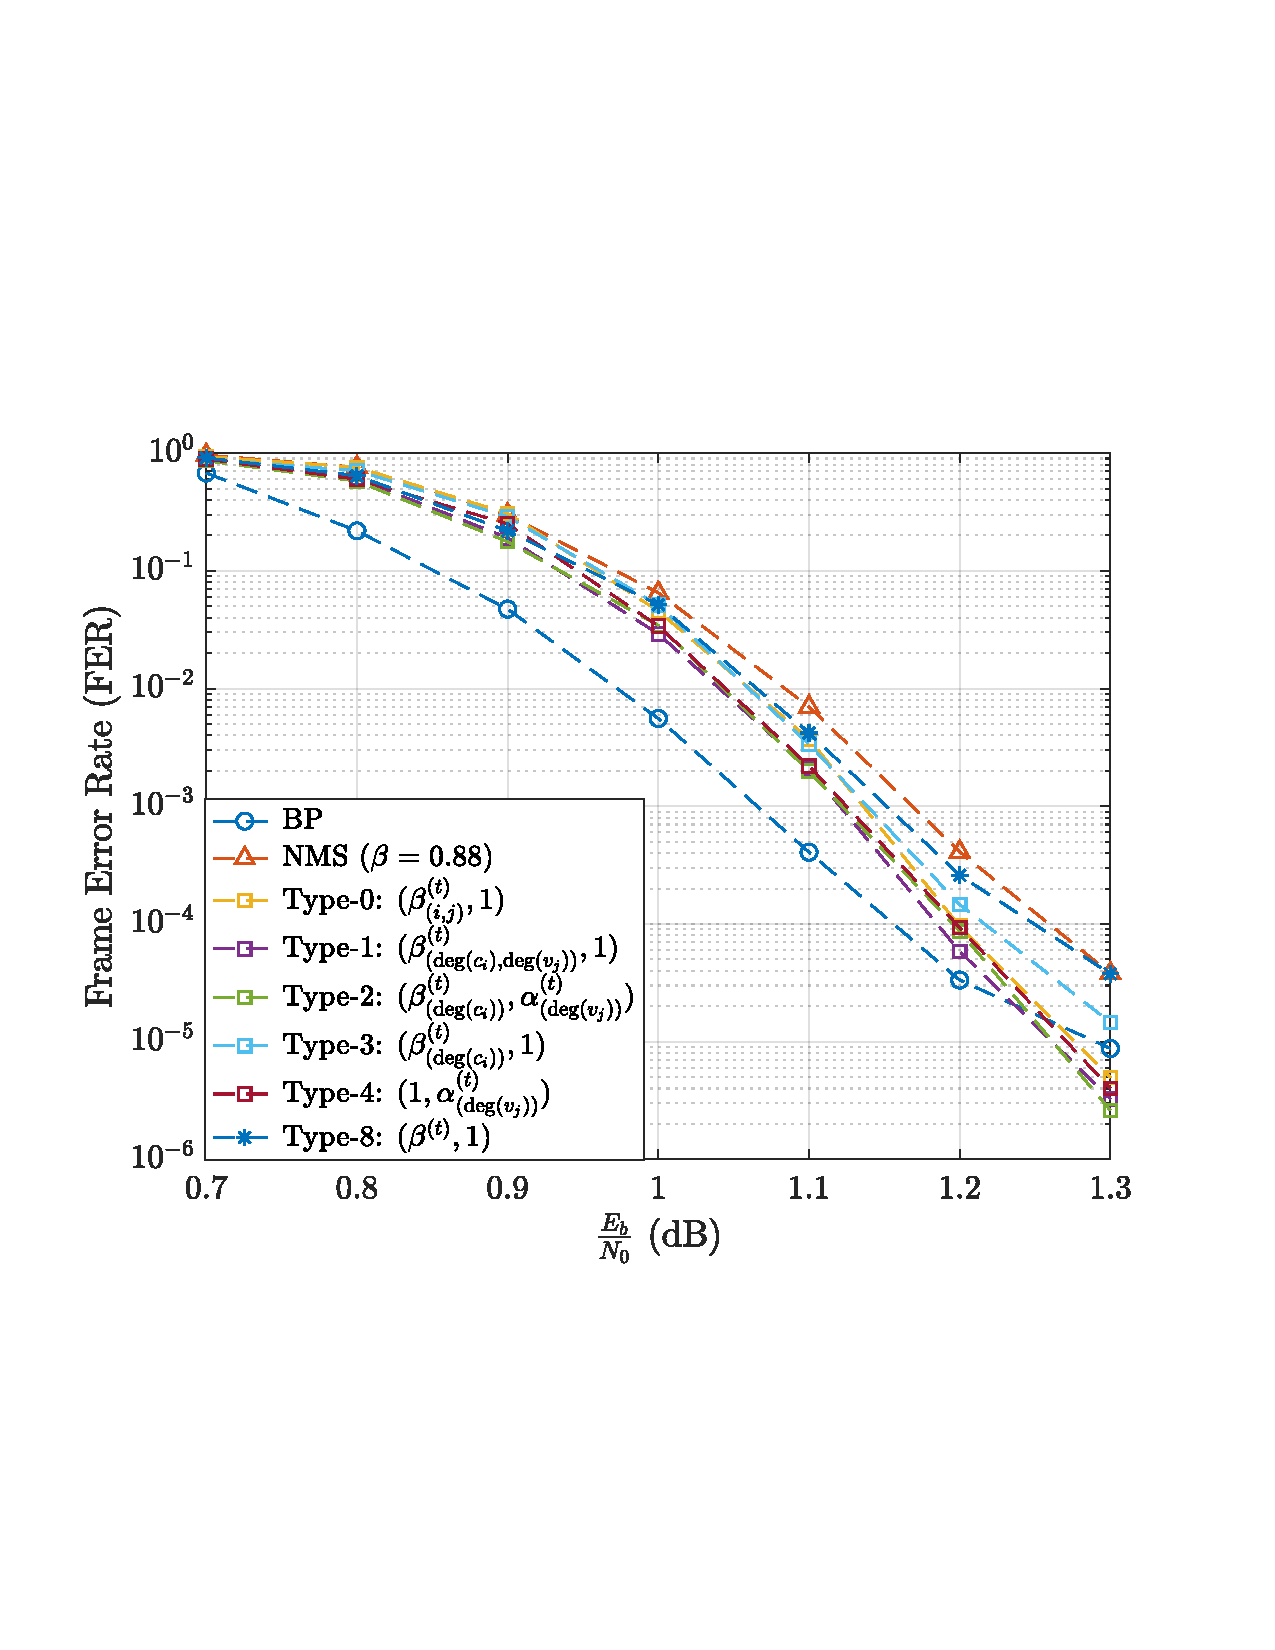
\includegraphics[width=0.50\linewidth]{figures/fig5_a.pdf}}
    \\
    \subfloat[\label{fig: dvbs2-fer2}]{%
        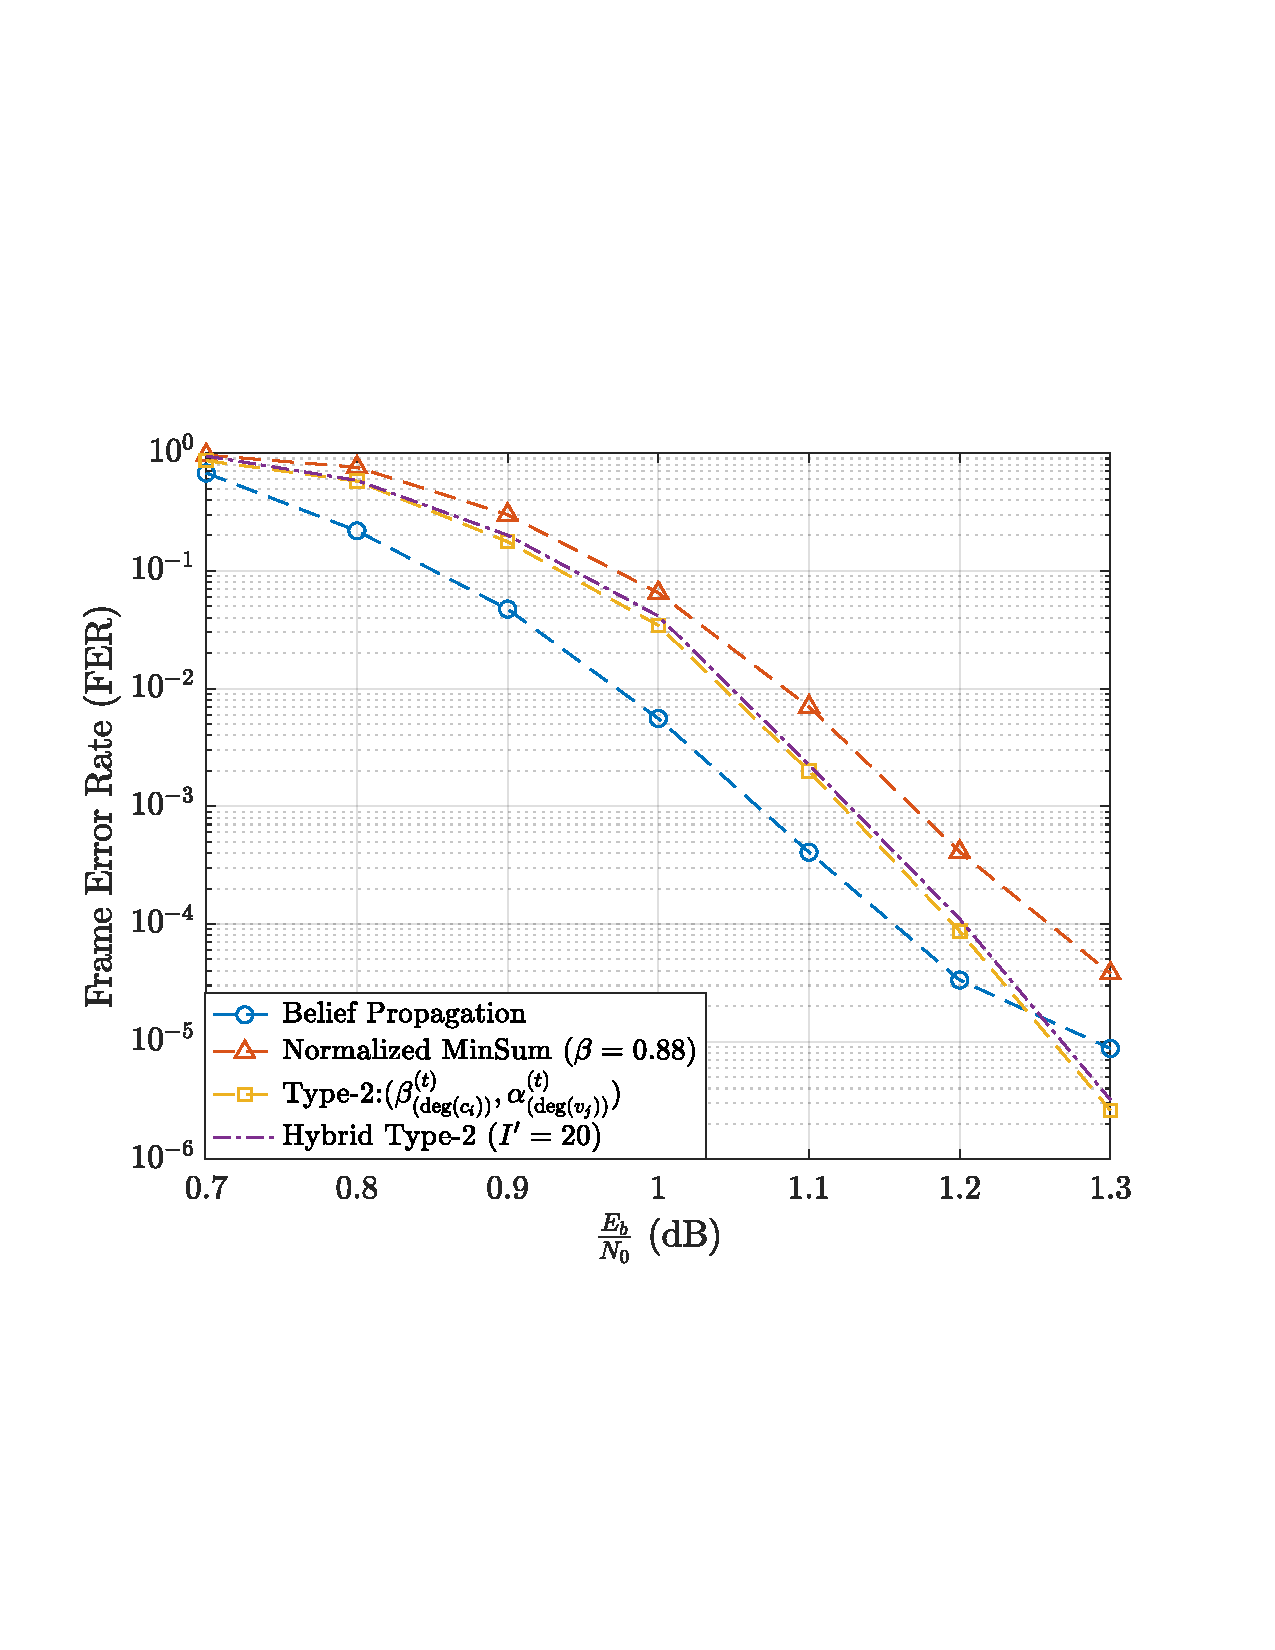
\includegraphics[width=0.50\linewidth]{figures/fig5_b.pdf}}
    \caption{ Fig. (a): The FER performance of
        the N-2D-NMS decoders with various weight sharing types for the (16200,7200) DVBS-2 LDPC code.
        Fig. (b): The FER performance of the hybrid type-2 N-2D-NMS decoder that uses distinct weights in the first 20 iterations and same weights in the remaining 30 iterations. Simulation result shows that the hybrid type-2 N-2D-NMS decoder has comparable decoding performance with the type-2 N-2D-NMS decoder that assigns distinct weights in each iteration.  }
\end{figure}

\begin{figure}[hp] 
    \centering
 \subfloat[\label{fig: beta_iter}]{%
       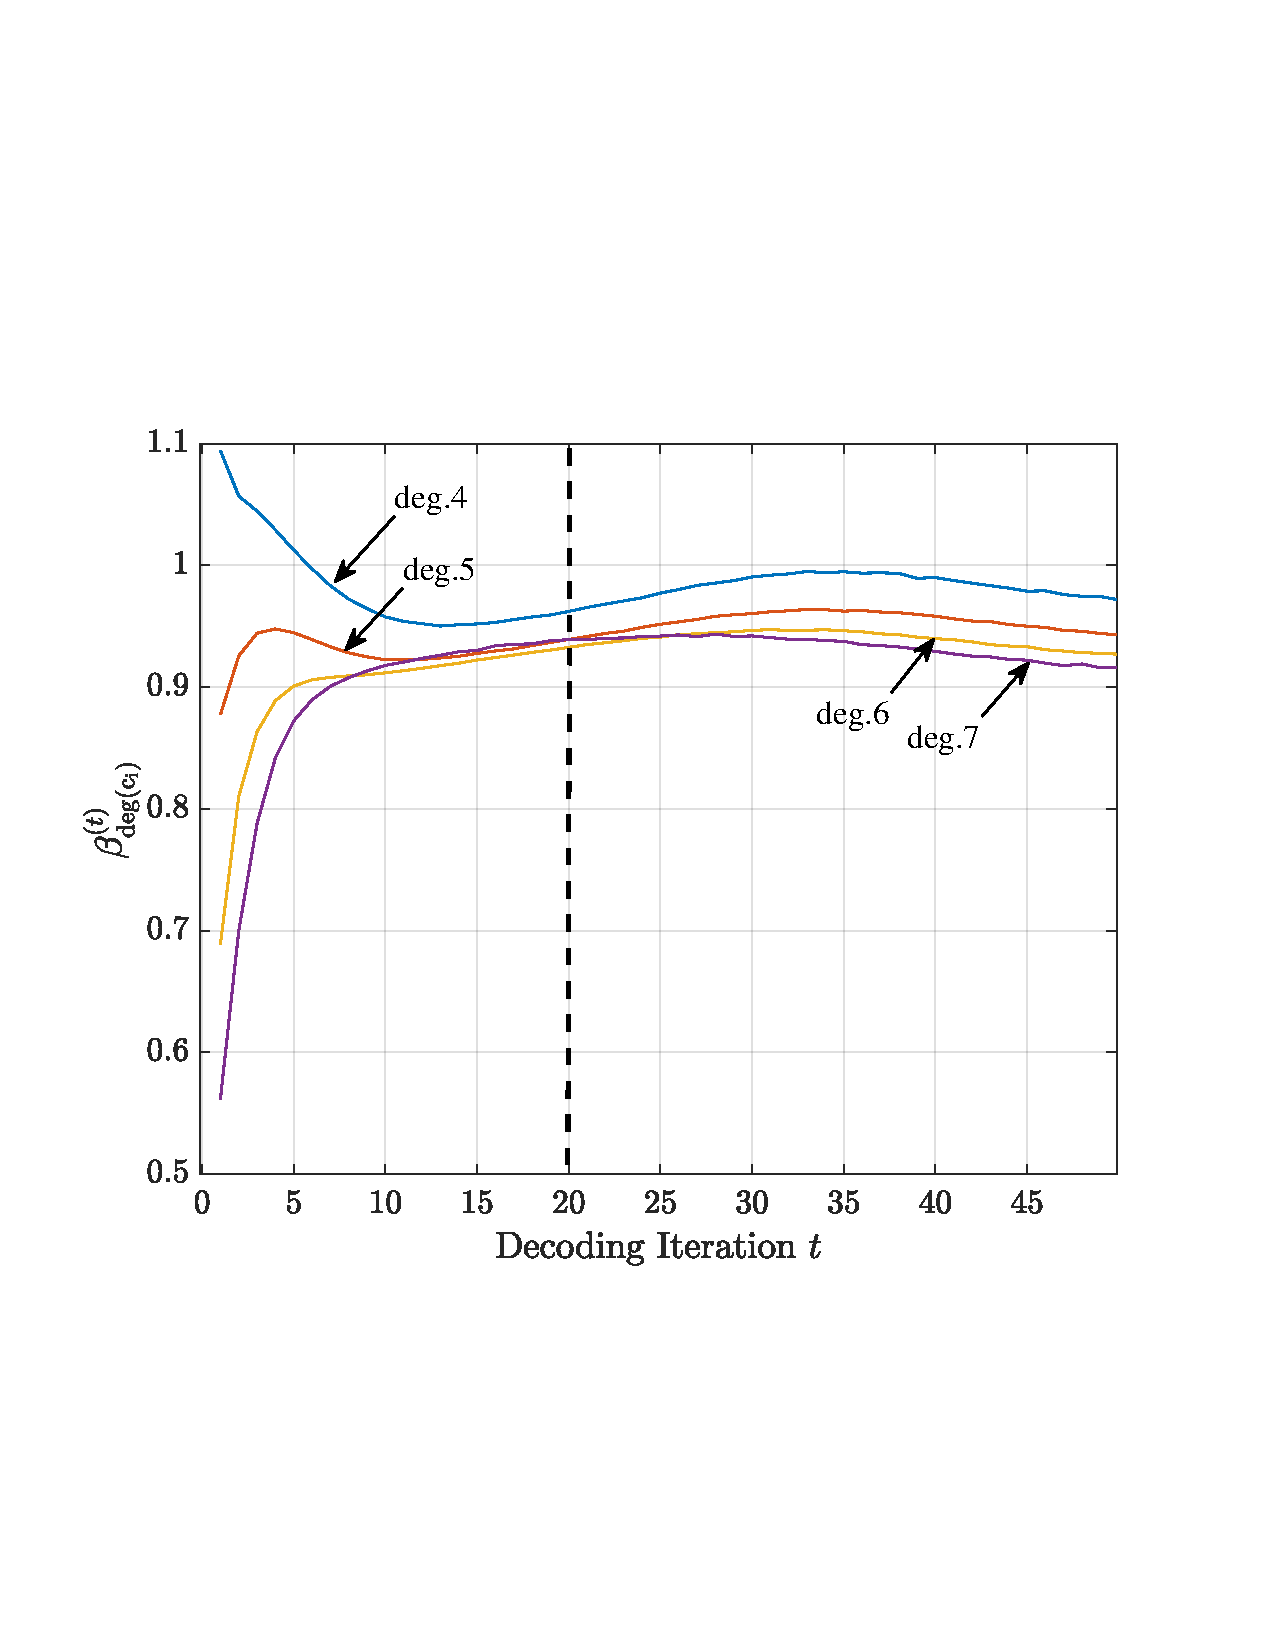
\includegraphics[width=0.50\linewidth]{figures/Fig_6_a_beta_iter.pdf}}
  \\
  \subfloat[\label{fig: alpha_iter}]{%
        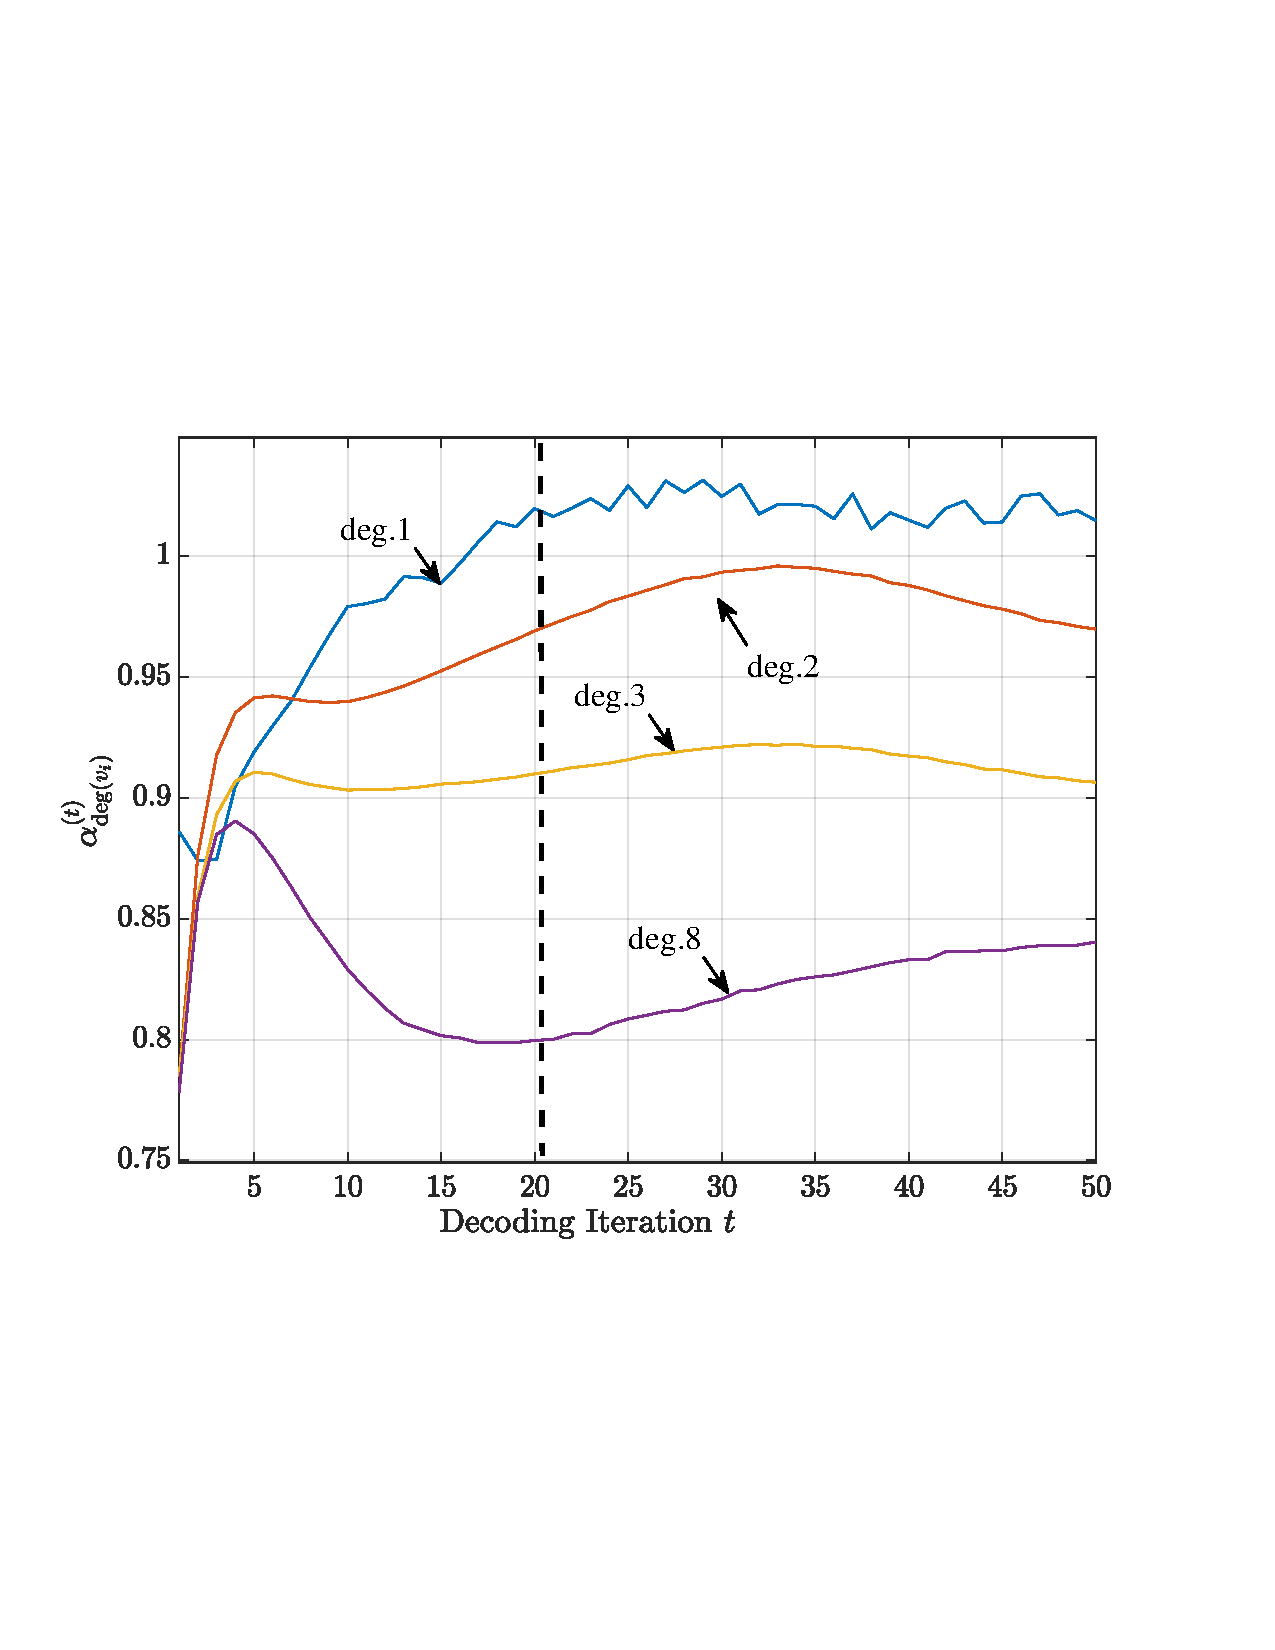
\includegraphics[width=0.50\linewidth]{figures/Fig_6_b_alpha_iter.pdf}}
  \caption{ The change of weights of the type-2 N-2D-NMS decoder for (16200, 7200) DVBS-2 LDPC code w.r.t. check node degree, variable node degree and iteration index.
  Specifically, Fig. (a) gives $\beta^{(t)}_{(\text{deg}({c_i}))}$ for all possible check node degrees in each decoding iteration $t$, Fig. (b) gives $\alpha^{(t)}_{(\text{deg}({v_j}))}$ for all possible variable node degrees in each decoding iteration $t$.}
\end{figure}

\subsection{(16200,7200) DVBS-2 LDPC code}
Fig. \ref{fig: dvbs2-fer} shows the FER performances of N-2D-NMS decoders with various weight sharing types for the (16200, 7200) DVBS-2 LDPC code. 
The FER performance of BP and NMS decoders are also given for comparison.  The single multiplicative weight of  NMS decoder is 0.88.
All of the decoders are flooding-scheduled and maximum decoding iteration is 50. 
It is shown that the N-NMS decoder (i.e., type-0 decoder) outperforms BP at $1.3$ dB with a lower error floor. The type-1 and 2 decoders, which share weights based on the check node and variable node degree, deliver even a slightly better decoding performance than N-NMS decoder.

Fig. \ref{fig: dvbs2-fer} also shows that the FER performance degrades if only considering to sharing weights w.r.t. check node degree (type-3) or variable node degree (type-4). Specifically, in this example, type-4 N-2D-NMS decoder outperforms type-3 N-2D-NMS decoder, because the variable node weights of investigated code have a larger dynamic range than check node weights, as shown in Fig. \ref{fig: beta_iter}, and \ref{fig: alpha_iter}. Fig. \ref{fig: beta_iter} and \ref{fig: alpha_iter} give the $\beta^{(t)}_{(\text{deg}({c_i}))}$ and $\alpha^{(t)}_{(\text{deg}({v_j}))}$ of type-2 N-2D-NMS decoder, which agree with our observation in the previous section; i.e., in each decoding iteration, larger degree node corresponds to a smaller value. Besides, as shown in Fig. \ref{fig: beta_iter} and \ref{fig: alpha_iter}, the  weights change negligibly after $20^{th}$ iteration. Thus, the hybrid type-2 N-2D-NMS decoder with $I'=20$ delivers similar performance to the full feed forward decoding structure, as shown in Fig. \ref{fig: dvbs2-fer2}. 

\begin{figure}[hp] 
    \centering
  \subfloat[\label{fig: fer_8k_1}]{%
       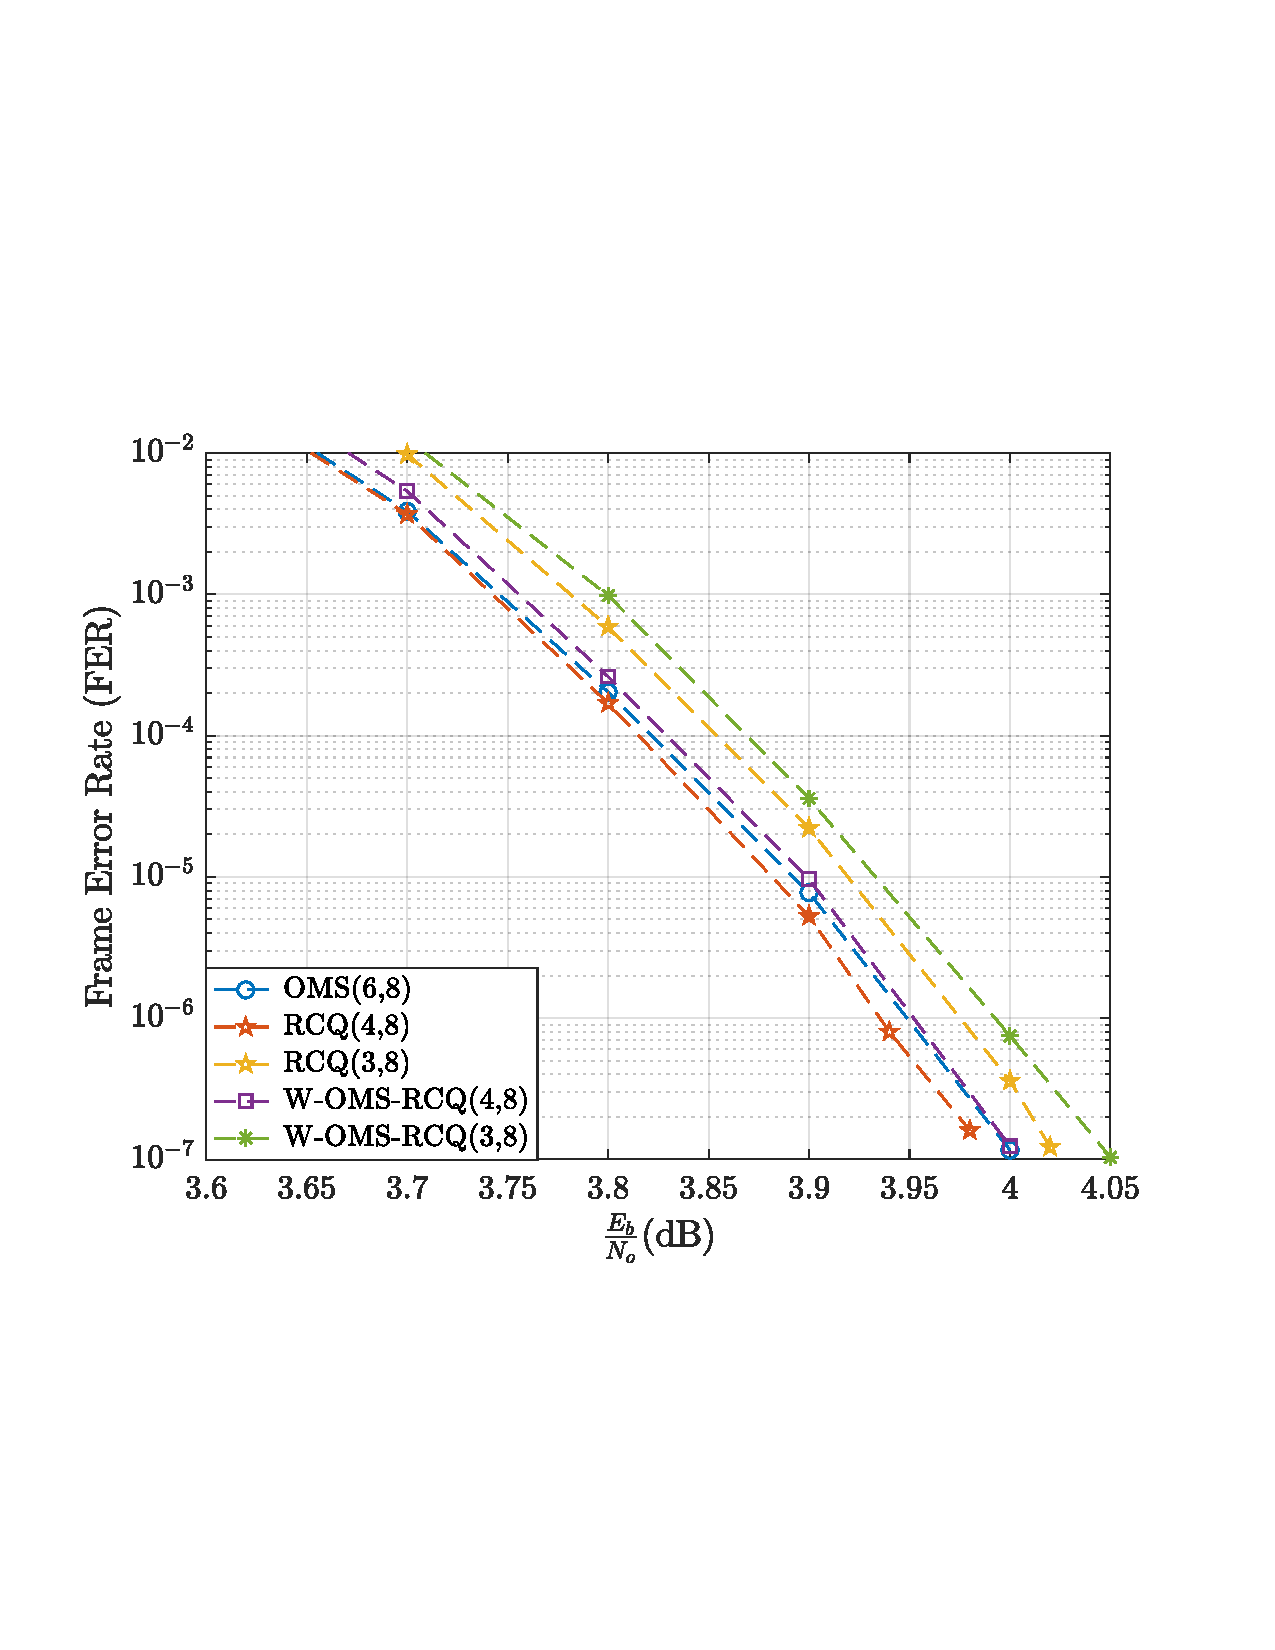
\includegraphics[width=0.50\linewidth]{figures/Fig7_a_8k_1.pdf}}
  \\
  \subfloat[\label{fig: fer_8k_2}]{%
        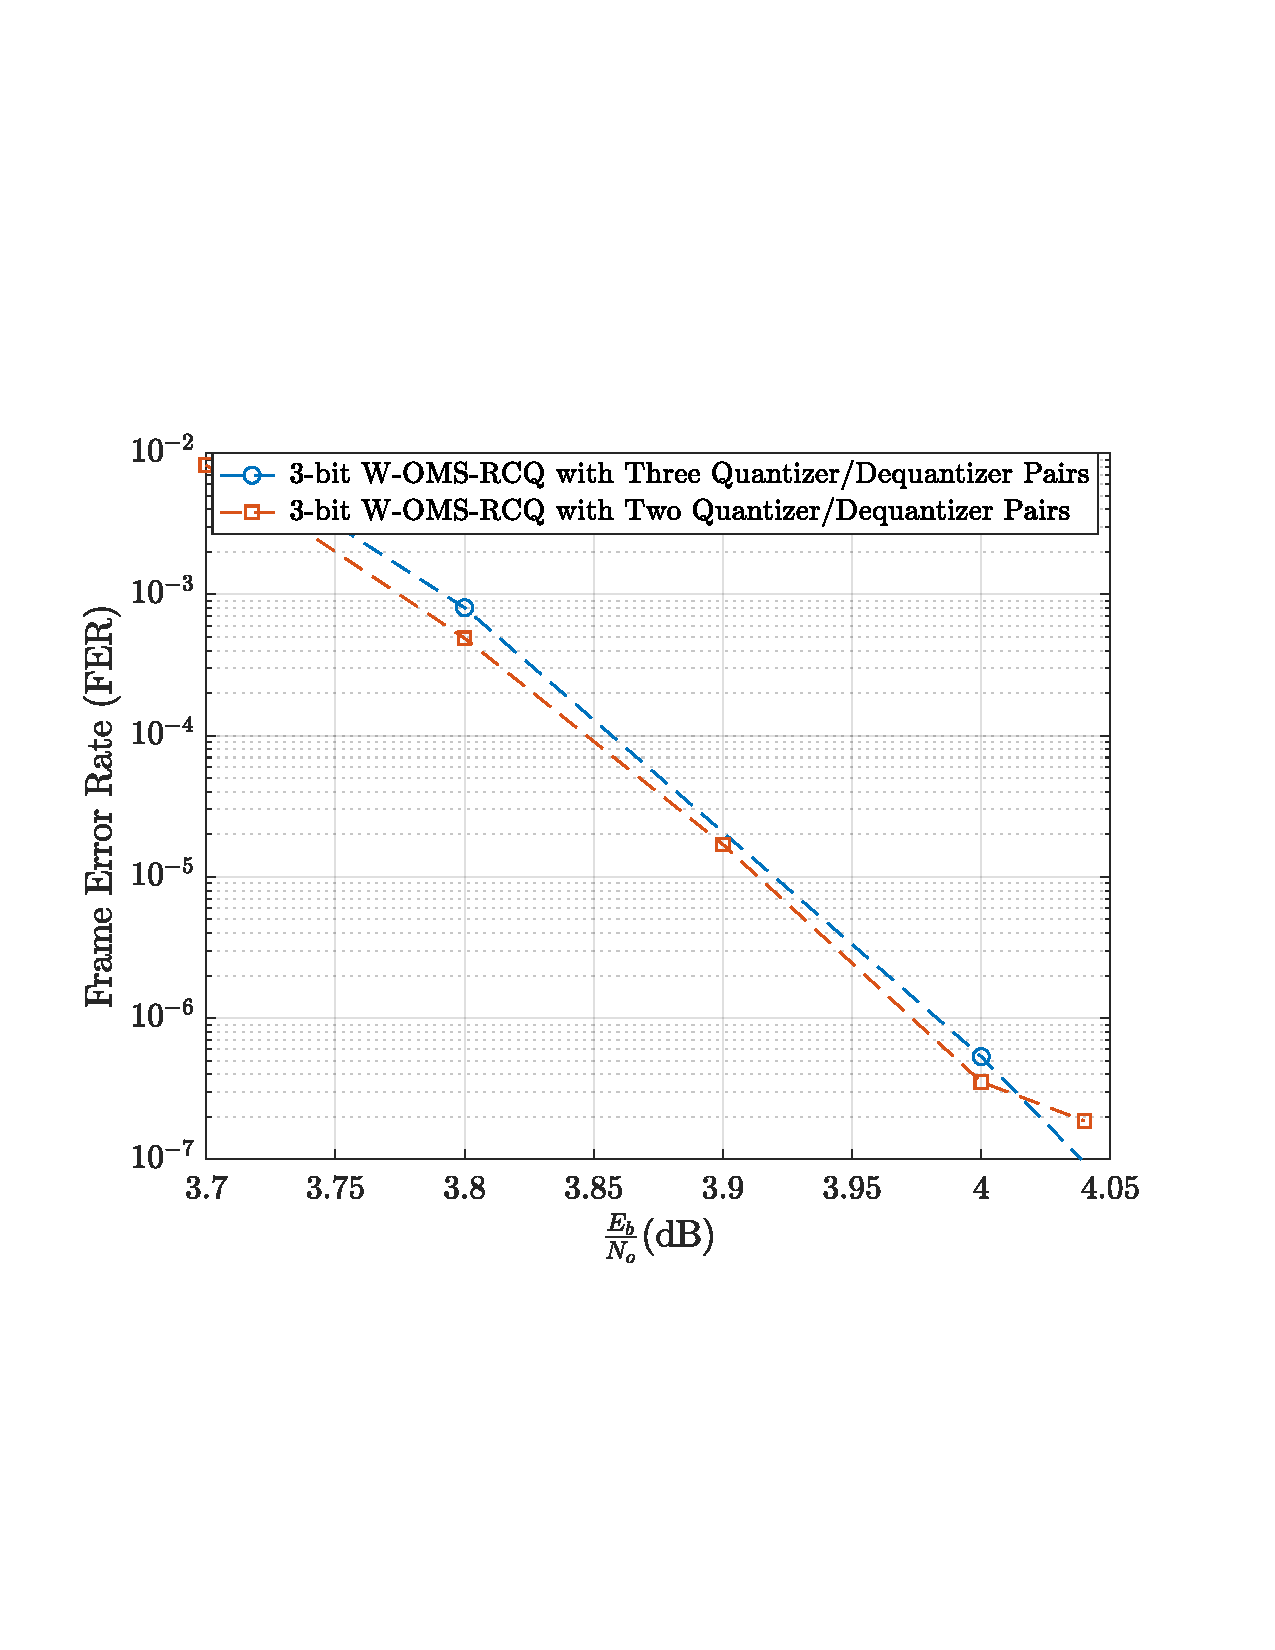
\includegraphics[width=0.50\linewidth]{figures/Fig7_a_8k_2.pdf}}
  \caption{Fig. (a): FER performance of W-OMS-RCQ decoders, RCQ decoders, and 6-bit OMS decoder for a (9472, 8192) QC LDPC code. Fig. (b): FER performance of 3-bit W-OMS-RCQ decoders with two and three quantizer/dequantizer pairs. Simulation result shows that the W-OMS-RCQ decoder with two quantizer/dequantizer pairs has an error error floor at FER of $10^{-7}$. }
\end{figure}

% Please add the following required packages to your document preamble:
% \usepackage{multirow}
\begin{table}[t]
    \centering
    \caption {The Quantizer/Dequantizer pairs of W-OMS-RCQ decoder for (9472,8192) LDPC code}
    \label{tab: 8k_config}
    \begin{tabular}{|c|c|c|}
    \hline
     CN bitwidth             & Quantizer/Reconstruction Parameter & Corresponding Decoder Iteration \\ \hline
    4 bits                  & $C=7$, $\gamma=1.7$                                                                       & $1\sim10$                                                                        \\ \hline
    \multirow{3}{*}{3 bits} & $C_1=3$, $\gamma_1=1.3$                                                                     & $1\sim6$                                                                         \\ \cline{2-3} 
                            & $C_2=5$, $\gamma_2=1.3$                                                                    & $7\sim8$                                                                         \\ \cline{2-3} 
                            & $C_3=7$, $\gamma_3=1.3$                                                                      & $9\sim10$                                                                        \\ \hline
    \end{tabular}
    \end{table}

\subsection{(9472,8192) Quasi-Cyclic LDPC code}
This subsection designs 3-bit and 4-bit W-OMS-RCQ decoders  for a (9742,8192) quasi-cyclic (QC) LDPC code  and compares them with the fixed-point OMS decoder and RCQ decoders. All decoders in this subsection are layer-scheduled with maximum iteration 10. The quantizer/reconstruction parameters for the 3-bit and 4-bit W-OMS-RCQ decoder are given in Table. \ref{tab: 8k_config}.

Fig. \ref{fig: fer_8k_1} compares the FER performances of W-OMS-RCQ decoders with RCQ decoders and a 6-bit OMS decoder. The decoders in Fig. \ref{fig: fer_8k_1} are also implemented using an FPGA device (Xilinx Zynq
UltraScale+ MPSoC) the study of resource usage. Table \ref{tab: hardware_usage} lists the usage of lookup tables (LUTs), registers, block RAM (BRAM), and routed nets of various decoders. For the details of FPGA implementations of the decoders, we refer the readers to \cite{terrill2021fpga}. 

Simulation result shows the 6-bit OMS decoder has the best FER performance. The 4-bit W-OMS-RCQ decoder and 4-bit RCQ decoder have similar FER performance, which are inferior to the 6-bit OMS decoder by 0.015 dB. However, as shown in Table \ref{tab: hardware_usage}, the 4-bit W-OMS-RCQ decoder requires much less resources compared with the 4-bit RCQ decoder and the 6-bit OMS decoder. Compared to the 6-bit OMS decoder, the 3-bit W-OMS-RCQ and 3-bit RCQ decoder have a gap of 0.04 and 0.06 dB, respectively. More specifically, the 3-bit RCQ decoder has a similar LUT, BRAM and routed net usage to the 4-bit W-OMS-RCQ decoder. On the other hand, the 3-bit W-OMS-RCQ uses much fewer resource than the 4-bit W-OMS-RCQ decoder.


\begin{table}[t]
    \small
    \caption{\label{tab: hardware_usage} Hardware Usage of Various Decoding Structure for (9472,8192) QC-LDPC Code }
    \centering
    \begin{tabular}{|c|c|c|c|c|}
    \hline
    Decoding Structure  & LUTs                                            & Registers                                       & BRAMS                                           & Routed Nets                                     \\ \hline
    OMS(6,8) (baseline) & 21127                                           & 12966                                           & 17                                              & 29202                                           \\ \hline
    RCQ(4,8)          & 20355(\textcolor{mygreen}{$\downarrow 3.6\%$} ) & 13967(\textcolor{red}{$\uparrow 7.0\%$})        & 17.5(\textcolor{red}{$\uparrow .03\%$})         & 28916(\textcolor{mygreen}{$\downarrow 1\%$})    \\ \hline
    RCQ(3,8)          & 17865(\textcolor{mygreen}{$\downarrow 15.4\%$}) & 12098(\textcolor{mygreen}{$\downarrow 6.7\%$})  & 17(\textcolor{blue}{$-$})                       & 25332\textcolor{mygreen}{($\downarrow 13.3\%$}) \\ \hline
    W-OMS-RCQ(4,8)         & 17645(\textcolor{mygreen}{$\downarrow 16.5\%$} ) & 13297(\textcolor{red}{$\uparrow 2.6\%$}) & 17(\textcolor{blue}{$-$}) & 25361(\textcolor{mygreen}{$\downarrow 13.2\%$} )\\ \hline
    W-OMS-RCQ(3,8)         & 16306(\textcolor{mygreen}{$\downarrow 22.82\%$} ) & 12104(\textcolor{mygreen}{$\downarrow 6.65\%$}) & 17(\textcolor{blue}{$-$}) & 23252(\textcolor{mygreen}{$\downarrow 20.38\%$} )\\ \hline
    \end{tabular}
    \end{table}

Fig. \ref{fig: fer_8k_1} compares the FER performances of W-OMS-RCQ decoders with RCQ decoders and a 6-bit OMS decoder. The decoders in Fig. \ref{fig: fer_8k_1} are also implemented using an FPGA device (Xilinx Zynq
UltraScale+ MPSoC) the study of resource usage. Table \ref{tab: hardware_usage} lists the usage of lookup tables (LUTs), registers, block RAM (BRAM), and routed nets of various decoders. For the details of FPGA implementations of the decoders, we refer the readers to \cite{terrill2021fpga}. 

Simulation result shows the 6-bit OMS decoder has the best FER performance. The 4-bit W-OMS-RCQ decoder and 4-bit RCQ decoder have similar FER performance, which are inferior to the 6-bit OMS decoder by 0.015 dB. However, as shown in Table \ref{tab: hardware_usage}, the 4-bit W-OMS-RCQ decoder requires much less resources compared with the 4-bit RCQ decoder and the 6-bit OMS decoder. Compared to the 6-bit OMS decoder, the 3-bit W-OMS-RCQ and 3-bit RCQ decoder have a gap of 0.04 and 0.06 dB, respectively. More specifically, the 3-bit RCQ decoder has a similar LUT, BRAM and routed net usage to the 4-bit W-OMS-RCQ decoder. On the other hand, the 3-bit W-OMS-RCQ uses much fewer resource than the 4-bit W-OMS-RCQ decoder.

The 3-bit W-OMS-RCQ decoder in Fig. \ref{fig: fer_8k_1} uses three quantizers for three decoding phases. In the first 3 iteration, most messages have low magnitudes, hence a quantizer with small $C$ is required for a finer resolution to the low-magnitude values. However, the message magnitudes increase with the increase of decoding iteration. As a result, the quantizers with larger $C$ should be used correspondingly. Fewer quantizers may not accommodate the message magnitude growth in the decoding process and will result in performance degradation. For example, Fig. \ref{fig: fer_8k_2} considers a 3-bit W-OMS-RCQ decoder that uses two quantizer/dequantizer pairs, the first pair has $C_1=3$, $\gamma_1=1.3$ and is used for iteration $1\sim7$, the second pair has $C_2=5$, $\gamma_2=1.3$ and is used for iteration $8\sim10$. Simulation result shows that the 3-bit W-OMS-RCQ decoder that uses 2 quantizer/dequantizer pairs has an early error floor at FER of $10^{-7}$.
\begin{figure}[t]
	\centering
	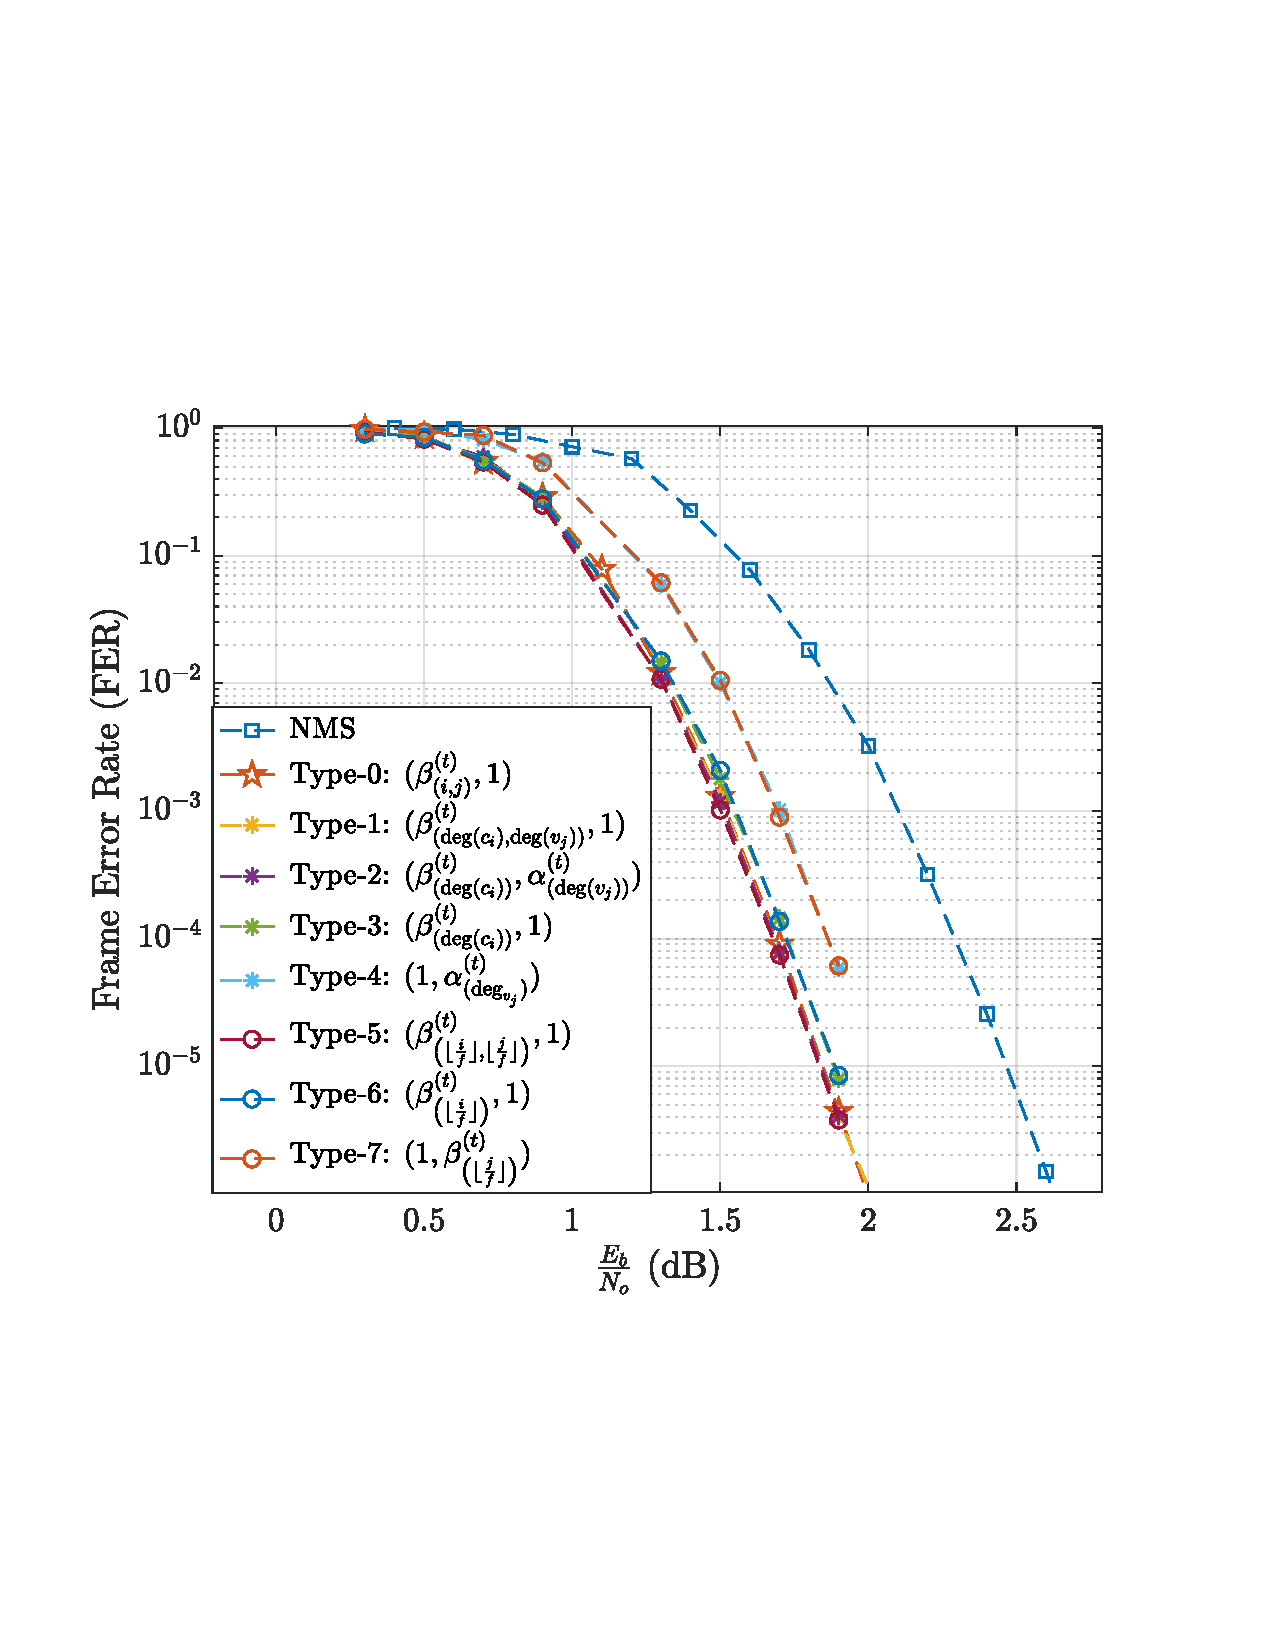
\includegraphics[width=0.5\linewidth]{figures/Fig8_N2DNMS_PBRL.pdf}  
	\caption{FER performance of N-2D-NMS decoders with various weight sharing types for a (3096,1032) PBRL LDPC code compared with N-NMS (type 0) and NMS.}
    \label{fig: FER1}
\end{figure}

subsection{$k=1032$ Protograph-Based Raptor-Like code}

5G LDPC codes have the protograph-based raptor-like (PBRL) \cite{PBRL} structure which offers inherent rate-compatibility and excellent decoding performance. In this subsection, we examine the performance of N-2D-NMS decoders and W-RCQ decoders for a $k=1032$ PBRL LDPC code, whose supported rates are listed in Table \ref{tab:weight_sharing}.  The edge distribution of the lowest-rate code, which corresponds to the full parity check matrix, is also given in Table \ref{tab:weight_sharing}.  All the decoders in this subsection are layer-scheduled with maximum 10 decoding iterations. 

\begin{figure}[hp] 
    \centering
  \subfloat[\label{fig: pbrl_fer_1}]{%
       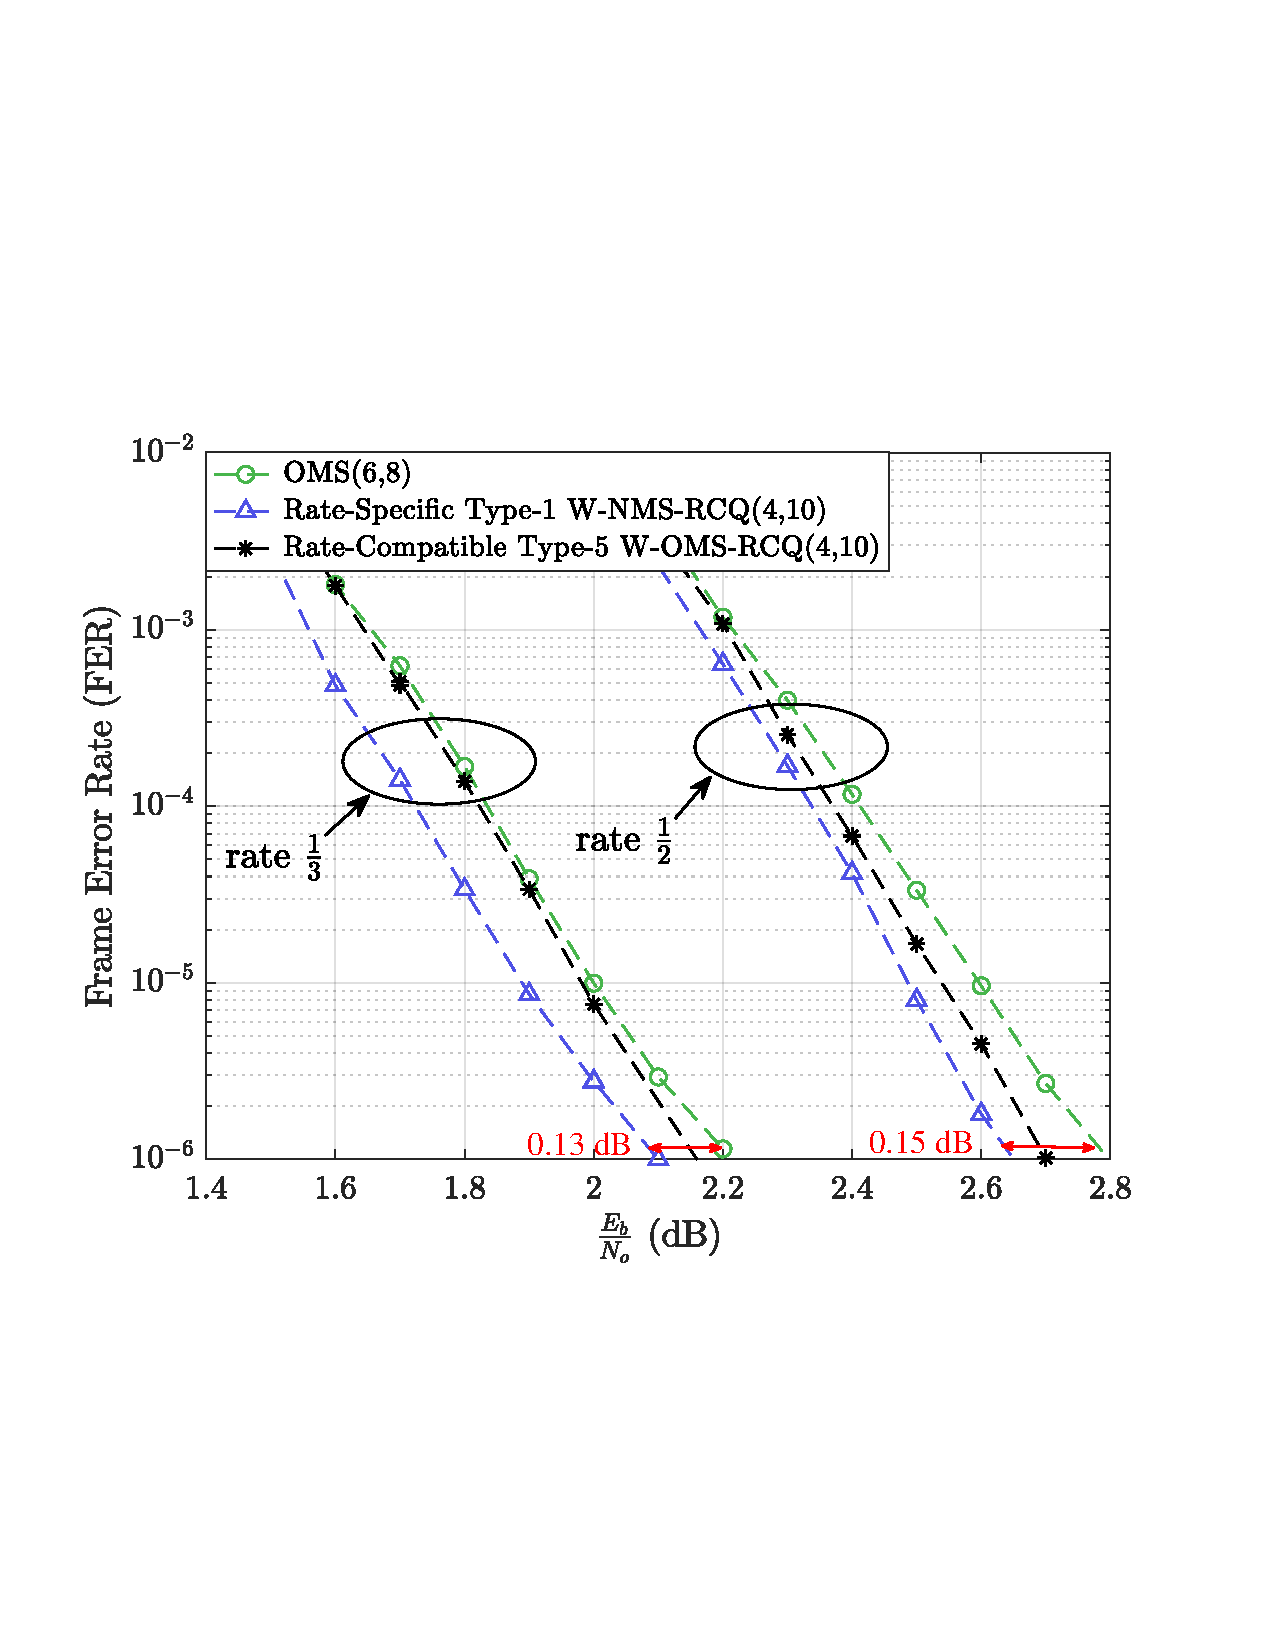
\includegraphics[width=0.50\linewidth]{figures/Fig_9_a_rate_13_12.pdf}}
  \\
  \subfloat[\label{fig: pbrl_fer_2}]{%
        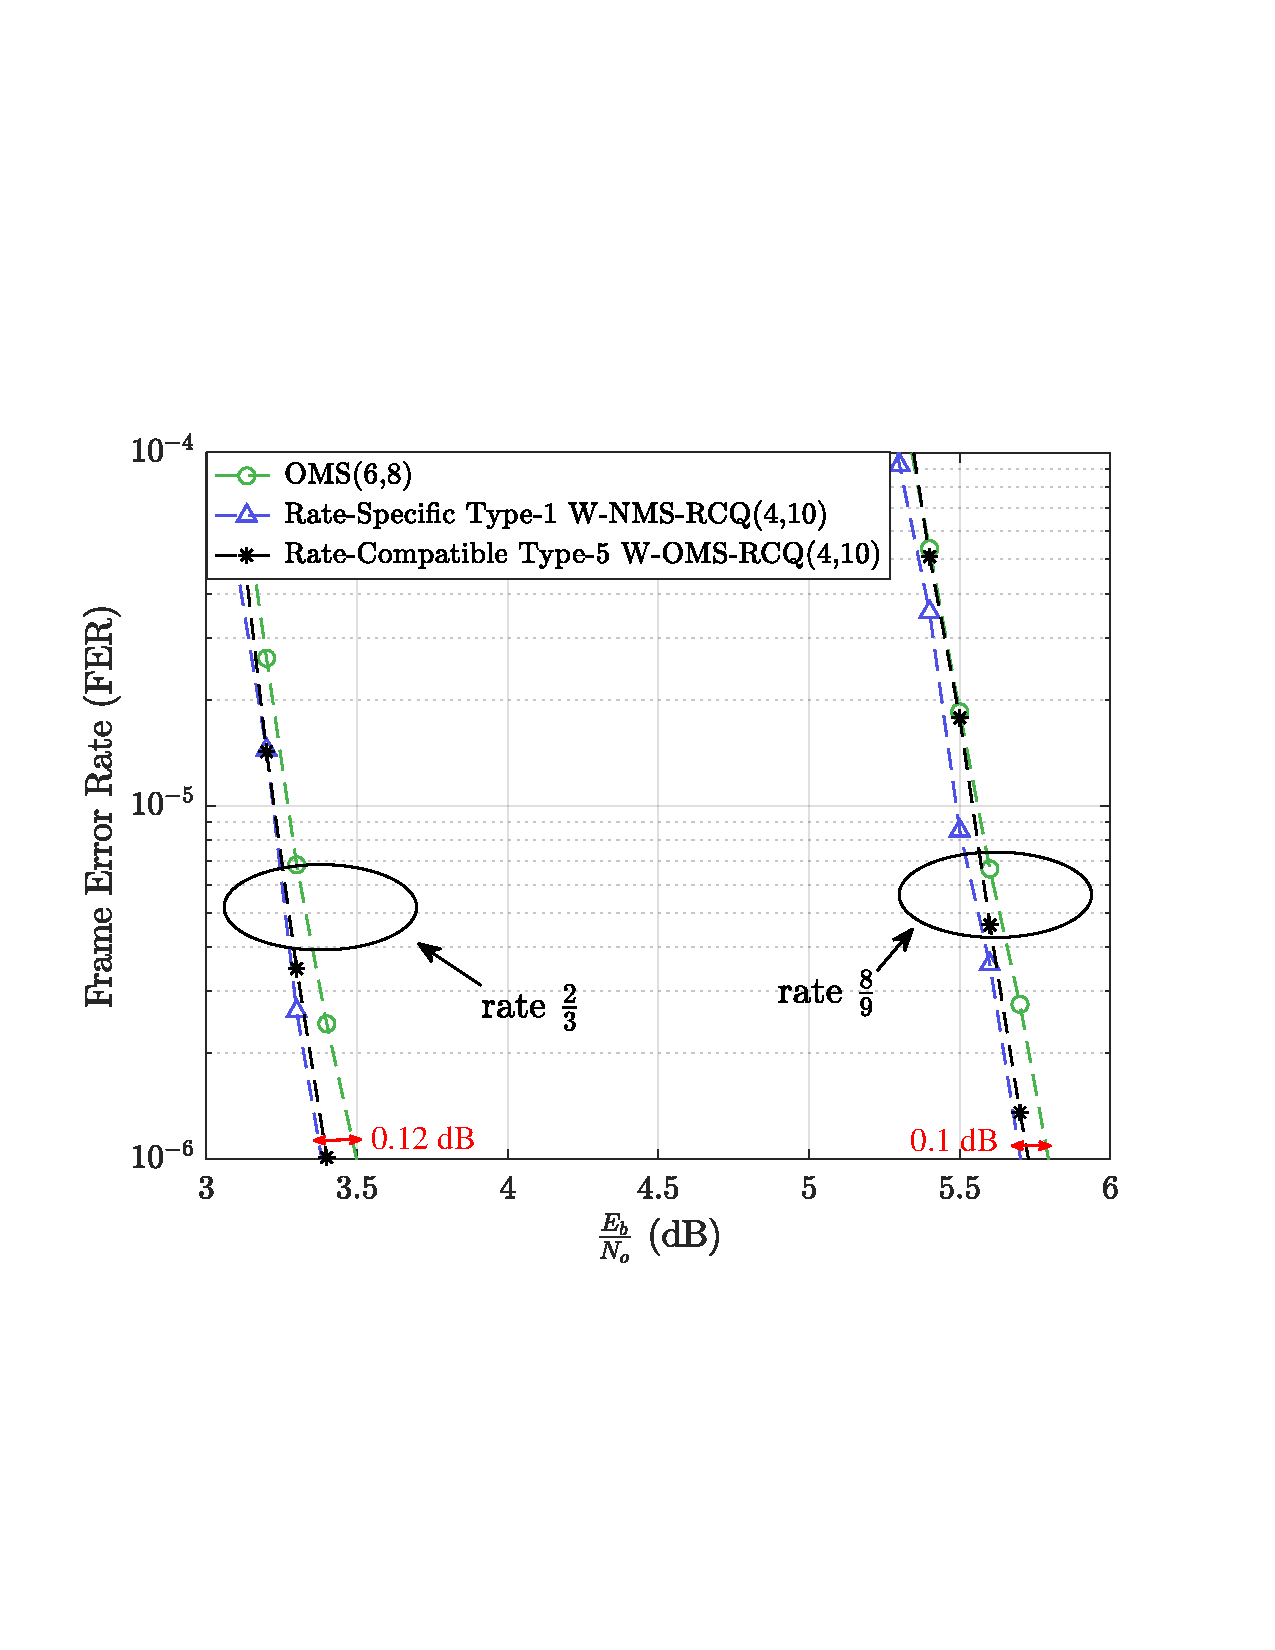
\includegraphics[width=0.50\linewidth]{figures/Fig_9_a_rate_23_89.pdf}}
  \caption{FER performance of 4-bit W-RCQ decoders for $k=1032$ PBRL code with different code rates. The term "rate-specific" means to design distinct decoders for each code rate; The term "rate-compatible" means to train one decoder that matches all code rates. The 6-bit OMS decoder is given as comparison. }\label{fig: pbrl}
\end{figure}


Fig. \ref{fig: FER1} shows the FER performance of  N-2D-NMS decoder with various weight sharing types for the PBRL code with lowest code rates $\frac{1}{3}$. As a comparison, the decoding performance of the N-NMS (type 0) decoder and the NMS decoder are also given. All of the decoders use floating-point message representation. The simulation results show that N-NMS decoder has a more than 0.5 dB improvement over the NMS decoder. N-2D-NMS decoders with weight sharing types 1-7  are also simulated. 
%The number of parameters of N-NMS and N-2D-NMS decoders in each iteration are presented in  
%The types 1, 2 and 5 have the same decoding performance as the N-NMS decoder, with parameter reduction by 99.7\%, 99.9\% and 99.3\%, respectively. 
Simulation result shows that the N-2D-NMS decoders with weight-sharing metrics based on check and variable node degree (i.e., type 1 and 2), or based on horizontal and vertical layer  (i.e., type 5) deliver lossless performance w.r.t. N-NMS decoder.  N-2D-NMS decoders with weight sharing types 4 and 6 have a degradation of around 0.05 dB compared with the N-NMS decoder.  N-2D-NMS decoders with weight sharing types 5 and 7 have a degradation of around 0.2 dB compared with the N-NMS decoder. Thus, for this (3096,1032) PBRL LDPC code of Fig. \ref{fig: FER1}, assigning weights based only on check nodes can gain more benefit than assigning weights only based on variable nodes.



Fig. \ref{fig: pbrl} gives the FER performance of fixed-point W-NMS-RCQ decoders for the $k=1032$ PBRL code with rate $\frac{1}{3}$, $\frac{1}{2}$, $\frac{2}{3}$ and $\frac{8}{9}$. The W-NMS-RCQ decoder assigns 4 bits to C2V message and 10 bits to V2C message. Two quantizer/dequantizer pairs are used for W-NMS-RCQ decoder across all investigated rates.
The first quantizer has $C_1=7$, $\gamma_2=1.7$ and is used for the first 7 iterations. The second quantizer has $C_2=10$, $\gamma_2=2.3$ and is used for last 3 iterations.
We use a 6-bit OMS decoder as benchmark, because we find it delivers a better decoding performance than the NMS decoder with same bit width.
Additionally, we didn't consider W-OMS-RCQ decoder for this code because the 4-bit W-OMS-RCQ decoder doesn't perform as well as the 4-bit W-NMS-RCQ decoder. 

We first consider the 4-bit W-NMS-RCQ decoder with type-1 weight sharing that assigns the same weight to the edges with same check and variable node degree.
The decoder is rate-specific; i.e., for each considered rate, a W-NMS-RCQ decoder is trained separately.
The simulation results shows that, targeting a FER of $10^{-6}$, the 4-bit rate-specific W-NMS-RCQ decoder outperforms the 6-bit OMS decoder with 0.1$\sim$ 0.15 dB for all considered code rates.

For the PBRL code, the proto-matrix of each possible rate is a sub-matrix of a base proto-matrix \cite{PBRL}. As shown in Table. \ref{tab:weight_sharing}, the type-5 weight sharing assigns the same weight to the edges that correspond to the same element in the proto-matirx. Hence, it is possible to use \emph{one} trained type-5 neural decoder to match different code rates. We refer to such decoder as a rate-compatible decoder. In \cite{dai2021learning}, the authors propose to training the rate-compatible decoder by using the samples from different code rates. 

Fig. \ref{fig: pbrl} shows the decoding performance of rate-compatible type-5 W-NMS-RCQ decoder. Simulation result shows that for the higher rate such as $\frac{2}{3}$ and $\frac{8}{9}$, the rate-compatible type-5 W-NMS-RCQ decoder has a similar decoding performance to the rate-specific type-1 W-NMS-RCQ decoder whose parameters for each rate  are separately designed.  However, for the lower rate such as $\frac{1}{3}$ and $\frac{1}{2}$, the rate-compatible type-5 W-NMS-RCQ decoder method doesn't deliver a decoding performance as well as rate-specific type-1 W-NMS-RCQ decoder.
Besides, considering the four rates in Fig. \ref{fig: pbrl}, the number of neural weights for rate-specific type-1 and rate-compatible type-5  W-NMS-RCQ decoder are 96 and 101, respectively.

\section{Conclusion}\label{sec: conclusion_c2}
This chapter proposes the W-RCQ decoder, a non-uniformly quantized decoder that delivers excellent decoding performance in the low-bitwidth regime.
%Compared with RCQ decoder, W-RCQ decoder uses fewer parameters and provides comparable decoding performance. 
Unlike RCQ decoder, which designs quantizer/dequantizer pairs for each layer and iteration, W-RCQ decoder only uses a small number of quantizer/dequantizer pairs and each one is responsible for several iterations. 
The W-RCQ decoder uses Min operation at check node, and the C2V messages are weighted by multiplicative or additive parameters, which induce W-NMS-RCQ and W-OMS-RCQ, respectively. 

For the neural decoders such as W-RCQ decoder and N-NMS decoder, assigning distinct weights to each edge in each decoding iteration is impractical for long-blocklength codes because of huge number of neural weights.
This paper proposes various node-degree-based weight sharing schemes with  lossless or lossy performance for the neural decoders, depending on whether the weight sharing considers both check and variable node degree or only one of them. 

Additionally, this paper discusses the issues when training neural LDPC decoders. First, training the neural LDPC decoders for long blocklength code using Pytorch or TensorFlow could raise memory issue. This paper shows that the memory for training neural MinSum decoders can be saved by storing feed-forward messages compactly. Second, this paper identifies gradient explosion problem in the neural decoder training and proposes a  posterior jointly training method that addresses this problem. 


\chapter{Probabilistic Shaping for Trellis-Coded Modulation with CRC-Aided List Decoding} \label{cpt: CRC_TCM_PAS}

\section{Introduction}
This paper explores reliable communications over the additive white Gaussian noise (AWGN) channel with high spectral efficiency for short block lengths.  To closely approach theoretical limits, it is helpful to use shaping so that signal points are not equally likely, not equally spaced, or both \cite{gallager1968information,ForneyShaping,forney1992trellis,Kschischangoptimaldist,laroia1994optimal,fragouli2001,xiao2021finite}.  Recently, a new technique called  probabilistic amplitude shaping (PAS) \cite{pas_bocherer_1,pas_bocherer_2} employs a distribution matcher (DM) \cite{CCDM_schulte} before the forward error correction (FEC) encoder and channel-signaling mapping function to accomplish optimal or almost optimal shaping.

A PAS system as in \cite{pas_bocherer_1,pas_bocherer_2} decomposes a channel input sequence into a magnitude symbol sequence and a sign sequence. The magnitude symbol sequence is generated by a DM.  The output of the DM is provided as input to a systematic FEC code where the parity check bits indicate the signs of the channel inputs. A channel-signaling mapping function maps the amplitude symbol sequence and the sign-bit sequence to the corresponding sequence of transmitted signal points.

A distribution matcher \cite{CCDM_schulte,SMDM_amjad,ccdm_smdm_comp_schulte,patrick,pikus2019arithmetic,fehenberger2018multiset} maps a binary  input sequence onto a symbol sequence that determines the magnitudes of the transmitted symbols. The  binary input sequence typically has equally likely ones and zeros. However, the output symbols from  the distribution matcher are not equally likely. Specifically, the distribution matcher is designed such that the PAS system can generate channel inputs with a capacity-approaching probability mass function (PMF). 

Even though it is well-known that 
a continuous Gaussian probability density function (PDF) is a
capacity-achieving distribution for the power-constrained additive Gaussian white noise (AWGN) channel, a carefully designed  finite-cardinality PMF  can deliver performance that is almost indistinguishable from that of a Gaussian PDF and facilitates practical implementation.  In \cite{Kschischangoptimaldist}, Kschischang \emph{et. al.} use Maxwell-Boltzmann distribution to optimize the PMF of equally-spaced pulse-amplitude modulation (PAM) or quadrature amplitude modulation (QAM) constellations. Xiao \emph{et. al.} use dynamic Blahut-Arimoto (DAB) to identify  minimum-cardinality capacity-approaching input PMFs for PAM constellations\cite{xiao2021finite}. 
%Because the optimal channel input distribution is symmetric, the magnitude distribution can be calculated correspondingly.
\begin{figure*}[t]
    \centering
    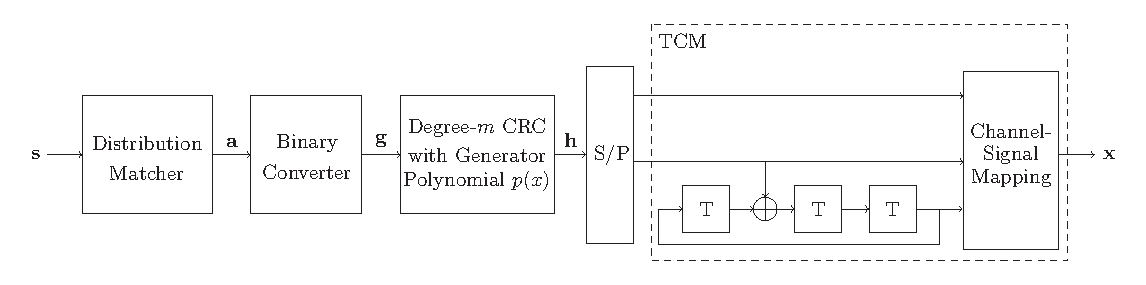
\includegraphics[width=1\linewidth]{figures/CRC_TCM_PAS_v2.eps }
    \caption{Diagram of the CRC-TCM-PAS transmitter. In the diagram, $\mathbf{s}\in\mathbb{F}_2^{k}$, $\mathbf{a}\in\mathcal{C}_{\mathrm{DM}}\subseteq\mathcal{A}^{\length}$, $\mathbf{g}\in\mathbb{F}_2^{\ccinnum \length}$,   $\mathbf{h}\in\mathbb{F}_2^{\ccinnum \length+m}$, $\mathbf{x}\in\mathcal{X}^{\outlen}$, and $n=\length+\frac{m}{\ccinnum}$. The transmission rate of the system is $\frac{k}{n}$ bits/real channel use. The TCM in this figure uses a rate-$\frac{2}{3}$ TBCC.}
    \label{fig: transmitter}
\end{figure*}


The empirical distribution of the output symbols of a good distribution matcher will closely resemble the target PMF as determined, for example, according to \cite{xiao2021finite}. The shell-mapping (SM) DM  \cite{SMDM_amjad,ccdm_smdm_comp_schulte}  is optimal in termes of normalized Kullback-Leibler (KL) divergence.  Schulte \emph{et al.} in \cite{CCDM_schulte} propose an asymptotically optimal distribution matcher, the constant composition (CC) DM. 
One advantage of CCDM is that it supports online encoding. 
Some other distribution matchers include those of  \cite{patrick,pikus2019arithmetic,fehenberger2018multiset}.

As in \cite{pas_bocherer_1,pas_bocherer_2}, the output of the distribution matcher is provided as input to a systematic FEC code where the parity check bits indicate the signs of the channel inputs. The channel-signaling mapping function maps the amplitude-bit sequence of the DM and the sign-bit sequence of the FEC to the corresponding sequence of transmitted signal points.

The second module in the PAS transmitter is a coded modulator. Coded modulation is a combination of error correction code and modulation. A well know coded modulation is Underboeck's trellis-coded modulation (TCM)\cite{ungerboeck1982channel}.   The coded modulation in the PAS transmitter \cite{pas_achievablerate_bocherer} comprises a systematic error correction code and a channel-signal mapping function.

An important design choice for a PAS system is the selection of an FEC code. In the long blocklength regime, B{\"o}cherer \emph{et. al.} in \cite{pas_bocherer_1} use low-density parity-check (LDPC) codes for the PAS system. In the short blocklength regime, Coşkun \emph{et. al.} in \cite{cocskun2019efficient} investigate PAS systems with various FEC choices including binary LDPC codes, non-binary LDPC codes and polar codes. 

Recently, convolutional codes with cyclic redundancy code (CRC)-aided list decoding have shown excellent performance in the short blocklength regime \cite{Liang_tbcccrc,yang2018serial,yang2019list,9709319}. Yang \textit{et al.} in \cite{Liang_tbcccrc} show that a tail-biting convolutional code (TBCC) with CRC-aided list decoding can achieve frame error rate (FER) performance very close to the short-blocklength random coding union (RCU) bound \cite{polyrcu}. King.  \textit{et al.} in \cite{king2022crc} provide an example where a TBCC outperforms a polar code in the AWGN channel when both are decoded using CRC-aided list decoding.

\subsection{Contributions}

In this paper, we propose a PAS system designed for the AWGN channel in the short-blocklength regime. The proposed PAS system uses a CRC-aided, rate-$\frac{\ccinnum}{\ccinnum+1}$, systematic, recursive TBCC as the FEC code. The TBCC and the channel-signal mapping function constitute the TCM \cite{ungerboeck1982channel}.  
We refer to the proposed PAS system as CRC-TCM-PAS. Fig. \ref{fig: transmitter} describes the transmitter of the CRC-TCM-PAS  system.
A CRC-TCM-PAS system can be designed as follows:
\begin{enumerate}
    \item Using \cite{Kschischangoptimaldist} or \cite{xiao2021finite}, identify the capacity-approaching PMF for the PAM constellation under AWGN,  which induces the PMF for the corresponding magnitudes.
    \item Assuming an ideal distribution matcher that generates magnitude sequences whose symbols are independent and identically distributed (i.i.d.) according to the distribution calculated in 1), optimize the CRC and TBCC using the FER upper bound developed in Section \ref{sec:tfbound}. 
    \item Replace the ideal distribution matcher with a practical one.
\end{enumerate}
The contributions of this chapter are summarized as follows:
\begin{itemize}
    \item \textit{CRC-TCM-PAS transmission system.} This chpter presents the paradigm of the  CRC-TCM-PAS  system.
    \item \textit{Multi-composition distribution matcher (MCDM).} 
    MCDM, which can be seen as a collection of CCDMs, is proposed in this chapter. We note that the proposed distribution matcher is a generalization of the MCDM in \cite{MCDM}, which limits the cardinality of the output alphabet to 2. We investigate two rules to select the CCDMs, which are related to high-probability sets and typical sets in information theory.
    \item \textit{CRC-TCM-PAS  Decoder.} We propose automorphism enabled decoding \cite{geiselhart2022automorphism} to achieve near-maximum-likelihoood performance with low time complexity.
    \item \textit{Properties of CRC-TCM-PAS transmission system.} This chapter proves that, asymptotically, the sign values produced by the TCM are equally likely to be positive or negative. This yields channel input symbols that have a symmetric capacity-approaching distribution.
    \item \textit{Optimization of CRC-TCM-PAS parameters.} This chapter derives an upper bound on the FER of CRC-TCM-PAS systems and uses this bound as an objective function to jointly optimize the CRC and TBCC. The optimized CRC-TCM-PAS systems achieve FERs below the random coding union (RCU) bound in AWGN and outperform the short-blocklength PAS systems with various other forward error correction codes studied in \cite{cocskun2019efficient}. Simulation results show that the optimized CRC-TCM-PAS systems can exceed RCU bound and outperforms PAS systems with various other FEC codes explored in \cite{cocskun2019efficient}.
\end{itemize}

\subsection{Organization}
The remainder of this chapter is organized as follows: Section \ref{sec: DM} reviews CCDM and presents MCDM. 
The performance of these distribution matchers are compared in this section. 
Section  \ref{sec: Prop} presents CRC-TCM-PAS system architecture.  Section \ref{sec: property} proves the symmetric capacity-approaching distribution of the output of the CRC-TCM-PAS system. Section \ref{sec:tfbound} derives the FER upper bound, and Section \ref{sec: simu} presents the simulation results of CRC-TCM-PAS systems with different input lengths and transmission rates. Section  \ref{sec: conclusion_3} concludes our work.
 
\subsection{Notation}
In this chapter, we use the italic upper case letter $A$ to denote a random variable. We use $A^l=[A_1,\ldots,A_l]$ to denote a random vector. 
We use the italic lowercase letter $a$ to denote a realization of $A$ or a variable. 
We use the straight bold lowercase letter $\mathbf{a}$ to denote either a realization of $A^l$ or a column vector. Specifically, $[\mathbf{a}]_m$ is a vector that contains last $m$ elements in $\mathbf{a}$.   
Finally, we use the straight, bold upper case letter $\mathbf{A}$ to denote a matrix.

\subsection{Preliminaries}
Let $S$ be a random variable that obeys $\text{Bernoulli}\left(\frac{1}{2}\right)$, and  Denote the random sequence of $S$ with length $\numbits$ by $S^\numbits$, and the random sequence of $A$ with length $\length$ by $A^\length$. Specifically, $S^{\numbits}=[S_1,\dots,S_\numbits]$ and $A^{\length}=[A_1,\                               \dots,A_\length]$. Let $A$ be a random variable with alphabet $\mathcal{A}=\{0,1,\ldots,|\mathcal{A}|-1\}$.

A fixed-to-fixed  distribution matcher is an injective function $f_{DM}$ that maps a  binary length-$\numbits$ source sequence $\soursymsqe\in\mathbb{F}_2^{\numbits}$ to a length-$\length$ symbol sequence $\dmou\in\mathcal{A}^{\length}$, i.e., 
\begin{align}
    f_{DM}: \{0,1\}^\numbits\rightarrow \mathcal{A}^\length.
\end{align}
$\mathcal{A}=\{0,1,\ldots,|\mathcal{A}|-1\}$ is the output symbol set. In this chapter, we limit $\log_2|\mathcal{A}|=k$ to be some integer. 
The range of $f_{\mathrm{DM}}$ is the codebook of the distribution matcher, which is denoted by $\mathcal{C}_{\mathrm{DM}}$.
Note that $ \mathcal{C}_{\mathrm{DM}}\subseteq  \mathcal{A}^\length$. 
Because $f_{\mathrm{DM}}$ is an one-to-one mapping, it has $|\mathcal{C}_{\mathrm{DM}}|={2^k}$.
Additionally, because the input bits of the DM are equally likely, it has $P_{A^l}(\mathbf{a})=2^{-k}$, for $\mathbf{a}\in\mathcal{C}_{\mathrm{DM}}$.
Let $P(\bar{A})$ be the empirical distribution of a DM with codebook $\mathcal{C}_{\mathrm{DM}}$.
$P(\bar{A})$ is calculated as follows:
\begin{align}
    P_{\bar{A}}(i)&=\frac{1}{{2^\numbits\length}}\sum_{\dmou\in\mathcal{C}_{\text{DM}}}\sum_{j=0}^{\length-1}\mathbbm{1}(a_j=a),~ a=0,...,|\mathcal{A}|-1.
\end{align}
A good distribution matcher has a $P(\bar{A})$ that is close to the desired distribution, $P(\hat{A})$. 

The quality of a DM can be measured as its KL divergence with a \textit{theoretically} optimal DM, which is referred to as a random DM. The random DM uses the construction method of Shannon's random code \cite{thomas2006elements}.  Given the desired probability $P(\hat{A})$, in each transmission, the random DM randomly generates a codebook that contains $2^k$ codewords of length $\length$ according to the distribution $P_{\hat{A}^\length}(\mathbf{a})=\prod^{\length}_{i=1}P_{\hat{A}}(a_i)$. 
%and always uses the first codeword for transmission. 
The KL divergence between a practical DM with $\mathcal{C}_{\mathrm{DM}}$ and a random DM   is calculated by\cite{CCDM_schulte}: 
\begin{align} D_{\mathrm{KL}}\left(P(A^\length)||P(\hat{A}^\length)\right)=\frac{1}{2^k}\log_2\left(\sum_{\mathbf{a}\in\mathcal{C}_{\mathrm{DM}}}\frac{1}{P_{\hat{A}^{\length}}(\mathbf{a})}\right)-k,
\end{align}
In this paper, we follow the convention in \cite{CCDM_schulte}, and use the normalized KL divergence, $\frac{1}{\length}D_{\mathrm{KL}}\left(P(A^\length)||P(\hat{A}^\length)\right)$, as the metric to evaluate the distribution matcher.

A DM with a small normalized KL divergence is desired.
One well-known DM with simple encoding and decoding algorithm is CCDM, whose codebook, $\mathcal{C}_{\text{CCDM}}$, contains the sequences that have the same \textit{type}, which is defined as follows\cite[Chapter~11]{thomas2006elements}: 

\begin{definition}[]\label{def: types}
    The type  (or empirical distribution) ${P}_{\dmou}$ of a sequence $\dmou=[ a_0,a_1,\ldots,a_{\length-1}]$ is the relative proportion of occurrence of each symbol in $\mathcal{A}$, i.e., ${P}_{\dmou}(i)=\frac{\sum_{j=0}^{\length-1} \mathbbm{1}(a_j=i)}{\length}$, $i\in\mathcal{A}$. Define the set of sequences of length $l$ and type $P$ as set class of $P$, denoted by   $\mathcal{T}_{P}^{\length}$:
    \begin{align}
        \mathcal{T}_{P}^{\length}=\{\dmou\in\mathcal{A}^\length: P_{\mathbf{a}}=P\}.
    \end{align}
\end{definition}

Based on Definition \ref{def: types}, the codebook of CCDM is a subset of a set class of some type $P$. The type $P$ is chosen such that $2^{k}\leq |\mathcal{T}_{P}^{\length}|$, and normalized KL divergence  is minimized in the meanwhile. Because all codewords in $\mathcal{C}_{\mathrm{CCDM}}$ have the same type $P$, the empirical distribution of CCDM $P(\bar{A})=P.$  There are two major advantages to CCDM. First, the CCDM is asymptotically optimal, i.e.,  $\lim_{l\rightarrow\infty}\frac{1}{\length}D_{\mathrm{KL}}\left(P(A^\length)||P(\hat{A}^\length)\right)=0$.  Second, a CCDM can use arithmetic coding to sequentially generate the  codewords in $\mathcal{C}_{\mathrm{CCDM}}$ \cite{CCDM_schulte}. However, the normalized KL-divergence of CCDM is large in the short-blocklength regime\cite{CCDM_schulte}.


\subsection{Multi-Composition Distribution Matcher }
In this section, we propose a multi-composition distribution matcher (MCDM) that delivers a small normalized KL divergence in the short blocklength regime. The MCDM codebook can been seen as a union of multiple CCDM codebooks. 
%MCDM requires much fewer memory than SMDM to store the codebook information. 
%\input{HDM_Encoding}
The codebook of an MCDM, $\mathcal{C}_{\mathrm{MCDM}}$, has the following properties: 
\begin{enumerate}
    \item $\mathcal{C}_{\mathrm{MCDM}}$ is a union of $\tau$ disjoint children codebooks, i.e., $\mathcal{C}_{\mathrm{MCDM}}=\bigcup_{i=1}^{\tau} \mathcal{C}_i,$ and $\mathcal{C}_i\bigcap \mathcal{C}_j = \emptyset$, for $i\neq j$.
     \item The codewords in a child codebook have the same type, i.e., $\mathcal{C}_{i}\subseteq \mathcal{T}^{\length}_{P_{A_i}}$, $ i = 1,2,\ldots,\tau$. No two different children codebooks share the same type. 
    \item Let $k_i=\left\lfloor\log_2(\mathcal{T}_{P_{A_i}})\right\rfloor$ for $i=1,\ldots,\tau$, then $\left|\mathcal{C}_i\right|=2^{k_i}$, for $ i=1,2,\ldots,\tau-1$, and  $|\mathcal{C}_\tau|=2^\numbits-\sum_{i=1}^{\tau-1}2^{k_i}$.
\end{enumerate}

Hence, the MCDM encoding consists of two steps: choose $\mathcal{C}_i$ and perform arithmetic encoding with type $P_{A_i}$.
Let $b_i$ be the cardinality of the union of the first $i$ codebooks, i.e., $b_i=\sum_{m=1}^{i}|\mathcal{C}_i|$, where $i=1,\ldots,\tau$. Specifically, define $b_0=0$. 
%Use $\mathbf{b}_i$ to denote the binary representation of $b_i$. 
Given a binary input $\mathbf{s}$, the encoding algorithm for MCDM is  summarized as follows. First, choose the child CCDM $\mathcal{C}_i$ associated with input sequence $\mathbf{s}$, 
%By treating $\mathbf{s}$ as a binary number, 
$i$ is selected such that ${b}_{i-1}\leq{s}<{b}_{i}$, where $s$ is the decimal representation of  $\mathbf{s}$. Second, Calculate the child CCDM input as $\mathbf{c} =  [\soursymsqe-{\mathbf{b}_{i-1}}]_{k_i}$, where $\mathbf{b}_i$ to denote the binary representation of $b_i$ and the operator $[\cdot]_{k_i}$ returns last $k_i$ bits. Finally, Perform CCDM encoding with the child CCDM $\mathcal{C}_i$ using input $\mathbf{c}$, and generate the output sequence.

The MCDM decoding process is as follows: For any $\dmou\in\mathcal{A}^{\length}$, the decoder first checks whether
the type of $\mathbf{a}$ is one of the types in $\mathcal{C}_{\mathrm{MCDM}}$.  
If so, the decoder checks whether $\dmou$ is in $\mathcal{C}_{\mathrm{MCDM}}$. 
Otherwise, the decoder declares that $\dmou\notin \mathcal{C}_{\mathrm{MCDM}}$.

An important design question regarding MCDM is the selection of children codebooks $\mathcal{C}_i$, $i=1,...,\tau$. Given a target distribution $P(\hat{A})$, we investigate two rules for choosing $\mathcal{C}_i$, namely, high-probability rule and typical-set rule:

\emph{Rule 1: High-probability Rule}:
\begin{align} 
    P(A_i)=\argmax_{P(A^*)\in\mathcal{P}\setminus \{P(A_1),..,P(A_{i-1})\}}\sum_{a=1}^{|\mathcal{A}|} P_{A^*}(a)\log P_{\hat{A}}(a).
\end{align}

\emph{Rule 2: Typical-set Rule}:
\begin{align}   
    P(A_i)=\argminB_{P(A^*)\in\mathcal{P}\setminus \{P(A_1),..,P(A_{i-1})\}}{D_\mathrm{KL}}(P(A^*)||P(\hat{A})).
\end{align}


$\mathcal{P}$ is the set of all possible types of length-$\length$ symbol sequences. Rule 1 chooses the types whose sequences occur with the highest probability according to $P(\hat{A})$. On the other hand, rule 2 chooses the types that are most similar to $P(\hat{A})$. The codebooks built using rules 1 and 2 are related to the concept of high-probability set and typical set in information theory\cite [Chapter 3.3] {thomas2006elements}, respectively. 
We use $\mathcal{C}_{\mathrm{HP}}$ and $\mathcal{C}_{\mathrm{TS}}$ to denote the codebooks built using high-probability and typical-set rules, respectively. 
\begin{table*}[t]
\caption{Comparion of various DMs targeting for distribution \\ $P(\hat{A})=(0.072,0.165,0.321,0.442)$.All DMs have 96 input bits and 63 output symbols.}
\centering
\label{tab: dm_comp}
\begin{tabular}{|c|c|c|c|c|}
\hline
 & ESS & MCDM with $\mathcal{C}_{\mathrm{HP}}$ & MCDM with $\mathcal{C}_{\mathrm{TS}}$ & CCDM   \\ \hline
normalized KL divergence & 0.074              & 0.077                                                           & 0.096                                                            & 0.213 \\ \hline
required storage (bits)  & 3.6e5               & 3e5                                                              & 3e4                                                               & 24     \\ \hline
\end{tabular}
\end{table*}

\subsection{Comparison}
In this subsection, we compare the performance of various distribution matchers in terms of the normalized KL divergence and required memory. We design the distribution matcher with $96$ input bits and $63$ output symbols from an $4$-ary alphabet. The target distribution is $P({\hat{A}})=(0.072,0.165,\allowdisplaybreaks 0.321,0.442)$. 



Additional to the MCDM and CCDM, we also consider a DM called enumerative sphere shaping (ESS) \cite{amari2019ess}. ESS has an excellent performance in the short block length regime. Given a symbol sequence $\mathbf{a}=[a_1\ldots a_\length]$, the energy of $\mathbf{a}$ is defined as $\sum_{i=1}^{\length}a_i^2$. ESS considers the sequences whose energies are less than or equal to a threshold $E_{\text{max}}$ as codeword candidates of the distribution matcher. Given an $E_{\text{max}}$, ESS indexes the qualified sequences lexicographically, and an energy-bounded trellis is built to index the sequences. 

Table \ref{tab: dm_comp} gives the normalized KL divergence of CCDM, MCDM, and ESS. CCDM delivers the largest normalized KL divergence, while ESS delivers the smallest normalized KL divergence. The MCDM with $\mathcal{C}_{\mathrm{HP}}$ delivers a comparable normalized KL divergence with ESS, and the MCDM with $\mathcal{C}_{\mathrm{TS}}$ is slightly larger than that of MCDM with $\mathcal{C}_{\mathrm{HP}}$.



We also compare the required memories for these four DMs. For the CCDM, it suffices to only store the type of codewords. For the ESS, the node values in the trellises are needed\cite{amari2019ess}. The MCDM needs to store all of the types of children CCDMs and the binary thresholds $\mathbf{b}$. As shown in Table \ref{tab: dm_comp}, CCDM only needs 24 bits for storing the codeword type.  The MCDM with $\mathcal{C}_{\mathrm{HP}}$ requires a little bit less memory than ESS. The memory for the MCDM with $\mathcal{C}_{\mathrm{TS}}$ is an order of magnitude smaller than the memory for the MCDM with $\mathcal{C}_{\mathrm{HP}}$, because it uses fewer children CCDMs. In this example, $\mathcal{C}_{\mathrm{HP}}$ requires 2535 children CCDMs and $\mathcal{C}_{\mathrm{TS}}$ requires 327.

\section{CRC-TCM-PAS System}\label{sec: Prop}

This section presents the transmitter structure and the decoding algorithms for the proposed CRC-TCM-PAS transmission system.


\subsection{CRC-TCM-PAS Transmission System Structure}
Fig. \ref{fig: transmitter} illustrates the diagram of the proposed CRC-TCM-PAS transmitter. 
As shown in Fig. \ref{fig: transmitter}, CRC-TCM-PAS takes $\numbits$ bits and generates $\outlen$ real-valued channel input symbols. Hence, the transmission rate is $\numbits/\outlen$ bits per channel use. 
The CRC-TCM-PAS system consists of three encoding procedures. 
First, a length-$\numbits$ binary source sequence $\soursymsqe\in\mathbb{F}_2^{\numbits}$ is encoded to a length-$\length$ symbol sequence $\dmou\in\mathcal{C}_{\mathrm{DM}}$ by a distribution matcher. 
Then, the binary representation $\crcinb$ of $\dmou$ with $k_0$ bits per symbol, $\crcinb\in\mathbb{F}^{\ccinnum\length}_2$, is encoded by a systematic $m$-bit CRC with generator polynomial $p(x)$. The proposed system implicitly requires that $\ccinnum$ divides $m$.
Finally, the TCM module encodes the CRC output and maps the encoded bits to a length-$\outlen$ channel input sequence $\mathbf{x}\in\mathcal{X}^n$, where $\mathcal{X}$ denotes the AM constellation set and $n=l+\frac{m}{\ccinnum}$.   
The  TCM module includes a systematic, rate-$\frac{\ccinnum}{\ccinnum+1}$  TBCC, and a channel-signal mapping function which maps  each $\ccinnum+1$ encoded bits onto one of $2^{\ccinnum+1}$ symbols in the AM constellation set $\mathcal{X}$.

The transmission rate of the CRC-TCM-PAS system is $\frac{k}{n}$ bits/real channel use. The remainder of this subsection introduces TBCC and  the channel-signal mapping function for TCM.

\subsubsection{Tail Biting Convolutional Code}
A  convolutional code with $\nu$ memory elements that takes a $\ccinnum$-bit input symbol and generates a $\ccoutnum$-bit output symbol in one stage is denoted by an $(\ccoutnum,\ccinnum,\nu)$ convolutional code. We refer to each input symbol as a \textit{data frame}, and each output symbol as a \textit{code frame}.  This paper is focused on $(\ccinnum+1,\ccinnum,\nu)$ convolutional code.
The convolutional code in Fig. \ref{fig: transmitter} has $\ccinnum=2$. 
Let $\mathcal{U}=\{0,1,\dots,2^{\ccinnum}-1\}$ be the set of input symbols and $\ccoutputset=\{0,1,\dots,2^{\ccoutnum}-1\}$ be the set of output symbols. 
Denote the input symbol and output symbol in stage $t$ by $u_t$ and $\ccoutputrealize_t$, respectively.
A convolutional code with $\outlen$ data frames can be described as an $\outlen$-stage trellis. 
Denote the set of vertices (or states) at time instant $t$ by $\mathcal{V}_t$. Let $v_t$ be the state at time $t$.
Denote an edge that starts with $v_t$, ends at $v_{t+1}$ and has an output $\ccoutputrealize_t$ by a 3-tuple $(v_t, \ccoutputrealize_t,v_{t+1})$. 
Let $\mathcal{E}_t$ be the set of edges in stage $t$.
In this paper, we let $\mathcal{\mathcal{V}}_t=\mathcal{V}=\{0,1,\dots,2^\nu -1 \}$, and $\mathcal{E}_t=\mathcal{E}$. Let the sequence ($v_0$, $\ccoutputrealize_0$, $v_1$, $\ccoutputrealize_1$, \dots, $\ccoutputrealize_{\outlen-1}$, $v_{\outlen}$) be a valid path in the trellis, a tail-biting path requires $v_0=v_{\outlen}$. Denote the TBCC trellis by $\mathcal{T}$, and denote the TBCC sub-trellises whose starting and ending state are $i$, $i\in\mathcal{V}$, by $\mathcal{T}_i$. This chapter considers recursive, rate-$\frac{\ccinnum}{\ccinnum+1}$, systematic TBCCs. 

\begin{figure}[t] 
    \centering
  \subfloat[]{%
  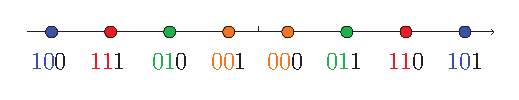
\includegraphics[width=0.5\linewidth]{figures/Set_Partition_Rule_2.eps}}
   \\
  \subfloat[]{%
  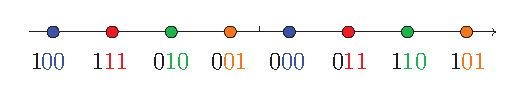
\includegraphics[width=0.5\linewidth]{figures/set_partitioning_coset_perspective.eps}}
        \hfill
\caption{Labeling of 8-AM channel signals from (a) magnitude perspective and (b) coset perspective.   The least significant two bits identify the coset. The most significant two bits indicate the magnitude.  The exclusive-or of all three bits indicates the sign.} \label{fig: 8-AM-set-partition}
\end{figure}

\subsubsection{Mapping Rule}
In order to maximize free Euclidean distance (ED) of TCM, Ungerboeck in \cite{ungerboeck1982channel} proposed a mapping rule called "mapping by set partitioning". 
Ungerboeck's set partitioning mapping rule follows from the successive partitioning of a channel-signal set into subsets with increasing minimum distance between the signals in these subsets.  With set partitioning, the coded bits serve as coset labels so that "uncoded errors" are guaranteed to have at least minimum distance between elements in the same coset.

Our design has an additional requirement that the systematic bits identify the magnitude of the symbol as produced by the distribution matcher.
Fig. \ref{fig: 8-AM-set-partition} gives binary labels for the equidistant 8-AM constellation set using a labeling that achieves both of these objectives.  In this labeling, the sign is negative when the exclusive-or of all three bits is one. The two most significant bits are the systematic bits that identify the magnitude, and one may view the least significant bit as selecting the sign.  The two least significant bits identify the coset, and one may view the most significant bit as selecting the sign. 

\subsection{Decoding Algorithms}
The channel observation at the receiver over an AWGN channel is  $\mathbf{y}=\chaninsy+\mathbf{z}$, where $\mathbf{z}\sim\mathcal{N}(\mathbf{0},\sigma^2\mathbf{I})$ is the noise vector and $\sigma^2$ is the noise variance. This subsection introduces various decoding algorithms with varied complexity and error correction performance.
We first give the definition of the codeword of a CRC-TCM-PAS system:

\begin{definition}
    $\chaninsy\in\mathcal{X}^\outlen$ is a \textit{CRC-TCM-PAS codeword} if it satisfies all of the following conditions:
    \begin{enumerate}
        \item $\chaninsy$ is a codeword of TCM.
        \item The dataword of TCM that generates $\chaninsy$, $\crcoutb$, passes the CRC check.
        \item The information bits $\crcinb$ of the CRC codeword $\crcoutb$, are the binary representation of a codeword in $\mathcal{C_{\mathrm{DM}}}$.
    \end{enumerate}
\end{definition}
Denote the codebook of CRC-TCM-PAS by $\mathcal{C}_{\mathrm{CTP}}$, which has cardinality $|\mathcal{C}_{\mathrm{CTP}}|=2^\numbits$. 
\subsubsection{Maximum Likelihood (ML) Decoder}  For AWGN, the ML decoder finds $\hat{\chaninsy}\in\mathcal{C}_{\mathrm{CTP}}$ that has smallest Euclidean distance with $\mathbf{y}$, i.e.:
\begin{align}\label{equ: MLD}
    \hat{\chaninsy}=\argminB_{\chaninsy\in\mathcal{C}_{\mathrm{CTP}}}||\chaninsy-\mathbf{y}||_2^2.
\end{align}
The ML decoder minimizes the FER, i.e., the probability of a codeword error, in AWGN.  The decoding rule of \eqref{equ: MLD} can be realized by serial list Viterbi decoding (SLVD)\cite{seshadri1994list}.
SLVD first finds the most likely path in tail-biting trellis $\mathcal{T}$. If the
constellation point sequence corresponding to this path is not a codeword in $\mathcal{C}_{CTP}$, then SLVD is used again to find the next most likely path. If a path belongs to the sub-trellis $\mathcal{T}_i$, the  trellis-tree algorithm (TTA) \cite{soong1990fast} for $\mathcal{T}_i$ is used for tracing back that path.


The ML decoding complexity can be decomposed into two parts. First, the initialization step calculates the metrics of local best paths in each of $2^\nu$ sub-trellises. Second, if a path in $\mathcal{T}_i$ needs to be traced back, a data set of TTA for 
 $\mathcal{T}_i$ needs to be constructed and maintained \cite{soong1990fast}.

 \subsubsection{$\beta$-States Decoder}  
 One solution to reduce the complexity of ML decoder is to consider only a subset of $2^\nu$ states as the possible start/end states. We denote the subset by $\Tilde{\mathcal{V}}\subseteq\mathcal{V}$ and the cardinality of  $\Tilde{\mathcal{V}}$ by $|\tilde{\mathcal{V}}|$. In this paper, we refer to a $\beta$-States decoder as a decoder that considers $\beta$ states as start/end states, i.e., $|\Tilde{\mathcal{V}}|=\beta$. Let $v(\chaninsy)$ be the TBCC initial state of  the codeword $\chaninsy$.  The $\beta$-States decoder solves the following problem:
\begin{align}\label{equ: bSD}
    \hat{\chaninsy}=\argminB_{\substack{{\chaninsy}\in\mathcal{C}_{\mathrm{CTP}}\\v(\chaninsy)\in\Tilde{\mathcal{V}}} }||\chaninsy-\mathbf{y}||_2^2.
\end{align}
The set $\Tilde{\mathcal{V}}$ is identified using one iteration of the wrap-around Viterbi algorithm (WAVA)\cite{rosewava}. 

\begin{figure*}[t] 
    \centering
      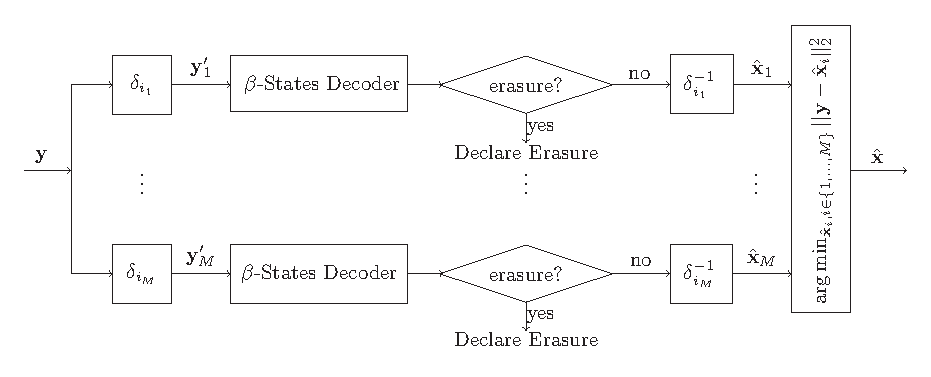
\includegraphics[width=1\linewidth]{figures/AED_structure_2.eps}
      \caption{The diagram of an AE decoder with $M$ parallel $\beta$-States decoders, i.e., AED($M$,$\beta$). }
      \label{fig: AED_str}
\end{figure*}

\subsubsection{Automorphism Ensemble (AE) Decoder}
Ensemble decoding algorithms \cite{geiselhart2022automorphism} employ $M$ parallel independent and identical sub-optimal decoders, with each proposing a codeword estimate.  From among these $M$ proposed codewords, the ensemble decoder selects the most likely candidate as the decoder output \cite{geiselhart2022automorphism}. One category of ensemble decoding utilizes automorphism groups. An automorphism group is a set of permutations such that the permuted sequence of any codeword is still a codeword.  When an automorphism group of the codes is known, identical constituent decoders decoding permuted versions of the channel output may be used, yielding the so-called Automorphism Ensemble (AE) decoding \cite{geiselhart2022automorphism}. 
 
The cyclic shifts $\delta_i$, $i=0,...,\outlen-1$, are elements of an automorphism group of the TBCC, where  $\delta_i$ indicates the cyclic shift of a sequence by $i$ positions. Hence, as illustrated in Fig. \ref{fig: AED_str}, an AE decoder for the CRC-TCM-PAS system is constructed by employing $M$ parallel $\beta$-States decoders for the channel observations that are cyclic-shifted by  $\{\delta_{i_1},\ldots,\delta_{i_M}\}$. The $i^{th}$ $\beta$-States decoder either provides a shifted estimation candidate or declares an erasure. The final decoding result of the AE decoder is the candidate that has the smallest Euclidean distance from the channel observation. We denote an AE decoder with M parallel decoders with cyclic  shifts $\{{i_1},\ldots,{i_M}\}$, where each decoder utilizes $\beta$ starting states obtained by WAVA as the decoder AED($M$, $\beta$). In this paper, the cyclic shifts  $\{{i_1},\ldots,{i_M}\}$ are uniformly sampled from $\{0,\ldots,\outlen-1\}$. 

The $M$ independent $\beta$-States decoders of AED($M$, $\beta$) can be run in parallel, so the AED($M$, $\beta$) has the same time complexity with a single $\beta$-States decoder but provides  more potential codewords. However, the AED($M$, $\beta$) requires more hardware resources than a single $\beta$-States decoder.

\section{Channel Input Distribution of CRC-TCM-PAS System }\label{sec: property}
This section proves that the distribution of the channel input $X$ of the CRC-TCM-PAS system is symmetric, i.e., $P_X(x)=P_X(-x)$ for $x\in\mathcal{X}$, where $\mathcal{X}$ is the PAM constellation set. We begin the proof with a theorem that shows the CRC check bits in the CRC-TCM-PAS system are asymptotically uniform, even though the input bits of the CRC encoder are not.

\subsection{Uniformity of CRC bits}
Denote the random variable that represents a DM output symbol by $\bar{A}$ with PMF  $P(\bar{A})$. Because the cardinality of output symbol set is $2^{k_0}$, $\bar{A}$ can be represented by $k_0$ bits, which are denoted by $B_i$, $i=0,\ldots,\ccinnum-1$.
Since $\bar{A}$ is not uniform,  $B_i$, $i=0,\ldots,\ccinnum-1$, may have different distributions. Let $a\in\mathcal{A}$ be a realization of $\bar{A}$, and  let $\mathbf{b}(a)=[b_{k_0-1}(a),\dots, b_{1}(a),~b_{0}(a)]\in\mathbb{F}_2^{k_0}$ be the binary representation of $a$.  The PMF of $B_i$ is calculated by:
\begin{align}\label{equ: distribution}
    P_{B_i}(b)=\sum_{a=0}^{|\mathcal{A}|-1}P_{{\bar{A}}}(a)\mathbbm{1}\left(b_i(a)=b\right),
\end{align}

$b=0,1,~i=0,1,...,k_0-1$. $\mathbbm{1}(\cdot)$ is the indicator function. As shown in Fig. \ref{fig: transmitter}, the binary converter maps a length-$\length$ symbol sequence to a length-$\ccinnum\length$ binary sequence.  Let $G^{\ccinnum\length}=[G_0,\ldots,G_{\ccinnum \length -1}]$ be the random vector representing the binary sequence. Assume that the DM generates i.i.d. symbols, the $G_i$'s that correspond to the same symbol bit position have the same distribution, i.e.:
\begin{align}\label{equ: prob_gi}
    P(G_i)=P(B_{i\pmod{\ccinnum}} )~,i=0,\ldots,\ccinnum\length-1.
\end{align}
Let $\mathbf{g}\in\mathbb{F}_2^{\ccinnum\length}$ be a realization of $G^{\ccinnum\length}$, and denote the polynomial form of $\crcinb$ by $g(x)=\sum_{i=0}^{k_0\length-1}g_ix^i$.

An $m$-bit CRC is specified by a degree-$m$ binary polynomial $p(x)=\sum_{i=0}^mp_{i}x^i$. 
Let the polynomial form of the output of the CRC encoder be $h(x)=\sum_{i=0}^{k_0\length+m-1}h_ix^i$. $h(x)$ is calculated by
\begin{align}\label{equ: CRC_encoding}
    h(x)=x^mg(x)+x^m g(x)\pmod{p(x)}.
\end{align}


The following theorem proves that the CRC check bits, $h_i$, $i=0,\ldots,m-1$, can be arbitrarily close to be  equally likely, with a proper choice of $l$.

\begin{theorem}\label{the: uniform_bits}
    For a length-$\length$ random vector $A^\length$ whose elements $A_i$, $i=0,\dots,\length-1$, are i.i.d. random variables with alphabet $|\mathcal{A}|=\{0,1,2,\dots,2^{k_0}-1 \}$ and distribution $P(A)$. Let $G^{k_0 \length}$ be the binary representation of $A^\length$ and $H^{k_0\length+m}$ be the CRC output sequence by encoding $G^{k_0\length}$  with some degree-m CRC polynomial $p(x)$. For any $0<\epsilon<0.5$, there exists an $l$ such that
    \begin{align*}
        |P_{H_i}(0)-0.5|<\epsilon,~i=0,1,\dots,m-1.
    \end{align*}
\end{theorem}

\begin{proof}
Define the set of random variables in $G^{\ccinnum \length}$ that belong to the $j^{th}$ symbol bit position by $\mathcal{G}_j$, i.e.,
$\mathcal{G}_j=\{G_{\ccinnum i+j},i=0,\ldots,\length-1\}$,
$j=0,\dots,\ccinnum-1$. Based on \eqref{equ: prob_gi}, the random variables in the same set have same distribution. Let $P_{G_i}(0)=p_j$, if $G_i\in\mathcal{G}_j$.


A CRC code is a linear block code. Let $\mathcal{I}_i$,  $i=0,\dots,m-1$,  be the set of information bits that are constrained by $i^{th}$ parity check.
Let $J_{i,j}$ be the number of the elements belonged to both $\mathcal{I}_i$ and $\mathcal{G}_j$, i.e., $J_{i,j}=\left|\mathcal{I}_i\bigcap \mathcal{G}_j \right|$, where $i=0,\dots m-1$ and $j=0,\dots, k_0-1$. The PMF of $i^{th}$ parity check bit, $P(H_i)$,  can be calculated by:
$P(H_i)=\circledast_{G_j\in\mathcal{G}_i}P(G_j)$, where $\circledast$ denotes circular convolution.
Using the discrete Fourier transform, $P_{H_i}(0) = \frac{1}{2}+\frac{1}{2}\prod_{j=0}^{\ccinnum -1}(1-2p_j)^{J_{i,j}}$.
$P_{H_i}(0)$ is calculated by:
\begin{align}
     P_{H_i}(0) &= \frac{1}{2}+\prod_{j=0}^{\ccinnum -1}(1-2p_j)^{J_{i,j}}.
\end{align}
Because $|1-2p_j|<1$, and $J_{i,j}$ gets larger with the increase of $l$, there exists an $l$ such that for $i=0,...,m-1$, $\left|\prod_{j=0}^{\alpha-1}(1-2p_j)^{J_{i,j}}\right|<\epsilon$.
\end{proof}

Note that Theorem \ref{the: uniform_bits} can be generalized to any systematic linear block code, and it validates the uniform check bit assumption in \cite{pas_bocherer_1}.

\begin{example}
    Let P(A)=(0.072,0.165,0.321,0.442).  For a degree-5 CRC with $p(x)=x^5+x^4+x^2+1$, the minimum $l$ that gives $|P_{H_i}(0)-0.5|<10^{-4},~i=0,\dots,4,$ is 20. 
\end{example}
\begin{remark}
Theorem \ref{the: uniform_bits} can be generalized to any systematic linear block code, and it validates the uniform check bit assumption in \cite{pas_bocherer_1}. 
\end{remark}

\subsection{Symmetry of Channel Input Distribution}
Consider a length-$\outlen$, rate-$\frac{\ccinnum}{\ccinnum+1}$, systematic, and recursive TBCC with $\nu$ memory elements.
Denote the input symbol in stage $t$ by $u_t\in\mathcal{U}$, $t=0,...,\outlen-1$ , and denote the state at time instant $t$ by $v_t\in\mathcal{V}$, $t=0,\ldots,\outlen$.
Let $\mathbf{u}_t\in\mathbb{F}_2^{k_0\times1}$ and $\mathbf{v}_t\in\mathbb{F}_2^{\nu\times 1}$ be the binary representation of $u_t$ and $v_t$, respectively.
Based on the state-space representation of convolutional code\cite{weiss2001code,fragouli1999convolutional}, $\mathbf{v}_{t+1}$ is a function of $\mathbf{v_t}$ and  $\mathbf{u_t}$, i.e., $\mathbf{v}_{t+1}=\mathbf{A}\mathbf{v}_t+\mathbf{B}\mathbf{u}_t$, where $\mathbf{A}\in\mathbb{F}_2^{\nu\times\nu}$ and $\mathbf{B}\in\mathbb{F}_2^{\nu\times k_0}$. 
The initial state $\mathbf{v}_0$ of a recursive TBCC codeword can be determined by the following equation:
\begin{align}\label{equ: initial_state}
    \mathbf{v}_0=(\mathbf{A}^{\outlen}+\mathbf{I}_\nu)^{-1}\mathbf{v}_\outlen^{[zs]},
\end{align}
where $\mathbf{I}_\nu$ is a size $\nu$ identity matrix and $\mathbf{A}^\outlen+\mathbf{I}_{\nu}$ is an invertible matrix\cite{weiss2001code}. The term $\mathbf{{v}}_N^{[zs]}$ is referred to as zero-state solution and is the final state by encoding the dataword with initial state ${0}$.  The encoding of tail-biting convolutional code has two steps: 

\begin{enumerate}
    \item Run encoding process first time by setting $v_0=0$ and record ${{v}}_\outlen^{[zs]}$.
    \item Run encoding process second time by setting ${v}_0$ using \eqref{equ: initial_state} and generate output symbols.
\end{enumerate}

Therefore, in order to study the distribution of the output symbols of a recursive TBCC, we need to know the distribution of ${{v}}_\outlen^{[zs]}$ by analyzing the first encoding process. 

For the CRC-TCM-PAS system, the data frames, i.e., input symbols,  of TBCC are the outputs of CRC encoder. Because the CRC encoder is systematic, the first $n-\frac{m}{k_0}$ input symbols of TBCC have DM output symbol distribution $P(\bar{A})$. Based on Theorem \ref{the: uniform_bits}, the last $\frac{m}{k_0}$ input symbols have uniform distributions. This subsection uses state-space representation of convolution code in \cite{weiss2001code,fragouli1999convolutional} to analyze the PMF of the state in time instant $t$, $V_t$. The PMF of $V_t$, is calculated by:
\begin{align}
    P_{V_t}(v_t)
    =\sum_{v_{t-1}\in\mathcal{V}}P(v_{t-1})\sum_{(v_{t-1},\ccoutputrealize_t},v_t)\in\mathcal{E} P(\ccoutputrealize_t,v_{t}|v_{t-1}).\label{equ: state_equ}
\end{align}
Let $ {u}_t= g^{-1}\left(v_{t-1},\ccoutputrealize_t,v_t\right)\in \mathcal{U}$ be the input symbol that associates to the edge $(v_{t-1},\ccoutputrealize_t,v_t)$.
Hence, $P(\ccoutputrealize_t,v_t|v_{t-1})=P_{U_t}\left(g^{-1}\left(v_{t-1},\ccoutputrealize_t,v_t\right)\right)$. If the convolution code is systematic, the input corresponded to $(v_{t-1},\ccoutputrealize_t,v_t)$ can be solely determined by $\\ccoutputrealize_t$, we use $g^{-1}(\ccoutputrealize_t)=g^{-1}\left(v_{t-1},\ccoutputrealize_t,v_t\right)$ as a simplification.
Define the matrix $\mathbf{C}_{t-1}\in\mathbb{R}^{|\mathcal{V}|\times|\mathcal{V}|}$ as follows:
\begin{align}\label{equ: sto_mat}
    \mathbf{C}_{t-1}(v_{t},v_{t-1})=P(v_t|v_{t-1})=\sum_{(v_{t-1},\ccoutputrealize_t,v_t)\in\mathcal{E}} P(\ccoutputrealize_t,v_{t}|v_{t-1}).
\end{align}
Let $\mathbf{p_t}=\left[P_{V_t}(0)\dots P_{V_t}(2^{\nu}-1)\right]^T$, \eqref{equ: state_equ} can be rewritten as:
\begin{align}\label{equ: state_pmf}
    \mathbf{p}_t=\mathbf{C}_{t-1}\mathbf{p}_{t-1}= \left(\prod_{i=0}^{t-1} \mathbf{C}_{i}\right)\mathbf{p}_0, ~t=1,2,...,\outlen.
\end{align}

\eqref{equ: sto_mat} implies that $\mathbf{C}_{t-1}$ is a left stochastic matrix, i.e., each column in $\mathbf{C}_{t-1}$ is a probability vector. Moreover, $\mathbf{C}_{t-1}$ is also right stochastic, meaning that each row has a sum of 1. To see this, for the trellis of a convolutional code, for each $v_{t}\in\mathcal{V}$, there are $2^{k_0}$ edges that connect $v_t$ and each edge associates a distinct input in $\mathcal{U}$. As a result, $\mathbf{C}_{t-1}$ is a doubly stochastic matrix.

\begin{theorem}\label{the: uinform_state}
    For an $(\ccoutnum,\ccinnum,\nu)$ convolutional code with any initial state distribution $P(V_0)$, if the data frames are i.i.d. random variables with PMF $P(U)$ and $P_U(u)>0$ for any $u\in\mathcal{U}$. Let $V_t$ be the state at time instant $t$, then the random sequence $V_0,V_1,\ldots$ converges in distribution to a uniform random variable ${V}_{\mathrm{uni}}$, i.e., $V_t\xrightarrow{d}{V}_{\mathrm{uni}}$.
\end{theorem}

\begin{proof}
    Because all the data frames have the same distribution, it has $\mathbf{C}_t=\mathbf{C}$. Hence, \eqref{equ: state_pmf} can be rewritten as
    %\begin{align}\label{equ: state_pmf_2}
    $\mathbf{p}_{t}=\mathbf{C}^{t}\mathbf{p}_0$.
    %\end{align}
    $\mathbf{C}$ is not only a doubly stochastic matrix but also a regular matrix.
    For a convolutional code, any state $v_i \in \mathcal{V}$ can always reach any state $v_j\in\mathcal{V}$ with a finite-length path. $\mathbf{C}$ retains this property, because $P_U(u)>0$, for any $u\in\mathcal{U}$.
    As a result, $\mathbf{C}$ is regular.
    Based on Perron-Frobenius theorem\cite{gantmakher2000theory}, the non-negative and regular matrix $\mathbf{C}$ has the following properties:
    \begin{enumerate}
        \item  $\mathbf{C}$ has $\lambda_1=1$  as an eigenvalue of multiplicity 1, and the normalized right eigenvector corresponded to eigenvalue 1 is $\mathbf{q}^*=\left[\frac{1}{\sqrt{2^\nu}}~\frac{1}{\sqrt{2^\nu}}\ldots\frac{1}{\sqrt{2^\nu}}\right]^{T}$.
        \item For all other eigenvalues $\lambda_j$, $j=2,...,q$, it has $|\lambda_j|$ is \emph{strictly} smaller than 1,  i.e., $|\lambda_j|<1$.
    \end{enumerate}

    Let $\mathbf{J}=\mathbf{Q}^{-1}\mathbf{C}\mathbf{Q}$ be the  Jordan canonical form   of $\mathbf{C}$. Based on Perron-Frobenius theorem,
    $\mathbf{J}=\text{diag}(1,\mathbf{J}_2,\dots,\mathbf{J}_q),$
    where $\mathbf{J}_2,\ldots,\mathbf{J}_q$ are Jordan block matrices that correspond to eigenvalues $\lambda_2,\ldots$,$\lambda_q$, respectively.
    Let $\mathbf{Q}=[\mathbf{q}_1\dots\mathbf{q}_{2^\nu}]$ and, $\mathbf{q}_1$ is the eigenvector associated to eigenvalue 1, $\mathbf{q}_1= \alpha\mathbf{q}_1^*$, $\alpha\in\mathbb{R}$.
    Let $\mathbf{p}_0=\sum_{i=1}^{2^\nu}c_i\mathbf{q}_i=\mathbf{Q}\mathbf{c}$, it has $\mathbf{p}_t=\mathbf{C}^t\mathbf{p}_0=\mathbf{Q}\mathbf{J}^t\mathbf{c}$.
    Because
    $\lim_{t\rightarrow \infty}\mathbf{J}_i=\mathbf{0}$ for $j=2,\ldots, 2^{\nu}$, it has $\lim_{t\rightarrow \infty} \mathbf{p}_t = c_1\alpha\mathbf{q}_1^* =\left[\frac{1}{2^\nu}\dots \frac{1}{2^\nu}\right]^T$.
    % \begin{align}
    %     \lim_{t\rightarrow \infty} \mathbf{p}_t &= c_1\alpha\mathbf{q}_1^* =\left[\frac{1}{2^\nu}\dots \frac{1}{2^\nu}\right]^T\label{equ: final_uniform}.
    % \end{align}
    %\eqref{equ: final_uniform} follows the fact that $\mathbf{p}_N$ is a valid distribution.
    %Thus, when $\outlen$ is large enough, $P(V_\outlen)$ converges to uniform distribution.
\end{proof}

\begin{example}
    Consider the (3,2,3) convolution code shown in Fig. \ref{fig: transmitter}. Let the initial state be 0 and $P(U)=(0.5742,0.3188, 0.01642,0.09048)$.  When $t=12$, $|P_{V_{12}}(v)-\frac{1}{8}|<10^{-4}$, $v=0,\ldots,7$.
\end{example}

Besides, if the state distribution at time $t$ is  uniform, the state distribution at time $t+1$ is also uniform, no matter what $P(U_t)$ is. Hence, the zero-state solution, as well as the initial state of TBCC,  have a uniform distribution.
As indicated in \eqref{equ: initial_state}, the TBCC initial state is a one-to-one mapping of zero-state solution, thus the initial state of TBCC  has uniform distribution. 
As a result, the states at all $\outlen+1$ time instants in second encoding process have uniform distribution.


Now, we show that if the state at time instant $t$ is uniform, then the ($k_0+1,k_0,\nu$) systematic recursive TBCC generates an equally likely parity check bit in stage $t$. First of all, the following theorem gives that distribution of output symbol in stage $t$.


\begin{theorem}\label{the: sym_dist}
Consider a $(k_0+1,k_0,\nu)$ systematic recursive  convolutional code that is defined by state set $\mathcal{V}$, edge set $\mathcal{E}$, input set $\mathcal{U}$, and output set $\ccoutputset$. If the state distribution at time instant $t$ is uniform, i.e., $\mathbf{p}_t=\left[\frac{1}{2^\nu}\frac{1}{2^\nu}\dots \frac{1}{2^\nu}\right]^T$, then the output symbol distribution in stage $t$, $P_{O_t}(\ccoutputrealize_t)=\frac{1}{2} P_{U_t}\left(g^{-1}(\ccoutputrealize_t)\right)$, $\forall \ccoutputrealize_t\in\ccoutputset$.
\end{theorem}

\begin{proof}
Define matrix $\mathbf{D}_t\in\mathbb{R}^{|\ccoutputset|\times|\mathcal{V}|}$ with $\mathbf{D}_t(\ccoutputrealize_t,v_{t-1})=P(\ccoutputrealize_t|v_{t-1})$, where $\ccoutputrealize_t\in\ccoutputset$ and $v_{t-1}\in\mathcal{V}$. Define $\mathbf{q}_{t}=[P_{O_t}(0) \dots P_{O_t}(|\ccoutputset|-1)]^T$. $\mathbf{q}_{t}$ can be calculated by $\mathbf{q}_t=\mathbf{D}_{t-1}\mathbf{p}_t$.

Because the TBCC is systematic, $\mathbf{D}_t(\ccoutputrealize_t,v_{t-1})=P_{U_t}(g^{-1}(\ccoutputrealize_t))$.  Hence, one property of $\mathbf{D}_t$ is that the non-zero elements in each row have the same value.

The other property  is that $\mathbf{D}_t$ contains $2^{\nu-1}$ non-zero elements for each row, 
i.e., given any output $\ccoutputrealize_t\in\ccoutputset$, there are only $2^{\nu-1}$ possible states from which $\ccoutputrealize_t$ can be generated. This is because for a rate-$\frac{\ccinnum}{\ccinnum+1}$, systematic, recursive convolution code, the register adjacent to the output is determined by $\ccoutputrealize_t$,  hence the freedom of $v_{t-1}$ is reduced by 1. Based on the two properties of $\mathbf{D}$, for any $\ccoutputrealize_t\in\ccoutputset$,  it has: $P_{O_t}(\ccoutputrealize_t) = \sum_{i=1}^{2^\nu}\mathbf{D}(l,i)P_{V_t}(i)=\frac{1}{2}P_{U_t}(g^{-1}(\ccoutputrealize_t))$.
\end{proof}

Theorem \ref{the: sym_dist} implies that, if the state distribution at time $t$ is uniform, then the parity bit generated by the convolutional code at stage $t$ is uniform. Because the sign value of the channel input symbol at stage $t$, $X_t$, is determined by parity bit, it has $P_{X_t}(x)=P_{X_t}(-x)$, for $x\in\mathcal{X}$.
Note that one rule of channel-signal mapping function in CRC-TCM-PAS is that information bits indicate magnitude and parity check bit indicates sign.


Because the states of each time instant of TBCC have uniform distribution, the channel inputs in each stage have symmetric distributions. Besides, the magnitude distributions of first $\outlen-\frac{m}{k_0}$ and last $\frac{m}{k_0}$ channel inputs follow $P(\bar{A})$ and uniform distribution, respectively.

\section{FER Upper Bound for CRC-TCM-PAS System}\label{sec:tfbound}
In this section, we derive the  FER upper bound for the CRC-TCM-PAS system with the specified CC, CRC, and an ideal distribution matcher that generates length-$l$ symbol sequences with the desired distribution $P(\hat{A}^ \length)$. 
The upper bound is computed using the generating function of an equivalent convolutional code whose error events correspond exactly
to the undetectable error events of the concatenation of the original CRC and CC. 

\subsection{Equivalent Code for CRC-Aided Convolutional Code}\label{sec: equ_code}
As shown in Fig. \ref{fig: transmitter}, the binary representation  of the symbol sequence generated by a  distribution matcher is encoded by a CRC and a TBCC serially. We begin our analysis by replacing the CRC and convolutional encoder with a single convolutional encoder whose input is the quotient of dividing the CRC codeword by the CRC polynomial.

Let $\mathbf{h}$ be a length-$(\equl+m)$ CRC codeword with polynomial form $h(x)=\sum_{t=0}^{\equl+m+1} h_tx^{t}$. Based on the notation in Fig. \ref{fig: transmitter}, $\equl=\ccinnum\length$. For a rate-$\frac{\ccinnum}{\ccinnum+1}$ convolutional code, there are $\ccinnum$ input branches. Let the input of the $i^{th}$ branch be $\mathbf{h}^{(i)}$, and let the corresponding polynomial be $h^{(i)}(x)$. $\mathbf{h}^{(i)}=[h_i~h_{\ccinnum i}\ldots h_{\equl+m-\ccinnum+i}]$ is obtained by sampling $\mathbf{h}$ every $\ccinnum$ positions starting from $i^{th}$ position, and $h^{(i)}(x)=\sum_{t=0}^{(\equl+m)/\ccinnum -1}{h}_{\ccinnum t+i}x^{t}$, $i=0,\ldots,k_0-1.$ 

 

Let $\crcquot$ be the quotient of dividing the CRC output by the CRC polynomial. The polynomial form of $\mathbf{q}$, $q(x)$, is calculated by 
\begin{equation}\label{equ: quotient}
  \crcquotel(x):= h(x)/p(x).
\end{equation}


\begin{theorem}
    Consider an $m$-bit CRC encoder which is specified by an $m$-degree polynomial $p(x)$. Let the number of input bits be $\equl$. Let $\ccinnum$ be an integer that divides $m+\equl$. Then for any codeword polynomial $h(x)$, its $\ccinnum$-split polynomial vector, $\mathbf{h}_{\ccinnum}(x)$ can be calculated by $\mathbf{h}_{\ccinnum}(x) = \mathbf{q}_{\ccinnum}(x) \peq(x)$.
    \begin{align}
        \mathbf{h}_{\ccinnum}(x) = \mathbf{q}_{\ccinnum}(x) \peq(x),
    \end{align}
    where $\mathbf{q}_{\ccinnum}(x)$ is the $\ccinnum$-split polynomial vector of $q(x)=h(x)/p(x)$  and $\mathbf{P}_{\mathrm{eq}}(x)\in\mathbb{F}_2[x]^{k_0\times k_0}$ is a $k_0\times k_0$ square binary polynomial matrix.
\end{theorem}

\begin{proof}
Based on the relationship $h(x)=p(x)q(x)$, the $t^{th}$ bit of $\mathbf{h}^{j}$, $h^{(j)}_t$ is calculated by:
\begin{align}
    h_t^{(j)}
    &= h_{k_0t+j} = \sum_{s=0}^m q_{k_0t+j-s}p_s\\
    &= q_{k_0t+j}p_0+ \sum_{\ell = 0}^{ m/k_0  - 1} \sum_{s'=1}^{k_0} q_{k_0t+j-k_0\ell-s'} p_{k_0\ell+s'}\\
    &= \sum_{\ell = 0}^{ m/k_0  - 1} \sum_{i=0}^j q_{k_0(t-\ell)+i} p_{k_0\ell+j-i}+\sum_{\ell = 1}^{ m/k_0}\sum_{i=j+1}^{k_0-1} q_{k_0(t-\ell)+i} p_{k_0\ell+j-i}+q_{k_0t+j-m}p_m
\end{align}
Let $p^{(i)}_t = p_{kt+i}$, $h^{(j)}_t$ can be rewritten as:
\begin{align}
    h_t^{(j)} &= \sum_{i=0}^j \sum_{\ell = 0}^{ m/k_0  - \mathbbm{1}(i\neq j)} \crcquotel^{(i)}_{t-\ell} p^{(j-i)}_{\ell} \nonumber \\&+ \sum_{i=j+1}^{k_0-1} \sum_{\ell = 0}^{ m/k_0  - 1} \crcquotel^{(i)}_{t-\ell-1} p^{(j-i+k_0)}_{\ell+1}.
\end{align}
Define $p^{(i)}(x)=\sum_{t=0}^{m/\ccinnum-\mathbbm{1}(i=0)}p_{\ccinnum t+i}x^{t}$. The $h^{(j)}(x)$ can be calculated by: 
% \begin{align}
% p^{(i)}(x) = 
%     \begin{cases}
%       \sum_{t=0}^{m/{\ccinnum}-1} p_{\ccinnum t+i}x^{t}, & i\neq 0\\
%      \sum_{t=0}^{m/\ccinnum} p_{\ccinnum t}x^{t}, & i=0.
%     \end{cases}
% \end{align}
% we have
\begin{align}\label{equ: uj_x}
    h^{(j)}(x) =& \sum_{i=0}^j \crcquotel^{(i)}(x)p^{(j-i)}(x)+ \sum_{i=j+1}^{\ccinnum  -1} x\crcquotel^{(i)}(x) p^{(j-i+\ccinnum)}(x)\,.
\end{align}
\eqref{equ: uj_x} implies that, by choosing the polynomial of $i^{th}$ row and $j^{th}$ column of $\peq(x)$ as:
\begin{align}\label{equ: peq2}
\peq(x)_{i,j} = p^{(j-i)}(x)\mathbbm{1}(i\leq j)+xp^{(j-i+\ccinnum)}(x)\mathbbm{1}(i > j),
    % \begin{cases}
    %   p^{(j-i)}(x) & i\leq j \\
    %  xp^{(j-i+\ccinnum)}(x) & i > j 
    % \end{cases},
\end{align}
it has 
\begin{align}
\mathbf{h}_{\mathrm{split}}(x) = \crcquotsplit \peq(x).
\end{align}
\end{proof}
As a result, the concatenation of a CRC with generator polynomial $p(x)$ and a rate-$\frac{\ccinnum}{\ccinnum+1}$ convolutional code with generator matrix $\convc(x)$ is equivalent to a  convolutional code with generator matrix $\ceq(x)$, which is defined as follows:
\begin{equation}\label{eq:ceqdef}
\ceq(x) = \peq(x) \convc(x).
\end{equation}
The error events of the equivalent convolutional code correspond exactly to the error events of the original concatenation of CRC and convolutional code.
Because the concatenation of a CRC expurgates the original TBCC by removing the codewords whose corresponding messages do not pass the CRC, the remaining codewords all meet the tail-biting condition so that the equivalent convolutional code is still tail-biting. 

\subsection{FER Upper Bound} \label{subsec: fer_upperbound}
This subsection bounds the FER for the CRC-TCM-PAS system. Based on the analysis in the previous subsection, the CRC-aided TBCC can be replaced by an equivalent TBCC with the generator matrix given in $\eqref{eq:ceqdef}$. The final computation of FER requires the output symbol distributions.  For the purposes of this analysis, we assume a  distribution matcher that generates $\length$ i.i.d. symbols with the target symbol distribution $P(A)$.  After the distribution matcher, $n-\length$ CRC symbols are appended to the sequence.  Based on Theorem \ref{the: uniform_bits}, these CRC symbols should be approximated as having a uniform distribution rather than $P(A)$.  
The output symbol distributions for the analyzed system of the equivalent TBCC with the generator matrix given in $\eqref{eq:ceqdef}$ with our idealized distribution matcher are thus $\length$ output symbols distributed according to $P(A)$ and $n-\length$ output symbols distributed according to a uniform distribution. 
%Let the codeword length be $\outlen$, the magnitude distributions of first $\length$ and last $n-\length$ output symbols are $P(A)$ and uniform distribution, respectively.} 

Let $\mathcal{C}_{\mathrm{T}}\subset\mathcal{X}^{\outlen}$ be the codebook of TCM. 
%Let $\mathbf{u}\in\mathcal{A}^{\outlen}$ be the input symbol sequence of TBCC. 
Let $\mathbf{x}_c\in\mathcal{C}_{\mathrm{T}}$ be the transmitted codeword, and let $\mathbf{y}$ be the channel observation over AWGN channel. Let $\errorevent$ denote the event that, given observation $\mathbf{y}$, an ML decoder selects  $\hat{\x} \neq \xc$. Let $\PEE$ denote the event that, given $\y$,  codeword $\xe$ is more likely than codeword $\xc$. The FER of CRC-TCM-PAS transmission system $P_e$  is upper bounded by the union bound:
\begin{align}
    P_e&=\sum_{\mathbf{x}_c\in\mathcal{C}_{\mathrm{CT}}}P(X^\outlen=\mathbf{x})P\left(\errorevent\right)\\
    &=\sum_{\mathbf{x}_c\in\mathcal{C}_{\mathrm{CT}}}P(X^\outlen=\mathbf{x})P\left(\bigcup_{\substack{\mathbf{x}_e\in\mathcal{C}_{\mathrm{CT}}\\\mathbf{x}_c\neq\mathbf{x}_e}}\PEE\right)\\
    &\leq \sum_{\mathbf{x}_c\in\mathcal{C}_{\mathrm{T}}}P(X^\outlen=\mathbf{x}_c)\sum_{\substack{\mathbf{x}_e\in\mathcal{C}_{\mathrm{T}}\\\mathbf{x}_e\neq\mathbf{x}_c}}P\left(\PEE\right)\label{equ:PEPbound}.
\end{align}

The probability $\PEP$ is referred as the pairwise error probability (PEP). 
With the assumption of i.i.d. symbols of distribution matcher, and based on the analysis on CRC bits and channel inputs, 
Because the input symbols are independent, it has $P(X^\outlen=\mathbf{x})=\prod_{i=0}^{\outlen}P(X_i=x_i)$. 
Not that the distributions of $P(X_i)$, $i=0,...,\length-1$ can be derived from $P(\bar{A})$ and last $\frac{m}{k_0}$ symbols in $\mathbf{x}$ have uniform distribution.

Because $P(X^n)$ is non-uniform\footnote{In a practical CRC-TCM-PAS system, the codewords are uniform, specifically, $P_{X^n}(\mathbf{x})=\frac{1}{2^k}\mathbbm{1}(\mathbf{x}\in\mathcal{X}_{\mathrm{CTP}}).$ }, choosing the codeword that has the smallest Euclidean distance with the channel observation is no longer optimal. Let $\uc,\ue$ denote the convolutional inputs corresponding to outputs $\xc, \xe$, $\PEE$ happens if $P_{X^\outlen|Y^\outlen}\left(\xe | \y\right) > P_{X^\outlen|Y^\outlen}\left(\xc | \y\right)$, this condition is equivalent to:
\begin{align}
    &\log\left(f(\y | \xe ) P_{X^\outlen}(\xe) \right) > \log\left(f(\y | \xc)P_{X^\outlen}(\xc) \right)\label{equ: log_ineq}\\
    \iff& ||\xc-\y||_2^2 - ||\xe-\y||_2^2 > 2\noisestd^2 \log\left(\frac{P_{X^\outlen}(\xc)}{P_{X^\outlen}(\xe)}\right)\\
    %\label{equ:PEPcond0}
    \iff&2\left\langle \y - \xc, \xe - \xc \right\rangle- ||\xc-\xe||_2^2 > 2\noisestd^2 \log\left(\frac{P_{X^\outlen}(\xc)}{P_{X^\outlen}(\xe)}\right).\label{equ:PEPcond0}
\end{align}
$\langle\cdot,\cdot\rangle$ represents the inner product and $||\cdot||_2$ represents $l^2$-norm.  

Define $z'$ as follows:
\begin{align}
    \label{equ:yprimedef}
    z' = \frac{\langle \y-\xc, \xe - \xc \rangle}{||\xc - \xe ||_2},
\end{align}
it can be proved that $z'\sim\mathcal{N}(0,\sigma^2)$. Manipulating \eqref{equ:PEPcond0} reveals that $\PEE$ occurs if the following inequality is satisfied: 
\begin{align}
    \label{equ:PEPcond1}
    z' &> \frac{1}{2}||\xc - \xe ||_2 + \frac{\noisestd^2}{||\xc - \xe ||_2}\log\left(\frac{P_{X^\outlen}(\xc)}{P_{X^\outlen}(\xe)}\right) \\ &\triangleq  \frac{1}{2}\dplain(\xc, \xe).
\end{align}
Note that $\dplain$ is not a metric as $d(\xc,\xe)\neq d(\xe,\xc)$.

Applying (\ref{equ:PEPcond1}) yields
\begin{equation}
    \label{equ:PEPcond2}
    \PEP = Q\left(\frac{\sqrt{d^2\left(\xc, \xe\right)}}{2\noisestd}\right),
\end{equation}
where
\begin{align}
    \label{equ:dnewdef}
    \dplain^2(\xc, \xe) = & ||\xc - \xe ||_2^2   + 4\noisestd^2 \log\left(\frac{P_{X^\outlen}(\xc)}{P_{X^\outlen}(\xe)}\right) + \left(\frac{2\noisestd^2}{||\xc - \xe ||_2}\log\left(\frac{P_{X^\outlen}(\xc)}{P_{X^\outlen}(\xe)}\right)\right)^2.
\end{align}

Define $\da^2(\xc, \xe)$ by neglecting the last squared term in \eqref{equ:dnewdef}, i.e.:
\begin{equation}
    \label{equ:dadef}
    \da^2(\xc, \xe) = ||\xc - \xe ||_2^2 + 4\noisestd^2 \log\left(\frac{P_{X^\outlen}(\xc)}{P_{X^\outlen}(\xe)}\right).
\end{equation}
 Because $\da^2(\xc, \xe) \leq \dplain^2(\xc, \xe)$, the PEP $P(\PEE)$ is upper bounded by:
\begin{align}
    P(\PEE) = Q\left(\frac{\sqrt{\dplain^2{(\xc,\xe)}}}{2\sigma}\right) \leq Q\left(\frac{\sqrt{\da^2{(\xc,\xe)}}}{2\sigma}\right).
\end{align}

Hence, $P_e$ is further bounded by:
\begin{align}\label{equ: PEPbound2}
P_e\leq\sum_{\mathbf{x}_c\in\mathcal{C}_{\mathrm{T}}}P(X^\outlen=\mathbf{x}_c)\sum_{\substack{\mathbf{x}_e\in\mathcal{C}_{\mathrm{T}}\\\mathbf{x}_e\neq\mathbf{x}_c}} Q\left(\frac{\sqrt{\da^2{(\xc,\xe)}}}{2\sigma}\right).
\end{align}

Based on the ideal DM assumption and our analysis of CRC and TBCC encoding, the output symbols of the CRC-TCM-PAS system are independent of each other. Hence, 
\begin{align}
\da^2(\xc, \xe) = \sum_{i=1}^n\da^2\left(x_{c,i},x_{e,i}\right),
\end{align} 

where $x_{c,i}$ and $x_{e,i}$ are the $i^{th}$ element in $\mathbf{x}_c$ and $\mathbf{x}_e$, respectively, and
\begin{align}\label{equ: symbolwise_da}
    \da^2\left(x_{c,i},x_{e,i}\right)=(x_{c,i}-x_{e,i})^2+4\sigma^2\log\frac{P_{X_i}(x_{c,i})}{P_{X_i}(x_{e,i})}.
\end{align}
Besides, the omitted term
\begin{equation}
    \left(\frac{2\noisestd^2}{||\xc - \xe ||_2}\log\left(\frac{p(\uc)}{p(\ue)}\right)\right)^2\sim \left(\noisestd^2\right)^2.
\end{equation}
As a result, $\da^2$ approaches $d^2$ quadratically with SNR.

\subsection{Generating Function with State-Reduction Method}
This subsection derives the generating function of non-uniform-input TCM using Biglieri's product state method \cite{biglieri1984productstate}, with state-reduction method as described in \cite{wesel2004statereduction}. The product state diagram\cite{biglieri1984productstate} is built by replacing each state in the error state diagram with a complete encoder state diagram. Hence, for a convolutional code that has $\nu$ memory elements, there are totally $2^{2\nu}$ states in the product state diagram. Wesel in \cite{wesel2004statereduction} reduces the total number of states by proposing an "equivalence-class encoder" with $\nu_x$ memory elements.  Because $\nu_x<\nu$, the state-reduction method requires fewer states than the product state diagram. 
% , by observing that same symbol error results in the same Euclidean distance for the constellation points that belong to the same equivalent class. 
% As a result, the encoder state diagram in the product state diagram can be replaced by a equivalent class encoder diagram, resulting in $2^{\nu+\nu_x}$ states in total. Because $\nu_x<\nu$, Wesel's method delivers a diagram with less number of states.

For an equivalence-class encoder, denote the set of output by $\ccoutputset_\text{eq}$. Let $q\in\ccoutputset_\text{eq}$ be an output of the equivalent-class encoder. Let $\erro\in\ccoutputset$ be a symbol error. As a reminder, $\ccoutputset$ is the set of TBCC output symbols. Let $x_q$, $x_{q\erro}$ be any constellation point that belongs to equivalent class $q$ and the constellation point that $x_q$ moves to because of $\erro$.  We define $\da^2(q,\erro)$ as follows:
\begin{align}
    \da^2\left(q,\erro\right)=(x_{q}-x_{q\erro})^2+4\sigma^2\log\frac{P_{X}(x_{q})}{P_{X}(x_{q\erro})}.
\end{align}

We follow the notations in \cite{wesel2004statereduction} to describe the state-reduced product state diagram. Denote the set of equivalence-class encoder states and the set of error states by $\mathcal{S}_{q}$ and $\mathcal{S}_e$, respectively. 
The pair $(s_q,s_e)\in\mathcal{S}^*=\mathcal{S}_q\times\mathcal{S}_e$ describes where the states "should be" if there is no error occurs, and where the state is "drifted to" because of some error event. The notation "$\times$" means Cartesian product. Let $(\eqstart,\errstart),(\eqend,\errend)\in\mathcal{S}^*$, we label the state transition $(\eqstart, \errstart) \to (\eqend, \errend)$ with 
\begin{equation}
    \label{equ:branchlabel}
    P\left(\eqstart \to \eqend\right)
    \sum_{ \erro } \sum_{\tilde{\eq}} P\left(\tilde{\eq} | \eqstart \to \eqend\right)\, W^{\da^2(\tilde{\eq}, \erro)},
\end{equation}
where $\eqstart\rightarrow \eqend$ is the event that the state of the equivalent class encoder transits from $\eqstart$ to $\eqend$. 
The first summation is over   all possible symbol error $e_0$ due to error state diagram transition $\errstart \to \errend$, and the second summation is over   all possible equivalent class $q'$ due to equivalent-class encoder state diagram transition $\eqstart \to \eqend$.

Based on the channel-signal mapping rule, the  constellation of TCM output is symmetric with respect to 0 and the equivalence class is determined by the systematic bits.  Thus, one generator polynomial matrix of the minimal equivalent-class encoder for the rate-$\frac{k_0}{k_0+1}$, systematic TBCC in TCM is simply a size-$k_0$ identity matrix. Thus, by Theorem 1 in \cite{wesel2004statereduction},  it is sufficient to use the error state diagram to compute the transfer function, and the label of transition $\errstart \rightarrow \errend$ is $\sum_{ \erro } \sum_{\eq\in\ccoutputset_\text{eq}}P\left(\eq\right)\, W^{\da^2(\eq, \erro)}$. The equivalent class $q$ of  the constellation of TCM output is associated with the magnitude of the constellation point, which has either capacity-approaching distribution $P({A})$ for the first $n-l$ output symbols or uniform distribution for the last $l$  output symbols.
In the proposed transmission system, the magnitudes of the channel inputs are provided by either distribution matcher or CRC bits. Hence, $P(q)$ is either the empirical distribution of distribution matcher $P(\bar{A})$ or the uniform distribution $P_{\mathrm{uni}}$, depending on whether $q$ is correspond to the  distribution matcher symbols or the CRC symbols.

Define $|\mathcal{S}_e|\times|\mathcal{S}_e|$ matrices $\bigmat_A(W)$ and $\bigmat_{\text{uni}}(W)$ that enumerate all possible state transitions with equivalent-class PMFs of  $P(A)$ and uniform distribution as follows:
\begin{align}
    \bigmat_{{A}}(W)_{\errstart, \errend} = \sum_{\erro} \sum_{\eq} P_{{A}}(q) W^{\da^2(\eq, \erro)}, \\ \bigmat_{\text{uni}}(W)_{\errstart, \errend} = \sum_{\erro} \sum_{\eq} \frac{1}{|\mathcal{A}|} W^{\da^2(\eq, \erro)}.
\end{align}
We define the generating function as 
\begin{align}
\tbcc(W) = -1 +
    \sum_{i=0}^{\errcnt}
    % \mathbf{1}_{\eqcnt}
    \mathbf{e}_i
    \bigmat_A^{\length}(W)\bigmat_{\text{uni}}^{n-l}(W)
    \mathbf{e}_i^{\mathrm{T}},
\end{align} 
where $\mathbf{e}_i$ is a length $|\errcnt|$ indicator vector where ${e}_{i,j}=\mathbbm{1}(j=i)$. For the TBCC, the error events must be tail-biting paths, $\mathbf{v}_i$ selects the starting/ending state of the error events.

Define the free distance, $\dfree = \min_{\xc,\xe \in \mathcal{C}_{\mathrm{T}}} \da \left(\xc, \xe\right)$. With the inequality:

\begin{align}\label{equ: inequality}
\begin{split}
Q\left(\frac{\sqrt{\da^2{(\xc,\xe)}}}{2\sigma}\right)\leq Q\left(\frac{\sqrt{\dfree^2}}{2\sigma}\right)\exp\left(\frac{\dfree^2-\da^2{(\xc,\xe)} }{8\noisestd^2}\right),
\end{split}
\end{align}
$P_e$ in \eqref{equ: PEPbound2} is further bounded by:
\begin{align}
\begin{split}
    \label{equ:Qapprox}
    &P_e \leq Q\left(\frac{\sqrt{\dfree^2}}{2\noisestd}\right) \exp\left(\frac{\dfree^2}{8\noisestd^2}\right)\times\\&\sum_{\mathbf{x}_c\in\mathcal{C}_{\mathrm{T}}}\sum_{\substack{\mathbf{x}_e\in\mathcal{C}_{\mathrm{T}}\\\mathbf{x}_e\neq\mathbf{x}_c}}\prod_{i=1}^{\outlen} \left[\exp\left(-\frac{\da^2\left( x_{c,i}, x_{e,i} \right)}{8\noisestd^2}\right)P_{X_i}(x_{c,i})\right]\,.
\end{split}
\end{align}

Note the \eqref{equ: inequality} can be proved by $Q(\sqrt{x+y})\leq Q(\sqrt{x})e^{-\frac{y}{2}}$, for $x,y\geq 0$.
The double summation term in \eqref{equ:Qapprox} can be rewritten as follows:
\begingroup
\allowdisplaybreaks
\begin{align}
    &\sum_{\mathbf{x}_c\in\mathcal{C}_{\mathrm{T}}}\sum_{\substack{\mathbf{x}_e\in\mathcal{C}_{\mathrm{T}}\\\mathbf{x}_e\neq\mathbf{x}_c}} \left[\exp\left(-\frac{\da^2\left(\xc,\xe\right)}{8\noisestd^2}\right)P_{X^n}\left(\xc\right)\right],\\
    =& \sum_{\mathbf{x}_c\in\mathcal{C}_{\mathrm{T}}}\sum_{\substack{\mathbf{x}_e\in\mathcal{C}_{\mathrm{T}}\\\mathbf{x}_e\neq\mathbf{x}_c}} \left[W^{\da^2\left(\xc,\xe\right)} P_{X^n}\left(\xc\right)\right]\Bigr|_{W=e^{-\frac{1}{8\sigma^2}}},\\
    =& \sum_{\mathbf{x}_c,\mathbf{x}_e\in\mathcal{C}_{CT}} \left[W^{\da^2\left(\xc,\xe\right)} P_{X^n}\left(\xc\right)\right]\Bigr|_{W=e^{-\frac{1}{8\sigma^2}}}- \sum_{\mathbf{x}_c\in\mathcal{C}_{CT}} \left[W^{\da^2\left(\xc,\xc\right)} P_{X^n}\left(\xc\right)\right]\Bigr|_{W=e^{-\frac{1}{8\sigma^2}}}\\
    =& \sum_{\mathbf{x}_c,\mathbf{x}_e\in\mathcal{C}_{CT}} \left[W^{\da^2\left(\xc,\xe\right)} P_{X^n}\left(\xc\right)\right]\Bigr|_{W=e^{-\frac{1}{8\sigma^2}}}- \sum_{\mathbf{x}_c\in\mathcal{C}_{\mathrm{CT}}} \left[W^0 P_{X_i}\left(x_{c,i}\right)\right]\\
    =& \sum_{\mathbf{x}_c,\mathbf{x}_e\in\mathcal{C}_{T}} \left[W^{\da^2\left(\xc,\xe\right)} P_{X^n}\left(\xc\right)\right]\Bigr|_{W=e^{-\frac{1}{8\sigma^2}}}- 1,\\
    =&\sum_{\substack{\mathbf{q}\in\ccoutputset_\text{eq}^{\outlen}\\\mathbf{e}\in\mathcal{C}^n_{\mathrm{T}}}}\prod_{i=1}^{\outlen}\left[W^{\da^2(q_i,e_i)}P(q_i)\right]\Bigr|_{W=e^{-\frac{1}{8\sigma^2}}}-1,\\
    =& \sum_{i=0}^{|\errcnt|} \mathbf{e}_i \bigmat_A^{\length}(W)\bigmat_{\text{uni}}^{n-\length}(W) \mathbf{e}_i^{\mathrm{T}}\Bigr|_{W=e^{-\frac{1}{8\sigma^2}}}-1.
\end{align}
\endgroup
As a result, the FER upper bound can be calculated using the generating function  by
\begin{align}
    P_e \leq Q\left(\frac{\sqrt{\dfree^2}}{2\noisestd}\right) \exp\left(\frac{\dfree^2}{8\noisestd^2}\right)\tbcc\left(W=e^{-\frac{1}{{8\noisestd^2}}}\right)\,.
\end{align}

\section{Simulation results} \label{sec: simu} 


% \usepackage{multirow}
\begin{table}[t]
\caption{Optimized Convolutional Code  and CRC Pairs. All the parameters are optimized while SNR equals 11 dB.}
  \label{tab:OptimCodes}
\centering
\begin{tabular}{cc|c|c|c|c|c|}
\cline{3-7}
       &      & $H^{0}(D)$ & $H^{1}(D)$ & $H^{2}(D)$ & $p(x)$ & \begin{tabular}[c]{@{}l@{}}FER\\ bound\end{tabular} \\ \hline
\multicolumn{1}{|l|}{\multirow{2}{*}{\begin{tabular}[c]{@{}l@{}}$\nu=3$\\ $m=2$\end{tabular}}} & Ung. & 13           & 04           & 00           & 7      & 6.65e-4   \\ \cline{2-7} 
\multicolumn{1}{|l|}{}                                                                         & Opt. & 13           & 06           & 00           & 5      & 5.80e-4   \\ \hline
\multicolumn{1}{|l|}{\multirow{2}{*}{\begin{tabular}[c]{@{}l@{}}$\nu=5$\\ $m=2$\end{tabular}}} & Ung. & 45           & 10           & 00           & 5      & 8.20e-5   \\ \cline{2-7} 
\multicolumn{1}{|l|}{}                                                                         & Opt. & 43           & 26           & 00           & 5      & 6.58e-5   \\ \hline
\multicolumn{1}{|l|}{\multirow{2}{*}{\begin{tabular}[c]{@{}l@{}}$\nu=7$\\ $m=2$\end{tabular}}} & Ung. & 235          & 126          & 000          & 5      & 1.15e-5   \\ \cline{2-7} 
\multicolumn{1}{|l|}{}                                                                         & Opt. & 211          & 142          & 000          & 5      & 8.96e-6   \\ \hline
\end{tabular}
\end{table}

This section evaluates the performance of the CRC-TCM-PAS system over AWGN channel with different DMs and decoding methods.  The CRC-TCM-PAS systems use degree-2 CRCs and rate-${2}/{3}$ TBCCs. The channel inputs are equidistant 8-PAM symbols. We use the magnitudes  (0.449, 1.348, 2.247, 3.146) with the PMF (0.5877, 0.3120, 0.0144, 0.0859) that is optimized for an SNR of 8 dB using a version of DAB that constrains the points to be equally spaced\cite{xiao2021finite}.
The capacity-approaching amplitude distribution $P(\hat{A})$ that DMs target is optimized using the DAB algorithm \cite{xiao2021finite} at an SNR of  8 dB. 

Fig. \ref{fig: Optimization} considers a  CRC-TCM-PAS system with $k=87$ input bits and $n=65$ output symbols. We use the FER upper bound derived in Section \ref{sec:tfbound} as an objective function to jointly optimize the CRC and TBCC. As a baseline, we adopt the convolutional codes optimized in Ungerboeck's paper \cite{ungerboeck1982channel}, and the CRC is optimized by fixing the convolutional code. We consider the number of memory elements of the convolutional code $\nu=3$, $5$, and $7$. Table \ref{tab:OptimCodes} lists the optimized TBCCs and CRCs in octal form. All the parameters are optimized for an SNR of 11 dB. Table \ref{tab:OptimCodes} also provides the FER upper bounds at 11 dB. For the joint optimization, the optimized CRC polynomial is $p(x)$ and the optimized TBCC generator matrix is 
\begin{equation}
    \left[\begin{array}{c c:c}
    1 & 0 &  {H^2(D)}/{H^0(D)} \\ 
    0 & 1 &  {H^1(D)}/{H^0(D)}
    \end{array} \right].
\end{equation}
%     \[ \left[
% \begin{array}{c c:c}
% 1 & 0 &  {H^2(D)}/{H^0(D)} \\ 
% 0 & 1 &  {H^1(D)}/{H^0(D)}
% \end{array} \right]. \]
\begin{figure}[t] 
    \centering
      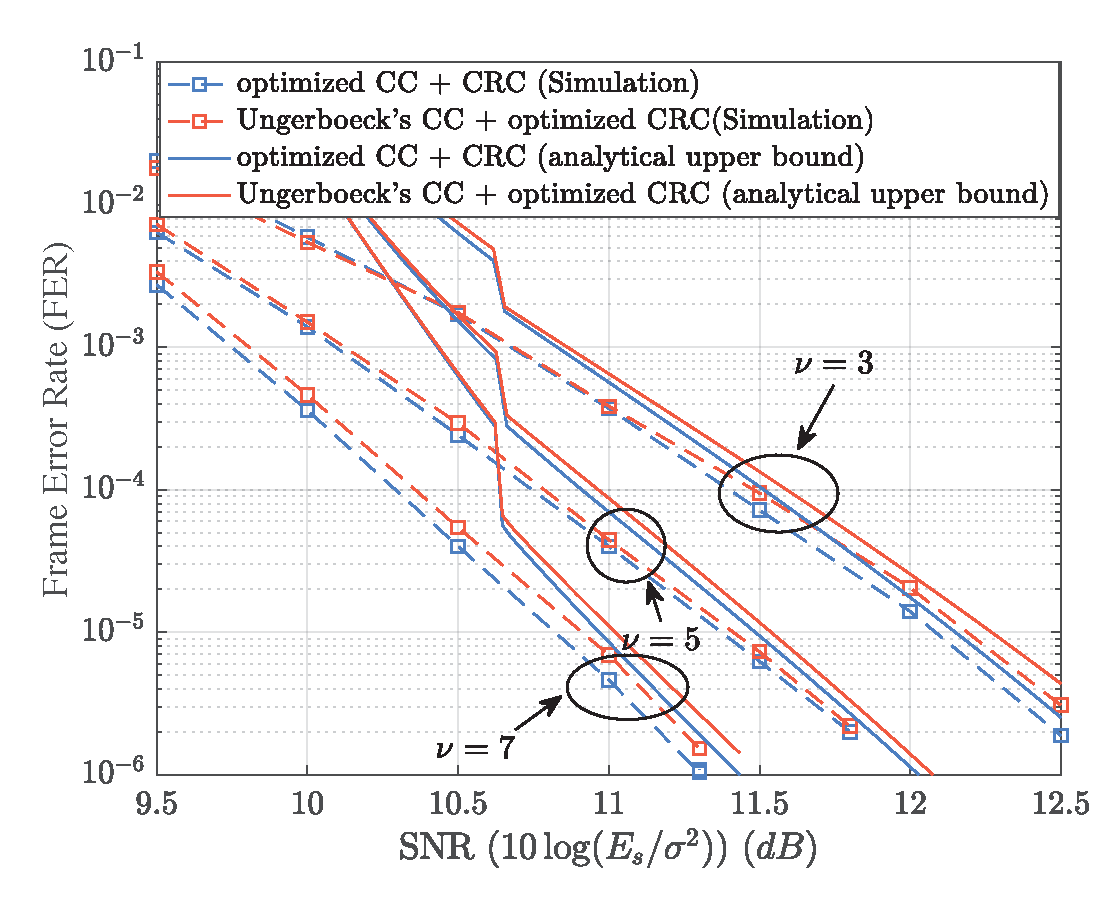
\includegraphics[width=0.6\linewidth]{figures/Figure_1_analytical.eps}
      \caption{The upper bounds and FER simulations of the simplified CRC-TCM-PAS system with a degree-2 CRC. The simplified system takes length-64 i.i.d. 4-ary amplitude symbol sequences and generates length-65 8-AM symbol sequences.  }
      \label{fig: unionbound}
\end{figure}

\begin{figure}[t] 
    \centering
      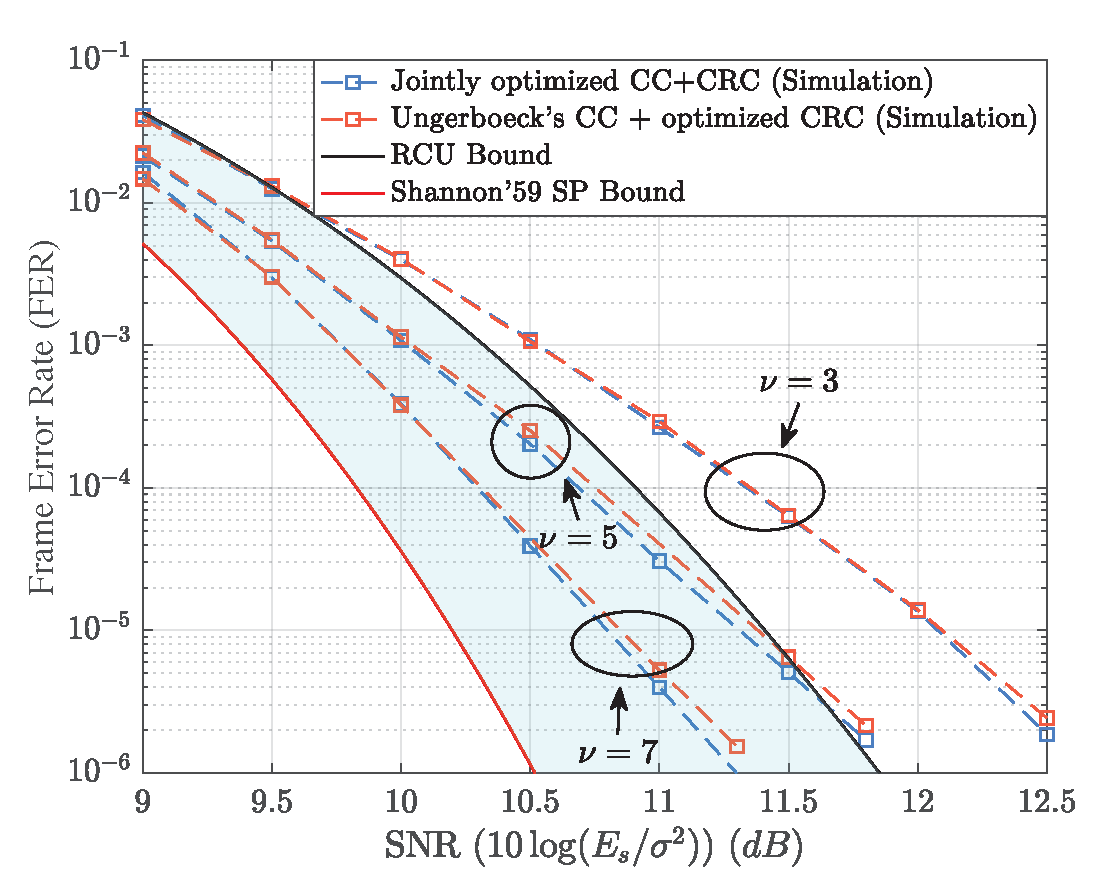
\includegraphics[width=0.6\linewidth]{figures/Figure_2_Simulation.eps}
      \caption{The FER curves of the practical  CRC-TCM-PAS transmission system that uses MCDM with $\mathcal{C}_{\mathrm{HP}}$. This system takes 87 input bits and generates 65 8-AM symbols. }
      \label{fig: fer_1}
\end{figure}

\begin{figure}[t] 
    \centering
      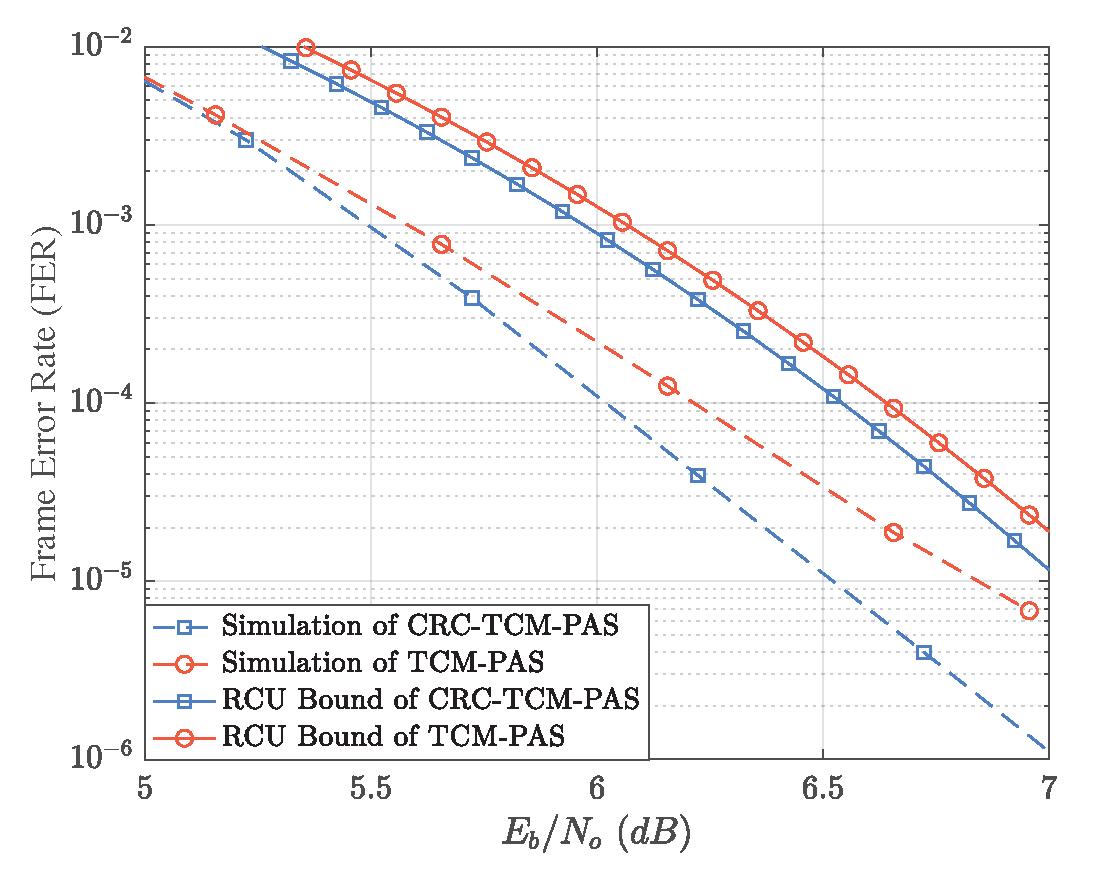
\includegraphics[width=0.6\linewidth]{figures/remove_CRC.eps}
      \caption{The FER curves and RCU bounds of the CRC-TCM-PAS system and TCM-PAS system. The gap between the two curves indicates the contribution of the 2-bit CRC. This system takes 87 input bits and generates 65 8-AM symbols. }
      \label{fig: remove_crc}
\end{figure}

Fig. \ref{fig: unionbound} presents analytical upper bounds and simuulation results that compare FERs for the optimized convolutional codes to  Ungerboeck's convolutional codes for a CRC-TCM-PAS system that assumes an ideal DM.  Hence, the system input "messages" are length-64 i.i.d. magnitude symbol sequences according to the PMF $P(\hat{A})$. The magnitude sequences are encoded and modulated by CRC-aided TCM to length-65 8-AM symbol sequences. Simulation results show that maximizing the FER upper bound finds slightly better convolutional codes  than those in Ungerboeck's paper.  Note that in both cases the FER upper bound was used to optimize the CRC polynomial.

The system uses TBCCs and CRCs from Table \ref{tab:OptimCodes}.
 The receiver uses an ML decoder. 
%Fig. \ref{fig: fer_1} uses the CC and CRC parameters optimized in Fig. \ref{fig: unionbound}.
Shannon's 1959 sphere packing (SP) bound \cite{shannon1959probability}  and Polyanskiy's random coding union (RCU) bound \cite{polyrcu} are also shown. Note that the last channel input of the CRC-TCM-PAS system is uniform \cite{wang2021achieving}. When calculating the RCU bound, we assume all channel inputs have the DM output distribution.  Fig. \ref{fig: fer_1} shows that, when a practical DM is considered,  the optimized convolutional codes deliver a slightly better performance than Ungerboeck's convolutional codes. When $\nu=7$, the FER performance  of  the CRC-TCM-PAS system with optimized CRC and TBCC is better than RCU bound by 0.55 dB at the FER of $10^{-6}$. Note that the FER curves from the simulation with the ideal DM in Fig. \ref{fig: unionbound} are similar to those with the real DM in Fig. \ref{fig: fer_1}.

Fig. \ref{fig: remove_crc} evaluates the contribution of the 2-bit CRC of the CRC-TCM-PAS system with $\nu=7$ TBCC in  Fig. \ref{fig: fer_1}. We refer to the system without CRC as the TCM-PAS system.
Hence, the TCM-PAS system takes 87 input bits and generates 64 8-AM symbols.
The FER curve and the RCU bound for the two systems are given in Fig. \ref{fig: remove_crc}.  It can be seen that the  CRC-TCM-PAS system outperforms the TCM-PAS system by about 0.3 dB at the FER of $10^{-5}$, which implies the importance of the 2-bit CRC.

\begin{figure}[htp] 
    \centering
  \subfloat[\label{fig: fer_sub_decoder}]{%
       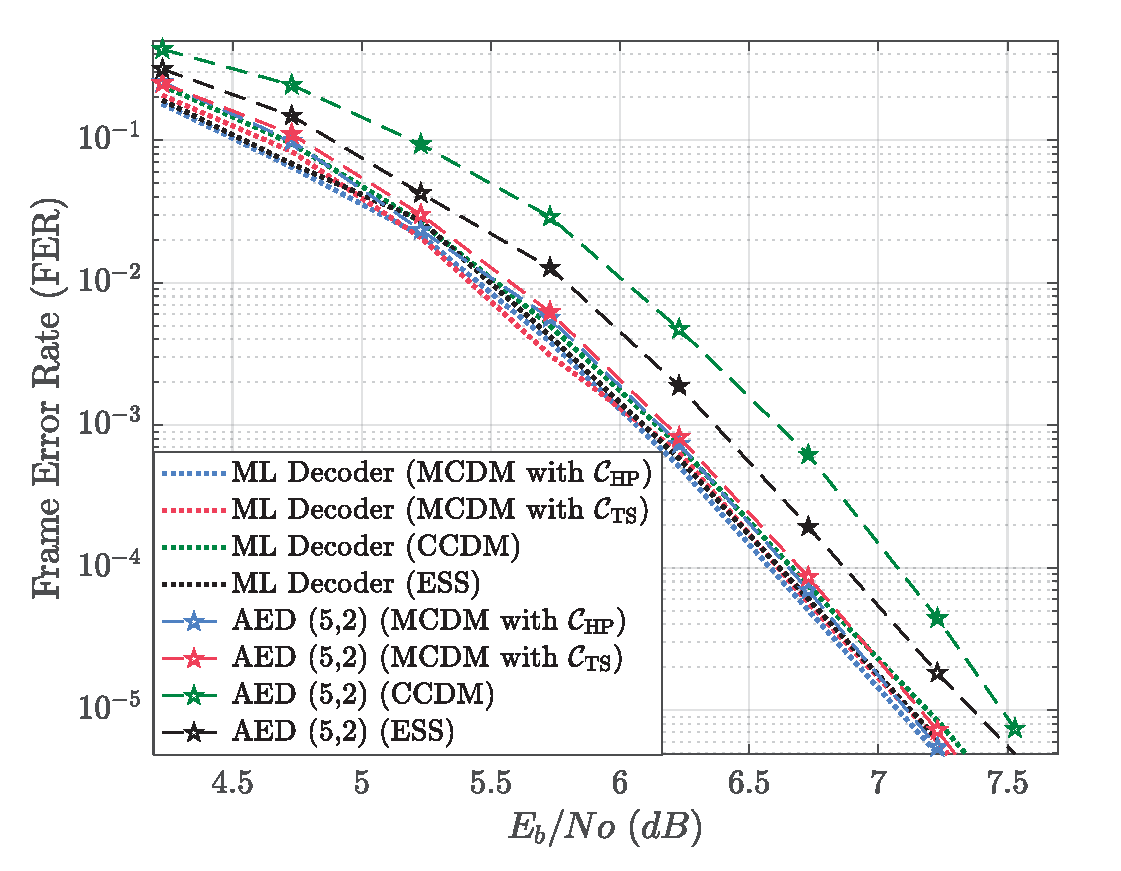
\includegraphics[width=0.5\linewidth]{figures/DM_FER.eps}}
   \\
  \subfloat[\label{fig: ls_sub_decoder}]{%
        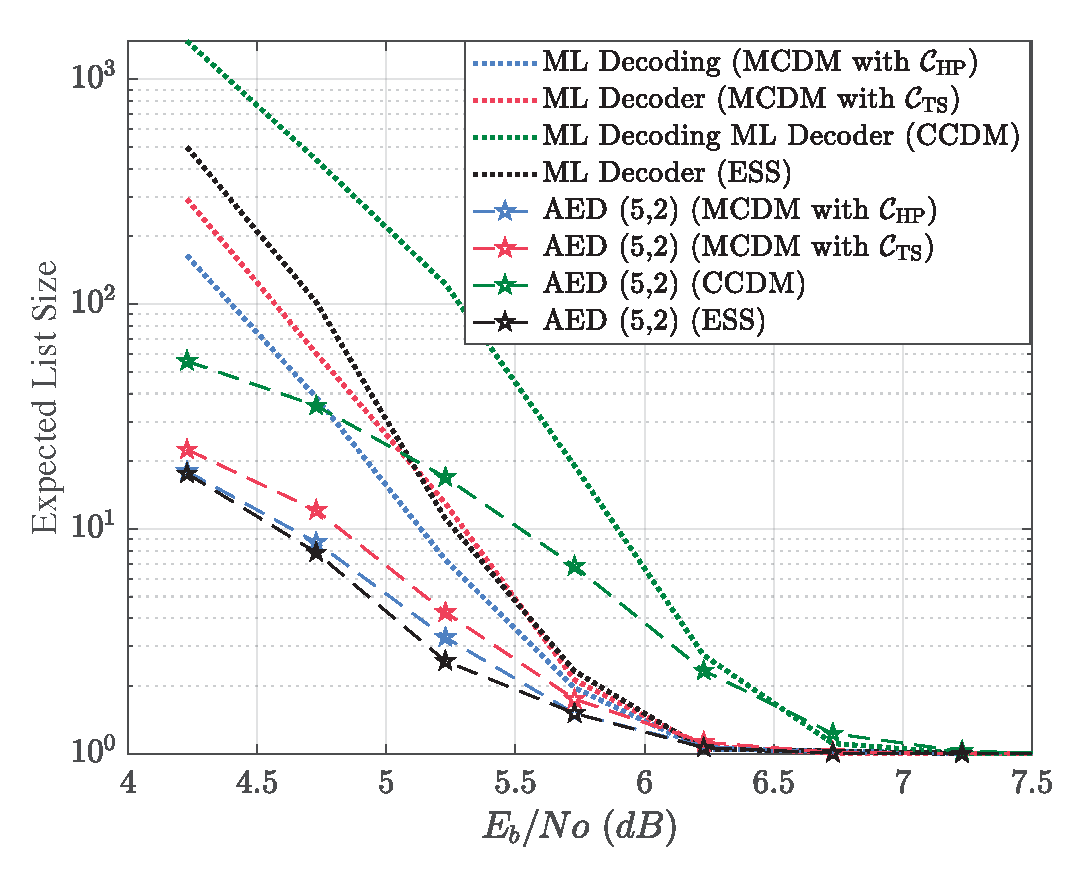
\includegraphics[width=0.5\linewidth]{figures/DM_listsize.eps}}
  \caption{ The performance of a CRC-TCM-PAS transmission system with various DMs and decoders. The system takes 96 input bits and generates 64 output symbols. Fig. (a) and (b) give the FER and expected list size, respectively.} \label{fig: sub}
\end{figure}


\begin{figure}[htp]
    \centering
    \subfloat[\label{fig: final_comp}]{%
        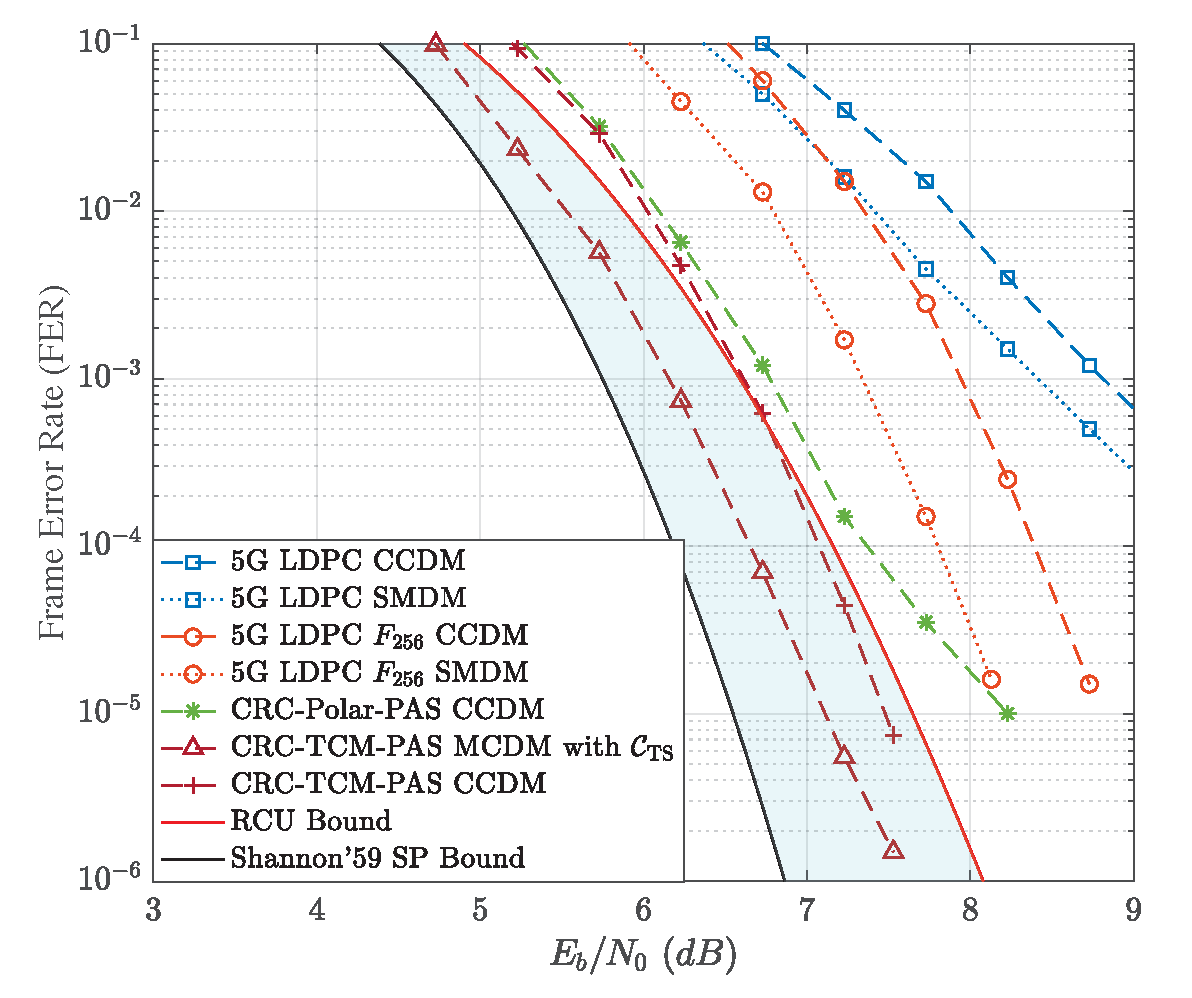
\includegraphics[width=0.5\linewidth]{figures/various_code_comparison.eps}}
    \\
    \subfloat[\label{fig: various_rate}]{%
        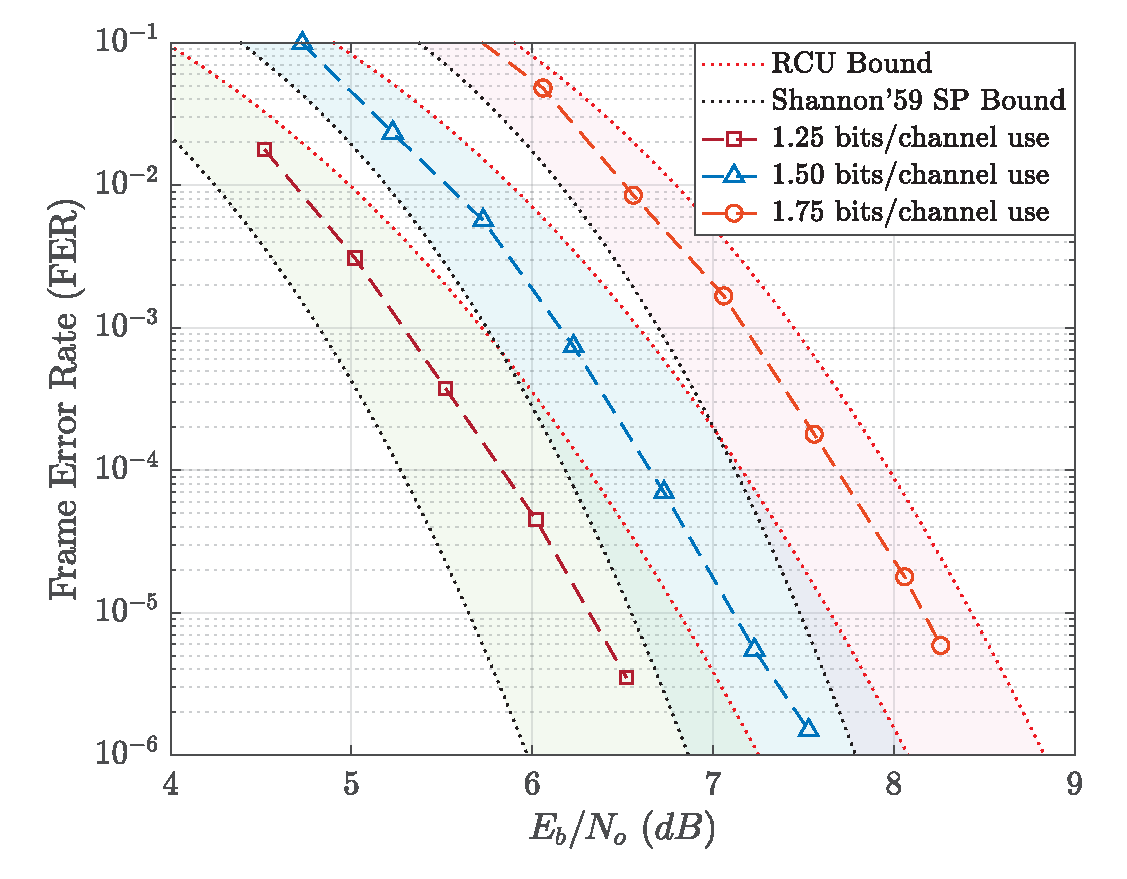
\includegraphics[width=0.5\linewidth]{figures/various_rates.eps}}
    \caption{(a): The FER curves of PAS systems with different FECs. All the PAS systems generate 64 8-AM symbols with a transmission rate of 1.5 bit/real channel use.  The CRC-TCM-PAS system utilizes CCDM and MCDM with $\mathcal{C}_{\mathrm{TS}}$ as the DM. The decoder of the CRC-TCM-PAS system is AED(5,2) with a maximum list size of 100. (b): The FER curves of CRC-TCM-PAS systems with various rates. The CRC-TCM-PAS systems generate 64 8-AM symbols, with  transmission rates of 1.25, 1.5, and 1.75 bit/real channel use, respectively.
    }
\end{figure}

Fig. \ref{fig: sub} investigates the CRC-TCM-PAS system that uses various DMs and two decoders, ML decoding and a sub-optimal but less complex AED(5,2) decoder. The system in Fig. \ref{fig: sub} has $k=96$ input bits and $n=64$ output symbols, and the transmission rate is $1.5$ bits/real channel use. The CRC-aided TCM uses the jointly optimized $\nu=7$, rate-$2/3$ TBCC, and the 2-bit CRC in Table \ref{tab:OptimCodes}. Fig. \ref{fig: fer_sub_decoder} and \ref{fig: ls_sub_decoder} give the FER performances and expected list sizes, respectively. 



We first investigate the performances of the CRC-TCM-PAS systems with various DMs and the ML decoder. The simulation results show that the four considered distribution matchers, i.e., ESS, CCDM, MCDM with $\mathcal{C}_{\text{HP}}$ and $\mathcal{C}_{\text{TS}}$  deliver similar FER performances under ML decoding. However, the CCDM requires more list size than the other three DMs. Fig. \ref{fig: sub} also presents the FER performance when the AED(5,2) is used. The maximum list size of all $2$-States decoders in AED(5,2) is 100. As shown in Fig. \ref{fig: sub}, when AED(5,2) is used as the decoder, the CRC-TCM-PAS system with CCDM delivers the worst FER and largest expected list size. On the other hand, the  CRC-TCM-PAS systems that use the MCDM with $\mathcal{C}_{\mathrm{HP}}$ and $\mathcal{C}_{\mathrm{TS}}$ deliver the near-optimal FER performance and outperform the system that uses ESS.

Fig. \ref{fig: final_comp} compares the decoding performance of CRC-TCM-PAS system with other PAS systems that use various FEC codes in \cite[Fig.14]{cocskun2019efficient}. All systems have 96 input bits, and the transmission rate is $1.5$ bits/real channel use. 
For the CRC-TCM-PAS, two distribution matchers are considered, i.e., MCDM with $\mathcal{C}_{\mathrm{TS}}$ and CCDM. The decoder uses AED(5,2) with a maximum list size of 100.
The details of  other PAS systems are described in   \cite{cocskun2019efficient}. The simulation results show that the CRC-TCM-PAS system with MCDM delivers the best performance and outperforms the CRC-Polar-PAS system by nearly 1dB.  Since the CRC-Polar-PAS system uses CCDM as the distribution matcher, the gain of CRC-TCM-PAS over CRC-Polar-PAS can come from two factors: the choice of DM or the coded modulation scheme. As shown in Fig. \ref{fig: final_comp}, with CCDM as the distribution matcher, the CRC-TCM-PAS system still outperforms the CRC-Polar-PAS system but does not perform as well as CRC-TCM-PAS with MCDM. Notably, the CRC-TCM-PAS system doesn't display the error floor of the CRC-Polar-PAS system, which shows an error floor at FER of $10^{-5}$. Hence, the gap between the FER curves of the CRC-TCM-PAS with CCDM and the CRC-Polar-PAS with CCDM can be treated as the gain of CRC-TCM code over CRC-Polar code, and the gap between the FER curves of the CRC-TCM-PAS with CCDM and the MCDM can be treated as the gain of MCDM over CCDM.

The error floor seen in the CRC-Polar-PAS with CCDM could be due to a variety of factors.  One factor is the sub-optimality in the decoder. Serial list Viterbi decoding of CRC-TBCC either chooses the ML codeword or reports an erasure with each growing list size.  In contrast,  successive cancellation list (SCL) decoding of CRC-polar codes sometimes selects non-ML codewords with a fixed list size of 32.
Thus, CRC-polar codes decoded using adaptive list sizes will display an error floor if the initial list size is small.
If the list size is fixed at a value such as 32, then performance will be limited by that small list size.
For polar codes, list sizes larger than 32 are typically not considered because of complexity limitations.
The error floor could also be due to a CRC that is too short, not optimized for high SNR, or otherwise sub-optimal.

Fig. \ref{fig: various_rate} evaluates the CRC-TCM-PAS system with various transmission rates. We design three CRC-TCM-PAS systems that take 80, 96, and 112 information bits, respectively, and generate 64 8-AM symbols. The resultant transmission rates are 1.25, 1.50, and 1.75 bits/real channel use, respectively. We design the MCDM with $\mathcal{C}_{\text{HP}}$ for all three transmission rates as distribution matcher. All three transmission rates employ the $\nu=7$ CC and the 2-bit CRC in Table \ref{tab:OptimCodes}. AED(5,2) with a maximum list size of 100 is used as the decoder.
%for all transmission rates. 
Fig. \ref{fig: various_rate} gives the FER curves, as well as the RCU bound and Shannon's 59 SP bound, of all three transmission rates. The simulation result shows that the FER curves for all three rates lie between the RCU and the SP bound, which indicates excellent decoding performance.

\section{Conclusion}\label{sec: conclusion_3}
Shannon's proof of the channel coding theorem \cite{shannon1948mathematical} generates a random codebook that has an optimal distribution and then performs an expurgation to improve the codebook.  The CRC-TCM-PAS system described in this paper follows that paradigm.  The DM plays the role of random codebook generation and the selection of that TCM and CRC polynomials expurgates that code to make it stronger. While there are many recent PAS systems, CRC-TCM-PAS allows the use of the tight FER upper bound derived in this paper for a precise expurgation of the codebook produced by the DM.  The TCM and CRC can be jointly selected to optimize FER performance.  This also paper proposes a new multi-composition DM (MCDM), which allows codewords with different compositions.  The new MCDM provides a significant benefit when decoding complexity is limited.
%The magnitude symbol sequences generated by the DM are then encoded and modulated by a CRC-aided TCM. 
%The TCM module includes a rate-$\frac{\ccinnum}{\ccinnum+1}$, systematic TBCC, and a channel-signal mapping function. This paper proves that, asymptotically, the distribution of the sign values produced by the TCM is equally likely. Hence, the channel inputs of the CRC-TCM-PAS system have a symmetric capacity-approaching distribution.
%Additionally, various decoders for the CRC-TCM-PAS system are studied in this paper.
Simulation results show that the optimized CRC-TCM-PAS system with MCDM exceeds the RCU bound for a variety of rates and outperforms the PAS systems with various FEC codes studied in \cite{cocskun2019efficient}.


\chapter{Rate-Matched Turbo Autoencoder: A Deep Learning Based Multi-Rate Channel Autoencoder} \label{cpt: cae}

\section{Introduction}
Channel codes  are important components of modern digital communication systems since they enhance transmission reliability. Capacity-approaching channel codes, such as low-density parity-check (LDPC) code\cite{gallager1962low}, polar code\cite{Arikan_polar}, and turbo code\cite{turbo}, have been used as standards for fourth-generation (4G) or fifth-generation (5G) wireless communication systems \cite{3gpp.36.212, 3gpp2017study}.

Recently, there has been a growing interest in designing channel codes using deep learning. For example, \cite{nachimain_ldpc_neural_decoder,wang_n2dnms,polar_neural_decoder} used deep neural networks to improve the error correction performances of the decoders for LDPC and polar codes.
The other research direction is designing the neural channel codes \cite{makkuva2021ko,chahine_tae_interleaver,clausius_strcutre_tae,jamali_productae,jiang_rnn_cae,saber_list_tae,jiang2019turbo,zhang2021design}. Neural channel codes apply the autoencoder framework \cite{vincent2008extracting} to the code design, i.e., the encoder and decoder are replaced with neural networks. The neural encoder and decoder can  thus be learned by optimizing the weights and biases of the neural networks. 
%Such channel codes are often referred as to channel autoencoders.

In \cite{jiang2019turbo}, Jiang \emph{et al.} proposed the turbo autoencoder (TAE). TAE mimics the structure of the traditional turbo code but replaces the convolutional code encoders and soft-input-soft-output decoders with neural networks. TAE delivers a comparable bit error rate (BER) to the state-of-art codes such as LDPC and Polar codes. 

Some techniques have been proposed to further improve the performance of TAE. Chahine \emph{et al.} in \cite{chahine_tae_interleaver} and Yildiz \emph{et al.} in \cite{TAE_interleaver} optimized the interleaver of the TAE. In \cite{saber_list_tae}, Saber \emph{et al.} proposed a list autoencoder that allows the decoder to generate multiple decoded message words, and choose the one that passes the cyclic redundancy check. 

In wireless communication systems, in order to adapt to the channel conditions, rate matching is widely used to match the number of transmitted code symbols to a desired rate. For the linear block codes, rate matching is realized by creating a new code with desired rate from a mother code using one or more bit-level operations such as extending, puncturing, and expurgating\cite{blahut2003algebraic}. It is crucial for the rate matched code to provide excellent error correction performances across different rates. In this work, we study the rate-matching problem of TAE and propose rate matching schemes to optimize the performance across multiple rates. In our proposed framework, the rate-matched TAE employs a ($3k,k$) TAE as the mother code, and adjusts the code rate by using a combination of freezing message bits, repeating code symbols, and puncturing code symbols. 

\section{Contribution}
The contributions of this paper are summarized as follows:

\begin{itemize}
    \item \textit{Rate-matched TAE.} The rate-matched TAE supports any message word length that is less than or equal to the message word length of the mother TAE and any arbitrary code length. We refer to the conventional TAE that is optimized for the message word length $k$ and code word length $3k$ as mismatched TAE. The rate-matched TAE shares the same encoder and decoder structure with mismatched TAE but is trained to jointly optimize the performance across all the rates of interest. The proposed rate matching operations in this paper can be generalized to any AE model. 
    \item \textit{Training signal-to-noise ratios (SNRs) optimization.} As reported in \cite{jiang2019turbo}, the variance of the noise added to the code words during the training process plays an important role for the code performance. With rate-matched TAE, different code rates require noise with different SNRs. To determine the training SNRs for each rate, a heuristic algorithm is proposed that uses test loss as a performance metric.
    \item \textit{Puncturing pattern investigation.} It is well-known that puncturing patterns affect the performance of the classical turbo codes. We propose and evaluate three puncturing patterns, namely, head, tail, and uniform puncturing, for the rate-matched TAE.
\end{itemize}


\subsection{Organization}
The remainder of this paper is organized as follows: Section \ref{sec: auto_enc} presents the encoder and decoder of TAE. Section \ref{sec: rate_matched_TAE} gives the framework of the rate-matched TAE; this section also presents the algorithm for determining the training SNRs for each considered code rate. Section \ref{sec: simulation} gives the simulation results of rate-matched TAE.  Section \ref{sec: conclusion_5} concludes the paper. 

\section{Turbo Autoencoder}\label{sec: auto_enc}
TAE is a deep-learning-based channel code with comparable error correction performance with state-of-art codes like LDPC and Polar codes for short to moderate block lengths, e.g., $K=100$ \cite{jiang2019turbo}. 
In this section, we present the encoder and decoder of TAE. 

\subsection{TAE Encoder}
Let $\mathbf{u}$ be a length-$k$ message word to be transmitted. A continuous rate-$\frac{1}{3}$ TAE encodes $\mathbf{u}$ as follows:
\begin{align*}
   \mathbf{x}_1&=h\left(f_{{\boldsymbol\theta}_1}(\mathbf{u})\right), \\
   \mathbf{x}_2&=h\left(f_{{\boldsymbol\theta}_2}(\mathbf{u})\right), \\
   \mathbf{x}_3&=h\left(f_{{\boldsymbol\theta}_3}(\mathbf{\pi(u)})\right),
\end{align*}
where $\pi(\cdot)$ is an interleaver. $f_{{\boldsymbol\theta}_i}(\cdot)\in\mathbb{R}^{k}$ is a the output of a neural network model with learnable parameters  ${\boldsymbol\theta}_i$, $i=1,2,3$. The model corresponding to each $f_{\boldsymbol\theta_i}(\cdot)$ is comprised of an  $l_{\text{enc}}$-layer convolutional neural network (CNN) with  $f_{\text{enc}}$  kernels of size $s_{\text{enc}}$ and a fully-connected neural network (FCNN) to match the output size. The code words of TAE are real-valued, so the TAE can be seen as a coded modulation scheme. Let $\mathbf{x}_i=[x_{i,1},x_{i,2},\allowbreak\ldots,x_{i,k}]$ for $i=1,2,3$. The function $h(\cdot)$ is the power normalization function \cite{jiang2019turbo} such that:
\begin{align}
    \frac{1}{k}\sum_{j=1}^{k}x_{i,j}&=0,&
    \frac{1}{k}\sum_{j=1}^{k}x^2_{i,j}&=1\label{equ: power_normalization},
\end{align} 
for $i=1,2,3$. 

We use $\mathbf{x}=f_{\pi,{\boldsymbol\theta}}(\mathbf{u})$ to denote the TAE encoder function, where $\mathbf{x}=[\mathbf{x}_1,\mathbf{x}_2,\mathbf{x}_3]\in\mathbb{R}^{n}$ is the length-$n$ code word, and $n=3k$. Denoting a code with message word length $k$ and code length $n$ as an $(n,k)$ code, the code rate is defined as $r=k/n$. The TAE is a rate $1/3$ code \cite{jiang2019turbo}.
\begin{figure*}[t] 
    \centering
      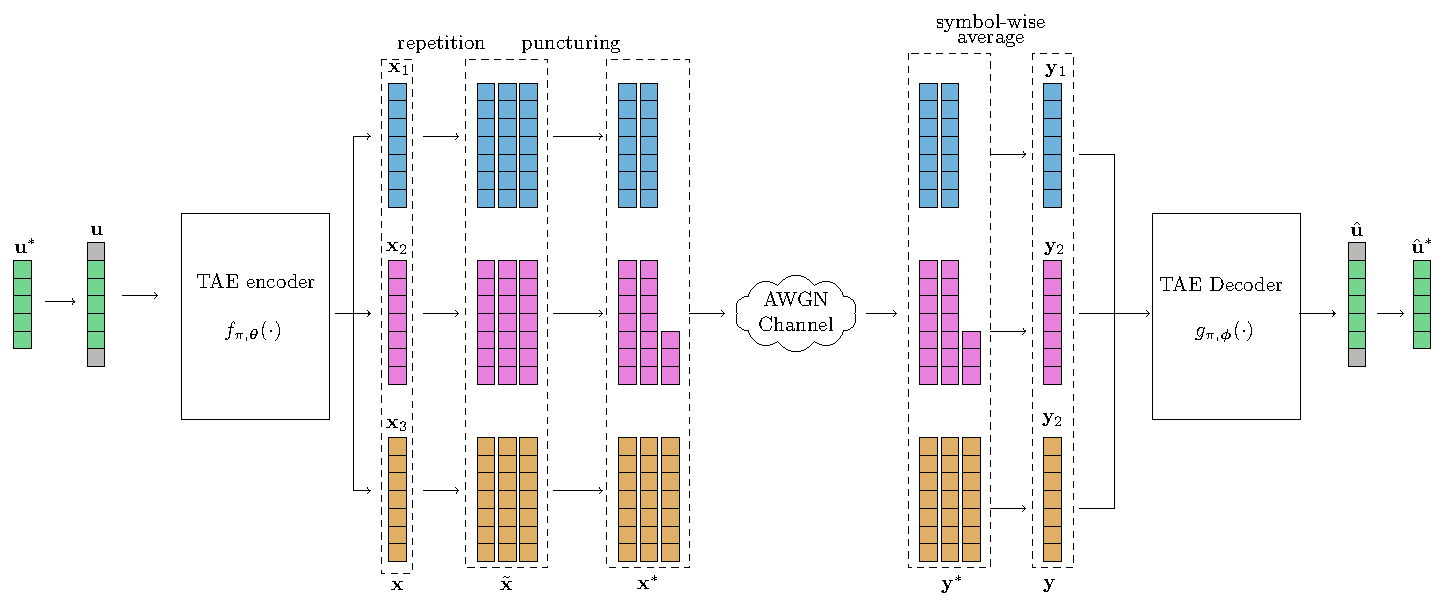
\includegraphics[width=1\linewidth]{figures/structure.pdf}
      \caption{The diagram of rate-matched TAE transmission system. The base code is a rate-$1/3$ TAE, and various rates are realized by freezing data symbols, repeating code symbols, or puncturing code symbols.}
      \label{fig: rate_match_framework}
\end{figure*}

\subsection{TAE Decoder}
Let $\mathbf{y}=[y_1,\ldots,y_n]$ be the channel observation at receiver when transmitting a code word $\mathbf{x}$. Considering an  additive white Gaussian noise (AWGN) channel,
\begin{align*}
    y_i=x_i+z_i,
\end{align*}
where $i=1,...,n$ and $z_i$ is a realization of Gaussian distribution $\mathcal{N}(0,\sigma^2)$. Since \eqref{equ: power_normalization} guarantees that the averaged symbol power of $\mathbf{x}$ equals to 1, the SNR in dB is conveniently defined as $10\mathrm{log}_{10} {1}/{\sigma^2}$.

For the rate-${1}/{3}$ TAE, $\mathbf{y}$ can be uniformly split into three sub-vectors, i.e., $\mathbf{y}=[\mathbf{y}_1,\mathbf{y}_2,\mathbf{y}_3]$, where $\mathbf{y}_i$ is the  channel observation corresponding to $\mathbf{x}_i$. The TAE decoder is an iterative decoder with $T$ iterations. In iteration $t$, the decoder accepts an information matrix $\mathbf{P}_{t-1}$, from the previous iteration, and combines it with the channel observations, and computes the information matrix $\mathbf{P}_{t}$ that is either used to feed the next iteration or estimate code words. $\mathbf{P}_{t}$ is calculated as follows: 
\begin{align}  \mathbf{Q}_{t,1}&=g_{{\boldsymbol\phi}_{t,1}}(\mathbf{y}_1,\mathbf{y}_2,\mathbf{P}_{t-1})-\mathbf{P}_{t-1},\\
    \mathbf{Q}_{t,2}&=\left\{\begin{matrix}
     g_{{\boldsymbol\phi}_{t,2}}(\pi(\mathbf{y}_1),\mathbf{y}_3,\pi(\mathbf{Q}_{t,1}))-\pi(\mathbf{Q}_{t,1})& t<T \\ 
     g_{{\boldsymbol\phi}_{t,2}}(\pi(\mathbf{y}_1),\mathbf{y}_3,\pi(\mathbf{Q}_{t,1})) &  t=T  \\
    \end{matrix}\quad,\right.\\ % \mathbf{Q}_{t,2}&=g_{{\boldsymbol\phi}_{t,2}}(\pi(\mathbf{y}_1),\mathbf{y}_3,\pi(\mathbf{Q}_{t,1})),\\
    \mathbf{P}_{t}&=\pi^{-1}(\mathbf{Q}_{t,2}),
    \end{align}
    where $\mathbf{Q}_{t,i}\in\mathbb{R}^{k\times f}$ for $t=1,...,T$, $i=1,2$, and $f$ is the information feature size for each code bit. $\mathbf{P}_t\in\mathbb{R}^{k\times f}$ for $t=0,\ldots T-1$, and $\mathbf{P}_T\in\mathbb{R}^{k}$. Also, $\pi^{-1}(\cdot)$ is the inverse interleaving operation. Each $g_{\boldsymbol{\phi}_{t,j}}(\cdot)$ consists of  an  $l_{\text{dec}}$-layer CNN with  $f_{\text{dec}}$  kernels of size $s_{\text{dec}}$ and an FCNN to match the output size.
    
    After $T$ iterations, the soft estimation for the  message word $\mathbf{u}$ is calculated using element-wise sigmoid operation;
    \begin{align}
        \hat{\mathbf{u}}=\text{sigmoid}\left(\mathbf{P}_T\right).
    \end{align}
    We use $\hat{\mathbf{u}}=g_{\pi,{\boldsymbol\phi}}(\mathbf{y})$ to denote the TAE decoder function.

    \section{Rate-Matched TAE}\label{sec: rate_matched_TAE}


    \subsection{Motivation}
    In practical applications such as 4G and 5G communication, it is desired to accommodate multiple code rates and lengths to adapt to channel varying conditions or the available transmission resources. One straightforward way to accommodate different rates is to design and employ multiple encoder and decoder pairs, one for each rate. However, this comes at the price of excessive hardware complexity and must be avoided. An alternative solution is to have a single encoder and decoder pair, and perform rate matching to match the code rate and length to the desired ones. Typically, an $(n,k)$ mother code with rate $r=k/n$ is designed, and a $(n^*,k^*)$ code with rate $r^*=k^*/n^*$ is constructed via rate matching of the mother code.
   
   
   To obtain a new linear block code with the desired code rate $r^*$, there are several rate matching operations that can be performed on the generator matrix $\mathbf{G}$ of a mother code. Some of these operations are listed in the following table. We refer readers to \cite[Chapter 3.6]{blahut2003algebraic} for more details.

   \begin{table}[h]
\centering
\begin{tabular}{|c|c|c|}
\hline
            & Operations to $\mathbf{G}$         & resultant code rate \\ \hline
Puncturing  & Eliminate columns in $\mathbf{G}$ & increased           \\ \hline
Extending   & Add columns in $\mathbf{G}$       & decreased           \\ \hline
Expurgating & Eliminate rows in $\mathbf{G}$    & decreased           \\ \hline
\end{tabular}
\end{table}
  
Although TAE is a non-linear code, and cannot be described by a generator matrix, similar operations can be used to obtain new codes from the TAE. We present a framework for a mother $(3k,k)$ TAE to match the desired code rate $r^*={k^*}/{n^*}$ for $k^*<k$. The TAE that is designed to support multiple rates is referred to as rate-matched TAE. 

\subsection{Rate-matched TAE Structure}\label{sec: rm_tae_structure}
Fig. \ref{fig: rate_match_framework} depicts the rate matching operation for the $(3k,k)$ TAE to an $(n^*,k^*)$ code with desired code rate $r^*={k^*}/{n^*}$. The rate-matching process can be summarized as follows:

\subsubsection{Zero Padding and Encoding} Let $\mathbf{u}^*\in\mathbb{F}_2^{k^*}$ ($k^*\leq k$) be the transmitted message word. Since the message word length of the mother TAE is $k$, $0$'s are padded to both sides of $\mathbf{u^*}$ to satisfy the input length requirement, i.e.,
\begin{align}\label{equ: padding}
    \mathbf{u}=[\underbrace{0~0\ldots 0}_{\left\lfloor\frac{\delta}{2}\right\rfloor }~\mathbf{u^*}~ \underbrace{0~0\ldots 0}_{\left\lceil\frac{\delta}{2}\right\rceil } ],
\end{align}
where $\delta=k-k^*$. In \eqref{equ: padding}, $\delta$ positions of $\mathbf{u}$ are frozen, and the remaining $k^*$ positions are filled with message bits. After zero padding, the TAE encoder encodes $\mathbf{u}$ to the code word $\mathbf{x}$ by $\mathbf{x}=f_{\pi,{\boldsymbol\theta}}(\mathbf{u})$.

\subsubsection{Repeating and Puncturing} The length of the mother TAE code word,   $\mathbf{x}=[\mathbf{x}_1,\mathbf{x}_2,\mathbf{x}_3]$, is $n$. To obtain a length-$n^*$ code word, we first extend the code word to length $pn$ using $p$ repetitions of $\mathbf{x}$, i.e.,
$$
    \tilde{\mathbf{x}}
    =[\mathbf{x}^{(1)},...,\mathbf{x}^{(p)}]\label{equ: rep}
    =[\mathbf{x}_1^{(1)},\mathbf{x}_2^{(1)},\mathbf{x}_3^{(1)},\ldots, \mathbf{x}_1^{(p)},\mathbf{x}_2^{(p)},\mathbf{x}_3^{(p)}],
$$
where $\mathbf{x}^{(i)}=\mathbf{x}$ and $\mathbf{x}_{j}^{(i)}=\mathbf{x}_j$ for $i=1,\ldots,p$ and $j=1,2,3$.
The number of repetition times, $p$, is calculated as
\begin{align}\label{equ: repe_time}
    p=\left\lceil{n^*}/{n}\right\rceil.  
\end{align}
In order to obtain the length-$n^*$ code word $\mathbf{x}^*$, $\beta=pn-n^*$ code symbols in $\tilde{\mathbf{x}}$ are punctured. \eqref{equ: repe_time} guarantees that $\beta<n$. Without loss of generality, we consider puncturing symbols in $\mathbf{x}^{(p)}$. 
In this paper, we consider the following three heuristic puncturing patterns. 

\begin{itemize}
    \item \textit{Head Puncturing.} The first $\beta$ symbols of $\mathbf{x}^{(p)}$, $x^{(p)}_{1},\ldots,\allowbreak x^{(p)}_{\beta}$, are punctured, where $x_i^{(p)}$ denotes the $i^{\text{th}}$ symbol in the vector $\mathbf{x}^{(p)}$.
    \item \textit{Tail Puncturing.} The last $\beta$ symbols of $\mathbf{x}^{(p)}$,  $x^{(p)}_{n-\beta+1},\ldots,\allowbreak x^{(p)}_{n}$, are punctured.
    \item \textit{Uniform Puncturing.} The first $\left\lfloor {\beta}/{3} \right\rfloor$ symbols of $\mathbf{x}_{1}^{(p)}$ and $\mathbf{x}_{2}^{(p)}$, and the first $\beta-2\left\lfloor {\beta}/{3} \right\rfloor$ symbols of $\mathbf{x}_{3}^{(p)}$ are punctured.
\end{itemize}

\subsubsection{Symbol-Wise Averaging and Decoding} Let $\mathbf{y}^*$ be the channel observation after transmission of $\mathbf{x}^*$ over AWGN channel. We perform symbol-wise averaging to obtain the input to the decoder, $\mathbf{y}$, i.e.,
\begin{align}
    y_i=\left\{\begin{matrix}
      \frac{1}{p_i}\sum_{j=1}^{p_i}y^{(j)}_i,&  p_i>0\\ 
      0, &  p_i=0 \\
     \end{matrix}\quad, i=1,\ldots,n. \right.\label{equ: quantization_mag}
\end{align}
$y_i^{(j)}$ is the receiver observation associated with $x^{(j)}_i$, and $p_i$ is the repetition number of code symbol $x_i$. Due to puncturing, we have $p_i\leq p$ for $i=1,\ldots, n$. 0's are filled to those positions with no transmitted symbols.

The decoder takes $\mathbf{y}$ as input, and calculates $\hat{\mathbf{u}}=g_{\pi,{\boldsymbol\phi}}(\mathbf{y})$. Finally, the soft estimation of $\mathbf{u}^*$, denoted by $\hat{\mathbf{u}}^*$, is given by
\begin{align}
    \hat{\mathbf{u}}^*= \left[\hat{u}_{\left\lfloor{\delta}/{2}\right\rfloor+1}\ldots \hat{u}_{\left\lfloor{\delta}/{2}\right\rfloor+k^*}\right].
\end{align} 

\subsection{Training Methodology}
Consider a rate-matched TAE that supports $q$ different rates, $r_1,\ldots, r_q$, where $r_i$ is specified by $k_i$ and $n_i$. As will be illustrated in Sec. \ref{sec: simulation}, the TAE that is designed  for message word length $k$ and $r=1/3$ may not work well for all $q$ rates. To optimize the performance across all rates, we train the rate-matched TAE with the batches that contain all $q$ rates.
\begin{figure*}[t] 
    \centering
      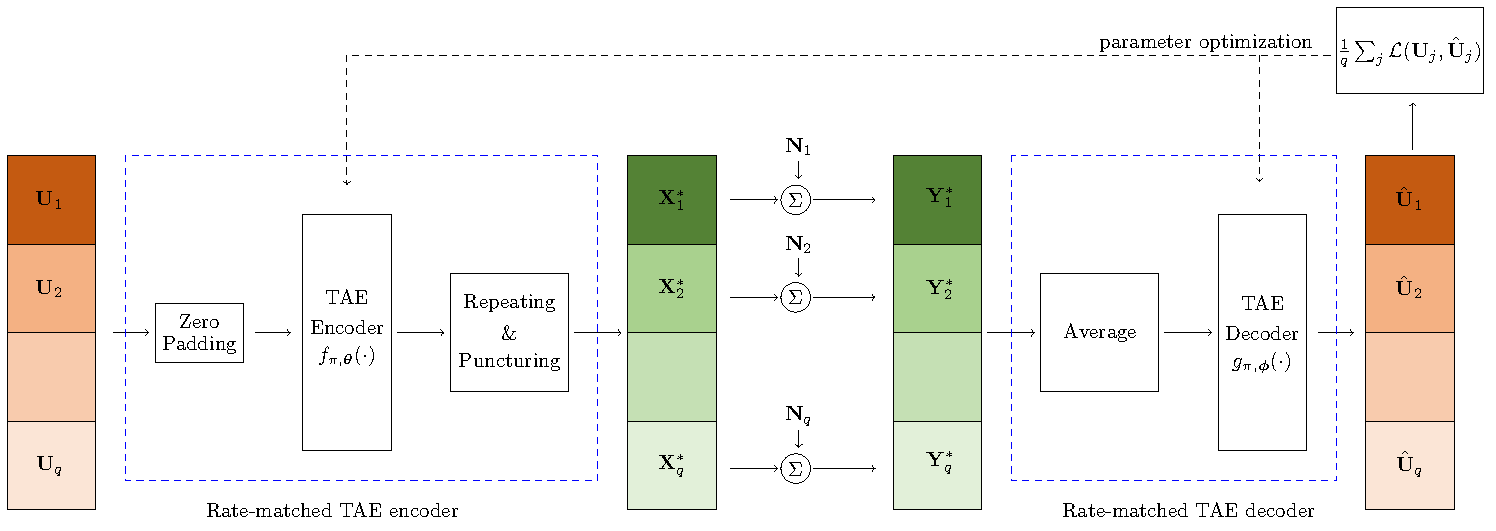
\includegraphics[width=1\linewidth]{figures/training_process.pdf}
      \caption{Training schedule for the rate-matched TAE.}
      \label{fig: training_process}
\end{figure*}
Fig. \ref{fig: training_process} visualizes the training process of rate-matched TAE. As shown in Fig. \ref{fig: training_process}, each batch contains $q$ sub-batches, $\mathbf{U}_1,\ldots, \mathbf{U}_q$, where $\mathbf{U}_j\in\mathbb{F}_2^{b\times k_j}$ contains $b$ randomly generated length-$k_j$ message words. We denote the batch size by $B=qb$. With the rate-matched TAE encoder, $\mathbf{U}_j$ is mapped to $\mathbf{X}^*_j\in\mathbb{R}^{b\times n_j}$ that contains $b$ code words of length $n_j$.

At the receiver end, the channel observation $\mathbf{Y}^*_{j}$ is generated by adding the randomly sampled noise $\mathbf{N}_j$ to $\mathbf{X}^*_j$, i.e.,
\begin{align}
    \mathbf{Y}^{*}_j=\mathbf{X}^{*}_j+\mathbf{N}_j.
\end{align}
The corresponding element to the $c^{\text{th}}$ column and $i^{\text{th}}$ row  in $\mathbf{N}_j$ is drawn from $\mathcal{N}(0,\tilde{\sigma}_{c,i}^2)$, where $\tilde{\sigma}_{c,i}^2$ is drawn from the uniform distribution between $10^{-0.1\alpha^{(j)}_{h}}$ and $10^{-0.1\alpha^{(j)}_{l}}$. Hence, $\mathbf{N}_j$ can be described by the \textit{training SNR} range $[\alpha_{l}^{(j)},\alpha_{h}^{(j)}]$. $\mathbf{Y}_j$ is then fed into the rate-matched TAE decoder to calculate the soft estimation of $\mathbf{U}_j$, i.e., $\hat{\mathbf{U}}_j\in\mathbb{R}^{b\times k_j}$. Finally, the total loss $J$ is calculated by $J=\frac{1}{q}\sum_{j=1}^{q}\mathcal{L}(\mathbf{U}_j,\hat{\mathbf{U}}_j)$, where $\mathcal{L}(\cdot,\cdot)$ denotes binary cross entropy (BCE) loss function.

We follow the same training schedule as \cite{jiang2019turbo}, which iteratively trains encoder and decoder. This helps avoid getting stuck in the local minima, and performs better than joint training. During each training epoch, the iterative training first optimizes the encoder $T_{\text{enc}}$ times by fixing the decoder parameters, and then optimizes the decoder $T_{\text{dec}}$ times by fixing the encoder parameters.

The training process for rate-matched TAE has two phases. First, coarse training is performed in which the model is trained from scratch for $E_{\text{cor}}$ epochs with a batch size of $B_{\text{cor}}$ and a learning rate $\ell_{\text{cor}}$. Second, we perform fine tuning in which the trained model from coarse training is used as initialization, and the model is trained for $E_{\text{fine}}$ epochs with a larger batch size $B_{\text{fine}}$ and a smaller learning rate $\ell_{\text{fine}}$.


\subsection{Training SNRs}
Similarly to train TAE in \cite{jiang2019turbo}, the encoder and decoder of rate-matched TAE are trained with different training SNRs. 
For a $q$-rate rate-matched TAE, the training SNR hyper-parameters are specified by $(\alpha^{(j)}_{\text{enc},l},\alpha^{(j)}_{\text{enc},h},\alpha^{(j)}_{\text{dec},l},\alpha^{(j)}_{\text{dec},h})$, for $j=1,...,q$. 
As can be seen, the hyper-parameter tuning becomes too complicated for large values of $q$. 
Therefore, we choose to reduce the number of hyper-parameters related to training SNRs by using the simplification in \cite{jamali_productae}: 
$\alpha^{(j)}_{\text{enc},l}=\alpha^{(j)}_{\text{enc},h}=\gamma^{(j)}$, $\alpha^{(j)}_{\text{dec},l}=\gamma^{(j)}-2.5$, and $\alpha^{(j)}_{\text{dec},h}=\gamma^{(j)}+1$.
% \begin{align*}    \alpha^{(j)}_{\text{enc},l}&=\alpha^{(j)}_{\text{enc},l}=\gamma^{(j)},
% \end{align*}
% \begin{align*}
%     \alpha^{(j)}_{\text{dec},l}&=\gamma^{(j)}-2.5,
% \end{align*}
% \begin{align*}
%     \alpha^{(j)}_{\text{dec},h}&=\gamma^{(j)}+1.
% \end{align*}
With this setting, the encoder training SNR for rate $j$ becomes a point at $\gamma^{(j)}$ dB, while the decoder training SNR for rate $j$ is an interval with length 3.5 dB whose boundaries are calculated based on $\gamma^{(j)}$. This setting is based on an observation of the optimized training SNR for a well-trained TAE in \cite{jiang2019turbo}. The above setting reduces the training SNR optimization to a $q$-dimensional searching space $\left(\gamma^{(1)},\ldots, \gamma^{(q)}\right)$.

As reported in~\cite{jamali_productae} and~\cite{jiang2019turbo}, the training SNRs are vital for a well-performed AE. %Based on the observation of training $r=k/3k$ TAE in \cite{jiang2019turbo}, 
To determine $(\gamma^{(1)},\ldots \gamma^{(q)})$, we propose a heuristic algorithm that uses the test loss after coarse training as a metric.
%that delivers a well-performed rate-matched TAE. 
We denote the test loss of rate $j$ after coarse training by $L^{(j)}_{\text{cor}}$, which is the BCE between an input batch $\mathbf{U}_j$ and corresponding $\hat{\mathbf{U}}_j$ after coarse training of rate-matched TAE with channel SNR $\gamma^{(j)}$ dB. The proposed algorithm finds $\left(\gamma^{(1)},\ldots \gamma^{(q)}\right)$ such that after coarse training, the test loss of all rates are in the designated range $[\epsilon_\text{l}, \epsilon_\text{r}]$. 

The algorithm starts with a randomly selected $(\gamma^{(1)},\ldots, \gamma^{(q)})$. At each iteration, coarse training is performed, and test loss are calculated. For all the rates $j$, $j=1,\ldots,q$, if the test loss $L^{(j)}_{\text{cor}}$ is in the desired range, $\gamma^{(j)}$ keeps unchanged. Otherwise, $\gamma^{(j)}$ is updated, i.e., if $L^{(j)}_{\text{cor}}<\epsilon_{\text{l}}$, $\gamma^{(j)}$ is decreased ; if  $L^{(j)}_{\text{cor}}>\epsilon_{\text{r}}$ , $\gamma^{(j)}$ is increased. This process is repeated until all $L_{\text{cor}}^{(1)},L_{\text{cor}}^{(2)},\ldots,L_{\text{cor}}^{(q)}$ fall into the designated range.
%The details of the algorithm are presented in Algorithm \ref{alg: snr_search}. 
Note that the proposed algorithm  doesn't guarantee the optimal $(\gamma^{(1)},\ldots \gamma^{(q)})$. However, it gives a rate-matched TAE with a satisfying performance. 

The intuition behind using the test loss function as a searching metric is that test loss reflects the noise level for encoder and decoder training SNRs. 
Both very large and very small noise variances in the training process will   fail to train a model with excellent error correction performance.  
% The loss that is too small and too large is not desired, as they indicate inappropriate noise levels.
We found that, for the TAE with $k=100$ and $n=300$, a well-performed model can be trained when the test loss is around $9*10^{-4}$ after coarse training. Hence, we relax the observed test loss to the range $[0.7,1.1]*10^{-3}$. It is noteworthy that tuning one $\gamma^{(j)}$ by fixing all other values could affect the performance of all rates since it changes the gradient calculation of the whole rate-matched TAE model. However, there is no deterministic relationship on how tuning one $\gamma^{(j)}$ impacts all other rates. 


\begin{figure}[t] 
    \centering
      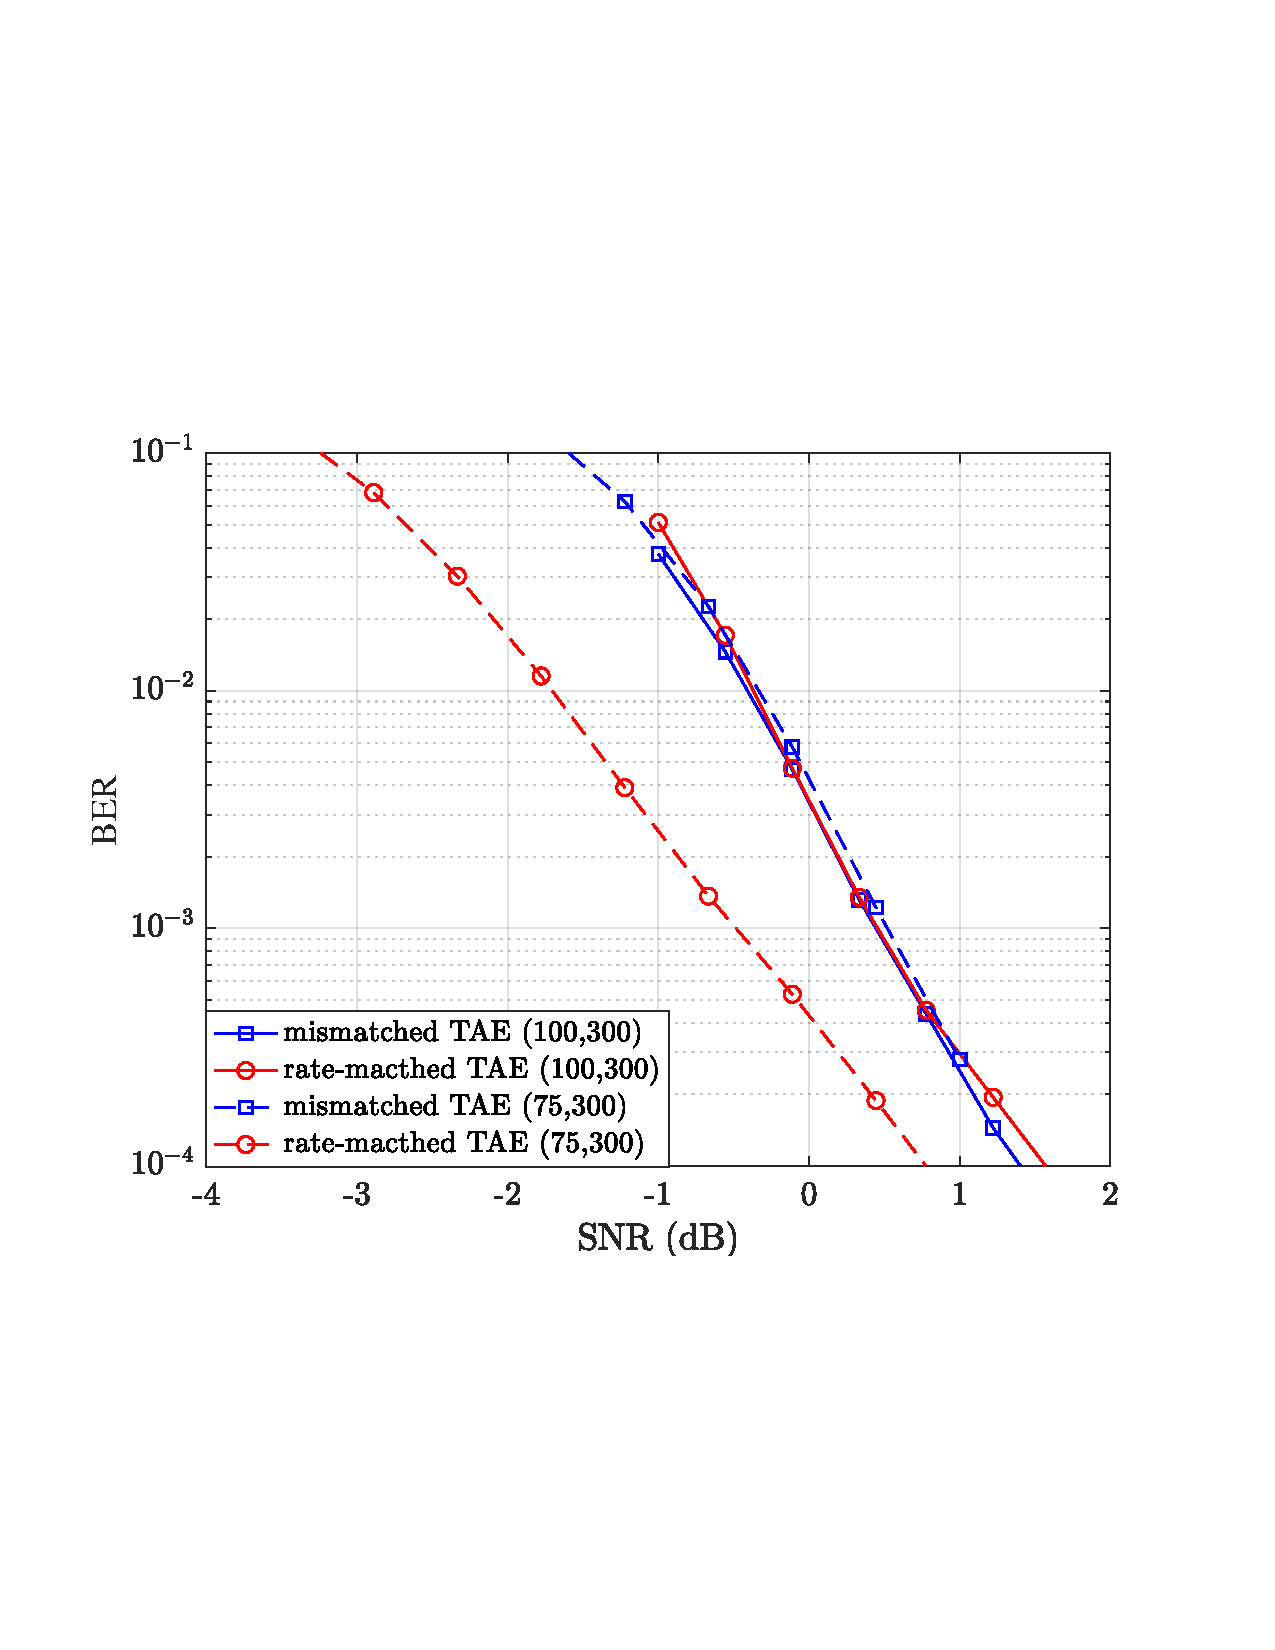
\includegraphics[width=0.5\linewidth]{figures/BER_75_300.pdf}
      \caption{The BER performance of rate-matched TAE that supports $k\in\{75, 100\}$ and $n=300$. The BER performance of mismatched TAE is also given for comparison.}
      \label{fig: FER_75_300}
\end{figure}
\begin{figure}[t] 
    \centering
      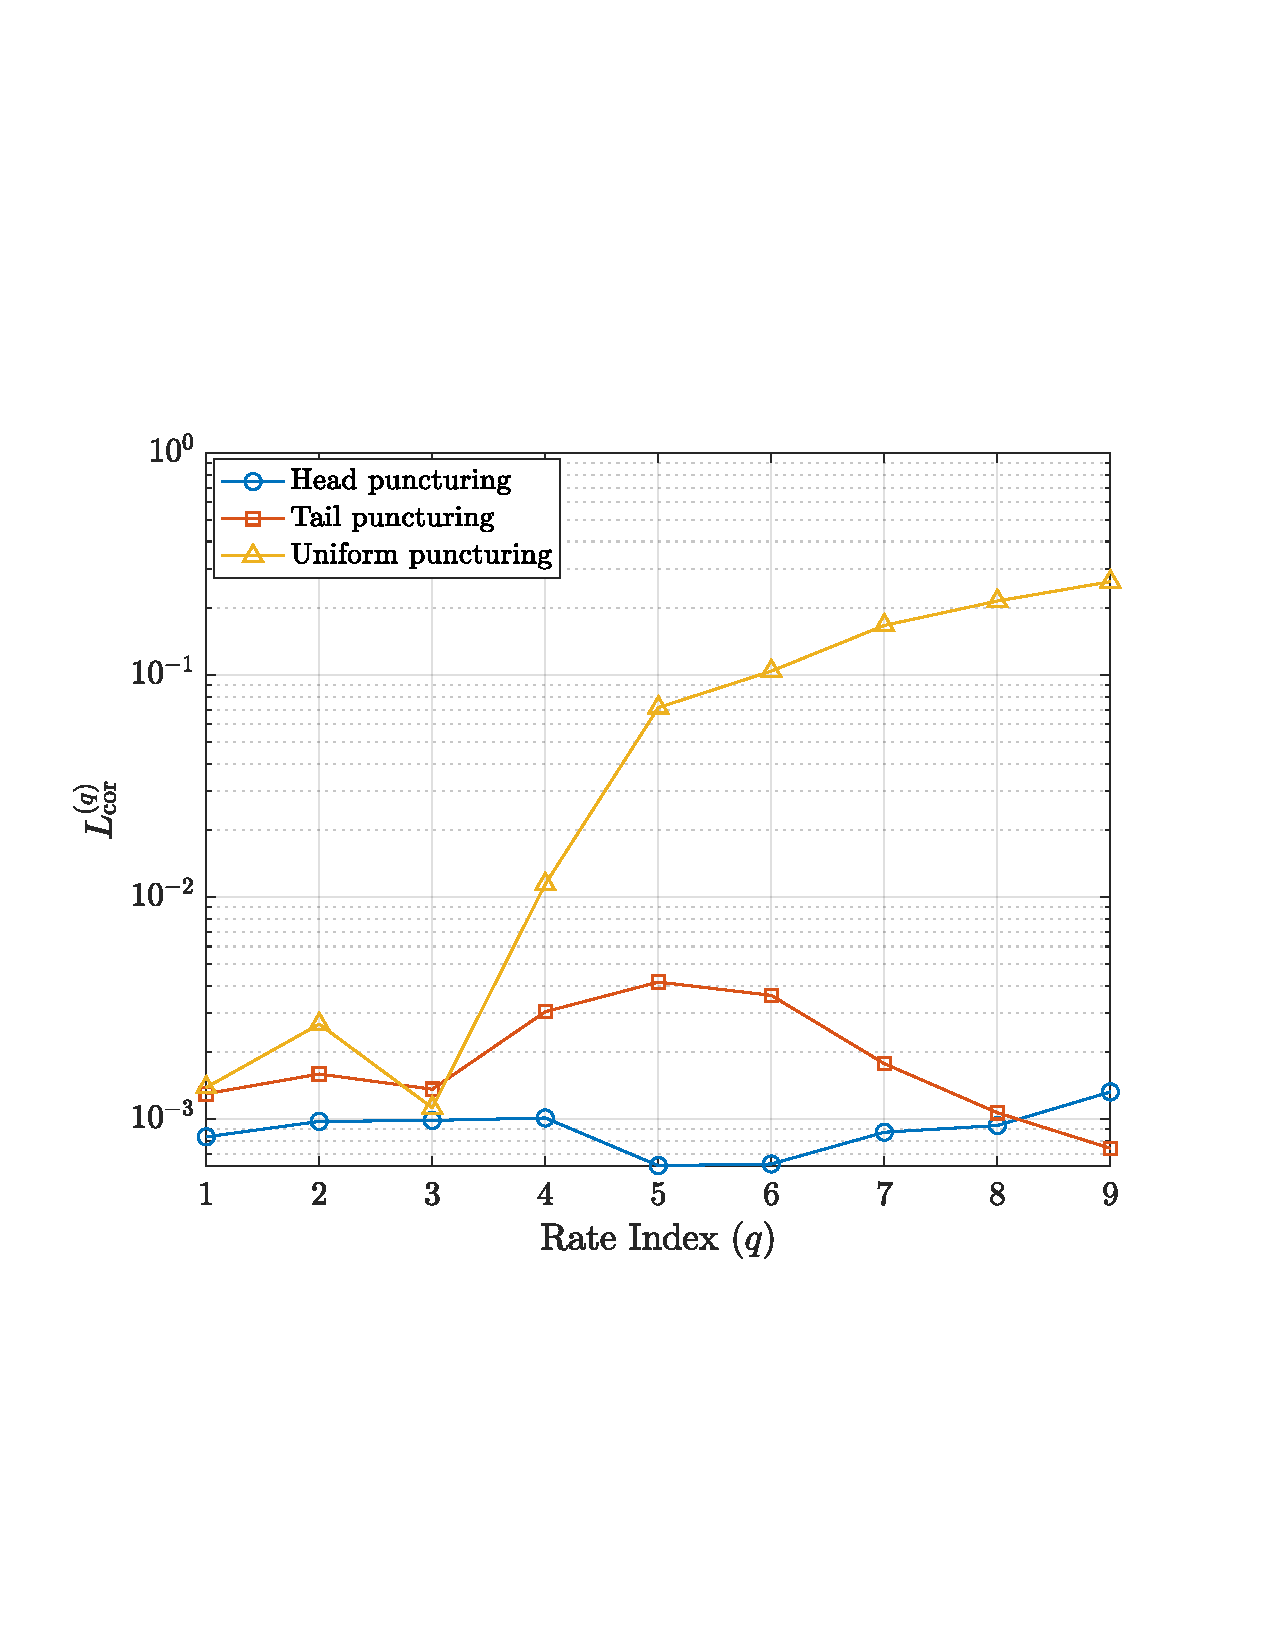
\includegraphics[width=0.5\linewidth]{figures/puncturing_invest.pdf}
      \caption{Test loss of rate-matched TAE with head, tail, and uniform puncturing after coarse training. The simulation results show that head puncturing delivers the best performance.}
      \label{fig: Validation_Loss}
\end{figure}
\begin{figure}[t] 
    \centering
      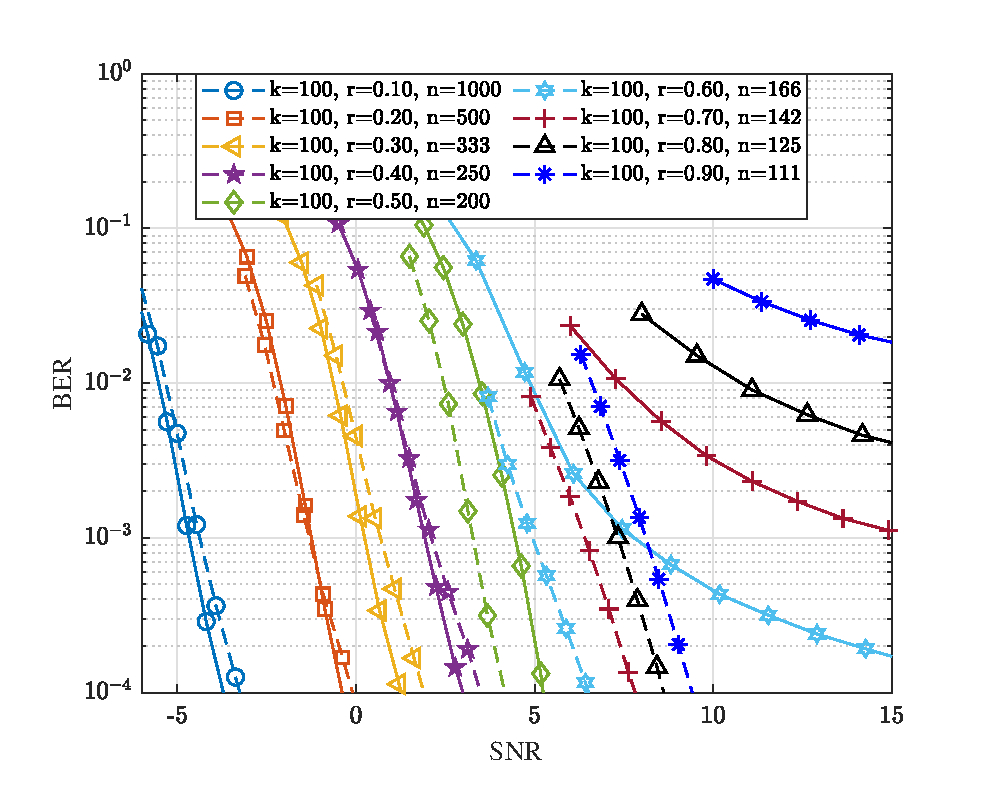
\includegraphics[width=0.5\linewidth]{figures/BER_size_1.eps}
      \caption{BER performance of the rate-matched TAE (dashed curves) and mismatched TAE (solid curves)  at all 9 code rates. The simulation results show that rate-matched TAE performs better at high rates.}
     \label{fig: BER_size_1}
\end{figure}

\section{Simulation Results}\label{sec: simulation}
%
In this section, we evaluate the performance of the rate-matched TAE. The mother code dimensions are $k=100$ and $n=300$. We train the rate-matched TAEs that support various rates, and compare them with the mismatched TAE that is specifically trained for $k=100$ and $n=300$. To ensure fair comparison, the rate-matched TAE and mismatched TAE have the same model size with $l_{\text{enc}}=2$, $\l_{dec}=5$, 
$s_{\text{enc}}=s_{\text{dec}}=5$, $f_{\text{enc}}=f_{\text{dec}}=100$, and $f=5$. The training hyper-parameters are listed below.
\begin{table}[h]
    \centering
    %\caption{\label{tab: training_schedule} Training Schedule for Rate-Matched and Mismatched TAE}
    \begin{tabular}{ll||ll}
    \hline
    Parameter                   & Value     & Parameter                    & Value     \\ \hline
    $B_{\text{cor}}$            & $540$     & $B_{\text{fine}}$             & $27000$   \\
    $E_{\text{cor}}$            & $1000$    & $E_{\text{fine}}$             & $300$     \\
    $\ell_{\text{cor}}$         & $10^{-4}$ & $\ell_{\text{fine}}$          & $10^{-5}$ \\
    $T_{\text{enc},\text{cor}}$ & $100$     & $T_{\text{enc},\text{fine}}$ & $2$       \\
    $T_{\text{dec},\text{cor}}$ & $500$     & $T_{\text{dec},\text{fine}}$ & $10$      \\ \hline
    \end{tabular}
\end{table}

We first consider a rate-matched TAE with $q=2$ rates, for $k\in\{75,100\}$ and $n=300$. The BER result in  Fig. \ref{fig: FER_75_300} shows that the rate-matched TAE outperforms the mismatched TAE for $k=75$, while having similar performance to the rate-matched TAE for $k=100$. 

We investigate the effect of different puncturing patterns for rate-matched TAE. The three puncturing patterns presented in Section \ref{sec: rm_tae_structure}, head puncturing, tail puncturing, and uniform puncturing, are considered in the rate-matched TAE training. All three puncturing patterns use the training SNRs in the above table.
We evaluate the rate-matched TAE with different puncturing patterns using the test loss of all 9 rates under the training SNRs $(\gamma^{(1)},\ldots,\gamma^{(9)})$ after the coarse training. The test loss is shown in Fig. \ref{fig: Validation_Loss}. As can be seen, the head puncturing delivers the smallest test loss for most rates. Uniform puncturing has the worst performance, especially at higher rates. The reason for its poor performance is that, when $n<300$, the information is scattered onto each of the three output branches. For a small $n$, there are too many punctured symbols on each branch, which makes the decoding success less likely. On the other hand, the head and the tail puncturing aggregate information into one branch, which facilitates decoding.
% Please add the following required packages to your document preamble:
% \usepackage{multirow}

\begin{table}[t]   
    \caption{\label{tab: comp_size_1} Comparison of rate-matched and mismatched TAE\\
    with SNRs where BER $=10^{-4}$   for all nine rates.}
    \begin{tabular}{c|cc|c|}
    \cline{2-4}
     & \multicolumn{2}{c|}{SNR @  BER = $10^{-4}$}                                                                                                  & \multirow{2}{*}{\begin{tabular}[c]{@{}c@{}}Rate-matched TAE\\  is better than \\ mismatched TAE by\end{tabular}} \\ \cline{1-3}
    \multicolumn{1}{|c|}{$(k,n)$}      & \multicolumn{1}{c|}{\begin{tabular}[c]{@{}c@{}}mismatched \\ TAE\end{tabular}} & \begin{tabular}[c]{@{}c@{}}rate-matched\\  TAE\end{tabular} &                                                                                                                  \\ \hline
    \multicolumn{1}{|c|}{$(100,1000)$} & \multicolumn{1}{c|}{$-3.68$ dB}                                                  & $-3.31$ dB                                                    & $-0.37$ dB                                                                                                         \\ \hline
    \multicolumn{1}{|c|}{$(100,500)$}  & \multicolumn{1}{c|}{ $-0.36$ dB}                                                  & $-0.03$ dB                                                    & $-0.33$ dB                                                                                                         \\ \hline
    \multicolumn{1}{|c|}{$(100,333)$}  & \multicolumn{1}{c|}{$1.24$ dB}                                                   & $1.97$ dB                                                     & $-0.73$ dB                                                                                                         \\ \hline
    \multicolumn{1}{|c|}{$(100,250)$}  & \multicolumn{1}{c|}{$3.05$ dB}                                                   & $5.54$ dB                                                     & $-0.49$ dB                                                                                                         \\ \hline
    \multicolumn{1}{|c|}{$(100,200)$}  & \multicolumn{1}{c|}{$5.20$ dB}                                                   & $4.20$ dB                                                     & $1.00$ dB                                                                                                          \\ \hline
    \multicolumn{1}{|c|}{$(100,166)$}  & \multicolumn{1}{c|}{$>15$ dB}                                                         & $6.49$ dB                                                     & $>8$ dB                                                                                                                \\ \hline
    \multicolumn{1}{|c|}{$(100,142)$}  & \multicolumn{1}{c|}{$>15$ dB}                                                         & $7.87$ dB                                                     & $>7$ dB                                                                                                                \\ \hline
    \multicolumn{1}{|c|}{$(100,125)$}  & \multicolumn{1}{c|}{$>15$ dB}                                                         & $8.53$ dB                                                     & $>6$ dB                                                                                                                 \\ \hline
    \multicolumn{1}{|c|}{$(100,111)$}  & \multicolumn{1}{c|}{$>15$ dB}                                                         & 9.47 dB                                                     & $>5$ dB                                                                                                                \\ \hline
    \end{tabular}
    \end{table} 
Fig. \ref{fig: BER_size_1} shows the BER performance of rate-matched TAE and mismatched TAE for all 9 rates. As shown, mismatched TAE has a better decoding performance at lower rates where $r\leq 0.4$. When $r\leq 0.3$, each symbol is repeated at least once, and the average operation in the receiver reduces the noise power. Hence, it is expected that a well-trained mismatched TAE also delivers good performance at low rates. For the $r=0.4$, even though 50 code symbols are punctured, the mismatched TAE still shows a good performance.
% For the case where $r\leq 0.4$, the average operation in the receiver end reduces the noise power to those symbols that are repeated in the transmitter. Hence, a well-performed mismatched TAE also performs well for a larger $n'$ value. 
As more symbols are punctured, the performance of the mismatched TAE degrades severely. In particular, the mismatched TAE shows early error floors for $r>0.5$. On the other hand, the rate-matched TAE performs significantly better at high rates without any error floor.
%s when the BER is larger than $10^{-4}$. 
%In conclusion, the rate-matched TAE delivers good decoding performances by considering all the code rates of interest in the training process.

Table \ref{tab: comp_size_1} provides the SNRs at which the rate-matched and mismatched TAE reach BER of $10^{-4}$ for nine considered code rates. The SNR gap between the two codes is also given, where the negative value indicates that the rate-matched TAE has worse performance. When $r>0.5$, the gaps between the rate-matched TAE and mismatched TAE become very large due to the error floors of  the mismatched TAE. 




\section{Conclusion}\label{sec: conclusion_5}
A rate-matched TAE framework was proposed to match the code rate of a mother ($3k$, $k$) TAE to a set of multiple rates with parameters $\left\{(n^*,k^*)\right\}$, where $k^*\leq k$. Rate matching of the proposed framework is realized by the using a combination of the following operations: freezing message bits, repeating code symbols, and puncturing code symbols. The rate-matched TAE is trained to jointly optimize the performance across all rates. 
Two vital hyper-parameters for the rate-matched TAE were investigated: puncturing patterns and training SNRs. For puncturing patterns, the performances of rate-matched TAE with head, tail, and uniform puncturing were evaluated. The simulation results favored the head puncturing. For the training SNRs, a heuristic algorithm was proposed that employs the test loss as a metric and determines the training SNRs for all code rates.  Our simulation results show that the rate-matched TAE for $k=100$ and rates $r\in \{0.1,0.2,\ldots,0.9\}$ provides material gain over the mismatched TAE for $r>0.4$.

\chapter{Conclusion} \label{cpt: Con}
This disseration invesitigates three topics in channel coding theory: 1) low-complexity decoder design for low-dentisy parity-check (LDPC) codes (Chapter 2 and 3); 2)reliable communication in the short blocklength regime  (Chapter 4); 3) Deep-neural-network based channel codes (Chapter 5). These three topics cover the practical and theoretical aspects in channel coding theory. Below we discuss the open problems and direction in each topic.

Chapter 3 describle the optimization of degree-specific weights by training associate weights. The theoretical open problems in this topic are: 1) why the neurual network can be used to train the weights? 2) Why the weights asscociated with larger node degrees are smaller? For the second problem, we can intuitively answer that the larger degree a node has, the more uncertainty. Thus, the decoder assign smaller weights to the nodes with larger degree. It would be great if this observation can be mathematically proved. For the W-RCQ decoder, we first fix the quantizer/dequantizer pameters and then train the neural weight. One interesting direction is to joinly optimize the neural weights and the quantizer/dequantizer parameters.

Chapter 4 presents the CRC-TCM-PAS transmission system. One limitation of this system is that the sytem has excellent performance only when the blocklength is short enough. The performance of CRC-TCM-PAS system degrades for the moderate block length, for example, 200. The longer CRC could help improve the decoding performance. However, the searching space of CRC is exponential to the number of CRC length, and besides, the expected list size for the list decoder also grows when increasing the CRC. Hence, to imrpove the performance of CRC-TCM-PAS system for moderate blocklength, an efficient CRC searching algorithm and low-complexity decoders are desired.  

Chapter 5 investigates the rate-matched TAE. Some interesting direction might be consider for the future work: 1)It is known that puncturing pattern is very important to the turbo code. It is intersting to know how different puncturing patterns affect the decoding performance of the rate-matched TAE; 2) Our current  simulation fixes information length $k$ and ranges the code rates from 0.1 to 0.9, what if the rate-matched TAE includes various $k$? 


\bibliographystyle{uclathes}
%\bibliographystyle{thesis}
\bibliography{bio.bib}    % bibliography references

\end {document}

